%Version 3 October 2023
% See section 11 of the User Manual for version history
%
%%%%%%%%%%%%%%%%%%%%%%%%%%%%%%%%%%%%%%%%%%%%%%%%%%%%%%%%%%%%%%%%%%%%%%
%%                                                                 %%
%% Please do not use \input{...} to include other tex files.       %%
%% Submit your LaTeX manuscript as one .tex document.              %%
%%                                                                 %%
%% All additional figures and files should be attached             %%
%% separately and not embedded in the \TeX\ document itself.       %%
%%                                                                 %%
%%%%%%%%%%%%%%%%%%%%%%%%%%%%%%%%%%%%%%%%%%%%%%%%%%%%%%%%%%%%%%%%%%%%%

%%\documentclass[referee,sn-basic]{sn-jnl}% referee option is meant for double line spacing

%%=======================================================%%
%% to print line numbers in the margin use lineno option %%
%%=======================================================%%

%%\documentclass[lineno,sn-basic]{sn-jnl}% Basic Springer Nature Reference Style/Chemistry Reference Style

%%======================================================%%
%% to compile with pdflatex/xelatex use pdflatex option %%
%%======================================================%%

%%\documentclass[pdflatex,sn-basic]{sn-jnl}% Basic Springer Nature Reference Style/Chemistry Reference Style


%%Note: the following reference styles support Namedate and Numbered referencing. By default the style follows the most common style. To switch between the options you can add or remove “Numbered” in the optional parenthesis. 
%%The option is available for: sn-basic.bst, sn-vancouver.bst, sn-chicago.bst%  
 
\documentclass[sn-nature]{sn-jnl}% Style for submissions to Nature Portfolio journals
%%\documentclass[sn-basic]{sn-jnl}% Basic Springer Nature Reference Style/Chemistry Reference Style
% \documentclass[sn-mathphys-num]{sn-jnl}% Math and Physical Sciences Numbered Reference Style 
%%\documentclass[sn-mathphys-ay]{sn-jnl}% Math and Physical Sciences Author Year Reference Style
%%\documentclass[sn-aps]{sn-jnl}% American Physical Society (APS) Reference Style
%%\documentclass[sn-vancouver,Numbered]{sn-jnl}% Vancouver Reference Style
%%\documentclass[sn-apa]{sn-jnl}% APA Reference Style 
%%\documentclass[sn-chicago]{sn-jnl}% Chicago-based Humanities Reference Style

%%%% Standard Packages
%%<additional latex packages if required can be included here>

\usepackage{graphicx}%
\usepackage{multirow}%
\usepackage{amsmath,amssymb,amsfonts}%
\usepackage{amsthm}%
\usepackage{mathrsfs}%
%\usepackage[ruled,vlined]{algorithm2e}
\usepackage[title]{appendix}%
\usepackage{xcolor}%
\usepackage{textcomp}%
\usepackage{manyfoot}%
\usepackage{booktabs}%
\usepackage{algorithm}%
%\usepackage{algorithmicx}%
\usepackage{algpseudocode}%
\usepackage{comment}

\usepackage{chngcntr}
\counterwithout{algorithm}{section}
\usepackage{graphicx}
\usepackage{epstopdf}


\usepackage{listings}%
\usepackage{macros}
\usepackage{algpseudocode}
\usepackage{makecell}



%%%%

%%%%%=============================================================================%%%%
%%%%  Remarks: This template is provided to aid authors with the preparation
%%%%  of original research articles intended for submission to journals published 
%%%%  by Springer Nature. The guidance has been prepared in partnership with 
%%%%  production teams to conform to Springer Nature technical requirements. 
%%%%  Editorial and presentation requirements differ among journal portfolios and 
%%%%  research disciplines. You may find sections in this template are irrelevant 
%%%%  to your work and are empowered to omit any such section if allowed by the 
%%%%  journal you intend to submit to. The submission guidelines and policies 
%%%%  of the journal take precedence. A detailed User Manual is available in the 
%%%%  template package for technical guidance.
%%%%%=============================================================================%%%%

%% as per the requirement new theorem styles can be included as shown below
\theoremstyle{thmstyleone}%
\newtheorem{defn}{Definition}
%%\newtheorem{theorem}{Theorem}[section]% meant for sectionwise numbers
%% optional argument [theorem] produces theorem numbering sequence instead of independent numbers for Proposition
\newtheorem{proposition}[theorem]{Proposition}% 
%%\newtheorem{proposition}{Proposition}% to get separate numbers for theorem and proposition etc.

\theoremstyle{thmstyletwo}%

\theoremstyle{thmstylethree}%

\raggedbottom
%%\unnumbered% uncomment this for unnumbered level heads

\begin{document}

\title[Article Title]{ Structured Regularization for Constrained Optimization on the SPD Manifold}

%%=============================================================%%
%% GivenName	-> \fnm{Joergen W.}
%% Particle	-> \spfx{van der} -> surname prefix
%% FamilyName	-> \sur{Ploeg}
%% Suffix	-> \sfx{IV}
%% \author*[1,2]{\fnm{Joergen W.} \spfx{van der} \sur{Ploeg} 
%%  \sfx{IV}}\email{iauthor@gmail.com}
%%=============================================================%%

\author[1]{\fnm{Andrew} \sur{Cheng}}
\author[1]{\fnm{Melanie} \sur{Weber}}


\affil[1]{\orgdiv{School of Engineering and Applied Sciences}, \orgname{Harvard University}}


%\author*[1,2]{\fnm{First} \sur{Author}}\email{iauthor@gmail.com}

%\author[2,3]{\fnm{Second} \sur{Author}}\email{iiauthor@gmail.com}
%\equalcont{These authors contributed equally to this work.}

%\author[1,2]{\fnm{Third} \sur{Author}}\email{iiiauthor@gmail.com}
%\equalcont{These authors contributed equally to this work.}

%\affil*[1]{\orgdiv{Department}, \orgname{Organization}, \orgaddress{\street{Street}, \city{City}, \postcode{100190}, \state{State}, \country{Country}}}

%\affil[2]{\orgdiv{Department}, \orgname{Organization}, \orgaddress{\street{Street}, \city{City}, \postcode{10587}, \state{State}, \country{Country}}}

%\affil[3]{\orgdiv{Department}, \orgname{Organization}, \orgaddress{\street{Street}, \city{City}, \postcode{610101}, \state{State}, \country{Country}}}

%%==================================%%
%% Sample for unstructured abstract %%
%%==================================%%

\abstract{  Matrix-valued optimization tasks, including those involving symmetric positive definite (SPD) matrices, arise in a wide range of applications in machine learning, data science and statistics. Classically, such problems are solved via constrained Euclidean optimization, where the domain is viewed as a Euclidean space and the structure of the matrices (e.g., positive definiteness) enters as constraints. More recently, geometric approaches that leverage parametrizations of the problem as unconstrained tasks on the corresponding matrix manifold have been proposed. While they exhibit algorithmic benefits in many settings, they cannot directly handle additional constraints, such as inequality or sparsity constraints. A remedy comes in the form of constrained Riemannian optimization methods, notably, Riemannian Frank-Wolfe and Projected Gradient Descent. However, both algorithms require potentially expensive subroutines that can introduce computational bottlenecks in practise.  To mitigate these shortcomings, we introduce a class of structured regularizers, based on symmetric gauge functions, which allow for solving  constrained optimization on the SPD manifold with faster unconstrained methods. We show that our structured regularizers can be chosen to preserve or induce desirable structure, in particular convexity and ``difference of convex'' structure. We demonstrate the effectiveness of our approach in numerical experiments.}

%%================================%%
%% Sample for structured abstract %%
%%================================%%

% \abstract{\textbf{Purpose:} The abstract serves both as a general introduction to the topic and as a brief, non-technical summary of the main results and their implications. The abstract must not include subheadings (unless expressly permitted in the journal's Instructions to Authors), equations or citations. As a guide the abstract should not exceed 200 words. Most journals do not set a hard limit however authors are advised to check the author instructions for the journal they are submitting to.
% 
% \textbf{Methods:} The abstract serves both as a general introduction to the topic and as a brief, non-technical summary of the main results and their implications. The abstract must not include subheadings (unless expressly permitted in the journal's Instructions to Authors), equations or citations. As a guide the abstract should not exceed 200 words. Most journals do not set a hard limit however authors are advised to check the author instructions for the journal they are submitting to.
% 
% \textbf{Results:} The abstract serves both as a general introduction to the topic and as a brief, non-technical summary of the main results and their implications. The abstract must not include subheadings (unless expressly permitted in the journal's Instructions to Authors), equations or citations. As a guide the abstract should not exceed 200 words. Most journals do not set a hard limit however authors are advised to check the author instructions for the journal they are submitting to.
% 
% \textbf{Conclusion:} The abstract serves both as a general introduction to the topic and as a brief, non-technical summary of the main results and their implications. The abstract must not include subheadings (unless expressly permitted in the journal's Instructions to Authors), equations or citations. As a guide the abstract should not exceed 200 words. Most journals do not set a hard limit however authors are advised to check the author instructions for the journal they are submitting to.}

\keywords{Riemannian optimization, constrained optimization, positive definite matrices, SPD manifold, difference of convex optimization}

%%\pacs[JEL Classification]{D8, H51}

%%\pacs[MSC Classification]{35A01, 65L10, 65L12, 65L20, 65L70}

\maketitle

\section{Introduction}\label{sec1}

% ------ very rough draft -------- %
We study constrained optimization problems of the form
\begin{equation}\label{eq:prob}
	\min_{x \in \Xc \subset \pd} \phi(x) \; ,
\end{equation}
where $\phi: \pd \rightarrow \R$ is a smooth function defined on the 
symmetric, positive definite matrices $\pd$ and $\Xc \subset \pd$ a subset defined by geometric constraints. 
Problems of this form arise in many settings, including the computation of Tyler's M-estimators~\citep{tyler1987distribution,m-scatter,wiesel2012geodesic}, robust subspace recovery~\citep{zhang2016robust}, barycenters problems~\citep{sra2013sdivergence}, matrix-square roots~\citep{sra2015matrixsquareroot}, the computation of Brascamp-Lieb constants~\citep{weber2022computing}, and learning determinantal point processes~\citep{mariet2015fixed}, among others.

Classical approaches for this class of problems include constrained Euclidean optimization, where the domain in problem~\ref{eq:prob} is viewed as a Euclidean space and the geometric structure of the problem enters as constraints.  However, it is often beneficial to encode the positive definiteness constraint explicitly in the parametrization of the domain by solving problem~\ref{eq:prob} as a constrained problem on the manifold of symmetric positive definite matrices (SPD manifold). For instance, if the objective $\phi$ is geodesically convex with respect to the Riemannian metric, then one can provide global optimality certificates for first-order methods in the Riemannian setting. Consequently, several constrained Riemannian optimization methods have been proposed, including variants of Riemannian Projected Gradient Descent (R-PGD)~\cite{liu2019simple} and projection-free Riemannian Frank-Wolfe (R-FW) methods~\cite{frank-wolfe,weber2021projection}. 
However, several shortcomings arise, which limit the applicability of those methods in practise.  First, both R-PGD and R-FW rely on subroutines for implicitly imposing constraints, which can be costly in the geometric setting.  Second,  the geometric tools needed to implement Riemannian optimization methods, including Riemannian gradients, exponential maps, and parallel transport operators, often introduce significant computational overhead compared to their Euclidean counterparts.  To mitigate both limitations, we will apply a \emph{mixed Euclidean-Riemannian perspective}, which leverages the computational efficiency of Euclidean methods while admitting global optimality certificates thanks to geodesic convexity.

We propose a class of regularizers based on symmetric gauge functions, which allows for relaxing several types of constraints that frequently arise in geometric optimization.  We show that this \emph{structured regularization} of constrained optimization tasks can preserve desirable properties, such as geodesic convexity and difference of convex (DC) structure.  Moreover, in some settings,  DC structure may be induced by a suitable regularization. Optimization tasks with DC objectives can be solved using \emph{Convex-Concave Procedures} (short: \emph{CCCP}),  a class of Euclidean solvers that can often numerically outperform classical first-order methods in practise~\citep{sra2013sdivergence,wiesel2012geodesic}.  In settings where the DC objectives is geodesically convex, we can leverage a Riemannian analysis to obtain global optimality certificates~\citep{pmlr-v202-weber23a}.  We will show that this lens applies readily to our regularized objectives, allowing us to leverage CCCP with global optimality guarantees in the constrained setting. To the best of our knowledge, this represents the first application of CCCP to constrained, geodesically convex programs. Importantly, our structured regularizers are highly modular, which simplifies the design of new regularizers for a variety of programs. 

We present a convergence analysis of CCCP applied to our regularized objectives and discuss the computational complexity of CCCP, specifically with regards to the complexity of a crucial subroutine, the \emph{CCCP oracle}, which lies at the heart of the algorithm. We propose effective solvers for this subroutine for several classical SPD optimization tasks. 
%Notably, we derive a new fixed point approach for the optimistic likelihood estimation, which may be of independent interest. 
Our results allow for recovering and reinterpreting previously known specialized fixed point approaches for related problems in our structured regularization framework. 
We corroborate our theoretical finding with numerical experiments, which illustrate the competitive performance of the proposed methods.



\subsection{Related Works}

\paragraph{Riemannian optimization} Optimization on geometric domains has received significant attention in the machine learning and statistics communities motivated by a wide range of applications that involve structured data and models. This has led to the generalizations of many classical Euclidean algorithms to the Riemannian setting, including for geodesically convex~\citep{udriste1994convex,Bacak+2014,zhang2016first} and nonconvex~\citep{boumal2019global} problems, as well as constrained~\citep{frank-wolfe,liu2019simple} and stochastic~\citep{bonnabel2013stochastic,zhang2016first,Riemannian_SVRG,weber2021projection} settings. Constrained Riemannian optimization has largely focused on projection-based~\citep{liu2019simple} and projection-free~\citep{frank-wolfe} first-order methods, which ensure the feasibility of the iterates via subroutines that can be expensive in practise. To the best of our knowledge, handling constraints via regularizers that are explicitly designed to preserve desirable structure in the objective (geodesic convexity, DC structure) has not been studied systematically in the prior Riemannian optimization literature.

\paragraph{Regularization in SPD optimization} 
%{\color{red}TODO Andrew: Please looks through related papers that you read as part of your literature search (e.g., Wiesel) and list here.}
Regularization techniques have been studied for many problems on the manifold of positive definite matrices. Notable examples include covariance estimation~\citep{bien,structuredcovestimation_wiesel}, where the regularizer enforces sparsity constraints and 
optimistic likelihood estimation, where side information is leveraged for regularization~\citep{Nguyen2019CalculatingOL}. Usually, the regularizer is designed with a specific task in mind. In contrast, here we aim to design a general class of regularizers and investigate its properties for preserving desirable structure in the objective. %{\color{blue}expand, more examples/ directions}


%\begin{enumerate}
%    \item Optimistic likelihood paper \cite{Nguyen2019CalculatingOL}
%    \item Wiesel's structured covariance estimation \cite{structuredcovestimation_wiesel}
%    \item Bien's paper on sparse covariance estimation (but this is for entry-wise sparsity rather than eigenspectrum sparsity)
%    \item 
%\end{enumerate}

\paragraph{DC optimization}
The optimization of DC function has been extensively studied in the Euclidean optimization literature~\citep{DC-review}. The CCCP algorithm has emerged as a popular solver for problems of this structure. More recently, geometric optimization problems with DC structure have received interest, including differences of g-convex functions~\citep{cruzneto,souza2015proximal,ferreira2021difference} and differences of Euclidean convex functions that are g-convex~\citep{pmlr-v202-weber23a}. While the former rely on Riemannian tools, such as exponential maps and Riemannian gradients, the latter can be implemented using purely Euclidean tools~\citep{pmlr-v202-weber23a}. To the best of our knowledge no extensions of CCCP to constrained geometric problems have been considered in the prior literature. 


\subsection{Summary of Contributions}
We briefly summarize the main contributions of our work.
\begin{enumerate}
    \item We introduce a class of structured regularizers for constrained optimization on the manifold of symmetric positive definite matrices. Our regularizers are based on symmetric gauge functions, whose inherent algebraic properties provide the regularizers with a modular structure. This allows for the design of custom regularizers for a range of constrained problems.
    \item We show that structured regularizers can be chosen to preserve or induce desirable structure in the objective, in particular difference of convex structure and geodesic convexity. The former allows for leveraging a simple CCCP approach to find solutions, and the latter to guarantee their global optimality.
    \item To the best of our knowledge, we provide the first analysis of Euclidean CCCP applied to constrained geodesically convex programs. This approach has notable  computational benefits compared to existing constrained Riemannian optimization approaches.
    \item We illustrate the utility of our approach in several sets of numerical experiments, highlighting the computational efficiency and numerical stability of the proposed CCCP methods in applications. %\mw{Highlight new fixed point approaches, if applicable.}
\end{enumerate}

%%%%%%%%%
\section{Background}

\subsection{Riemannian Geometry of $\pd$}\label{sec:background}
%{\color{red}TODO Andrew: Please rewrite to be sufficiently different from DGCP paper.}\\
Throughout this paper we consider the set of real symmetric square matrices with strictly positive eigenvalues, denoted by 
\[
\pd \defas \{ X \in \real^{d\times d}: X \succ 0 \}.
\]
 A \textit{manifold} $\mathcal{M}$ is a topological space that is locally Euclidean with a tangent space $\mathcal{T}_x \mathcal{M}$ associated to each point $x \in \mathcal{X}$. If $\mathcal{M}$ is \textit{smooth} and has a smoothly varying inner product $\langle u, v \rangle_x$ defined on $\mathcal{T}_x \mathcal{M}$ for $x \in \mathcal{M}$ then it is a \textit{Riemannian manifold}. 

 Here, we focus on the algorithmic benefits of viewing $\pd$ under both the \textit{affine-invariant Riemannian} geometry and the \textit{Euclidean} geometry. When endowed with the \textit{affine-invariant} inner product 
 \[\langle A, B\rangle_X=\operatorname{tr}\left(X^{-1} A X^{-1} B\right) \quad X \in \mathbb{P}_d, A, B \in T_X\left(\mathbb{P}_d\right)=\mathbb{H}_d \; ,\]
the positive definite matrices form a Riemannian manifold. 
Here, the tangent space $\mathbb{H}_d$ is the space of $d\times d$ real symmetric matrices. Under this geometry, given two points $A, B \in \pd$ there is an explicit parametrization for the \textit{unique geodesic} that interpolates $A$ to $B$ given by 
 \begin{equation}\label{eq:intro_gcvx_def}
    \gamma(t)=A^{1 / 2}\left(A^{-1 / 2} B A^{-1 / 2}\right)^t A^{1 / 2}, \quad 0 \leq t \leq 1.
\end{equation}
The geodesic given in \eqref{eq:intro_gcvx_def} is referred to as the \textit{weighted geometric mean} of $A$ and $B$. The midpoint of the geodesic denoted by $A \sharp B \defas \gamma(1/2)$ is known as the \textit{geometric mean} of $A$ and $B$. Furthermore, the \textit{Riemannian metric} corresponding to this geometry is given by 
\begin{equation}\label{eq:riem-metric}
    \delta_R(A, B)=\left\|\log A^{-1 / 2} B A^{-1 / 2}\right\|_F.
\end{equation}
It is important to remark that the resulting Riemannian manifold $\pd$ is a \textit{Cartan-Hadamard manifold}, i.e., it is \textit{complete}, \textit{simply connected}, and has \textit{non-positive curvature}.  The Cartan-Hadamard manifold setting is particularly suitable for geodesically convex analysis and optimization \cite{Bacak+2014}.

The Euclidean geometry of $\pd$ is induced by endowing the symmetric positive definite matrices with the smooth inner product 
\[
\langle A, B \rangle = \tr(A^\top B) \qquad \forall A,B \in \pd \; ,
\]
in which case the corresponding \textit{Euclidean metric} is the Frobenius norm 
\[
d(A,B) = \|A - B\|_F.
\]
In this case, we can view the set $\pd$ as a \textit{convex cone}, i.e., a set closed under conic combinations. This conic perspective lends itself to convex analysis and optimization \cite{Nesterov1994InteriorpointPA}. 



% ------------------------
%A \textit{manifold} $\mathcal{M}$ is a topological space that locally resembles a Euclidean space. Each point $x \in \mathcal{M}$ has an associated tangent space $\mathcal{T}_x \mathcal{M}$ which consists of tangent vectors of $x$. We focus on \textit{Riemannian manifolds} which are smooth manifolds that are endowed with a smoothly varying inner product $\langle u, v \rangle_x$ defined on $\mathcal{T}_x \mathcal{M}$ for each $x \in \mathcal{M}$. In particular, we restrict ourselves to the manifold of symmetric positive definite matrices $\pd$, i.e., 
%\[\mathcal{M} = \pd \defas \{ X \in \real^{d\times d}: X \succ 0 \}. \]
%This is the set of $d \times d$ real symmetric square matrices with strictly positive eigenvalues. 

%In particular, we can induce different Riemannian structures on $\pd$ by endowing $\pd$ with different smooth inner products. The two main geometries we are focused on is induced by the Euclidean metric and the \textit{affine-invariant} Riemannian metric on $\pd$.

%We can recover the Euclidean structure on $\pd$ if we endow $\pd$ with the trace metric given by 
%\[\langle A, B \rangle = \tr(A^\top B) \qquad \forall A,B \in \pd.\]


%More interestingly, one can induce a \textit{non-flat} Riemannian structure of $\pd$ by endowing $\pd$ with the canonical \textit{affine invariant} inner product, 
%\[\langle A, B\rangle_X=\operatorname{tr}\left(X^{-1} A X^{-1} B\right) \quad X \in \mathbb{P}_d, A, B \in T_X\left(\mathbb{P}_d\right)=\mathbb{H}_d\]
%where the tangent space $\mathbb{H}_d$ is the space of $d\times d$ real symmetric matrices. The resulting Riemannian manifold $\pd$ is a \textit{Cartan-Hadamard} manifold. Importantly, the class of \textit{Cartan-Hadamard} manifolds is particularly appealing for optimization due to properties such as \textit{unique geodesics} and amenablility to \textit{geodesic convexity analysis} \cite{Bacak+2014}. For example, given any matrices $A,B \in \pd$, the unique geodesic connecting $A$ to $B$ has the explicit parametrization, 
%\begin{equation}\label{eq:intro_gcvx_def}
%    \gamma(t)=A^{1 / 2}\left(A^{-1 / 2} B A^{-1 / 2}\right)^t A^{1 / 2}, \quad 0 \leq t \leq 1
%\end{equation}
%Moreover, the affine-invariant structure on $\pd$ also gives rise to the following \textit{Riemannian distance} on $\pd$, 
%\[\delta_2(A, B)=\left\|\log A^{-1 / 2} B A^{-1 / 2}\right\|_2
%\]
%which is geodesically convex (since $\pd$ is Cartan-Hadamard)~\cite{Bacak+2014, bhatia07positivedefinitematrices}.
% ------------------------------------- %
We further provide definitions for several convexity and smoothness notions that will be used throughout the paper.\\

\begin{definition}[Geodesic convexity of sets]
We say that a set $S \subseteq \pd$ is \textit{geodesically convex} (short: g-convex) if for any two points $A,B \in \pd$, the unique geodesic $\gamma:[0,1] \to \pd$ given by \eqref{eq:intro_gcvx_def} lies entirely in $S$, i.e., the image satisfies $\gamma([0,1]) \subseteq S$.    \\
\end{definition}

\begin{definition}[Geodesic convexity of functions]
    We say that $\phi: S \to \real$ is a \textit{geodesically convex function} if $S \subseteq \pd$ is geodesically convex and $f \circ \gamma :[0,1] \to \real$ is (Euclidean) convex for each geodesic segment $\gamma :[0,1] \to \pd$ whose image is in $S$ with $\gamma(0) \neq \gamma(1)$.
\end{definition}



%\begin{itemize}
%    \item Riemannian manifolds, SPD manifold as special case (see Weber, Sra, etc. for inspiration)
%    \item functions on Riemannian manifolds (smoothness, g-cvx including midpoint condition for g-cvx (used to prove unitarily invariant norms are  g-cvx))
%    \item Basic operations that preserve g-cvx on $(\pd, d_{R})$ manifold \mw{discuss in sec. 3?}
%\end{itemize}

%\mw{add definitions: smooth functions}

 Recall that the Riemannian gradient on $\pd$ can be computed as follows. Let $\bar{\phi}: \mathbb{H}_d \to \real$ be a function over symmetric matrices with the Euclidean metric from $\real^{n \times n}$. Denote $\phi$ as the restriction $\phi \defas \bar{\phi}\vert_{\pd}$ to the SPD manifold equipped with the invariant metric. Then the Riemannian gradient of $\phi$ and the Euclidean gradient of $\bar{\phi}$ are related as
$\operatorname{grad}\phi(X) = X \operatorname{grad}\bar{\phi}(X)X$ for all $(X,V) \in \mathcal{T}_X\left(\pd\right)$.\\


\begin{definition}
    If $\phi: \pd \to \real$ is differentiable then its gradient $\operatorname{grad} \phi(X)$ is defined as the unique vector $V \in \mathcal{T}_X \left(\pd\right)$ with $D\phi(X) [V] = \langle \operatorname{grad}\phi(X), V \rangle_X$.\\
\end{definition}

Although the Euclidean perspective provides fast algorithms with provable convergence guarantees, many classical optimization tasks are nonconvex under the Euclidean metric. However, a large subset of these tasks admit a geodesically convex formulation with respect to the Riemannian metric allowing provable convergence to global optima. Unfortunately, Riemannian optimization techniques can often introduce nontrivial computational overhead stemming from the cost of computing geometric tools, such as geodesics and Riemannian gradients. By adopting a \textit{mixed Euclidean-Riemannian perspective} one can simultaneously reap the computational benefits of the Euclidean perspective and the theoretical guarantees obtained via a Riemannian analysis. 
%\newpage



\subsection{Difference of Convex (DC) Optimization}\label{sec:background-cccp}
%\begin{itemize}
%    \item define class of DC functions
%    \item introduce CCCP method
%\end{itemize}

Optimization tasks on the positive definite matrices frequently exhibit a special structure, where the objective function can be written as a difference of two convex functions. Formally, we consider instances of problem~\ref{eq:prob}, where $\phi(x) = f(x) - h(x)$ with $f(\cdot), h(\cdot)$ Euclidean convex and $h(\cdot)$ smooth. The convexity of $h(\cdot)$ directly implies that
\begin{equation*}
  -h(x) \le -h(y) - \langle \nabla h(y), x-y \rangle \; .
\end{equation*}
We can use this inequality to upper bound the objective, which defines the following surrogate function:
\begin{equation*}
  \phi(x) \le Q(x, y) \defas f(x)-h(y) - \langle \nabla h(y),x-y \rangle \; .
\end{equation*}
The idea of convex-concave procedures (short: CCCP) is to iteratively minimize this surrogate function instead of the original, non-convex objective (Algorithm~\ref{alg:cccp}). Notably, this algorithm is purely Euclidean and does not require the computation of Riemannian tools, such as exponential maps or parallel transport operators.

With a purely Euclidean analysis one can show that this algorithm converges asymptotically to a stationary point of the underlying objective~\citep{lanckriet2009convergence}, but due to non-convexity as non-asymptotic convergence analysis is challenging in the general case. However, if $\phi(\cdot)$ is in addition geodesically convex, then sublinear, global convergence guarantees can be obtained for the (purely Euclidean) CCCP algorithm:

\begin{theorem}[\cite{pmlr-v202-weber23a}]
\label{prop:cccp-conv}
Let $d(x_0,x^*) \leq R$ for some $x_0 \in \Mc$ with $\phi(x) \leq \phi(x_0)$. If the functions $Q(x,x_k)$ in Alg.~\ref{alg:cccp} are first-order surrogate functions, then
\begin{equation}
    \phi(x_k) - \phi(x^*) \leq \frac{2L\alpha_{\Mc}^2(R)}{k+2} \qquad \forall k \geq 1 \; ,
\end{equation}
where $\alpha_{\Mc}$ depends on the geometry of the manifold and $L$ characterizes the smoothness of $h(\cdot)$.
\end{theorem}
%
\begin{algorithm}
\small 
 \caption{Convex-Concave Procedure (CCCP)} 
  \label{alg:cccp}
  \begin{algorithmic}[1]
    \State \textbf{Input:} $x_0 \in \Mc$, K
    \For{$k=0,1,\ldots,K-1$}
        \State Let $Q(x, x_k) = f(x) - h(x_k) - \langle \nabla h(x_k),x-x_k \rangle$.
        \State $x_{k+1} \gets \argmin_{x \in \Mc} Q(x,x_k)$.
    \EndFor
    \State \textbf{Output:} $x_K$
  \end{algorithmic}
\end{algorithm}
%

We note that the CCCP algorithm cannot explicitly handle constraints in its standard form. The structured regularization techniques introduced in this work will allow for applying CCCP approaches to constrained tasks.





\subsection{Symmetric Gauge Functions and Unitarily Invariant Norms on $\pd$}
%\paragraph{Here are the references mainly used in this section:}
%\begin{enumerate}
%    \item \textit{Yongdo Lim. Convex geometric means. Journal of Mathematical Analysis and Applications.} \cite{LIM2013115}
%    \item \textit{Rajendra Bhatia. Matrix Analysis, volume 169. Springer, 1997.} \cite{bhatia97}
%\end{enumerate}
In this section we recall classical results on symmetric gauge functions and their algebraic structure. The properties of this class of functions will form the basis for the design of our structured regularizers, introduced in the next section. A more comprehensive overview of symmetric gauge functions can be found in~\citep{LIM2013115} and~\citep[Ch. IV]{bhatia97}.

%\subsection{Algebraic Structure of Symmetric Gauge Functions}
%In this section, we introduce the class of symmetric gauge functions. We will show that one can use symmetric gauge functions as a reference point to design regularizers while maintaining and even in some cases inducing desirable algorithmic properties in the objective (e.g. geodesically convexity and difference of convex functions). Moreover, the well-studied properties of symmetric gauge functions \cite{bhatia97} can allow for a principled way of reasoning about such regularizers. For an extensive coverage of symmetric gauge functions we recommend Chapter IV of \cite{bhatia97}.

We begin with a formal definition of \emph{symmetric gauge functions}:

        \begin{defn}[Symmetric Gauge Functions.] A function $\Phi: \real^d \to \real_+$ is called a \emph{symmetric gauge function} if 
        \begin{enumerate}
            \item $\Phi$ is a norm.
        \item $\Phi(\sigma_d(x)) = \Phi(x)$ for all $x \in \real^d$ and all permutation maps $\sigma_n: \real^d \to \real^d$. This is known as the \emph{symmetric property}.
        \item $\Phi(\alpha_1 x_1, \ldots, \alpha_d x_d) = \Phi(x_1, \ldots, x_d)$ for all $x \in \real^d$ and $\alpha_k \in \{\pm 1\}$. This is known as the \emph{gauge invariant} or \emph{absolute property}.
        \end{enumerate}
    \end{defn}


It is easy to see that symmetric gauge functions are closed under positive scaling, which directly follows from the fact that it is a norm.


    \begin{prop}[Closure under positive scaling]
        If $\Phi:\real^d \to \real$ is a symmetric gauge function then $\alpha \Phi(x)$ is a symmetric gauge function for all $\alpha > 0$.
    \end{prop}


Observe that the class of symmetric gauge functions is closed under addition. 


    \begin{prop}[Closure under addition]
        If $\Phi_1, \ldots \Phi_n$ are symmetric gauge functions, then so is $\Phi = \Phi_1 + \cdots + \Phi_n.$ 
    \end{prop}

\begin{proof}
    We prove this for the case $n=2$. We know that if $\Phi_1$ and $\Phi_2$ are norms on $\real^n$ and then so is $\Phi = \Phi_1 + \Phi_2$. Let $P: \real^n \to \real^n$ be a permutation matrix and fix some $x \in \real^n$. Then 
    \[
    \Phi(Px) \defas \Phi_1(Px) + \Phi_2(Px) = \Phi_1(x) + \Phi_2(x) \defas \Phi(x). 
    \]
    This establishes the symmetric property of $\Phi$.
    To show gauge invariance, let $\{\alpha_j\}_{j=1}^n \subseteq \{\pm 1\}$. Then
    \begin{align*}
        \begin{split}
            \Phi(\alpha_1 x_1, \ldots, \alpha_n x_n)  &=  \Phi_1(\alpha_1 x_1, \ldots, \alpha_n x_n) +  \Phi_2(\alpha_1 x_1, \ldots, \alpha_n x_n)
            \\&= \Phi_1(x_1, \ldots, x_n) + \Phi_2(x_1, \ldots, x_n) 
            \\& = \Phi(x).
        \end{split}
    \end{align*}
    Thus $\Phi$ satisfies all the properties of a symmetric gauge invariant function. We can induct to prove the general case $n > 2$.
\end{proof}

Recall the following definition of the dual of a norm on $\real^d$. 


    \begin{defn}
        If $\Phi$ is a norm on $\mathbb{R}^d$ the dual of $\Phi$ is denoted by $\Phi^{*}: \real^d \to \real_+$ and defined as 
        \[
        \Phi^*(x) \defas \sup_{\{y \in \mathbb{R}^d : \Phi(y) \leq 1\}} | \langle x,y \rangle |.
        \]
        where $\langle \cdot, \cdot \rangle$ is the cannonical inner product of $\real^d$.
    \end{defn}


The class of symmetric gauge functions are closed under taking the dual.


    \begin{prop}[Closure under the dual]
        If $\Phi:\real^d \to \real_+$ is a symmetric gauge function then so is $\Phi^*$.
    \end{prop}

\begin{proof}
    We simultaneously prove the symmetry and gauge invariance property of $\Phi^*$. To this end, let $P_d \circ \mathbb{Z}_2$ be the group of permutations and sign changes of the coordinates.
    Since $\Phi$ is a gauge function we have
    \[
    \{y \in \real^d: \Phi(y) \leq 1\} = \{y \in \real^d: \Phi(Py) \leq 1\} \qquad P \in P_d \circ \mathbb{Z}_2.
    \]
    Moreover, observe that $| \langle Px, Py \rangle | = | \langle x, y \rangle |$ for all $x,y \in \real^n$ and all $P \in P_d \circ \mathbb{Z}_2$. Hence for all $P \in P_d \circ \mathbb{Z}_2$, we have 
    \begin{align*}
        \begin{split}
            \Phi^*(Px) &= \sup\left\{ |\langle Px, y \rangle| : \Phi(y) \leq 1 \right\}
            \\&= \sup \left\{ | \langle Px, y \rangle | : \Phi(P^{-1}y) \leq 1  \right\} 
            \\&= \sup \left\{ | \langle Px, P\tilde{y} \rangle | : \Phi(\tilde{y}) \leq 1  \right\} \qquad \text{(Change-of-variables $\tilde{y} \leftarrow P^{-1}y$)}
            \\&= \sup \left\{ | \langle x, \tilde{y} \rangle | : \Phi(\tilde{y}) \leq 1  \right\}
            \\ &= \Phi^*(x).
        \end{split}
    \end{align*}
    It is a standard fact that the dual of a norm is a norm. Hence $\Phi^*$ is indeed a symmetric gauge function. 
\end{proof}



The following corollary illustrates that the family of $\ell_p$ norms are closed under the $\ell_p$ transformations. 

 \begin{corollary}[Exercise IV.1.9~\cite{bhatia97}]
    Let $\Phi$ be a symmetric gauge function and let $p \geq 1$. Let
$$
\Phi^{(p)}(x)=\left[\Phi\left(|x|^p\right)\right]^{1 / p} 
$$
then $\Phi^{(p)}$ is a symmetric gauge function.
Suppose $\Phi_p$ denotes the family of $\ell_p$ norms, then 
        \[
        \Phi_{p_1}^{(p_2)} = \Phi_{p_1 p_2} \qquad \forall p_1, p_2 \geq 1.
        \]
    \end{corollary}



%\textcolor{cyan}{To be implemented (IV.19~\cite{bhatia97}) the $\ell_p$ transformation of Ky-Fan Norms.}\mw{What does this refer to?}



\section{Structured Regularization}
%\begin{itemize}
%    \item Material primarily drawn from \cite{LIM2013115}
%    \item This section will go as follows:
%    \begin{enumerate}
%        \item Introduce the two classes of regularizers: \textit{Sparsity} and \textit{Ball Constraint} regularizers
%        \item \textbf{Section on Sparsity Regularizers.} 
%        \begin{itemize}
%            \item Here we introduce how they arise from symmetric gauge functions via unitarily invariant norms. 
%            \item Provide examples in the literature (choose from the list of 9 examples below). 
%            \item Maybe include the \textit{p-smooth schatten norm.} 
%            \item \textbf{For computational considerations: p-smooth Schatten vs regular Schatten?} In particular, what particular choice of $\Phi$ and $\|\cdot\|_\Phi$ and g-cvx preserving operations of $\Phi$ will lead to algorithmically friendly regularizers?
%        \end{itemize}
%    \end{enumerate}
%\end{itemize}

We consider regularizations of problem~\ref{eq:prob} of the form
\begin{equation}
    \min_{X \in \pd} \hat{\phi}(X) \defas \phi(X) + R(X) \; ,
\end{equation}
where the regularizer $R:\pd \to \real$ is determined by the structure of the constraints $\Xc$ and the objective $\phi$. 
In this section, we will show a construction of $R$ via symmetric gauge functions for two types of constraints and examine the properties of the regularized objective $\hat{\phi}$. We will further discuss the construction of a wider range of regularizers following similar ideas.

\paragraph{Sparsity regularization} In the first instance of problem~\ref{eq:prob} that we consider $\Xc$ induces sparsity in the eigenspectrum of the solution, i.e., it encourages low-rank solutions. The corresponding \emph{sparsity regularization problem} is of the form 
\begin{equation}\label{eq:sparsity_reg_problem}
    \hat{\phi}(X) \defas \phi(X) + \beta S(X)   \; ,
\end{equation}
where $S:\pd \to \real$ and $\beta \geq 0$ a tunable hyperparameter. Problems of this form arise for instance in the computation of statistical estimator, such as covariance estimation~\citep{bien}, Gaussian graphical models~\citep{uhler2017gaussiangraphicalmodelsalgebraic}, which we discuss later in the paper, as well as in recommender systems~\citep{vandereycken2013low}.

\paragraph{Ball constraint regularization} In the second class of problems that we consider, side information on the solution is given by a coarse empirical estimate and we want to confine our optimization procedure within a neighborhood of this estimator.
Let $d(X, \hat{X}): \pd \times \pd \to \real_+$ denote a metric on the  of $\pd$, $\hat{X} \in \pd$ some fixed nominal estimate of the optimum $X^* \defas \argmin_{X \in \pd}\phi(X)$, and $\beta \geq 0$ a tunable hyperparameter. Then the \emph{ball constraint regularization} problem is given by
\begin{equation}\label{eq:ball_constrain_problem}
    \hat{\phi}(X) \defas \phi(X) + \beta d(X, \hat{X}) \; .    
\end{equation}
Problems of this form arise in the computation of statistical estimators, e.g., the Karcher mean~\citep{Karcher1977RiemannianCO} and optimistic likelihood~\citep{Nguyen2019CalculatingOL}, both of which we discuss later in the paper. 

\paragraph{Outline} This section is structured as follows. We will motivate symmetric gauge functions as a natural starting point from which we can generate the sparsity and the ball constraint regularizers. For each class of regularizers we will first show that they arise from symmetric gauge functions. Second, we justify their value by showcasing their desirable algorithmic properties for g-convex optimization. Third,  we identify examples in which they arise in the prior optimization literature and show that rewriting these well-known regularizers in terms of our two classes of regularizers provides insight into their algorithmic properties. Fourth, we show that we can generate novel sparsity or ball constraint regularizers in a principled manner from these symmetric gauge functions. Moreover, leveraging the algebraic structure of symmetric gauge function, a wide range of new regularizers for other types of objectives and constraints can be constructed. Finally, we present a principled way of tuning the hyperparameters introduced by these regularizers. 

%%%%%%%%%%%%%%%%%%%%%%%%%
\subsection{Symmetric Gauge Functions as Sparsity and Ball Constraint Regularizers}
Let $\Phi \in \SG$ be a \emph{symmetric gauge function} (short: \emph{SG}) and let $\hat{X} \in \pd$ be fixed. In this section, we will show how to find the corresponding sparsity and ball constraint regularizers, i.e.,  $S_\Phi(X)$ and $d_\Phi(X, \hat{X})$, respectively.

\subsubsection{SG as Sparsity Regularizers}  

There is a deep connection between symmetric gauge functions and unitarily invariant norms by a theorem of von Neumann. We leverage this connection in order to find $S_\Phi(X)$. 


    \begin{defn}[Unitarily Invariant Norms]
    We say that a norm $\| \cdot \|$ on $\real^{d \times d}$ is  unitarily (or orthogonally) invariant if $\|UAV\| = \|A\|$ for all orthogonal operators $U,V$ on $\mathbb{R}^{d \times d}$ and all $A \in \mathbb{R}^{d \times d}$. 
    \end{defn}


The next theorem is von Neumann's~\cite{von1937some} result on the correspondence between symmetric gauge functions and unitarily invariant norms. We apply the result of Theorem IV.2.1~\cite{bhatia97} to the context of $\pd$.

    \begin{theorem}[von Neumann]
        Given a symmetric gauge function $\Phi$ on $\real^d$, define a function on $\pd$ as 
        \[
        \|A\|_\Phi = \Phi(\lambda(A))
        \]
        where $\lambda(A)$ denotes the singular values of $A$. Then this defines a unitarily invariant norm on $\pd$. Conversely, given any unitarily invariant norm $\| \cdot \|$ on $\pd$, define a function on $\mathbb{R}^d$ by
$$
\Phi_{\| \cdot||}(x)=|| \operatorname{diag}(x)||,
$$
where $\operatorname{diag}(x)$ is the diagonal matrix with entries $x_1, \ldots, x_d$ on its diagonal. Then this defines a symmetric gauge function on $\mathbb{R}^d$.
    \end{theorem}


\begin{remark}\normalfont
    Given a symmetric gauge function $\Phi \in \SG$, we propose using the corresponding unitarily invariant norm as our sparsity regularizer, that is, $S_\Phi(X) = \|X\|_\Phi$.
\end{remark} 


\begin{example}
    We provide two well-known examples of symmetric gauge function and their associated unitarily invariant norms. Let $A \in \pd$ and $\lambda(A) = \{\lambda_1, \ldots, \lambda_d\} \in \real^d$ denote the ordered eigenvalues, i.e., $\lambda_1 \geq \cdots \geq \lambda_d > 0$. First, consider the class of \textit{Schatten p-norms} defined as 

\[
\begin{aligned}
    &\|A\|_p = \Phi_p(\lambda(A)) = \left( \sum_{j=1}^n |\lambda_j(A)|^p \right)^{\frac{1}{p}}, \qquad 1 \leq p < \infty,
    \\ &\|A\|_{\infty}=\Phi_{\infty}(\lambda(A))=\lambda_1(A)=\|A\| .
\end{aligned}
\]
%\mw{An interesting problem is whether we can "learn" $p$, i.e., the "right" level of sparsity in the regularization.} 
%\ac{Maybe put the learnable of p under future work.}
Second, consider the class of \textit{Ky Fan k-norms} defined as 
\[
\|A\|_{(k)}=\sum_{j=1}^k |\lambda_j^{\downarrow}(A)|, \quad 1 \leq k \leq n
\]
which is the sum of the first $k$ largest eigenvalues of $A$.
\end{example}


\subsubsection{SG as Ball Constraints}\label{sec:SG_Ball_Constraints}
In addition, for every symmetric gauge function $\Phi \in \mathcal{SG}(\pd)$ there exists a complete metric $d_\Phi$ on the convex cone of $\pd$. These metrics can provide a way to encourage our iterates to stay within a neighborhood of an estimated solution.


We can define the length of a path $\gamma:[0,1] \to \pd$ with respect to $\Phi$ as follows. 


    \begin{defn}
        For a path $\gamma:[0,1] \rightarrow \pd$ we define its length w.r.t a symmetric gauge function $\Phi: \mathbb{R}^n \rightarrow \mathbb{R}_{+}$ as
$$
L_{\Phi}(\gamma) \defas \int_0^1\left\|\gamma^{-1 / 2}(t) \gamma^{\prime}(t) \gamma^{-1 / 2}(t)\right\|_{\Phi} d t .
$$
    \end{defn}


This gives rise to the following metric $d_\Phi$ associated with $\Phi$. 


    \begin{defn}
        For a given symmetric gauge function $\Phi: \mathbb{R}^d  \rightarrow \real_+$ we define the distance between $A, B \in \pd$ with respect to $\Phi$ as
$$
d_{\Phi}(A, B) \stackrel{\text { def }}{=} \inf \left\{L_{\Phi}(\gamma): \gamma \text { is a path from } A \text { to } B\right\}.
$$
    \end{defn}


It turns out that $d_\Phi$ can be expressed in terms of the unitarily invariant norm $\|\cdot\|_\Phi$. Moreover $d_\Phi$ is a complete metric on the convex cone of $\pd$ with several nice properties illustrated by the following theorem.


    \begin{theorem}[Theorem 2.2~\cite{LIM2013115}]\label{theorem:dphi_properties}
     We have $d_{\Phi}(A, B)=\left\|\log \left(A^{-1 / 2} B A^{-1 / 2}\right)\right\|_{\Phi}$ and $d_{\Phi}$ is a complete metric distance on the convex cone of $\mathbb{P}_d$ such that for $A, B \in \mathbb{P}_d$ and for invertible matrix $M$,
\begin{enumerate}
    \item $d_{\Phi}(A, B)=d_{\Phi}\left(A^{-1}, B^{-1}\right)=d_{\Phi}\left(M A M^*, M B M^*\right)$;
    \item $d_{\Phi}(A \# B, A)=d_{\Phi}(A \# B, B)=\frac{1}{2} d_{\Phi}(A, B)$, where $A \# B=A \#_{\frac{1}{2}} B$;
    \item $d_{\Phi}\left(A \#_t B, A \#_s B\right)=|s-t| d_{\Phi}(A, B)$ for all $t, s \in[0,1]$;
    \item $d_{\Phi}\left(A \#_t B, C \#_t D\right) \leq(1-t) d_{\Phi}(A, C)+t d_{\Phi}(B, D)$ for all $t \in[0,1]$.
\end{enumerate}
    \end{theorem}

The following examples show that $d_\Phi$ recovers well-known metrics for specific symmetric gauge functions $\Phi$.


\begin{example}
    If we specify $\Phi$ to be the Schatten $2$-norm then the corresponding metric corresponds to the Riemannian affine-invariant metric on $\pd$. Moreover, if we choose $\Phi$ to be the $\infty$-Schatten norm then the associated metric is the \textit{Thompson metric}~\cite{thompson1963certain} on the positive definite cone. Namely,
    $$
d_{\infty}(A, B) = \max \{\log M(B / A), \log M(A / B)\}
$$
where $M(B / A) \defas \inf \{\alpha>0: B \leq \alpha A\}=\lambda_1\left(A^{-1 / 2} B A^{-1 / 2}\right)=\lambda_1\left(A^{-1} B\right)$. 
\end{example}











\subsection{Properties of Symmetric Gauge Function Regularizers}\label{section:Algo_benefit_SG}
In this section we discuss useful properties of general symmetric gauge functions, and our regularizers $S_\Phi(X)$, $d_\Phi(X,\hat{X})$ in particular. We will discuss the algorithmic implications of these results below in sec.~\ref{sec:4.1}.
%{\color{red}The connection between this section and 4.1 should be made more explicit. I suggest focusing 3.3 on the properties of the regularized functions and 4.1 on the algorithmic implications.}

\subsubsection{Preserving g-convexity}
The following proposition shows that unitarily invariant norms are g-convex on $\pd$ which implies that our regularized objective (Eq.~\ref{eq:sparsity_reg_problem}) remains g-convex. We will need the following definition.


\begin{defn}
    Let $x, y \in \real^d$. We say \emph{$x$ is weakly-submajorized by $y$} if 
    \[
    \sum_{j=1}^k x_j^{\downarrow} \leq \sum_{j=1}^k y_j^{\downarrow}, \quad 1 \leq k \leq d.
    \]
    We denote this by $x \prec_w y$.
\end{defn}





    \begin{prop}[Unitarily Invariant Norms are g-convex]
        Let $\Phi: \real^d \to \real$ be a symmetric gauge function. Then the unitarily invariant norm $\|\cdot\|_\Phi: \pd \to \real_+$ defined by $\|\cdot\|_\Phi = \Phi(\lambda(A))$ is g-convex.
    \end{prop}


\begin{proof}     
    To show $\|\cdot\|_\Phi$ is g-convex it suffices to verify midpoint g-convexity. We use the notation $\lambda^\downarrow(A) \preceq \lambda^\downarrow(B)$ to denote $\lambda_j(A) \leq \lambda_j(B)$ for $j = 1, \ldots, d$ for the spectrum ordered in decreasing order, i.e., 
    \[
    \lambda_1(A) \geq \lambda_2(A) \geq \cdots \geq \lambda_d(A) \qquad \text{and} \qquad \lambda_1(B) \geq \lambda_2(B) \geq \cdots \geq \lambda_d(B) \; .
    \]
    It is known that symmetric gauge functions are monotone \cite{bhatia97}, that is, if $\lambda^\downarrow(A) \preceq \lambda^\downarrow(B)$  then 
    \[
    \|A\|_\Phi = \Phi(\lambda^\downarrow(A)) \leq \Phi(\lambda^\downarrow(B)) = \|B\|_\Phi \; ,
    \]
    where the equalities follow from the permutation invariance property of $\Phi$.
    For $A, B \in \pd$ the weighted geometric mean satisfies~\cite[Exercise 6.5.6]{bhatia07positivedefinitematrices}: 
    \[
    A \#_t B \preceq (1-t) A+t B \qquad \text { for } t \in[0,1].
    \]
    Recall that if $A \succeq B$ then $\lambda^\downarrow(A) \succeq \lambda^\downarrow(B)$ which follows from the min-max theorem:

    \[
    \lambda_k(A)=\min _{\substack{U \subset \mathbb{C}^n \\ \operatorname{dim}(U)=k}} \max _{x \in U \backslash\{0\}} \frac{x^{\top} A x}{x^{\top} x} \geq \min _{\substack{U \subset \mathbb{C}^n \\ \operatorname{dim}(U)=k}} \max _{x \in U \backslash\{0\}} \frac{x^{\top} B x}{x^{\top} x}=\lambda_k(B),
    \]
    for $k \in [d]$ where the inequality follows from the fact that $A \succeq B \implies A-B \succeq 0$, that is $x^\top (A-B) x \geq 0$ for all vectors $x \neq 0$.
    Hence setting $t=1/2$ in the geometric mean we have 
    \begin{equation}\label{eq:geomean_ineq}
        A \# B \preceq \frac{A + B}{2} \implies \lambda^\downarrow(A \# B) \preceq \lambda^\downarrow \left( \frac{A+B}{2}\right).
    \end{equation}
    Thus using \eqref{eq:geomean_ineq} and applying the monotonicity and permutation invariance of $\Phi$ we get
    \[
    \Phi(\lambda(A \# B)) = \Phi(\lambda^\downarrow(A \# B)) \leq \Phi\left( \lambda^\downarrow \left( \frac{A+B}{2}  \right) \right) = \Phi\left( \lambda \left( \frac{A+B}{2}  \right) \right). 
    \]
    Moreover, Exercise~II.1.14~\cite{bhatia97} implies 
    \begin{equation}\label{eq:submaj_AB}
        \lambda^\downarrow \left(\frac{A+B}{2}\right) \prec_w \lambda^\downarrow \left(\frac{A}{2}\right) + \lambda^\downarrow \left(\frac{B}{2}\right) \; .
    \end{equation}
    We further know that $\Phi$ satisfies the \textit{strongly isotone} property (see~\cite[page~45]{bhatia97}), i.e., 
    \[
    x \prec_w y  \implies \Phi(x) \leq \Phi(y) \qquad \forall x,y \in \real_+^n.
    \]
    Applying permutation invariance of $\Phi$ with \eqref{eq:submaj_AB} gives
    \begin{equation}\label{eq:weak_maj}
        \Phi\left(\lambda\left(\frac{A+B}{2}\right) \right) = \Phi\left(\lambda^\downarrow \left(\frac{A+B}{2}\right) \right)  \leq \Phi\left(\lambda^\downarrow\left(\frac{A}{2}\right) + \lambda^\downarrow \left(\frac{B}{2}\right) \right).
    \end{equation}
    Finally, we have for all $A, B \in \pd$,
    \begin{align*}
        \begin{split}
            \|A \# B\|_\Phi &= \Phi(\lambda(A \# B)) 
            \\& \leq \Phi\left(\lambda\left( \frac{A+B}{2}\right)\right) \qquad \text{(Applying monotonicity of } \Phi \text{ to \eqref{eq:geomean_ineq}})
            \\& \leq \Phi\left(\lambda^\downarrow\left(\frac{A}{2}\right) + \lambda^\downarrow\left(\frac{B}{2}\right) \right) \qquad \text{(Apply \eqref{eq:weak_maj})}
            \\&= \Phi\left(\frac{1}{2}\lambda^\downarrow(A) + \frac{1}{2}\lambda^\downarrow(B)\right) \qquad (\text{Property of eigenvalues: }\lambda(A/2) = \frac{1}{2}\lambda(A))
            \\&\leq \frac{\Phi(\lambda^\downarrow(A)) + \Phi(\lambda^\downarrow(B))}{2} \qquad (\Phi \text{ is a norm; triangle inequ., pos. homogeneity})
    \\&=\frac{\Phi(\lambda(A)) + \Phi(\lambda(B))}{2} \qquad \text{(Remove $\downarrow$ by permutation invariance of $\Phi$)}
    \\&\defas \frac{\|A\|_\Phi + \|B\|_\Phi}{2} \; ,
        \end{split} 
    \end{align*}
    which proves the midpoint criterion for g-convexity.
\end{proof}
This implies that regularizing a g-convex objective with a symmetric gauge function (or its corresponding unitarily invariant norm) will maintain g-convexity. Moreover, since symmetric gauge functions are closed under positive scaling, we can always select a hyperparameter $\beta > 0$ to control the regularity of $\Phi$. 

\begin{remark}
    We remark that functions that are convex with respect to the Euclidean metric may not be g-convex with respect to the Riemannian metric and vice-versa. For example, let $y_1, \ldots, y_n \in \real^d$ be non-zero vectors and define the functions $f,g:\pd \to \real$ by
    \[
    f(X) \defas \sum_{ij=1}^d |X_{ij}| \qquad \text{and} \qquad g(X) \defas \sum_{i=1}^n \log \left(y_i^\top X y_i\right).
    \]
    $f(X)$ is Euclidean convex since it is a norm but it is not g-convex with respect to the Riemannian metric (see~\cite[Proposition 11]{cheng2024disciplinedgeodesicallyconvexprogramming}). On the other hand, $g(X)$ is g-convex with respect to the Riemannian metric but not Euclidean convex (see~\cite[Proposition 12]{cheng2024disciplinedgeodesicallyconvexprogramming}).
\end{remark}



\subsubsection{Properties of Sparsity Regularizers}
The following result shows that symmetric gauge functions are closed under a $\ell_p$\textit{-transformation}, which provides us with additional flexibility to tune its regularity. 
%
    \begin{prop}\label{prop:lp_sgf}
        Let $\Phi$ be a symmetric gauge function and $p \geq 1$. Define the $\ell_p$-transformation of $\Phi$ to be
        \[
        \Phi^{(p)}(x) \defas \left[ \Phi(|x|^p) \right]^{1/p}.
        \]
        Then $\Phi^{(p)}$ is also a symmetric gauge function.
    \end{prop}
%
\begin{proof}
    Gauge invariance and symmetry follows directly from the definition of $\Phi^{(p)}$. It remains to show that $\Phi^{(p)}$ is a norm. The absolute homogeneity and positive definiteness property of $\Phi^{(p)}$ follows directly from definition. The triangle inequality directly follows by applying  Minkowski's inequality for symmetric gauge functions~\cite[Theorem IV.1.8]{bhatia97}.
\end{proof}
Thus we can write Problem~\ref{eq:sparsity_reg_problem} as the following problem with more fine-grained regularity on the sparsity. For any $p \geq 1$ and $\beta > 0$, we can rewrite Problem~\ref{eq:sparsity_reg_problem} as
\begin{equation}\label{eq:structure_1}
    \hat{\phi}(X) = \argmin_{X \in \pd } \phi(X) + \beta \Phi^{(p)}(\lambda(X))    \; ,
\end{equation}
which is g-convex.  We note that if $\phi$ is g-convex and DC, then so is $\hat{\phi}$ in \eqref{eq:structure_1}. However, if $\phi$ is not DC then $\hat{\phi}$ is not necessarily DC. In that case, we may construct a symmetric gauge function regularizer to induce DC structure and sparse solutions (see Proposition~\ref{prop:diagonal_loading} below for an example).


% {\color{red} Moreover, if $\phi$ is g-cvx and not DC then we can construct a function of symmetric gauge functions (for e.g., see Proposition~\ref{prop:diagonal_loading}) to induce DC structure. Hence, we can preserve desirable properties on the eigenspectrum of our solution $X$ by appropriately choosing regularizers based off symmetric gauge functions.} %% please double-check: this works only if $\phi$ is DC or is it possible to induce DC via regularization? If the later, we should expand on it.



\subsubsection{Properties of Ball Constraint Regularizers}
Similarly, we have the following desirable algorithmic properties of $d_\Phi$. 


    \begin{prop}[Proposition 3.5~\cite{LIM2013115}]\label{prop:dphi_gcvx}
        Let $\Phi \in \SG$ be a symmetric gauge function and $d_\Phi: \pd \times \pd \to \real$ be the corresponding metric. Then 
        \begin{enumerate}
            \item Every $d_\Phi$-ball is geodesically convex in $\pd$.
            \item The map $d_\Phi^\alpha(\cdot, Z): \pd \to \real$ is geodesically convex for any $\alpha \geq 1.$
        \end{enumerate}
    \end{prop}

%If we have additional information on the true solution, such as an estimate $\hat{X}$, we can incorporate this information as a ball constraints in the sense that we encourage solutions in the neighborhood of an anchor point $\hat{X}$. For an appropriate choice of $\beta>0$, $\alpha \geq 1$, the construction above allows for incorporating this information as a regularizer. 
\noindent Proposition~\ref{prop:dphi_gcvx} implies that our ball constraint regularizer preserves desirable properties: For a g-convex and DC objective $\phi: \pd \to \real$ and an appropriate choice of $\beta >0$ and $\alpha \geq 1$, the regularized problem 
\[
\argmin_{X \in \pd} f(X) + \beta d_\Phi^\alpha(X, Z) 
\]
is g-convex and DC, too. If DC structure is not present, one can use a regularizer that encodes the S-divergence, a function of symmetric gauge functions, to induce DC structure while retaining g-convexity (see Example~\ref{ex:sdiv} for more details).
%where by Theorem~\ref{theorem:dphi_properties} we have $d_\Phi(A,B) = \| \log \left(A^{-1/2}BA^{-1/2}\right) \|_\Phi$.




\subsection{Designing new regularizers from symmetric gauge functions}\label{section:generating_reg_SG}
While the sparsity and ball constraints discussed above allow for regularizing many common constrained problem, the idea of leveraging symmetric gauge functions as regularizers applies more broadly. In this section we discuss how to build a rich class of regularizers for a wide range of constrained problems on the SPD manifold, using symmetric gauge functions and their convexity-preserving properties.

%\ac{Designing regularizers be a subsequent section to a section that "zooms" into the algebraic structure of symmetric gauge functions as "atoms." I.e. in this first section, we present relevant DGCP-compliant rules one can use on symmetric gauge functions to design new regularizers.}

\subsubsection{Disciplined Geodesically Convex Programming with symmetric gauge functions}

\emph{Disciplined Geodesically Convex Programming} (short: DGCP) \citep{cheng2024disciplinedgeodesicallyconvexprogramming} is a framework for testing and verifying the geodesic convexity of nonlinear programs on Cartan-Hadamard manifolds.
DGCP presents a set of g-convex functions (\emph{atoms})  
and g-convex preserving operations (\emph{rules}) for the $\pd$ manifold. To test and verify convexity, a function is expressed in terms of atoms using only convexity preserving operations. Below, we discuss g-convex preserving operations on the symmetric gauge functions, which can be used to design new g-convex regularizers on $\pd$.

\paragraph{Rules}
\begin{prop}
    Let $S \subseteq \pd$ be a g-convex subset. Suppose the functions $f_i: S \to \real$ are g-convex for $i= 1, \ldots, n$. Then the following functions are g-convex

    \begin{enumerate}
        \item $f(X) =  \max_{i \in \{1, \ldots, n\}} f_i(X)$
        \item $g(X) = \sum_{i=1}^n \alpha_i f_i(X)$ for $\alpha_1 \ldots, \alpha_n \geq 0$.
    \end{enumerate}
\end{prop}


The classes of positive linear and affine maps will be useful in identifying and constructing g-convex functions.

\begin{definition}[Positive Linear Map~\cite{bhatia07positivedefinitematrices}]
    A linear map $\Phi:\mathbb{P}_d \to \mathbb{P}_m$ is \textit{positive} when $A \succeq 0$ implies $\Phi(A) \succeq 0$ for all $A \in \mathbb{P}_m$. We say that $\Phi$ is \textit{strictly positive} when $A \succ 0$ implies that $\Phi(A) \succ 0$.
\end{definition}
%

\begin{definition}[Positive Affine Map~\cite{cheng2024disciplinedgeodesicallyconvexprogramming}]
    Let $B \succeq 0$ be a fixed symmetric positive semi-definite matrix and $\Phi: \pd \to \pd$ a positive linear operator. Then the function $\phi:\pd \to \pd$ defined by $\phi(X) \defas \Phi(X) + B $ is a \textit{positive affine operator}.
\end{definition}
%
Notably, strictly positive linear maps are g-convex.
%
\begin{prop}[Proposition 5.8~\citep{Vishnoi2018GeodesicCO}]\label{prop:strict_positive_linear}
    Let $\Phi(X)$ be a strictly positive linear operator from $\mathbb{P}_d$ to $\mathbb{P}_m$. Then $\Phi(X)$ is g-convex with respect to the Löwner order on $\mathbb{P}_m$ over $\mathbb{P}_d$ with respect to the canonical Riemannian inner product $g_X(U, V)\defas$ $\operatorname{tr}\left[X^{-1} U X^{-1} V\right]$. In other words, for any geodesic $\gamma:[0,1] \rightarrow \mathbb{P}_d$ we have that
$$
\Phi(\gamma(t)) \preceq(1-t) \Phi(\gamma(0))+t \Phi(\gamma(1)) \quad \forall t \in[0,1] \; .
$$
\end{prop}
%
We can further leverage the following g-convexity preserving compositions. 
%
\begin{prop}[Proposition 7~\cite{cheng2024disciplinedgeodesicallyconvexprogramming}]\label{prop:gcvx_affine_positive}

    Let  $\phi(X) \defas \Phi(X) + B$ where $\Phi(X)$ is a positive linear map and $B \succeq 0$. 
        Let $f: \pd \to \mathbb{P}_m$ be g-convex and monotonically increasing, i.e., $f(X) \preceq f(Y)$ whenever $X \preceq Y$. Then the function
        $g(X) \defas f\left( \phi(X)\right)$
        is g-convex.
\end{prop}

\begin{prop}[Proposition 2~\cite{cheng2024disciplinedgeodesicallyconvexprogramming}]\label{prop:cvx_gcvx_composition}
    Suppose $f: \pd \to \real$ is g-convex. If $h: \real \to \real$ is nondecreasing and Euclidean convex, then $h \circ f$ is g-convex on $\pd.$
\end{prop}


Finally, the variable substitution $X = X^{-1}$ preserves g-convexity. 


\begin{prop}[\cite{cheng2024disciplinedgeodesicallyconvexprogramming}]\label{lemma:inverse_gcvx}
Let $f: \pd \to \real$ be g-convex.
Then $g(X) = f(X^{-1})$ is also g-convex.


\end{prop}


\paragraph{Atoms}
DGCP provides a fundamental set of atoms, which, when combined with its \textit{rules}, can be used to design novel regularizers for optimization on the $\pd$ manifold. %In the next section, we demonstrate applying the aforementioned geodesically convex preserving operations to these atoms (e.g. symmetric gauge functions) to design new regularizers.

\begin{example}[G-convex Atoms]\label{example:g_cvx_atoms}
    The following functions $\phi(X): \pd \to \mathbb{P}_m$ are g-convex with respect to the Riemannian affine invariant metric.
    \begin{enumerate}
    \item $\phi(X) = \log \det X$
        \item $\phi(X) = \tr(X)$ 
        \item If $S \succeq 0$ and $\phi(X) = \tr(SX)$
        
        \item Let $M \succeq 0$ and $M$ has no zero rows and $\phi(X) = M \odot X$ ($\phi$ is a strictly positive linear map)
        \item $\phi(X) = \Phi(\lambda(X))$ for any symmetric gauge function $\Phi(X): \real^d \to \real$
        \item Let $y \in \real^{d}$ be a nonzero vector and $r \in \{-1, 1\}$. Then the function $\phi(X) = y^\top X^r y$ is strictly g-convex
        \item Let $h_i \in \real^d$ be nonzero vectors for $i = 1, \ldots, n$ and $r \in \{-1, 1\}$. Then $\phi(X) = \log \left(\sum_{i=1}^n h_i^\top X^r h_i\right)$ is strictly g-convex.
    \end{enumerate}
\end{example}





%{\color{red}TODO: Reference DGCP paper, briefly explain framework. If symmetric gauge functions are considered atoms, then DGCP rules allow for building "new" regularizers. List relevant rules.} 


%\mw{I would reference the DGCP paper here and recall the rules that are used in your examples below (if not already covered above).}


\subsubsection{Designing new regularizers}
The utility of the DGCP framework, in conjunction with the class of symmetric functions, is now evident. By using the class of symmetric gauge functions $\SG$ along with the set of g-convex \textit{atoms}, and applying g-convex preserving \textit{rules}, we can design novel g-convex (and possibly DC) regularizers for optimization problems on $\pd$. Conversely, DGCP allows us to principally decompose known regularizers in terms of symmetric gauge functions and atoms to gain intuition of the properties that they induce. In short, DGCP and symmetric gauge functions presents a principled way of reasoning about regularization on $\pd$.

Below, we discuss a range of examples. Some of them recover known regularizers, reinterpreted via symmetric gauge functions. In particular, we will see that many classical regularizers can be written as compositions and transformations of the Schatten $1$-norm, which induces sparsity. We also introduce novel regularizers that have not been studied previously.

% Hence disciplined programming candidate regularizer for a given $\Phi \in \SG$ and verify its convexity properties. The implications are two-fold: We can generate g-convex regularizers to induce desired properties by performing g-convex preserving operations on $d_\Phi$, $\Phi$, or $\|\cdot\|_\Phi$ for some specified $\Phi \in \SG$. 




% To design symmetric gauge function regularizers, we analyze the structure of the objective function and constraints to check, whether they can be written as a transformation or composition of symmetric gauge functions or whether a relaxation of this form exists.


%We showed that even problems such as the \textit{normalized regularized Tyler estimator} can be written as $R_\Phi$ providing further intuition of the problem. 


%For a given $\Phi \in SG$, we use the notation $R_\Phi(X)$ to denote our \textit{generated regularizer} that comprises of (transformations) of the sparsity regularizer $S_\Phi$ and the ball constraint regularizer $d_\Phi$.

%\mw{ Discuss how the structure of the objective and constraints can determine the structure of the regularizer. For instance, if the objective is a trace function, this implies a certain structure in the regularizer.}

%\subsubsection{Examples}
%In the following, we show that more exotic regularizers and even problems in the optimization literature can be written in the form of Problem~\eqref{eq:regularized_problem}. We solve two such problems numerically in the next section.

\paragraph{Known regularizers as symmetric gauge functions}
%We begin with a range of examples of common regularizers, which are transformations or compositions of symmetric gauge functions.

\begin{lemma}[Regularizing Top-$k$ Eigenvalues]
      Let $\Phi:\pd \to \real$ be the \emph{$k$-Ky-Fan norm} restricted to the set of positive definite matrices. For $k \in \{1, \ldots, d\}$,
    and $h(x) = |x|^p$ for $p \geq 1$. Then
    $R_\Phi(X) = \left | \sum_{j=1}^k \lambda^\downarrow_j(X) \right|^p$
    is g-convex. 
\end{lemma}
This follows directly from Proposition~\ref{prop:cvx_gcvx_composition}.

\begin{prop}[Low-rank Regularizer]
    Let $\Phi:\pd \to \real$ be the \emph{$n$-Ky-Fan norm} or the \emph{Schatten $1$-norm}. Then the low-rank inducing trace regularizer can be written as $R_\Phi(X)=\Phi(\lambda(X)) = \tr(X)$.
\end{prop}

Note that we can apply Proposition~\ref{prop:cvx_gcvx_composition} with $h(x) = \exp(x)$ to get another g-convex regularizer
    $R_\Phi(X) = \exp(\tr(X))$.

The following proposition illustrates two structure-inducing properties of the log-determinant barrier function $f(X) \defas \log \det X$, which is a g-linear (i.e. g-convex and g-concave) function. First, it encourages the iterates to be low-rank by penalizing the sum of the log of their eigenvalues. Second, it encourages the iterates to stay close to the identity matrix $I_d$ via the metric $d_\Phi(X, I_d)$.
\begin{prop}[Log-Det Barrier function]
     Let $\Phi$ be the Schatten $1$-norm and let $Z= I_d$ fixed. Then we have 
    \[
    \log \det X = d_\Phi(X, I_d)  = \sum_{j=1}^d \log \lambda_j (X).
    \]
\end{prop}

Next we introduce another class of sparsity-inducing regularizers, defined via Schatten $p$-norms.

\begin{prop}[Smooth Schatten $p$-Functions]\label{prop:smooth_schatten_norm}
 Define $R_\Phi^{p}$ as 
\[
R^{p}_\Phi(X) \defas \operatorname{Tr}\left(X+\gamma I\right)^{p / 2} = \sum_{i=1}^d \left(\lambda_i(X) + \gamma\right)^{p / 2} = \|X + \gamma I\|_\Phi^{p / 2}
\]
where $\Phi$ is the Schatten 1-norm.
This is known as the \textit{smooth Schatten $p$-function}~\cite{irls_fazel}. 
\end{prop}

The Schatten $p$-function is differentiable for $p > 0$ and Euclidean convex (short: e-convex) and g-convex for $p \geq 1$. For $p \in [0, 1)$, $R_\Phi^{(p)}$ is used in the iteratively reweighted least squares (IRLS-\textit{p}) algorithm to obtain low-rank solutions under affine constraints,  i.e., the affine rank minimization problem \cite{irls_fazel}. The level of sparsity is regulated by $p$ where stronger sparsity is induced for smaller values of $p$. 

\begin{remark}\normalfont
Interestingly, if we take $p \to 0$, we obtain a familiar g-convex (in fact, g-linear) regularizer:

\[
\begin{aligned}
    \lim_{p \to 0}\frac{R^{(p)}_\Phi(X) - d}{p} &= \frac{1}{2}\sum_{i=1}^d \frac{\left[\left(\lambda_i(X) + \gamma \right)^{p / 2} - 1 \right]}{\frac{p}{2}}
    \\&= \frac{1}{2} \sum_{i=1}^d \log \left(\lambda_i(X) + \gamma \right) \qquad \Big( \lim_{p \to 0} \frac{x^p - 1}{p} = \log x \text{ for } x \in \real_{++} \Big)
    \\&= \frac{1}{2}\log \det \left(X + \gamma I\right) \; ,
\end{aligned}
\]
which is used in the IRLS-0 algorithm in \cite{irls_fazel}.
\end{remark}

The following lemma gives a useful connection between the S-divergence and the Schatten 1-norm.
\begin{lemma}[S-Divergence]\label{ex:sdiv}
     Choose $\Phi$ to be the Schatten 1-norm. The S-divergence $\delta_S^2(X,Y): \pd \times \pd \to \real_+$ is defined by 
\[
\delta_S^2(X,Y) \defas \log \det \left(\frac{X+Y}{2}\right) - \frac{1}{2}\log \det (XY)
\]
and can be expressed as 
\[
\delta_S^2(X,Y) = d_\Phi(X, X+Y) - \frac{1}{2}d_\Phi(X,Y) - \log 2 \|I_d\|_\Phi.
\]

\end{lemma}

\begin{proof}
To see this, we perform simple algebra on the definition of $\delta_S^2(\cdot,\cdot)$:
\[
\begin{aligned}
    \delta_S^2(X,Y) &= \log \det X + \log \det \left(I_d + X^{-1}Y \right)  - n \log 2 - \frac{1}{2}\left[\log \det X + \log \det Y \right]
    \\&= \log \det \left(X^{-1} Y + I_d\right) - \frac{1}{2}\log \det X^{-1}Y - n\log 2
    \\&= \sum_{i=1}^d \left[ \log (1 + \lambda_i(X^{-1}Y) \right] - \frac{1}{2}\sum_{i=1}^d \lambda_i(X^{-1}Y) - n \log 2
    \\&= d_\Phi(X, X+Y) - \frac{1}{2}d_\Phi(X,Y) - \log2 \|I_d\|_\Phi \; ,
\end{aligned}
\]
where $\Phi$ is the Schatten 1-norm. 
\end{proof}

$\delta_S^2(\cdot, Y)$ has many desirable algorithmic properties. It is g-convex and DC, a metric, and its gradient can be computed particularly efficiently. It can be seen as a symmetrized version of the \textit{Log-Determinant Divergence.} The S-divergence is extensively studied in \cite{sra2013sdivergence}. 


\begin{prop}[Diagonal Loading]\label{prop:diagonal_loading}
 We can sum the log-det barrier and the trace-inverse regularizer to get the \textit{diagonal loading} regularizer $R_\Phi(X): \pd \to \real$ defined by 

$$R_\Phi(X) \defas \tr X^{-1} + \log \det X = \|X^{-1}\|_{\Phi} + d_{\Phi}(X,I_d) \; ,$$
where $\Phi$ is the Schatten 1-norm. Then $R_\Phi(X)$ is g-convex and DC in $X$.
\end{prop}
\begin{proof}
    Observe that $R_\Phi(X)$ is g-convex since it is a sum of a unitarily invariant norm $\|\cdot\|_\Phi$ and distance metric $d_\Phi(\cdot,\cdot)$ corresponding to a symmetric gauge function $\Phi$. The DC structure follows from the fact that $f(X) = \log \det (X)$ and $g(X) = \tr X^{-1}$ are concave and convex, respectively.
\end{proof}


This regularizer is also known as the \textit{shrinkage to identity} regularizer for covariance estimation \cite{structuredcovestimation_wiesel}. It is used when the number of samples is small relative to the number of features $d$. It encourages the solution to be close to the identity $I_d$ which is illustrated by the $d_\Phi(X, I_d)$ term. Another way to check this is to show that $R_\Phi(X)$ is minimized at $I$ by setting its gradient to zero. 


\paragraph{Symmetric gauge functions in applications}
In many classical problems, the objective itself can be written  in terms of symmetric gauge functions without explicit regularizers. The techniques discussed above, including the DGCP framework, can be applied to these problems, too. We illustrate this on three examples.


\begin{example}[Square Root]\label{ex:sqrt}
     Sra~\cite{sra2015matrixsquareroot} introduced a formulation of the problem of
     computing the square root of $A \in \pd$ using the S-divergence (see Example~\ref{ex:sdiv}):
      \[
        \min _{X \in \pd} \left\{\phi(X) \defas \delta_S^2(X, A)+\delta_S^2(X, I) \right\}.
    \]
     In fact, this formulation provides a parametrization of the problem in terms of transformations and compositions of symmetric gauge functions.
     It has several desirable algorithmic properties, including DC structure and g-convexity. We will discuss this example in more detail below.
\end{example}

\begin{example}[Karcher Mean]\label{ex:karcher}
The Karcher mean problem \cite{pmlr-v202-weber23a} is the solution to the following problem.
Given data $\{A_1, \ldots, A_m\} \in \pd$ and $w \in \real^m_+$ such that $\sum_{i=1}^m w_i = 1$ we solve
\[
\min_{X \in \pd} \left\{\phi(X) \defas \sum_{i=1}^m w_i \delta_R^2(X,A_i)\right\} \; ,
\]
where $\delta_R(X,A_i) \defas \| X^{-1/2}A_i X^{-1/2}\|_F$ is the Riemannian metric.
Sra~\cite{sra2013sdivergence} showed that the Karcher mean problem can be reformulated as
\[
\min_{X \in \pd} \left\{\phi(X) \defas \sum_{i=1}^m w_i \delta_S^2(X, A_i) \right\},
\]
where $\delta_S^2$ is again the S-divergence. The problem is g-convex and DC.
\end{example}

\begin{example}[Tyler's Estimator with Diagonal Loading]\label{example:tyler_estimator_diagonal_loading}
    Tyler's estimator \cite{tyler1987distribution} is a well-known robust covariance estimator. It is defined as the solution to the g-convex and DC  objective $\phi(\Sigma): \pd \to \real$ defined by
    \[
    \argmin_{\Sigma \in \pd}\phi(\Sigma) \defas \frac{d}{n} \sum_{i=1}^n \log \left(x_i^T \mathbf{\Sigma}^{-1} x_i\right)+\log \det(\Sigma) \; ,
    \]
where $\{x_i\}_{i=1}^n \subseteq \real^d$ are observed data samples. Wiesel and Zhang~\cite{structuredcovestimation_wiesel} introduce the penalty $R_\Phi(\Sigma) \defas \tr \left(\Sigma^{-1}\right)  + \log \det \Sigma$ which encourages a solution towards the identity matrix (see Proposition~\ref{prop:diagonal_loading}). By proposition \ref{prop:diagonal_loading} the regularizer is g-convex and DC. Hence
\[
\hat{\phi}(\Sigma) = \frac{d}{n} \sum_{i=1}^n \log \left(x_i^T \mathbf{\Sigma}^{-1} x_i\right)+\log \det(\Sigma) + \beta \left( \tr \left(\Sigma^{-1}\right) + \log \det \Sigma \right)
\]
is g-convex and DC.
\end{example}


\begin{example}[Normalized Regularized Tyler Estimator]\label{example:regularized_tyler_estimator} Suppose we are given $n$ independent realizations $\{x_1, \ldots, x_n\} \subseteq \real^d$ drawn from an unknown zero mean distribution $f(x)$ with covariance $\Sigma$. To estimate $\Sigma$, one can use the \textit{normalized regularized Tyler estimator} (see~\cite[Section 4.2.3]{structuredcovestimation_wiesel}) which is (up to scaling) the minimizer  of 
\[
R_\Phi(Y) =\frac{d}{n} \sum_{i=1}^n \log \left[(1-\alpha) x_i^\top Y^{-1} x_i+\alpha \frac{\left\|x_i\right\|^2}{p} \operatorname{Tr}\left\{Y^{-1}\right\}\right]+\log \det Y \; ,
\]
where $\alpha \in [0,1]$ is a hyperparameter.
One can rewrite $R(Y)$ as 
\[
R_\Phi(Y) = d_\Phi(D, I_d) + d_\Phi(Y, I_d) \; ,
\]
where $\Phi$ is the Schatten $1$-norm and $D$ is the diagonal matrix with entries $$D_{ii} = \tr \left(Y^{-1}\left((1-\alpha) x_i x_i^\top + \alpha \|x_i\|^2 d^{-1} I_d \right) \right) \qquad i = 1, \ldots, d.$$
\end{example}


%%%%%%%%%%%%%%%%%%%%%%%%%%%%%%%
\section{Solving Structured Regularized Problems via CCCP}

\subsection{Exploiting the structural properties of $R_\Phi$}
\label{sec:4.1}
Recall that in Section~\ref{section:Algo_benefit_SG} we discussed that for any $\Phi \in \SG$ we can combine transformations of $S_\Phi$ and $d_\Phi$ to obtain a g-convex (and possibly DC) regularizer $R_\Phi$. %As discussed above, regularizing by such $R_\Phi$ preserves advantageous properties like g-convexity and occasionally prompting the emergence of DC structure where initially absent.
Table~\ref{tbl:phi_hat_properties} illustrates the ``g-convex+DC'' property of the regularized problem $\hat{\phi}$ for varying g-convex and DC properties of $\phi$ and $R_\Phi$. 


For completeness, we will provide a proof of these results. 


\begin{prop}
    We prove the assertions in Table~\ref{tbl:phi_hat_properties}. Let $\phi: \pd \to \real$ be the objective function, $R_\Phi(X):\pd \to \real_+$ our generated regularizer for some $\Phi \in \SG$, and $\hat{\phi}:\pd \to \real$ to be the resulting regularized objective. The following holds 
    \begin{enumerate}
        \item If $\phi(X)$ is g-convex and $R_\Phi(X)$ is g-convex then $\hat{\phi}(X)$ is g-convex.
        \item If $\phi(X)$ is g-convex and e-convex and $R_\Phi(X)$ is g-convex and DC then $\hat{\phi}(X)$ is g-convex and DC.
        \item If $\phi(X)$ is g-convex and DC and $R_\Phi(X)$ is g-convex and e-convex then $\hat{\phi}(X)$ is g-convex and DC.
        \item If $\phi(X)$ is g-convex and DC and $R_\Phi(X)$ is g-convex and DC then $\hat{\phi}(X)$ is g-convex and DC.
    \end{enumerate}
\end{prop}

\begin{proof}
Recall the structure of the regularized objective 
\[
\hat{\phi}(X) = \phi(X) + \beta R_\Phi(X) \qquad \text{for some } \beta > 0.
\]
\begin{enumerate}
    \item The g-convexity of $\hat{\phi}(X)$ follows from the fact that the sum of two g-convex functions is g-convex.
    \item The g-convexity of $\hat{\phi}(X)$ again follows from the fact that the sum of two g-convex functions is g-convex. Write $R_\Phi(X) = f(X) - h(X)$ where $f,h:\pd \to \real$ are Euclidean convex functions. This implies DC. Moreover, we have
    \[
    \hat{\phi}(X) = \left(\phi(X) + \beta f(X)\right) - \beta h(X).
    \]
    Observe that $\phi(X) + \beta f(X)$ is e-convex and thus $\phi(X)$ is g-convex.
    \item Write $\phi(X) = f(X) - h(X)$ where $f,h:\pd \to \real$ are e-convex. Then 
    \[
    \hat{\phi}(X) = \left( f(X) + \beta R_\Phi(X) \right) - h(X)
    \]
    which is g-convex and DC.
    \item Write $\phi(X) = f_1(X) - h_1(X)$ and $R_\Phi(X) = f_2(X) - h_2(X)$ where $f_k, h_k : \pd \to \real$ are e-convex for $k = 1,2$. Write
    \[
    \hat{\phi}(X) = \left(f_1(X) + \beta f_2(X)\right) - \left(h_1(X) + \beta h_2(X)\right)
    \]
    which is clearly g-convex and DC.
\end{enumerate}
\end{proof}

\begin{remark}\normalfont
    Table~\ref{tbl:phi_hat_properties} illustrates the interaction between the convexity and DC structure of $\phi(X)$ and $R_\Phi(X)$ and the resulting regularized problem $\hat{\phi}(X)$. In particular, due to the desirable properties of g-convex and DC, Table~\ref{tbl:phi_hat_properties} highlights the desirable properties of $R_\Phi(X)$, ranked from greatest to least: g-convex and DC, g-convex and e-convex, and g-convex. % TODO melanie: double-check
\end{remark}



%%%%%%%%%%%%%%%%%%
\begin{table}
    \centering
  \label{tbl:phi_hat_properties}
    \caption{
     Properties of $\hat{\phi}(X) = \phi(X) + \beta R_\Phi(X)$ where $R_\Phi$ is a regularizer consisting of (transformations of) $S_\Phi$ and $d_\Phi(X, \hat{X})$  for a specified $\Phi \in \SG.$ All regularized problems are g-convex but \textit{not} Euclidean convex.
    %$^\ast$By replacing the Riemannian distance with the S-divergence, we replaced a g-cvx problem with an equivalent g-cvx + DC problem that is can be more efficiently solved.
    } 
  \begin{tabular}{*{5}{c.{1\linewidth}}}
    \multicolumn{5}{c}{} \\
    \toprule
    \multicolumn{2}{c}{\textbf{Original}} & \multicolumn{2}{c}{\textbf{Regularized}} & 
      \multicolumn{1}{c}{\textbf{Example}} \\
    \cmidrule(r){1-2} \cmidrule(r){3-4} 
    $\phi(X)$ & $\mathcal{X}$ & $R_\Phi(X)$ & $\hat{\phi}(X)$ & {} \\
    \midrule
    g-cvx + DC, $\neg$ e-cvx  & $\pd$ & g-cvx + DC & g-cvx + DC & \makecell{Tyler's Estimator w/ Diagonal Loading \\(Ex.~\ref{example:tyler_estimator_diagonal_loading}, Sec. 4.2.2~\cite{structuredcovestimation_wiesel}) \\ \& Karcher Mean w/ S-Divergence (Ex.~\ref{ex:karcher})}\\ \\
   % e-cvx, $\neg$ g-cvx & ... & ... & ... & ... \\
    g-cvx, $\neg$ DC, $\neg$ e-cvx & $\pd$ & g-cvx & g-cvx & \makecell{Karcher Mean w/ Riemannian metric \\(Ex.~\ref{ex:karcher})} \\
    % g-cvx + DC, $\neg$ e-cvx & $\pd$ & g-cvx + DC & g-cvx + DC & \makecell{Karcher Mean w/ S-Divergence%$^\ast$ 
    % \\ (Ex. \ref{ex:karcher})}\\
    g-cvx+DC, $\neg$ e-cvx & 
    $B_{R}$ & g-cvx + DC & g-cvx + DC & \makecell{Optimistic Likelihood Problem \\(Sect.~\ref{section:optimisic_likelihood_problem})} \\
    % ---------- old -----------------------%
    %g-cvx & ... & g-cvx & g-cvx & ... \\
    %g-cvx + e-cvx & ... & g-cvx + DC & g-cvx + DC & ... \\
    %g-cvx + DC & ... & g-cvx + e-cvx & g-cvx + DC & ... \\
    %g-cvx + DC & ... & g-cvx + DC & g-cvx + DC & ... \\
    g-cvx, $\neg$ DC, e-cvx & 
    $B_{R}$ & g-cvx + DC & g-cvx + DC & \makecell{Linear Regression on $\pd$ with S-divergence \\(Sect.~\ref{section:optimisic_likelihood_problem})} \\
    \bottomrule 
    \\
  \end{tabular}
\end{table}
%%%%%%%%%%%%%%%%%
%\subsection{Algorithmic Considerations of $R_\Phi$}


\subsection{Complexity analysis}
In the previous section we discussed desirable properties that our class of regularizers induces in the reparametrized objective with respect to convexity and difference of convex structure (Tab.~\ref{tbl:phi_hat_properties}). We will now discuss the algorithmic implications of this induced structure, in particular, how it allows for applying CCCP algorithms in the constrained setting, as well as implications on the iteration and oracle complexities of the resulting optimization routine. 


%Previously, we showed that the desirable properties of $R_\Phi(X)$, ranked from greatest to least are g-cvx + DC, g-cvx + e-cvx, and g-cvx. This is a theoretically nice result: if $\hat{\phi} $ is g-cvx + DC then we can guarantee global convergence via non-asymptotic rates when applying the CCCP algorithm. But a natural question arises: \textit{How do we ensure that our $R_\Phi(X)$-regularized problem, $\hat{\phi}(X)$, is computationally feasible?}

\subsubsection{Iteration complexity}
The \emph{iteration complexity} of an algorithm refers to the number of iterations required to reach an $\epsilon$-accurate solution and hence provides an important lens for non-asymptotic convergence analysis. Classical Riemannian first-order methods~\citep{frank-wolfe,liu2019simple} for constrained optimization on manifolds converge to the global optimum of problem~\ref{eq:prob} at a sublinear rate, whereas for Euclidean constrained methods, only sublinear convergence to a stationary point can be guaranteed. Our regularization approach, which reparametrizes problem~\ref{eq:prob} as an \emph{unconstrained} problem, further allows for leveraging CCCP (Alg.~\ref{alg:cccp}). The regularized objective fulfills the conditions of Theorem~\ref{prop:cccp-conv}, which guarantees an at most sublinear iteration complexity:
%
\begin{corollary}
    Let $\hat{\phi}$ denote a regularization of problem~\ref{eq:prob} that is g-convex and DC. Then Alg.~\ref{alg:cccp} converges to a global optimum at a sublinear rate.
\end{corollary}
%
Note that this result provides only an upper bound on the iteration complexity. We will see in the following section that, in some instances, faster, linear convergence can be obtained by leveraging special structure in the regularized objective to solve the CCCP oracle in closed form. % todo melanie: double-check that fixed point material remains?


\subsubsection{Oracle complexity}
However, the iteration complexity alone does not provide a full characterization of the convergence rate. In order to understand the efficiency of an iterative algorithm, we further need to analyze the \emph{cost per iteration}. In the case of constrained Riemannian optimization, this cost is dominated by subroutines that enforce the constraints: In R-PGD~\citep{liu2019simple}, a projection onto the feasible region is computed, which can be costly. While R-FW~\citep{frank-wolfe} is projection-free, it requires a call to a linear oracle. This subroutine has closed form solutions or reductions to efficient oracles for specific domains and sets of constraints~\citep{frank-wolfe,scieur2023strong}, but is in general non-convex, which can present a challenge in practise. Since both approaches are \emph{Riemannian} algorithms, the respective subroutines, as well as the subsequent computation of the next iterate, require the implementation of Riemannian tools, such as exponential maps, Riemannian gradients and parallel transport operators. In contrast, CCCP requires only the implementation of Euclidean tools, which is often much faster. %In this section, we analyze the oracle complexity of CCCP applied to our regularized problem.

Like the Riemannian constrained optimization approaches, each CCCP iteration requires a call to a subroutine, the \emph{CCCP oracle} (see line 4 in Alg.~\ref{alg:cccp}). In some cases, it is possible to solve the minimization of the linear surrogate function therein in closed form, which renders the CCCP approach into a simple fixed-point algorithm. We will discuss examples of this form in the next section. Even if such a fixed-point algorithm cannot be derived, the oracle complexity is lower than that of the Riemannian approaches. First, the CCCP oracle is convex and no Riemannian tools are required to solve this subproblem numerically. Second, the structure of our class of regularizers, specifically that of our two canonical examples (ball and sparsity regularizers) provides additional algorithmic benefits, as we discuss below.


%we will illustrate that in some cases, CCCP can still exhibit superior convergence behaviour than standard Riemannian methods.

%In this section, we focus on specific examples of $R_\Phi$ and discuss their theoretical properties. In the next section, we show how one may use this gradient information in order to apply the CCCP algorithm for provably fast convergence to the global optimum of $\hat{\phi}(X)$.



%\paragraph{Convergence and Optimality Results}
%\begin{itemize}
%    \item Use the fact that Regularizers preserve g-cvx and induce DC structure to provably converge to global optimum via non-asymptotic rates
%    \item Fixed-Point Iterations vs CCCP-Oracle Subroutine Solve
%    \item Comment on~\citep{martinez2024convergence}; fixed point approach + ball constrained regularizer do not suffer from this, but careful analysis needed for sparsity constraints that are solved with RGD.
%\end{itemize}

%\subsection{G-Convexity and Difference of Convex Functions}
%Our goal is to develop a \textit{structured regularization} framework for two classes of functions. The first is the class of geodesically convex functions. The second is the class of geodesically convex functions that can be expressed as a difference of (Euclidean) convex functions (short: g-cvx+DC). 
%%%%

\subsubsection{Complexity of regularization}
Suppose our objective $\phi: \pd \to \real$ is g-convex and DC, that is, $\phi$ is g-convex and can be written as $\phi(X) = f_1(X) + h_1(X)$ for convex functions $f_1, h_1: \pd \to \real$. Moreover, suppose that $R:\pd \to \real$ is a g-convex and DC regularizer that can be written as $R(X) = f_2(X) + h_2(X)$. In the case that $R(X)$ is convex then $h_2(X) = 0$.
Applying Algorithm~\ref{alg:cccp} to the structured regularized problem 
\[
\argmin_{X \in \pd} \left\{ \phi(X) + \beta R(X) = \left(f_1(X) + \beta f_2(X) \right) - \left(h_1(X) + \beta h_2(X)\right) \right\}
\]
requires solving the convex optimization problem 
\begin{equation}\label{eq:structured_cccp_oracle}
    \argmin_{X \in \pd} \left\{Q(X,Y) = \left(f_1(X) + \beta f_2(X) \right) - \left(h_1(Y) + h_2(Y) \right) - \langle \nabla (h_1 + h_2)(Y), X- Y \rangle  \right\}.
\end{equation}

In general, one can directly solve \eqref{eq:structured_cccp_oracle} with gradient descent, which amounts to computing the updates 
\begin{equation}\label{eq:}
\begin{gathered}
X_{\ell + 1} \leftarrow X_\ell - \eta \nabla_X Q(X_\ell, Y)
\\ \text{where} \qquad \nabla_X Q(X_\ell, Y) = \nabla (f_1 + f_2)(X_\ell) - \nabla (h_1 + h_2)(Y).
\end{gathered}    
\end{equation}
This requires computing the gradients $\nabla f_i$ and $\nabla h_i$ for $i = 1,2$ in each iteration. The complexity of the subroutine depends crucially on the number of calls to the corresponding gradient oracles. Choosing a regularizer that has efficiently computable gradients could allow for mitigating possible bottlenecks. We will discuss an example in the next section, where the ball constraint regularizer is parametrized via the S-divergence, which comes with numerical benefits for the gradient computation.

We contrast these considerations with the subroutines that handle constraints in R-PGD and R-FW. Both require calls to \emph{Riemannian} gradient oracles. This requires an additional projection, which introduces computational overhead (see sec.~\ref{sec:background}). Moreover, as discussed above, the subroutines generally require solving a nonconvex problem, which can be much more challenging than the CCCP oracle. An analysis of oracle complexities for certain sets of constraints in projection-free and projection-based methods can be found in~\citep{COMBETTES2021565,frank-wolfe,weber2021projection}.

%%%
\subsubsection{Ball constraint via S-divergence}\label{sec:ball_constraint_sdiv}

%\paragraph{Theoretical considerations} 
The computation of the Riemannian metric (Eq.~\ref{eq:riem-metric})
requires computing the generalized eigenvalues of $A$ and $B$, which introduces a computational bottleneck. To address this problem, \cite{efficientsimilarityCherian} introduced a \textit{symmetrized log-det based matrix divergence}, also known as the \textit{S-divergence} (Lem.~\ref{ex:sdiv}). Sra~\cite{sra2013sdivergence} discusses the relationship of the Riemannian metric $\delta_R$ and the S-divergence $\delta_S^2$ and its algorithmic implications. We present relevant properties of the S-divergence and its relation to the Riemannian metric $\delta_R$. 
%
\begin{prop}[Table~4.1 \cite{sra2013sdivergence}]\label{prop:properties_sdiv}
    Let $A,B, X \in \pd$. The S-divergence $\delta_S^2$ satisfies the following properties 
    \begin{enumerate}
        \item \textbf{Invariant Under Inversions.} $\delta_S\left( A^{-1},B^{-1}\right) = \delta_S(A,B)$
        \item \textbf{Invariant Under Conjugation.} $\delta_S(X^* A X,  X^*BX) = \delta_S(A,B)$
        \item \textbf{Bi-G-convex.} $\delta_S^2(X,Y)$ is g-convex in X,Y
        \item \textbf{Lower Bounded By Shifts.} $\delta_S^2(A+X, B+X) \leq \delta_S^2(A,B)$.
        \item \textbf{Geodesic As S-divergence. }$A \sharp B = \argmin_{X \in \pd} \delta_S^2(X,A) + \delta_S^2(X,B)$
    \end{enumerate}
    \end{prop}
%
Every property listed in Proposition~\ref{prop:properties_sdiv} is also satisfied by the Riemannian metric $\delta_R$, see~\cite[Table 4]{sra2013sdivergence} for more shared properties of $\delta_S^2$ and $\delta_R$. Moreover, we can relate the size of the metric balls induced by the $\delta_R$ and $\delta_S^2$ via the following proposition.
%
    \begin{prop}[Theorem 4.19~\cite{sra2013sdivergence}]\label{prop:sdivergence_Rdistance_bounds}
Let $A, B \in \pd$. Then we have $8 \delta_S^2(A, B) \leq \delta_R^2(A, B)$.
    \end{prop}
%
    \begin{prop}\label{prop:Rball_SBall}
        Fix $\hat{\Sigma} \in \pd$ and fix $\alpha>0$. Define the  sets 
        \begin{equation*}
            \mathcal{B}_R(\hat{\Sigma}; \alpha) \defas \{A \in \pd : \delta_R(A,\hat{\Sigma}) \leq \alpha\} %% make notation uniform
        \end{equation*}
        and 
        \begin{equation*}
            \mathcal{B}_S(\hat{\Sigma}; \alpha) \defas \{A \in \pd : \delta_S^2 (A,\hat{\Sigma}) \leq \alpha\}.
        \end{equation*} %% make notation uniform
        Then the subset-inequality
        \begin{equation*}
            \mathcal{B}_R(\hat{\Sigma}; \alpha) \subseteq \mathcal{B}_S(\hat{\Sigma}; C\alpha) 
        \end{equation*}
        holds for $C \geq \frac{\alpha}{8}$.
    \end{prop}


\begin{proof}
    By Proposition~\ref{prop:sdivergence_Rdistance_bounds}, we have the inequality 
    \begin{equation*}
        2 \sqrt{2} \delta_S(A,B) \leq \delta_R(A,B) \qquad \forall A, B \in \pd.
    \end{equation*}
   Let $\alpha>0$ and suppose $A \in \mathcal{B}_R(\hat{\Sigma}; \alpha)$. By definition and applying the inequality above, we have
    \begin{align*}
        \begin{split}
            \delta_R(A, \hat{\Sigma}) \leq \alpha &\implies 2 \sqrt{2}\delta_S (A,\hat{\Sigma}) \leq \alpha
            \\& \implies \delta_S^2(A, \hat{\Sigma}) \leq \frac{1}{8}\alpha^2 \; .
        \end{split}
    \end{align*}
    Hence $A \in \mathcal{B}_S(\hat{\Sigma}; C\alpha)$ for any $C \geq \frac{\alpha}{8}$. Since $A \in \mathcal{B}_R(\hat{\Sigma}; \alpha)$ was arbitrarily selected we have 
    \[
    \mathcal{B}_R(\hat{\Sigma}; \alpha) \subseteq \mathcal{B}_S(\hat{\Sigma}; C\alpha) \qquad \forall C \geq \frac{\alpha}{8}.
    \]
\end{proof}
%
This suggests that the $S$-divergence can be leveraged for an efficient relaxation of the ball constraint regularizer: Suppose we have an optimization problem constrained to lie within a Riemannian distance ball $\mathcal{B}_R(\cdot; \alpha)$ of radius $\alpha >0$. Since the S-divergence ball $\mathcal{B}_S(\cdot; C\alpha)$ is a superset of the Riemannian distance ball, we can replace the Riemannian distance ball with the S-divergence ball with radius $C \alpha$ for some $C \geq \alpha /8.$  This alludes to a more general relaxation technique which we discuss now.

\paragraph{Computational considerations}
Computing the S-divergence $\delta_S^2(A,B)$ requires 3 Cholesky factorizations for $A+B, A$ and $B$, whereas computing the Riemannian metric requires computing generalized eigenvalues at a cost of $4d^3$ flops for positive definite matrices. The cost gap between $\delta_S^2$ and $\delta_R$ only widens when considering their gradients 
\[
\begin{aligned}
& \nabla_A \delta_R^2(A, B)=A^{-1} \log \left(A B^{-1}\right) \\
& \nabla_A \delta_S^2(A, B)=(A+B)^{-1}-\frac{1}{2} A^{-1}.
\end{aligned}
\]
This is particularly well-illustrated in Table 2~\cite{efficientsimilarityCherian}. %Moreover, as we will see, $\nabla_A \delta_S^2(A,B)$ is particularly amenable to designing fixed-point iterative algorithms for competitive convergence results. 
Hence, in many of our applications we will replace $\delta_R$ with the computationally advantageous $\delta_S^2$.

%\mw{Note for later: make sure to discuss CCCP oracle/ complexity in background sec. and convergence analysis}

\paragraph{Relaxing the Riemannian Ball Constraint Problem} 
Let $\phi: \pd \to \real$ be g-convex and DC. We would like to solve the following problem

\begin{equation}\label{eq:rball_constrain_problem}
    \begin{aligned}
        &X^* \defas \argmin_{X \in \pd} \phi(X) \qquad \text{subject to } \qquad \mathcal{B}_{R}(\hat{X}, r) 
        \\& \operatorname{where} \qquad \mathcal{B}_{R}(\hat{X}, r) \defas \{X \in \pd : {\delta_R}(X, \hat{X}) \leq r\}.
    \end{aligned}
\end{equation}
We use the notation $\hat{X} \in \pd$ to denote additional information as to where the true solution $X^*$ may lie and the radius $r>0$  corresponds to the confidence of such information. In light of Proposition~\ref{prop:Rball_SBall}
we can relax Problem~\ref{eq:rball_constrain_problem} by replacing the Riemannian ball $\mathcal{B}_R(\hat{X}, r)$ with the S-divergence ball $\mathcal{B}_S(\hat{X}, r/8)$. Then we can design the corresponding relaxed structured regularization problem as 

\begin{equation}\label{eq:rball_constrain_problem}
    \begin{aligned}
        &X^* \defas \argmin_{X \in \pd} \phi(X) + \beta \delta_S^2\left(X, \hat{X} \right)
    \end{aligned}
\end{equation}
for $\beta>0.$ We remark that Problem~\ref{eq:rball_constrain_problem} can be naturally applied to maximum likelihood problems \citep{Nguyen2019CalculatingOL}. In the experiments section, we will illustrate this relaxation procedure on the example of optimistic likelihood estimation.



% \subsubsection{Sparsity regularizers via Smooth Schatten-$p$ Functions}
% \begin{itemize}
%     \item Include the gradient see $\nabla f_p$ in \cite{irls_fazel}
%     \item Include the gradient of $\nabla f_0$
%     \item What experiments can we use for $f_0$?
%     \item Theoretical properties of these regularizers?
%     \item In next section, we show that IRLS solves this problem (see Algorithm 3~\cite{irls_fazel} withou the projection).
% \end{itemize}

% Recall the definition of the smooth Schatten-$p$ norm for $p > 0$  with parameter $\gamma \geq 0$ introduced in Example~\ref{example:generating_R_Phi} with its computed gradient

% \[
% \begin{aligned}
% &f_p(X) \defas \tr(X + \gamma I)^{p/2}  
% \\& \nabla_X f_p(X) = \frac{p}{2}\tr(X + \gamma I)^{p/2 - 1}.
% \end{aligned}
% \]
% The computation of the gradient is bottle-necked by finding the eigenspectrum of $X$. In the case of $p=0$ we also had 
% \[
% \begin{aligned}
%     &f_0(X) = \frac{1}{2}\log \det \left(X + \gamma I\right)
%     \\&\nabla_X f_0(X) = \frac{1}{2}(X + \gamma I)^{-1}
% \end{aligned}
% \]
% where computing the gradient is bottle-necked by an inverse-matrix operation. In particular $f_0(X)$ acts as a non-Euclidean convex but g-linear smooth approximation to the trace regularizer $\tr(X)$. Another computational benefit is that the parameter $\gamma >0$ provides an extra measure of stability to $X$ before taking the inverse.




%%%%%%%%%%%%%%%%%%%%%%%%%%%%%%%
\section{Applications}
In this section we illustrate our structured regularization framework on the square root problem, the Karcher mean problem, and the optimistic likelihood problem. In particular, we present Euclidean algorithms to solve for \emph{global} solutions of Euclidean nonconvex (but g-convex) optimization problems that have traditionally been viewed through a Riemannian lens. 


\subsection{Square Root and Karcher Mean: Fixed-Point Solvers}
We have previously discussed structured relaxations of the Karcher mean (Example~\ref{ex:karcher}) and the square root (Example~\ref{ex:sqrt}) problems using the S-divergence. Since both objectives are g-convex and DC, applying the CCCP algorithm will provably converge to the optimal solution (Theorem~\ref{prop:cccp-conv}): G-convexity ensures that every local optimum is a global one and the CCCP algorithm will always converge to one such global optimum (see section~\ref{sec:background-cccp} for details).

Since the CCCP algorithm is a Euclidean algorithm, it circumvents the computational overhead introduced by Riemannian optimization tools. Moreover, the CCCP approach gives rise to fast fixed-point algorithms, whenever the CCCP oracle can be solved in closed form.
The following propositions establish such fixed-point approaches for the square root problem and the Karcher mean problem. Recall that the square root of a SPD matrix is given by the solution to the optimization problem
\begin{equation}\label{problem:sdiv_sqrt}
    \min _{X \in \pd} \phi(X) \defas \delta_S^2(X, A)+\delta_S^2(X, I) \; ,
\end{equation}
where the objective is composed of symmetric gauge functions. This formulation allows for the following effective CCCP approach:
\begin{prop}[Fixed-point approach for Square Root \cite{sra2015matrixsquareroot}]\label{prop:fp_sqrt}
    Applying the CCCP algorithm  to the problem of computing the square root of an SPD matrix is equivalent to iterating the fixed point map \begin{equation}\label{eq:sqrt_fp}
    X \leftarrow \left[(X + A)^{-1} + (X + I)^{-1}\right]^{-1} \; .    
    \end{equation}
    %Moreover, the fixed-point solution is the global optimum for the square root problem.
\end{prop}
Recall that the Karcher mean problem~\cite{Karcher1977RiemannianCO,Jeuris2012ASA} is the solution to the following problem:
Given data $\{A_1, \ldots, A_m\} \in \pd$ and $w \in \real^m_+$ such that $\sum_{i=1}^m w_i = 1$ we solve
\[
\min_{X \in \pd} \defas \sum_{i=1}^m w_i \delta_R^2(X,A_i) \; ,
\]
which can be rewritten as~\cite{sra2013sdivergence}
\begin{equation}\label{problem:sdiv_karcher_mean}
\min_{X \in \pd} \phi(X) \defas \sum_{i=1}^m w_i \delta_S^2(X, A_i)    \; .
\end{equation}
Then the following effective fixed-point approach can be derived:
\begin{prop}[Fixed-point approach for Karcher Mean \cite{pmlr-v202-weber23a}]\label{prop:fp_karcher}
  Applying the CCCP algorithm  to the Karcher mean problem is equivalent to the fixed-point algorithm 
    \begin{equation}\label{eq:karcher_fp}
        X \leftarrow \left[  \sum_{i=1}^m w_i \left( \frac{X+A_i}{2}\right)^{-1} \right]^{-1} \qquad k = 0 , 1, \ldots \; .
    \end{equation}
   % Moreover, the fixed-point solution is the global optimum for the Karcher mean problem.
\end{prop}



\subsection{The Optimistic Likelihood Problem}\label{section:optimisic_likelihood_problem}
Next we consider the problem of computing optimistic likelihoods.
Let $\phi(x)$ denote the negative log-likelihood and suppose we want to incorporate additional side information on the solution $X^*$, such as an estimator $\hat{X} \in \pd.$ One natural formulation is the following constrained optimization problem:

\begin{equation}\label{problem:reg_additional_info}
    \begin{aligned}
        &X^* \defas \argmin_{X \in \pd} \phi(X) \qquad \text{subject to } \qquad \mathcal{B}_R(\hat{X}, r) 
        \\& \operatorname{where} \qquad \mathcal{B}_R(\hat{X}, r) \defas \{X \in \pd : \delta_R(X, \hat{X}) \leq r\} \; .
    \end{aligned}
\end{equation}
Note that $\phi(X)$ is g-convex and DC. The radius $r > 0$ can be interpreted a confidence interval for $\hat{X}$ with smaller values corresponding to higher confidence.
Incorporating such information via ball constraints can be advantageous in statistical problems, as we illustrate below.

The optimistic likelihood problem was first introduced by \cite{Nguyen2019CalculatingOL} for the special case where $\phi$ is the \emph{Gaussian} negative log-likelihood. In this section, we will develop an unconstrained formulation of~\eqref{problem:reg_additional_info} via structured regularization that can be solved efficiently using CCCP. 
In the subsequent sections we will show that our framework can extend beyond the Gaussian case to the class of Kotz distributions \cite{Fang2018}.




\subsubsection{Optimistic Gaussian Likelihood}\label{sec:GaussianMLE_intro}
 The \emph{Optimistic Gaussian Likelihood problem}~\cite{Nguyen2019CalculatingOL} concerns the following setting: Consider a set of i.i.d data points $x = \left(x_1, \ldots, x_n\right) \in \real^d$ generated from precisely one of several Gaussian distributions $\{\mathcal{N}(0, \Sigma_c)\}_{c \in \mathcal{C}}$ with zero mean and covariance $\Sigma_c$ indexed by $c \in \mathcal{C}$ where $|C| < \infty$. Since we can parametrize the family of zero mean Gaussian distributions with $\pd$, i.e., $\mathcal{N}(0, \Sigma) \simeq \Sigma$, we denote the set of candidate distributions $\{\mathcal{N}(0, \Sigma_c)\}_{c \in \mathcal{C}}$ simply as $\{\Sigma_c\}_{c \in \mathcal{C}}$.
The goal is to determine the true Gaussian distribution by solving the following maximum likelihood problem over the class $\mathcal{C}$:
%
\begin{equation}\label{eq:optimistic_likelihood_naive}
    c^{\star} \in \underset{c \in \mathcal{C}}{\arg \min }\left\{\phi\left(\Sigma_c; x \right) \defas  \frac{1}{n} \sum_{k=1}^n x_k^{\top} \Sigma_c^{-1}x_k + \log \operatorname{det} \Sigma_c\right\} \; .
\end{equation}
%
In general, $\Sigma_c$ is unknown, but we can obtain an estimator $\hat{\Sigma}_c$ from the data. Moreover, Problem~\eqref{eq:optimistic_likelihood_naive} is highly sensitive to misspecification of the candidate distributions $\mathcal{N}(0, \Sigma_c)$. \cite{Nguyen2019CalculatingOL} addresses this by solving the following \textit{constrained g-convex} optimization problem for $c \in \mathcal{C}$:
%
\begin{equation}\label{eq:optimistic_likelihood_ball}
\min_{\Sigma \in \mathcal{B}_R(\hat{\Sigma}_c; \rho_c)} \phi( \Sigma; x) \qquad \text{where} \qquad  \mathcal{B}_R(\hat{\Sigma}_c; \rho_c) \defas \{\Sigma \in \pd: \delta_R\left(\Sigma, \hat{\Sigma}_c\right) \leq \rho_c\} \; .
\end{equation}
%
%where $\rho_c >0$ can be interpreted as a measure of confidence of the estimate $\hat{\Sigma}_c$. We refer to Problem~\eqref{eq:optimistic_likelihood_ball} as  the \textit{Gaussian optimistic likelihood problem}. 
Problem~\eqref{eq:optimistic_likelihood_naive} has applications in machine learning (e.g. quadratic discriminant analysis \cite{discriminant_analysis_sapatinas}) and in statistics (e.g. Bayesian inference \cite{Price2017}). Problem~\eqref{eq:optimistic_likelihood_ball} is itself a natural formulation of maximum likelihood estimation with side information. That is, we want to compute a $\Sigma^*$ that maximizes the likelihood of observing the data $x_{1}, \ldots, x_{n}$ while staying close to $\hat{\Sigma}$ in order to leverage prior information.

The Riemannian metric on $\pd$ presents a natural notion of distance on densities that are parametrized by their covariance matrices. Among other desirable properties,  it satisfies desirable statistical properties such as invariances under congruences and affine transformations (see Proposition~\ref{prop:properties_sdiv} or Table 4.1 in~\cite{sra2013sdivergence}) 
\begin{equation}\label{eq:desirable_prop_Pd}
    \begin{aligned}
\delta_R\left(\Sigma^{-1}, \hat{\Sigma}^{-1}\right) &= \delta_R \left(\Sigma, \hat{\Sigma}\right) \\ \delta_R\left(A \Sigma A^{\top}, A \hat{\Sigma} A^{\top}\right)&=\delta_R\left(\Sigma, \hat{\Sigma}\right) \; ,
\end{aligned}
\end{equation}
for all invertible $A \in \real^{d \times d}$ and $\hat{\Sigma}, \Sigma \in \pd$ \citep{riemanniangaussianSPD}.








% \begin{equation}\label{eq:opt_MLE_Problem}
% \begin{aligned}
%     &\argmin_{\Sigma \in \pd} \left\{ \phi(\Sigma) \defas \tr\left(S \Sigma^{-1}\right) + \log \det \Sigma  \right\} \qquad 
%     \\&\text{subject to} \qquad \Sigma \in B_{R}\left(\hat{\Sigma}; \rho\right) 
% \end{aligned}    
% \end{equation}


% where $\phi(\Sigma)$ is proportional to the negative log-likelihood of a zero mean multivariate Gaussian distribution,   $S = \frac{1}{N}\sum_{m=1}^N \left(x_m - \hat{\mu}\right)\left(x_m - \hat{\mu}\right)^\top$ denotes the sample covariance matrix, $\rho > 0$ denotes the radius or the confidence in the estimation $\hat{\Sigma}$, and $B_R( \hat{\Sigma}) = \{X \in \pd: d_R(X, \hat{\Sigma}) \leq \rho \}$ denotes the Riemannian ball centered at $\hat{\Sigma}.$ 

In~\cite{Nguyen2019CalculatingOL}, the authors propose to solve Problem~\eqref{eq:optimistic_likelihood_ball} via R-PGD. 
However, their approach requires expensive computational operations such as inverse fractional powers of matrices arising from the projection onto $\mathcal{B}_R \subseteq \pd$. We present a relaxation of Problem~\eqref{eq:optimistic_likelihood_ball} that can be efficiently solved using the CCCP algorithm, circumventing  the need for such expensive computational machinery. %{\color{blue}Moreover, in the next section, we show that an even faster algorithm can be derived by performing an appropriate change of variables.}

Per the discussion of the computational advantages of the S-divergence $\delta_S^2$ (see Section~\ref{sec:ball_constraint_sdiv}) and the fact that it satisfies the desirable statistical properties of \eqref{eq:desirable_prop_Pd} (see Proposition~\ref{prop:properties_sdiv}) we can leverage Proposition~\ref{prop:Rball_SBall} to relax Problem~\eqref{eq:optimistic_likelihood_ball} as follows:
%
\begin{equation}\label{eq:sdiv_ball_MLE_Problem}
\begin{aligned}
    \argmin_{\Sigma \in \pd} \left\{ \phi(\Sigma) \defas \tr\left(S \Sigma^{-1}\right) + \log \det \Sigma  \right\} \qquad 
    \text{subject to} \quad \Sigma \in \mathcal{B}_{S}\left(\hat{\Sigma}; r \right) \; ,
\end{aligned}    
\end{equation}
%
where   $S = \frac{1}{N}\sum_{m=1}^N \left(x_m - \hat{\mu}\right)\left(x_m - \hat{\mu}\right)^\top$ denotes the sample covariance matrix and $\mathcal{B}_S\left(\hat{\Sigma};\rho\right) = \{X \in \pd : \delta_S^2(X, \hat{\Sigma}) \leq \rho \}$ is the \textit{S-divergence ball} with radius $\rho>0$ centered at $\hat{\Sigma}$.  Finally, performing structured regularization, we can rewrite the problem as
\begin{equation}\label{eq:sdiv_ball_MLE_Problem}
\begin{aligned}
    &\argmin_{\Sigma \in \pd} \left\{ \hat{\phi}(\Sigma) \defas \tr\left(S \Sigma^{-1}\right) + \log \det \Sigma  + \beta \delta_S^2\left(\Sigma, \hat{\Sigma}\right) \right\} 
\end{aligned}    
\end{equation}
for some hyperparameter $\beta >0.$ The objective $\hat{\phi}(\Sigma)$ is (strictly) g-convex and hence has a unique global minimum (if it exists). 
Solving this problem via CCCP yields Algorithm~\ref{alg:CCCP_on_MLE}. 
We argue that this approach can be used to find the global optimum.\\
%
\begin{corollary}
    Initialize $\Sigma_0 \in \pd$ and denote $\{X_{\ell+1}\}$ as the iterates generated by Algorithm~\ref{alg:CCCP_on_MLE}. For a suitable choice of step sizes $\{\eta_{\ell}\}$, the sequence $X_{\ell+1}$ converges to the unique solution $\Sigma^*$ of Problem~\eqref{eq:sdiv_ball_MLE_Problem}.
\end{corollary}

\begin{proof}
    Observe that $\hat{\phi}(0) = \phi(X)$ is undefined and $\phi(X)$ is continuous on $\pd$.  This implies the optimum is attained in $\pd$. Since $\hat{\phi}(\Sigma)$ is of g-convex and DC structure, the CCCP algorithm converges to the global minima \cite{pmlr-v202-weber23a}.
\end{proof}

%
\begin{algorithm}[H]
\small 
\SetAlgoLined
\textbf{Input:} $\Sigma_0, \hat{\Sigma} \in \pd$, $K, L \in \nat$, $\beta > 0$ and $\{\eta_\ell\} \subseteq \real_{++}$
 \For{$k = 0, \ldots, K-1$}
 \State Precompute $\Sigma_k^{-1} + \beta \left( \Sigma_k + \hat{\Sigma} \right)^{-1}$ 
 \For{$\ell = 0, \ldots, L-1$}
    \State $\Sigma_{\ell+1} \leftarrow  \Sigma_\ell - \eta_\ell \left( -\Sigma_\ell^{-1} S \Sigma_\ell^{-1} - \frac{\beta}{2}\Sigma_\ell^{-1} + \Sigma_k^{-1} + \beta \left(\Sigma_k + \hat{\Sigma}\right)^{-1} \right) $
    \State Update $\Sigma_{k+1} \leftarrow \Sigma_{L}$

\textbf{Output:} $\Sigma_K$

 \caption{CCCP for Optimistic Gaussian Likelihood}\label{alg:CCCP_on_MLE}
\end{algorithm}
%

%%%%%%%%%%%%%%
%%%%%%%%%%%%%%
\begin{comment}
\subsubsection{Fixed Point Algorithm for Gaussian Optimistic Likelihood}\label{sec:faster_fp}
If we perform the variable substitution $P = \Sigma^{-1}$ then Problem~\eqref{eq:optimistic_likelihood_ball} becomes 
\begin{equation}\label{eq:graphical_opt_problem}
\begin{aligned}
    &\argmin_{P \in \pd} \left\{ \phi(P) \defas \tr\left(S P\right) - \log \det P  \right\} \qquad 
    \\&\text{subject to} \qquad P \in B_{R}\left(\hat{P}; \rho\right) 
\end{aligned}    
\end{equation}
where $\hat{P}$ is again our nominal estimation of $P^*$. Problem~\eqref{eq:graphical_opt_problem} can be seen as minimizing the Gaussian graphical objective problem~\cite{MAL-001, uhler2017gaussiangraphicalmodelsalgebraic} subject to a Riemannian ball constraint. Gaussian graphical models have applications in machine learning, the natural sciences, and social networks. For example, they can be used to model genetic pathways \citep{Basso2005, Wille2004}.

%{\color{red}TODO Andrew: add 1-2 sentences on importance of Gaussian graphical model/ where it is applied}

Thus Problem~\eqref{eq:graphical_opt_problem} is a \textit{mixed Euclidean-Riemannian problem} in the sense that the objective $\phi(P)$ is Euclidean convex and the constraint is non convex but geodesically convex; hence we cannot easily apply standard optimization techniques. We can formulate the corresponding structured regularized form as 

\begin{equation}\label{eq:graphical_opt_problem_sdiv}
    \min_{P \in \pd} \left\{ \hat\phi(P) \defas \tr(P S) - \log \det P + \beta \delta_S^2(P,\hat{P}) \right\}
\end{equation}
for some fixed hyperparameter $\beta > 0$. In short, we can solve Problem~\eqref{eq:sdiv_ball_MLE_Problem} by performing the change of variables $P = \Sigma^{-1}$ and solving 
Problem~\eqref{eq:graphical_opt_problem} by applying CCCP which corresponds to a fast fixed-point algorithm.

The follow results introduces the fixed-point map for finding it for finding the unique global minimum $P^*$ to solve Problem~\eqref{eq:graphical_opt_problem_sdiv}.


% \begin{prop}
%         The following problem 
%         \[
%         \min _{P \in \mathbb{P}_d}\left\{\hat{\phi}(P) \stackrel{\text { def }}{=} \operatorname{tr}(P S)-\log \operatorname{det} P+\beta \delta_S^2\left(P, \hat{P}\right)\right\} .
%         \]
%         obtains its unique global minimum at some $P^* \in \pd$ and it is finite.
%     \end{prop}


One can verify that applying the CCCP algorithm to Problem~\eqref{eq:graphical_opt_problem_sdiv} is equivalent to solving for the fixed point map
    \[
    P^* \leftarrow \mathcal{G}(P^*)
    \]
    where $\mathcal{G}:\pd \to \pd$ by 
\begin{equation}\label{eq:inverse_fp}
\mathcal{G}(P) \defas \left(1+\frac{\beta}{2}\right)\left(S+\beta\left(P+\hat{P}\right)^{-1}\right)^{-1}.    
\end{equation}


The following propositions gives an analysis of the map $\mathcal{G}$.

\begin{prop}\label{week11prop:mlegaussian_sdivergence_contraction}
    Define the mapping $\mathcal{G}:\pd \to \pd$ by 
\[
\mathcal{G}(P) \defas \left(1+\frac{\beta}{2}\right)\left(S+\beta\left(P+\hat{P}\right)^{-1}\right)^{-1}
\]
where $S$ is the sample covariance and $P, \hat{P} \in \pd$. Then $\mathcal{G}$ is strictly contractive, i.e.,
there exists a constant $0 < C < 1$ dependent such that 
\[
\delta_H(\mathcal{G}(X), \mathcal{G}(Y)) \leq  C \delta_H(X, Y), \qquad \forall X, Y \in \pd
\]
where $\delta_H$ is the Hilbert projective metric~\cite{sra2013sdivergence}. 

% The explicit formulation of the constant $C$ is given in the proof deferred to Appendix~\ref{appendix:proofs}.
\end{prop}


To prove Proposition~\ref{week11prop:mlegaussian_sdivergence_contraction} we introduce Hilbert's projection metric $\delta_{H}: \pd \times \pd \to \real$ defined by
$$
\delta_H(X, Y) \defas \log \left(\frac{\lambda_M(X, Y)}{\lambda_m(X, Y)}\right)
$$
where $\lambda_M$ and $\lambda_m$ denotes the largest and smallest generalized eigenvalue of $(X, Y)$, respectively. We note a few key properties of $\delta_H$.

\begin{prop}[Prop 6.1~\cite{sra2013sdivergence}]\label{week11:hilbert_metric_properties}
        The Hilbert projective metric $\delta_H$ satisfies the following:
        \begin{enumerate}[label=(\roman*)]
            \item $\delta_H\left(X^{-1}, Y^{-1}\right)=\delta_H(X, Y)$
            \item $\delta_H(\alpha X, \beta Y)=\delta_H(X, Y)$ for all $\alpha, \beta>0$ and $X, Y>0$.
            \item $\delta_H\left(\sum_{i=1}^m a_i X_i, \sum_{i=1}^m b_i Y_i\right) \leq \max _{1 \leq i \leq m} \delta_H\left(X_i, Y_i\right)$, for $a_i, b_i>0$ and $X_i, Y_i>0$.
            \item  Let {$A \succeq 0$ and $X, Y \in \pd$} then $\delta_H(A+X, A+Y) \leq \frac{\alpha}{\alpha+\gamma} \delta_H(X, Y)$, where $\alpha=\max (\|X\|,\|Y\|)$ and $\gamma=\lambda_{\min }(A)$.
        \end{enumerate}
    \end{prop}


% We recall Proposition~\ref{week11prop:mlegaussian_sdivergence_contraction} below.

%     Define the mapping $\mathcal{G}:\pd \to \pd$ by 
% \[
% \mathcal{G}(P) \defas \left(1+\frac{\beta}{2}\right)\left(S+\beta\left(P+\hat{P}\right)^{-1}\right)^{-1}
% \]
% where $S$ is the sample covariance and $P, \hat{P} \in \pd$. Then $\mathcal{G}$ is strictly contractive, i.e.,
% there exists a constant $0 < C < 1$ such that 
% \[
% \delta_H(\mathcal{G}(X), \mathcal{G}(Y)) \leq  C \delta_H(X, Y), \qquad \forall X, Y \in \pd
% \]
% where $\delta_H$ is the Hilbert projective metric~\cite{sra2013sdivergence}.


\begin{proof}\label{proof:fixed_point_graphical}[Proposition~\ref{week11prop:mlegaussian_sdivergence_contraction}]
We repeatedly apply Proposition~\ref{week11:hilbert_metric_properties} to get 
    \begin{equation}
        \begin{aligned}
            &\delta_H\left(\mathcal{G}(X), \mathcal{G}(Y)\right) = \delta_H \left(\left(1+\frac{\beta}{2}\right)\left(S+\beta \left(X+\hat{P}\right)^{-1}\right)^{-1}, \left(1+\frac{\beta}{2}\right)\left(S+\beta \left(Y+\hat{P}\right)^{-1}\right)^{-1} \right)
            \\& = \delta_H \left(\left(S+\beta\left(X+\hat{P}\right)^{-1}\right)^{-1}, \left(S+\beta \left(Y+\hat{P}\right)^{-1}\right)^{-1} \right) \qquad (\text{Apply Prop~\ref{week11:hilbert_metric_properties} (ii))}
            \\& = \delta_H \left(S+\beta\left(X+\hat{P}\right)^{-1}, S+\beta \left(Y+\hat{P}\right)^{-1} \right) \qquad (\text{Apply Prop~\ref{week11:hilbert_metric_properties} (i))}
            \\&\leq  \frac{\alpha_1}{({\alpha_1} + \beta_1)} \delta_H \left((X+\hat{P}, Y+\hat{P} \right) \qquad (\text{Apply Prop~\ref{week11:hilbert_metric_properties} (iv) {+ (i)})}
            \\&\leq  \left(\frac{{\alpha_1}}{{\alpha_1} + \beta_1}\right)\left(\frac{\alpha_2}{\alpha_2 + \beta_2}\right) \delta_H \left((X, Y \right) \qquad (\text{Apply Prop~\ref{week11:hilbert_metric_properties} (iv))}
        \end{aligned}
    \end{equation}
    where {$\alpha_1=\beta \max\{\|(X+\hat{\Sigma})^{-1}\|, \|(Y+\hat{P})^{-1}\|\}$}, $\alpha_2 = \max\{\|X\|, \|Y\|\}$ and $\beta_1 = \lambda_{\min}(S)$, $\beta_2 = \lambda_{\min}(\hat{\Sigma}^{-1})$. 
% \[
% C = \frac{\beta \max\{\|(X+\hat{\Sigma})^{-1}\|, \|(Y+\hat{P})^{-1}\|\} \max\{\|X\|, \|Y\|\}}{\left(\lambda_{\operatorname{min}}\left(S\right) \lambda_{\min}\left(\hat{\Sigma}^{-1} \right) \right) }
% \]
\end{proof}



\begin{corollary}
        Let $P_0 \in \pd$ be any initial iterate. The iterates $\{P_k: k \in \nat\}$ generated by the fixed-point map $\mathcal{G}: \mathbb{P}_d \rightarrow \mathbb{P}_d$
        \[
        \mathcal{G}(P) \stackrel{\text { def }}{=}\left(1+\frac{\beta}{2}\right)\left(S+ \beta \left(P+\hat{P}\right)^{-1}\right)^{-1}
        \]
        converges to the unique global minimum $P^*$ of the problem 
        \[
        \min _{P \in \mathbb{P}_d}\left\{\hat{\phi}(P) \stackrel{\text { def }}{=} \operatorname{tr}(P S)-\log \operatorname{det} P+\beta \delta_S^2\left(P, \hat{P}\right)\right\}.
        \]
    \end{corollary}
\begin{proof}
Observe that $\phi(P) = \phi(0) = +\infty$. Moreover $\hat{\phi}$ is continuous, thus it must attain its minimum in the interior of $\{X \succeq 0\}$. Also $\hat{\phi}$ is level-bounded and proper, and hence $\inf_{P \in \pd} \hat{\phi}(P)$ is finite and the set $\argmin \hat{\phi}$ is nonempty and compact \cite{VariationalAnalysisRockafellar1998}. Since $\hat{\phi}$ is strictly g-convex, the set $\argmin \hat{\phi}$ is indeed a singleton.  
Note that the metric space $(\pd, \delta_H)$ is complete \cite{Koufany2006} and Proposition~\ref{week11prop:mlegaussian_sdivergence_contraction} shows that $\mathcal{G}$ is a strict contraction in $\delta_H$. Thus $\mathcal{G}$ generates iterates that converge to the unique fixed point of $\mathcal{G}$. This fixed-point $P^*$ is symmetric positive definite by construction and satisfies 
\[
\nabla_P \hat{\phi}(P^*) = 0
\]
thus it is indeed the unique global solution to our optimization problem.
\end{proof}
\end{comment}
%%%%%%%%%%%%%%%%%%%
%%%%%%%%%%%%%%%%%%%

\subsubsection{Generalizing beyond the Gaussian setting}
In the previous section, we formulated Problem \eqref{eq:sdiv_ball_MLE_Problem} to find the maximum likelihood estimator of a \emph{Gaussian} density in the presence of side information. This formulation can be readily generalized to Kotz-type distributions \citep{Sra_conic_geometric_Opt_SPD, Fang2018} and the multivariate log-normal distribution.


\subsubsection{Kotz-type distributions}
We generalize the optimistic likelihood problem to a special class of \emph{elliptically contoured distributions}, also known as \emph{Kotz-type distributions}~\cite{Sra_conic_geometric_Opt_SPD,Fang2018}. For simplicity, we consider the case of zero-mean Kotz-type distributions.

If the density of a (zero-mean) Kotz-type distribution exists on $\real^d$ then it is of the form 
\[
f(x;\Sigma) \propto \det (\Sigma)^{-1/2}g \big(x^\top \Sigma^{-1}x \big) \; ,
\]
where $\Sigma \in \pd$ and $g: \real \to \real_{++}$ is known as the \textit{density generator}.

\begin{example}
    The density generator $g(t) = \exp(-t/2)$ recovers the multivariate Gaussian distribution. 
\end{example}
%
In this section, we focus on the Kotz-type distribution that arise from specifying the density generator to be of the form
\[
g(t) = t^{\alpha - d/2} \exp\Bigg(-\Big(\frac{t}{b} \Big)^\beta \Bigg)
\]
for distribution parameters $\alpha \in (0, d/2], \beta, b >0$. The Kotz-type distributions with these parameters encompass many well-known instances, including Gaussian and  multivariate power exponential distributions, the multivariate-W distribution with shape parameter less than one, as well as the elliptical gamma distribution with shape parameter less than $d/2$, among others (see, e.g., sec. 5 in~\cite{Sra_conic_geometric_Opt_SPD} or \cite{Fang2018} for more examples). 


Given $x_1, \ldots, x_n$ i.i.d observations sampled from a Kotz-type distribution, its negative log-likelihood assumes the form\footnote{We ignore any constants in the log-likelihood.} 

\begin{equation}\label{eq:kotz_nll}
    K(\Sigma; x_1, \ldots, x_n) = \frac{n}{2} \log \operatorname{det}(\Sigma)+\Big(\frac{d}{2}-\alpha\Big) \sum_{i=1}^n \log \big(x_i^T \Sigma^{-1} x_i\big)+\sum_{i=1}^n\Big(\frac{x_i^T \Sigma^{-1} x_i}{b}\Big)^\beta. 
\end{equation}
 In this section, we show that $K(\Sigma)$ given in \eqref{eq:kotz_nll} satisfies the g-convex and DC property for $\alpha \in (0, d/2]$ and for $b, \beta >0$. Moreover, we can find a global optimum (if it exists) using CCCP. The next two results provide sufficient conditions such that the maximum likelihood estimator (MLE) of \eqref{eq:kotz_nll} exists.

\begin{prop}[Lemma 44~\cite{Sra_conic_geometric_Opt_SPD}]\label{prop:kotz_existence_setting}
 Let the data $\mathcal{X}=\left\{x_1, \ldots, x_n\right\}$ span the whole space and for $\alpha<\frac{d}{2}$ satisfy
$$
\frac{|\mathcal{X} \cap L|}{|\mathcal{X}|}<\frac{d_L}{d-2 \alpha},
$$
where $L$ is an arbitrary subspace with dimension $d_L<d$ and $|\mathcal{X} \cap L|$ is the number of data points that lie in the subspace $L$. If $\left\|S^{-1}\right\| \rightarrow \infty$ or $\|S\| \rightarrow \infty$, then $K(S) \rightarrow \infty$.
\end{prop}

The sufficient condition given in Proposition~\ref{prop:kotz_existence_setting} can be satisfied in the underparametrized noisy setting. That is, the number of data points satisfies $n \leq d$ and they are perturbed by noise.

\begin{theorem}[Existence of MLE, Theorem 45~\cite{Sra_conic_geometric_Opt_SPD}]
     If the data samples satisfy Proposition~\ref{prop:kotz_existence_setting}, then the negative log-likelihood of a Kotz-type distribution~\eqref{eq:kotz_nll} has a minimizer (i.e., there exists an MLE).
\end{theorem}



The main result in the section is the following proposition.

\begin{prop}\label{prop:kotz_gcvx_dc}
    Let $\alpha \leq d/2$ and $b, \beta >0$ be fixed distribution parameters for a Kotz-type distribution. Then its negative log-likelihood given by \eqref{eq:kotz_nll} is g-convex and DC. 
\end{prop}

We remark that Proposition~\ref{prop:kotz_gcvx_dc} was first established in \cite{Sra_conic_geometric_Opt_SPD}. However, our proof of Proposition~\ref{prop:kotz_gcvx_dc} places an emphasis on establishing the g-convex and DC structure of the Kotz distribution via a DGCP analysis. We believe that such an approach will be fruitful in establishing g-convexity and DC structure for other objective functions.


% \begin{theorem}[Theorem 49~\cite{Sra_conic_geometric_Opt_SPD}] If the data samples satisfy Proposition~\ref{prop:kotz_existence_setting}, then  applying the CCCP algorithm for Kotz-type distributions with $\beta \geq 1$ and $\alpha \leq \frac{d}{2}$ converges to a unique fixed point corresponding to the unique MLE estimate of \eqref{eq:kotz_nll}.
% \end{theorem}





The following lemmas will help us establish Proposition~\ref{prop:kotz_gcvx_dc}.

\begin{lemma}\label{lemma:log_matrix_frac_gcvx}
    Let $\{x_1, \ldots, x_n\}\subseteq \real^d \setminus \{0\}$ be fixed nonzero vectors.
    For $0 < \alpha \leq d/2$ the function $f:\pd \to \real_{++}$ defined by 
    \[
    f(\Sigma) \defas \Big(\frac{d}{2}-\alpha\Big) \sum_{i=1}^n \log \left(x_i^T \Sigma^{-1} x_i\right)
    \]
    is Euclidean convex and (strictly) g-convex.
\end{lemma}

\begin{proof}
    To establish g-convexity, we observe that the function $g_i(\Sigma) = \log (x_i^T \Sigma^{-1} x_i)$ is a strictly g-convex atom (see item 7 in Example~\ref{example:g_cvx_atoms}). Hence 
    \[
    f(\Sigma) =  \Big(\frac{d}{2}-\alpha\Big)  \sum_{i=1}^n g_i(\Sigma) 
    \]
    is strictly g-convex since conic combinations preserve (strict) g-convexity. 

    To establish Euclidean convexity of the component functions we express \(\sum_{i=1}^n \log(x_i^T A^{-1} x_i)\) as a log determinant of a product of matrices. Define a block diagonal matrix \(B\) such that
   \[
   B = \text{diag}(A^{-1}, A^{-1}, \ldots, A^{-1}) \; ,
   \]
   where each of the \(n\) blocks consists of the matrix \(A^{-1}\). Thus, \(B\) is a \(dn \times dn\) matrix. Now define a \(dn \times n\) matrix \(Y\) by stacking the vectors \(x_i\) in a specific block form:
   \[
   Y = \begin{bmatrix}
   x_1 & 0 & 0 & \cdots & 0 \\
   0 & x_2 & 0 & \cdots & 0 \\
   0 & 0 & x_3 & \cdots & 0 \\
   \vdots & \vdots & \vdots & \ddots & \vdots \\
   0 & 0 & 0 & \cdots & x_n
   \end{bmatrix}
   \]
   Here, each \(x_i\) is a \(d\)-dimensional column vector, and there are \(n\) such vectors. Consider the matrix product \(Y^T B Y\). This is an \(n \times n\) matrix where the \(i\)th diagonal element of \(Y^T B Y\) is given by:
   \[
   (Y^T B Y)_{ii} = x_i^T A^{-1} x_i
   \]
   and the off-diagonal elements are zero because of the block structure of \(Y\) and \(B\). Therefore,
  $Y^T B Y = \diag (x_1^T A^{-1} x_1, x_2^T A^{-1} x_2, \ldots, x_n^T A^{-1} x_n)$. Taking the logarithm of both sides, we get:
   \[
   \log(\det(Y^T B Y)) = \log\Big(\prod_{i=1}^n (x_i^T A^{-1} x_i)\Big) \; .
   \]
   Standard logarithm laws imply $\log(\det(Y^T B Y)) = \sum_{i=1}^n \log(x_i^T A^{-1} x_i)$.
We can prove the Euclidean convexity of the right hand side as follows:
\[
\begin{aligned}
    \sum_{i=1}^n \log(x_i^T A^{-1} x_i) &= \log\left(\det(Y^T B Y)\right)
    \\&=\log \left(\det(B) \det (YY^\top\right)
    \\&= \log \det (B) + \log \det Y^\top Y
    \\& = \log \det \left(\diag(A^{-1}, \ldots, A^{-1})\right) + \log \det \left( \diag(\|x_1\|^2, \ldots, \|x_n\|^2)\right)
    \\&= - \log \det \left(\diag(A, \ldots, A)\right) + C(x_1, \ldots,x_n)
    \\&= - \log \left(\det(A)\right)^n + C(x_1, \ldots,x_n)
    \\&= - n\log \det(A) + C(x_1, \ldots, x_n). 
\end{aligned}
\]
Since $A \mapsto - \log \det(A)$ is Euclidean convex on $\pd$ then it follows $f(A)$ is convex.
\end{proof}


\begin{lemma}\label{lemma:matrix_frac_power_gcvx}
    Let $\{x_1, \ldots x_n\} \subseteq \real^{d} \setminus \{0\}$ be nonzero vectors and fix $\beta > 0$. The function $g: \pd \to \real_{++}$ defined by
    \[
    g(\Sigma) = \sum_{i=1}^n \left(\frac{x_i^\top \Sigma^{-1} x_i}{b }\right)^{\beta}
    \]
    is Euclidean convex and g-convex.
\end{lemma}

\begin{proof}
    Without loss of generality we assume $b=1$ (since $b>0$ it can be absorbed by the vectors $x_i$). Define the functions 
    $h_i(\Sigma) := {x_i^\top \Sigma x_i}$ and $g(t) := t^{\beta}$.
    Observe that $h_i(\Sigma)$ is a g-convex atom (see Example~\ref{example:g_cvx_atoms}(6)) for $1 \leq i \leq n$, and in particular it is a positive linear map. Also $g(t)$ is g-convex and non-decreasing on the positive reals since for all $a,b >0$ and we have
    \[
    g\left(a \sharp_\theta b\right)=g\left(a^{1-\theta} b^\theta\right)=\left(a^\beta\right)^{1-\theta}\left(b^\beta\right)^\theta \leq(1-\theta) a^\beta+\theta b^\beta \quad \forall \theta \in[0,1] \; ,
    \]
    which follows from the (weighted) AM-GM inequality. Hence by Proposition~\ref{prop:gcvx_affine_positive} the function 
    \[
    g \circ h_i (\Sigma) = \left(x_i^\top \Sigma x_i \right)^\beta
    \]
    is g-convex. By applying Proposition~\ref{lemma:inverse_gcvx} the function 
    \[
    \psi_i(\Sigma) = g \circ h_i(\Sigma^{-1}) =  \left(x_i^\top \Sigma^{-1}x_i\right)^\beta
    \]
    is g-convex.    To establish Euclidean convexity, observe that 
    \begin{align*}
        g_i(\Sigma) &= \left( x_i^\top \Sigma^{-1}x_i \right)^{\beta} = \exp \bigg( \log \left( x_i^\top \Sigma^{-1}x_i \right)^{\beta }  \bigg)  \\
        &= \exp \bigg( \beta \log \left( x_i^\top \Sigma^{-1}x_i \right)  \bigg)  = \exp(\beta \ell_i(\Sigma)) \; ,
    \end{align*}
    where $\ell_i(\Sigma) = \log \left(x_i^\top \Sigma^{-1} x_i\right)$ is Euclidean convex by Lemma~\ref{lemma:log_matrix_frac_gcvx}.
     Since the exponential function $t \mapsto \exp(\beta t)$ is monotonically increasing and Euclidean convex on $\real_{++}$ we have that
   $g_i(\Sigma) = \exp (\beta \ell_i(\Sigma))$ is convex for each $1 \leq 1 \leq n$ which follows by standard convex compositional rules. Thus we conclude that 
    \[
    g(\Sigma) = \sum_{i=1}^n \exp(\beta  
    \ell_i(\Sigma)) =\sum_{i=1}^n\left(\frac{x_i^T \Sigma^{-1} x_i}{b}\right)^\beta
    \]
    is Euclidean convex.
\end{proof}
We can now show Proposition~\ref{prop:kotz_gcvx_dc}.
\begin{proof}
The g-convexity of $K(\Sigma)$ follows from the fact that $\Sigma \mapsto \log \det \Sigma$ is g-linear and applying Lemmas~\ref{lemma:log_matrix_frac_gcvx},\ref{lemma:matrix_frac_power_gcvx}.
The DC structure of $K(\Sigma)$ follows from the fact that $\Sigma \mapsto \log \det (\Sigma)$ is concave. The second summand is convex by Lemma~\ref{lemma:log_matrix_frac_gcvx}. The third summand is convex by Lemma~\ref{lemma:matrix_frac_power_gcvx}. Hence the Kotz-type likelihood is a difference of convex functions.
\end{proof}
We remark that Section 5.4 of \cite{Sra_conic_geometric_Opt_SPD} provides a fixed-point algorithm to efficiently solve the problem $\argmin_{\Sigma \in \pd} K(\Sigma)$. However, we are interested in solving the corresponding optimistic likelihood problem
    \begin{equation}\label{eq:kotz_sdiv}
        \argmin_{\Sigma \in \pd} K(\Sigma) + \gamma \delta_S^2(\Sigma, \hat{\Sigma}) 
    \end{equation}
    for some fixed $\hat{\Sigma} \in \pd$ and $\gamma > 0$. We apply the CCCP algorithm, where we solve the surrogate minimization problem (CCCP oracle) via gradient descent (see Algorithm~\ref{alg:CCCP_on_Kotz}).  Note that Algorithm~\ref{alg:CCCP_on_Kotz} is structurally similar to Algorithm~\ref{alg:CCCP_on_MLE} where we replaced the sample covariance $S = \frac{1}{n}X X^\top$ with the matrix $X D_{\ell} X^\top$. Since the objective \eqref{eq:kotz_sdiv} is g-convex and DC, Algorithm~\ref{alg:CCCP_on_Kotz} converges to the global optimum whenever it exists.


\begin{algorithm}[H]
\small 
\SetAlgoLined
\textbf{Input:} $\Sigma_0, \hat{\Sigma} \in \pd$, $K, L \in \nat$, $\alpha \in (0, d/2)$, $\beta, \gamma > 0$ and $\{\eta_\ell\} \subseteq \real_{++}$
\State Set $D_\ell \defas \diag\left(\frac{\alpha - \frac{d}{2}}{x_i^\top \Sigma_\ell^{-1}x_i} - \frac{\beta}{b^\beta \left(x_i^\top \Sigma_\ell^{-1} x_i\right)^{\beta - 1}} : 1 \leq i \leq d\right)$.
 \For{$k = 0, \ldots, K-1$}
 \State Precompute $\frac{n}{2}\Sigma^{-1}_k + \gamma \left(\Sigma_k + \hat{\Sigma}_k\right)^{-1}$ \\
 \For{$\ell = 0, \ldots, L-1$}
    \State $\Sigma_{\ell+1} \leftarrow  \Sigma_\ell - \eta_\ell \left(\Sigma_{\ell}^{-1}\left( X D_\ell X^\top \right)\Sigma_\ell^{-1} - \frac{\gamma}{2}\Sigma_\ell^{-1} + \frac{n}{2}\Sigma_k^{-1} + \gamma \left(\Sigma_k+\hat{\Sigma_k}\right)^{-1}
    \right)
    $
    % \left( -\Sigma_\ell^{-1} S \Sigma_\ell^{-1} - \frac{\beta}{2}\Sigma_\ell^{-1} + \Sigma_k^{-1} + \beta \left(\Sigma_k + \hat{\Sigma}\right)^{-1} \right) $
    \State Update $\Sigma_{k+1} \leftarrow \Sigma_{L}$.\\
\textbf{Output:} $\Sigma_K$ %\\
%where $D_\ell \defas \diag\left(\frac{\alpha - \frac{d}{2}}{x_i^\top \Sigma_\ell^{-1}x_i} - \frac{\beta}{b^\beta \left(x_i^\top \Sigma_\ell^{-1} x_i\right)^{\beta - 1}} : 1 \leq i \leq d\right)$, $\alpha, \beta$ denotes the Kotz parameters, $\gamma >0$ denotes the regularization hyperparmeter and $\eta_\ell$ are stepsizes.
 \caption{CCCP on Optimistic Kotz Likelihood} \label{alg:CCCP_on_Kotz}
\end{algorithm}

\subsubsection{Multivariate T-Distribution}

In this section, we illustrate how one can apply Algorithm~\ref{alg:CCCP_on_Kotz} to a specific Kotz-type distribution. We focus on the $d$-dimensional mean zero multivariate $t$-distribution with $\nu >0$ degrees of freedom, parameterized by the scatter matrix $\Sigma \in \pd$. We denote this distribution as $\operatorname{MVT}(\Sigma; \nu)$. It has the density 
\[
f_X(x;\nu) = \frac{\Gamma[(\nu+d) / 2]}{\Gamma(\nu / 2) \nu^{d / 2} \pi^{d / 2}|{\Sigma}|^{1 / 2}}\left[1+\frac{1}{\nu}({x}-{\mu})^T {\Sigma}^{-1}({x}-{\mu})\right]^{-(\nu+d) / 2}.
\]
Its negative log-likelihood is proportional to $T_\nu(\Sigma)$ given by \\
\begin{align}
    T_\nu(\Sigma) &= \frac{n}{2}\log \det \Sigma + \frac{\nu + d}{2}\sum_{i=1}^n \log \Big( 1 + \frac{1}{\nu}x_i^\top \Sigma^{-1}x_i\Big) \\
    &\quad + \gamma \log \det \Big(\frac{\Sigma + \hat{\Sigma}}{2}\Big) - \frac{\gamma }{2}\log \det \big(\Sigma \hat{\Sigma}\big) \; . \nonumber
\end{align}
%
The multivariate $t$-distribution is a generalization of several well-known distributions: We recover the Student's $t$-distribution  by taking $d=1$ and $\Sigma = 1$. Taking $\nu \to +\infty$ recovers the multivariate normal density with mean 0 and covariance $\Sigma$. With $\nu = 1$ we recover the $d$-variate Cauchy distribution. Taking $\frac{\nu + d}{2}$ to be an integer recovers the $d$-variate Pearson type VII distribution \cite{Kotz2004}. 

Due to its ability to capture tail events (i.e., data involving errors with heavier than Gaussian tails), the multivariate t-distribution is often used for robust statistical modelling, especially when the assumptions of normality is violated~\cite{Lange1989,Nadarajah2005}. 

The corresponding optimistic likelihood problem with side  information $\hat{\Sigma}\in \pd$ can be written as
\begin{equation}\label{eq:multivariate_t_aux}
    \Sigma^* = \argmin_{\Sigma \in \pd} \left\{ \hat{\phi}(\Sigma) \defas  T_\nu(\Sigma) + \gamma \delta_S^2 \left(\Sigma, \hat{\Sigma}\right) \right\} \; ,
\end{equation}
where $\gamma > 0$ is a hyperparameter that denotes our confidence in $\hat{\Sigma}$. 
%
\begin{algorithm}[t]
\small 
\SetAlgoLined
\textbf{Input:} $\Sigma_0, \hat{\Sigma} \in \pd$, $K, L \in \nat$, $\gamma, \nu > 0$ and $\{\eta_\ell\} \subseteq \real_{++}$
 \For{$k = 0, \ldots, K-1$}
 \State Precompute $\gamma \left(\Sigma_k + \hat{\Sigma}_k\right)^{-1} + \frac{n}{2}\Sigma_k^{-1}$.
 \For{$\ell = 0, \ldots, L-1$}
    \State $\Sigma_{\ell+1} \leftarrow  \Sigma_\ell - \eta_\ell \Big(- \frac{\nu + d}{2} \Sigma_\ell^{-1} \big(\sum_{i=1}^n \frac{x_i x_i^\top}{\nu + x_i^\top \Sigma_\ell^{-1} x_i} \big)\Sigma_\ell^{-1}  - \frac{\gamma}{2}\Sigma_\ell^{-1} +  \gamma \big(\Sigma_k + \hat{\Sigma}_k\big)^{-1} + \frac{n}{2}\Sigma^{-1}_k\Big) $
    \State Update $\Sigma_{k+1} \leftarrow \Sigma_{L}$\\
\textbf{Output:} $\Sigma_K$
\caption{CCCP on Optimistic Multivariate T-Likelihood}\label{alg:aux_multivar_T}
\end{algorithm}
%
We solve problem \eqref{eq:multivariate_t_aux} using again a CCCP approach. To adapt Algorithm~\ref{alg:CCCP_on_Kotz} to this new setting, we can group the convex and concave terms of $\hat{\phi}(\Sigma)$ into the functions $f(\Sigma)$ and $g(\Sigma)$, respectively:
\[
\begin{aligned}
    f(\Sigma) &= \frac{\nu + d}{2}\sum_{i=1}^n \log \left(1 + \frac{1}{\nu}x_i^\top \Sigma^{-1}x_i\right) - \frac{\gamma}{2}\log \det \left(\Sigma \hat{\Sigma}\right) \\
    g(\Sigma) &= \frac{n}{2}\log \det \Sigma + \gamma \log \det \left( \frac{\Sigma + \hat{\Sigma}}{2} \right)
\end{aligned}
\]
Their gradients are computed as 
\[
\begin{aligned}
&\nabla f(\Sigma) = - \frac{\nu + d}{2} \Sigma^{-1} \left(\sum_{i=1}^n \frac{x_i x_i^\top}{\nu + x_i^\top \Sigma^{-1} x_i} \right)\Sigma^{-1}  - \frac{\gamma}{2}\Sigma^{-1}
\\&\nabla g(\Sigma) = \gamma \left(\Sigma + \hat{\Sigma}\right)^{-1} + \frac{n}{2}\Sigma^{-1}
\end{aligned}
\]
The convex CCCP surrogate function can be written as $$Q(\Sigma, \Sigma_k) = f(\Sigma) + \langle g(\Sigma_k), \Sigma - \Sigma_k \rangle$$ for convex $f$ and concave $g$. Thus to solve for $\argmin_{\Sigma \in \pd} Q(\Sigma, \Sigma_k)$ we can apply the gradient descent steps 
\[
\Sigma_{\ell+1} \leftarrow \Sigma_{\ell} - \eta_\ell \left( \nabla f(\Sigma_\ell) + \nabla g\left(\Sigma_k\right)\right) \; ,
\]
for a sequence of step-sizes $\{\eta_\ell\}$. The resulting approach is shown schematically in Algorithm~\ref{alg:aux_multivar_T}.

%  \begin{wrapfigure}{R}{0.3\linewidth}
%     \centering
%     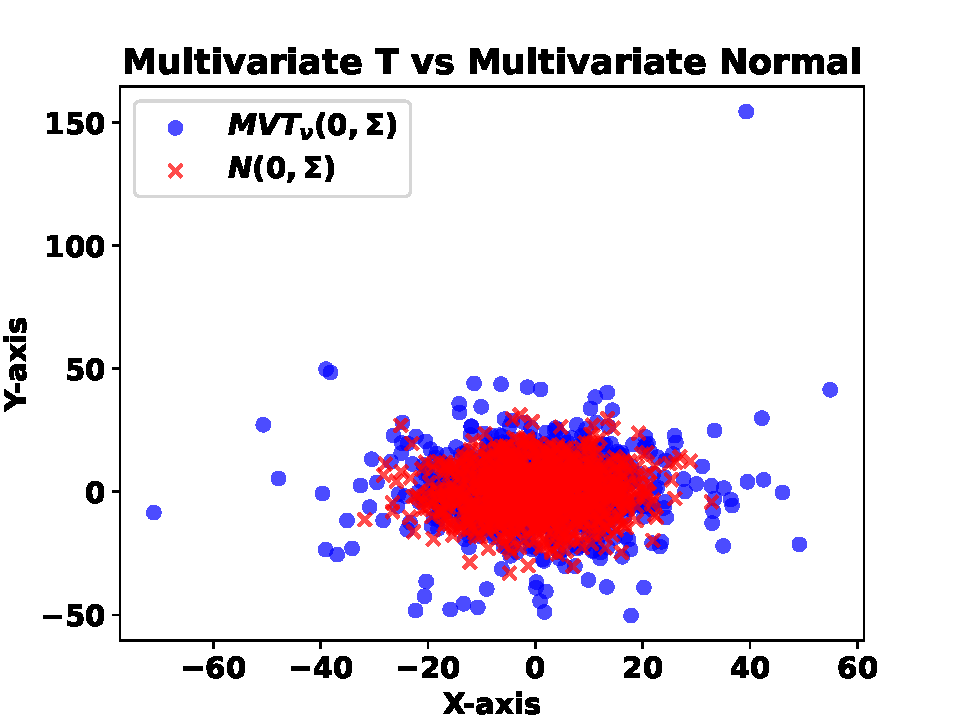
\includegraphics[width=\linewidth]{figuresV2/multivar_t/mvt_vs_normal.pdf}
%     \caption{\textbf{Gaussian vs. Multivariate t Distribution.} Taking $d=2$ and generating $n=1000$ samples from $N(0,\Sigma)$ and $\operatorname{MVT}(\Sigma; \nu=5)$ with $\Sigma$ generated as in Section~\ref{section:gaussian_aux_mle}. The heavier tails of the multivariate t distribution manifests in the outliers relative to the normal distribution.} 
%     \label{fig:enter-label}
% \end{wrapfigure}



\subsubsection{Complexity Analysis}
We analyze the complexity of the discussed CCCP approaches on the example of Algorithm~\ref{alg:aux_multivar_T}. Each outer loop requires computing the term $\gamma \left(\Sigma_k + \hat{\Sigma}_k\right)^{-1} + \frac{n}{2}\Sigma_k^{-1}$ once. This requires two matrix inversions and one matrix addition. Each inner loop requires computing $\nabla f(\Sigma_\ell) + \nabla g(\Sigma_k)$, which can be computed as follows. First, construct a matrix $X = \left( x_1, \ldots, x_n \right) \in \real^{d \times n}$. Second, compute $\Sigma_\ell^{-1}.$ Third, compute the vector $(\nu + x_i^\top \Sigma^{-1}x_i : i \in [n])$ by first computing the quantity 
\[
X \odot \left( \Sigma_\ell^{-1} X \right)
\]
and summing along its last dimension. Call the resulting vector $y$. This requires one matrix multiplication between $d \times d$ and $d \times n$ matrices, one Hadamard product, and $n^2$ scalar additions. For simplicity we can construct the diagonal matrix $D_\ell$ from the following vector
\[
D_\ell \defas \diag\left(\nu + x_i^\top \Sigma^{-1}x_i : i \in [n]\right) = \diag \left(\left(\nu \mathbf{1} + y\right)^{\odot -1} \right) \; ,
\]
where $\odot -1$ denotes element-wise inversion. Finally we obtain 
\[
\sum_{i=1}^n \frac{x_i x_i^\top}{\nu + x_i^\top \Sigma_\ell^{-1} x_i}  = X D_\ell X^\top \; ,
\]
which requires one matrix multiplication between two $n \times d$ matrices.
Then the gradient step requires two additional $d \times d$ matrix products and three matrix-matrix additions. Hence, each inner loop requires at most one matrix inversion and four matrix-matrix multiplications. 


\subsubsection{Log Elliptically Contoured Distributions.}
A \textit{log elliptically contoured distributions} is a probability distribution whose logarithm lies in the class of elliptically contoured distributions. It turns out some log elliptically contoured distributions also satisfy the g-convex and DC structure. One example is the mean zero multivariate log-normal distribution $\text{LogMVN}(0, \Sigma).$ Given i.i.d observations $x_1, \ldots, x_n \in \real^d_{++}$ from $\text{LogMVN}(0, \Sigma)$ its negative log-likelihood $\psi(\Sigma)$ is proportional to 
\begin{equation}\label{eq:log_norm_density}
\psi(\Sigma) \propto \frac{n}{2}\log \det \Sigma + \frac{1}{2}\sum_{j=1}^m \log (x_i)^\top \Sigma^{-1} \log (x_i)
\end{equation}
where we define the operation $\log x_i \in \real^d$ to denote elementwise logarithm.

Observe that the g-convex and DC structure of \eqref{eq:log_norm_density} follows from the fact that $f(\Sigma) = \log \det \Sigma$ is Euclidean concave and g-linear and that the matrix fractional function $g_i(\Sigma) = \log (x_i)^\top \Sigma^{-1} \log (x_i)$ is Euclidean convex for each $1 \leq i \leq d.$ The g-convexity of $g_i(\Sigma)$ follows from it being a g-convex atom (see Example~\ref{example:g_cvx_atoms}(6)).

Hence one can also derive an algorithm like Algorithm~\ref{alg:CCCP_on_MLE} and Algorithm~\ref{alg:CCCP_on_Kotz} to solve the \emph{log-normal optimistic likelihood} optimization problem 
\[
\begin{aligned}
    &\argmin_{\Sigma \in \pd} \Psi(\Sigma) + \beta \delta_S^2(\Sigma, \hat{\Sigma})
    \\& \text{where} \quad \Psi(\Sigma) \defas \frac{n}{2}\log\det \Sigma + \frac{1}{2}\sum_{j=1}^m \log(x_i)^\top  \Sigma^{-1} \log (x_i)
\end{aligned}
\]
where $\beta >0$ is our regularization hyperparameter.

\subsection{Linear Regression on the $\pd$ manifold.}\label{section:linear_regression}
Our framework naturally encompasses linear regression on the manifold of positive definite matrices endowed with the affine invariant metric \cite{regression_pd}. 
Let $X \in \real^{d \times d}$ be our data and $y \in \real$ be our observed target. We aim to minimize the quadratic loss function $f(\hat{y}, y) = \frac{1}{2}\left(\hat{y}-y\right)^2$. For simplicity, we consider the model 
\begin{equation}
\hat{y} = f(W) = \tr(WX) \; , 
\end{equation}
wherein the least square problem becomes: 
\begin{equation}\label{eq:regression_pd}
\min_{W \in \pd} \frac{1}{2}\left(\tr(W \operatorname{Sym}(X)) - y\right)^2   
\end{equation}
with $\operatorname{Sym}(X) = \frac{X + X^\top}{2}$ (see~\cite[sec. 5]{regression_pd} for more details). The flexibility of our structured regularization framework allows us to regularize \eqref{eq:regression_pd} to incorporate side information. For instance, if we are given an estimator $\hat{W} \in \pd$ we can reformulate the problem as
%
\begin{equation}\label{eq:regression_aux}
    \min_{W \in \pd} \frac{1}{2}\left(\tr\left(W \operatorname{Sym}(X)\right) - y\right)^2 + \beta d_{\Phi}(W, \hat{W}) 
\end{equation}
for a specified symmetric gauge function $\Phi$ (see Section~\ref{sec:SG_Ball_Constraints}). Based on our discussions about its computational advantages and similarity to the Riemannian distance (see Section~\ref{sec:ball_constraint_sdiv}), one can replace $d_\Phi$ with the S-divergence, $\delta_S^2$, i.e., a regularizer based on symmetric gauge functions (see Example~\ref{ex:sdiv}).

Moreover, we can induce sparsity by adding a sparsity inducing regularizer $R_\Phi(W)$, obtaining
\begin{equation}\label{eq:regression_sparse}
    \min_{W \in \pd} \frac{1}{2}\left(\tr\left(W \operatorname{Sym}(X)\right) - y\right)^2 + \beta R_{\Phi}(W) \; .
\end{equation}
We note that since $d_\Phi$ and $R_\Phi$ are g-convex regularizers, the resulting optimization problems  \eqref{eq:regression_aux}  and \eqref{eq:regression_sparse} are both g-convex and hence can be solved using standard first-order Riemannian iterative methods. However, if one specifies $d_\Phi$ in \eqref{eq:regression_aux} to be the S-divergence regularizer
or replace $R_\Phi(W)$ with the diagonal loading regularizer (see Example~\ref{prop:diagonal_loading}) then the objective becomes g-convex \textit{and} DC.


One can adapt \eqref{eq:regression_aux} or \eqref{eq:regression_sparse} to the kernel learning or Mahalanobis distance learning problem (see sections 9.1 and 9.2 \cite{regression_pd}). For example, one can use \eqref{eq:regression_aux} to \emph{anchor} the solution to $\hat{W} \in \pd$ where $\hat{W}$ is an estimated Mahalanobis matrix from an auxiliary dataset that is representative of the data of interest. Alternatively, one can use \eqref{eq:regression_sparse} to encourage convergence to low-rank Mahalanbois matrices.


%\mw{It would be great to add 1-2 sentences on applications where the respective type of "extra information" arises.}




\section{Experiments}

\subsection{Square Root Problem}
We consider the problem of computing the square root of a matrix $A \in \pd$. 
 In this section, we demonstrate the competitive performance of CCCP against standard first-order Riemannian approaches for this problem. Recall that in this case, the CCCP oracle can be solved in closed form, rendering CCCP into a simple fixed point approach (see Eq.~\ref{eq:sqrt_fp}).


\paragraph{Data Generation}
We generate both medium-conditioned and ill-conditioned data. In the \textit{medium-conditioned} case, we construct 
\[
A = G G^\top \qquad \text{where} \qquad G_{ij} \stackrel{\text{i.i.d.}}{\sim} N(0,1).
\]
We further consider the Hilbert matrix
\[
H_{ij} = \frac{1}{i+j-1} \; ,
\]
a notable example of a very ill-conditioned matrix.
 

 \paragraph{Results}
 We showcase the performance of computing the square roots $A^{\frac{1}{2}}$ and $H^{\frac{1}{2}}$ with CCCP and benchmark against two Riemannian Conjugate Gradient (RCG) and Riemannian Gradient Descent (RGD).

Figures~\ref{fig: square_root_exp_medium} and \ref{fig: square_root_exp_ill} give results for all three algorithms in both cases. The stepsizes for RGD and RCG are determined by backtracking line search. In contrast, the fixed-point algorithm does not require a stepsize. As a reference point, the true optimum $X^*$ is computed using NumPy's square root function. The CCCP algorithm exhibits superior performance in terms of runtime. In the ill-conditioned case, we observe that RGD and RCG are unable to converge to the optimum. In contrast, CCCP attains the optimum even for ill-conditioned data. We believe this is due to the fact that the fixed-point algorithm computes the inverse of $X_k + A$ (medium-conditioned) rather than of $A$ (ill-conditioned), which is required by the gradient-based methods. This is illustrated in Figure~\ref{fig:cond_num_sqrt} and particularly evident, if we cross-compare the accuracy achieved by the three approaches:
\[
\begin{aligned}
    &\|H - \hat{H}_{\operatorname{CCCP}}\|_{F} = 8.9 \times 10^{-5}
    \\&\|H - \hat{H}_{\operatorname{RGD}}\|_{F} = 129.791
    \\&\|H - \hat{H}_{\operatorname{RCG}}\|_{F} = 126.335 
\end{aligned} \; .
\]
We discuss this observation in more detail in the next section.

% \begin{figure}[ht]
%     \centering
%     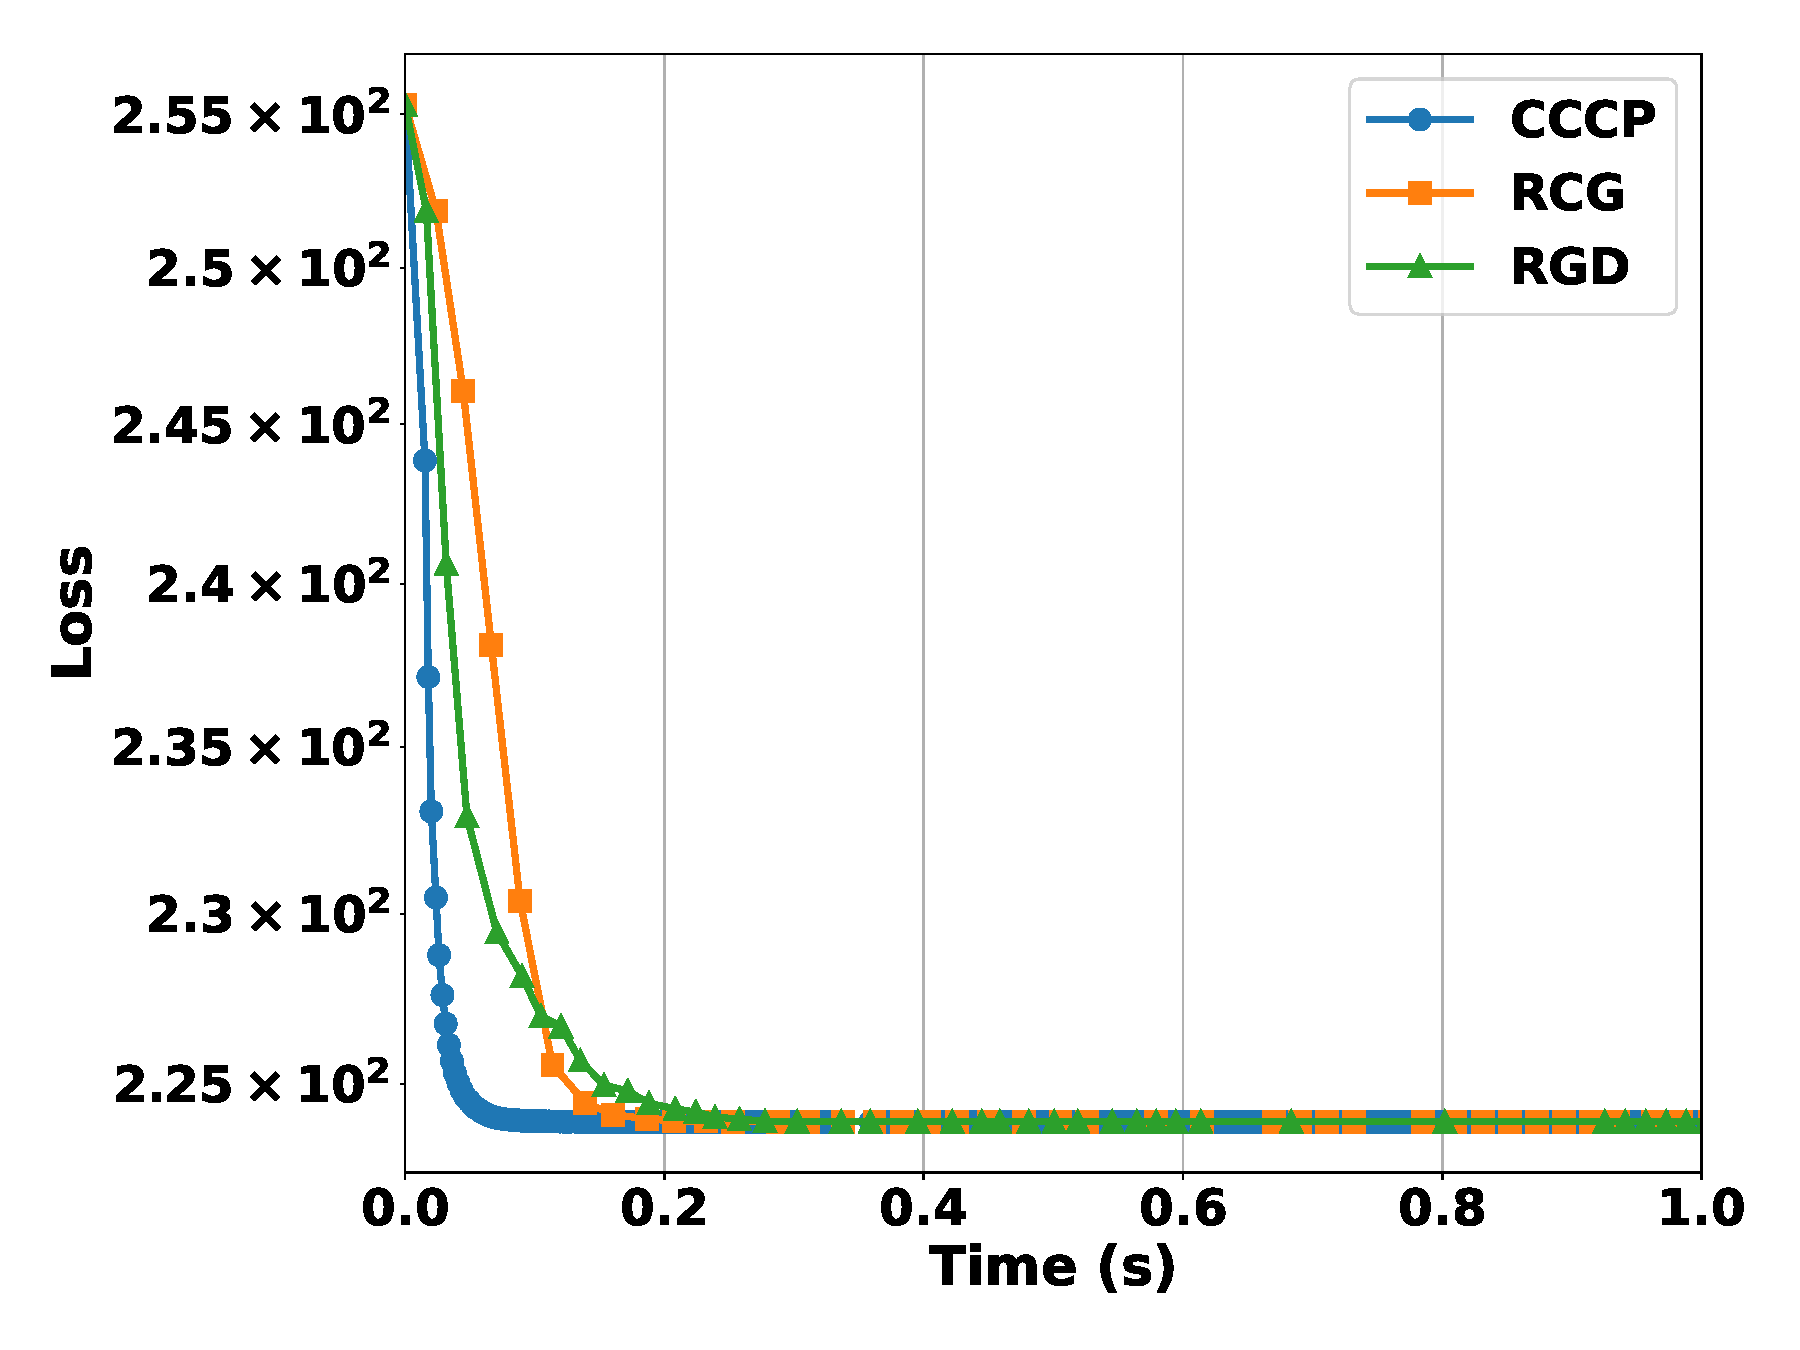
\includegraphics[height=5cm]{figuresV2/square_root/loss_time_200_medium.pdf} 
%     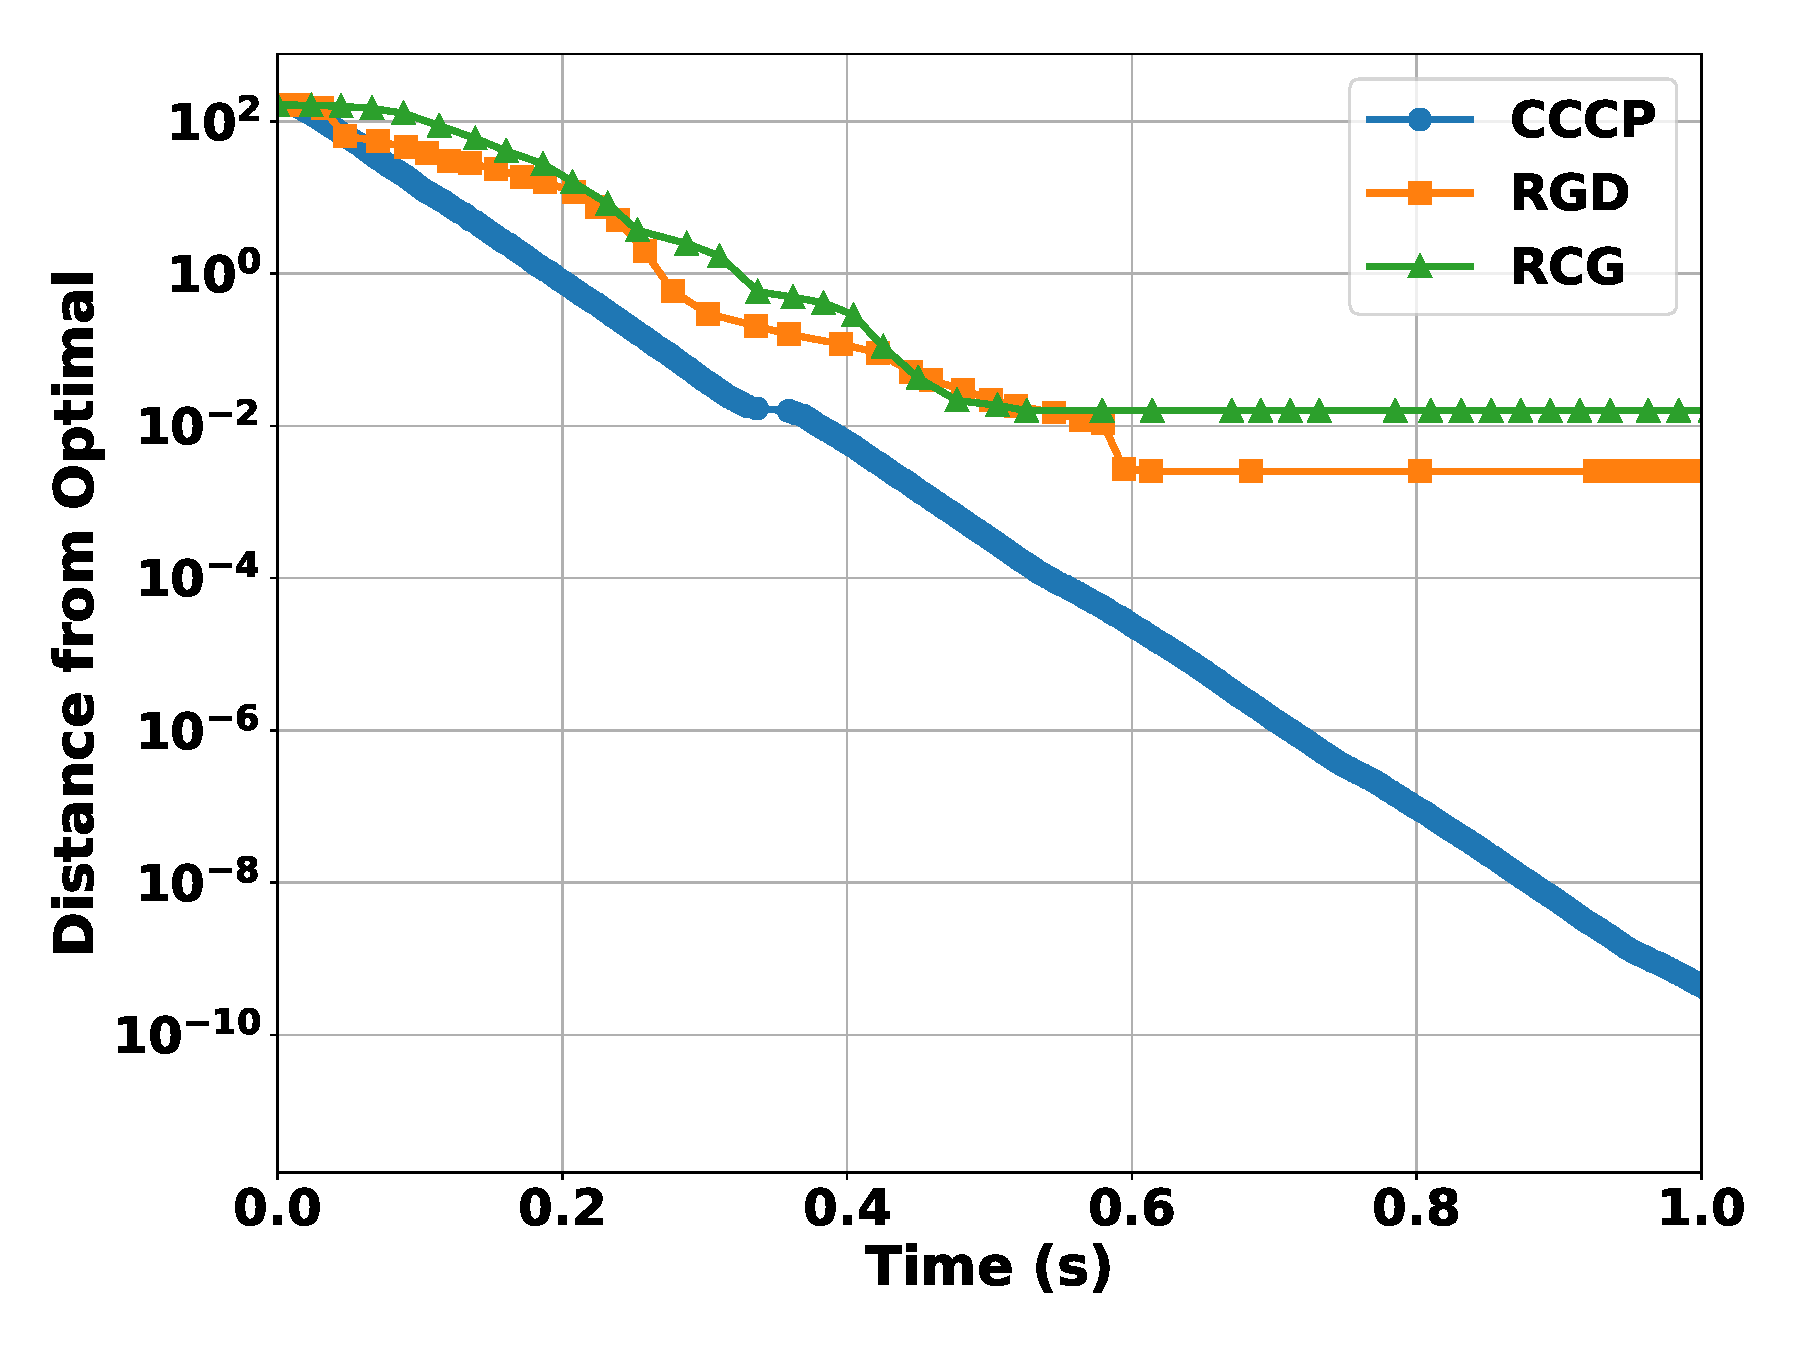
\includegraphics[height=5cm]{figuresV2/square_root/distance_time_200_medium.pdf}\\
%      \caption{We apply the fixed-point algorithm (see Proposition~\ref{prop:fp_sqrt}) to the medium conditioned $H \in \real^{200 \times 200}$. We initialized all algorithms at $X_0 = 3 I_d$. We observe that all three methods perform comparatively in terms of iteration-complexity. The fixed-point method is superior in terms of runtime.}
%     \label{fig: square_root_exp_medium}
% \end{figure}



\begin{figure}[htbp]
  \centering
  \begin{minipage}[b]{0.45\textwidth}
    \centering
    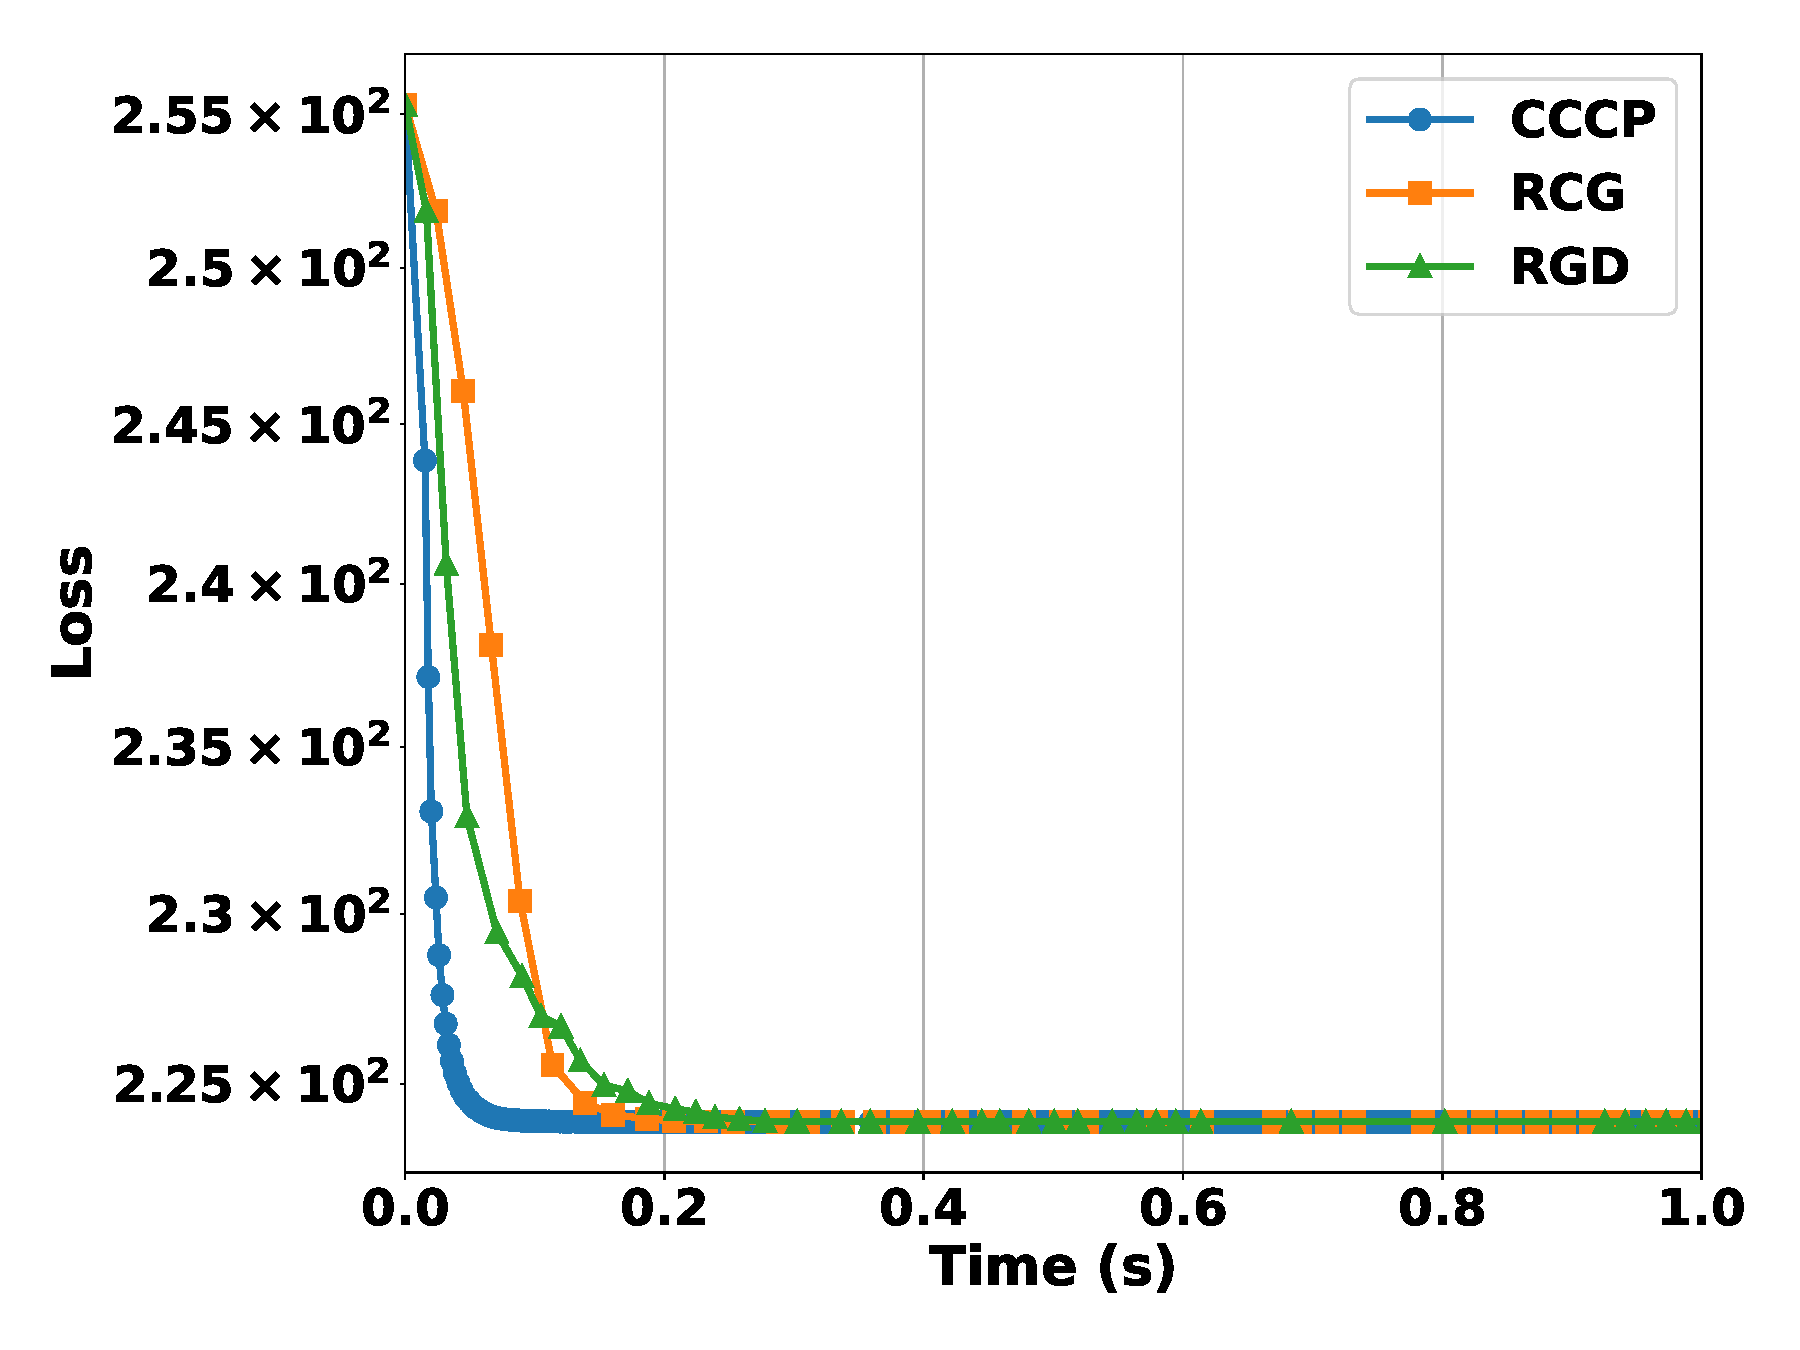
\includegraphics[width=\textwidth]{figuresV2/square_root/loss_time_200_medium.pdf}
  \end{minipage}
  \hfill
  \begin{minipage}[b]{0.45\textwidth}
    \centering
    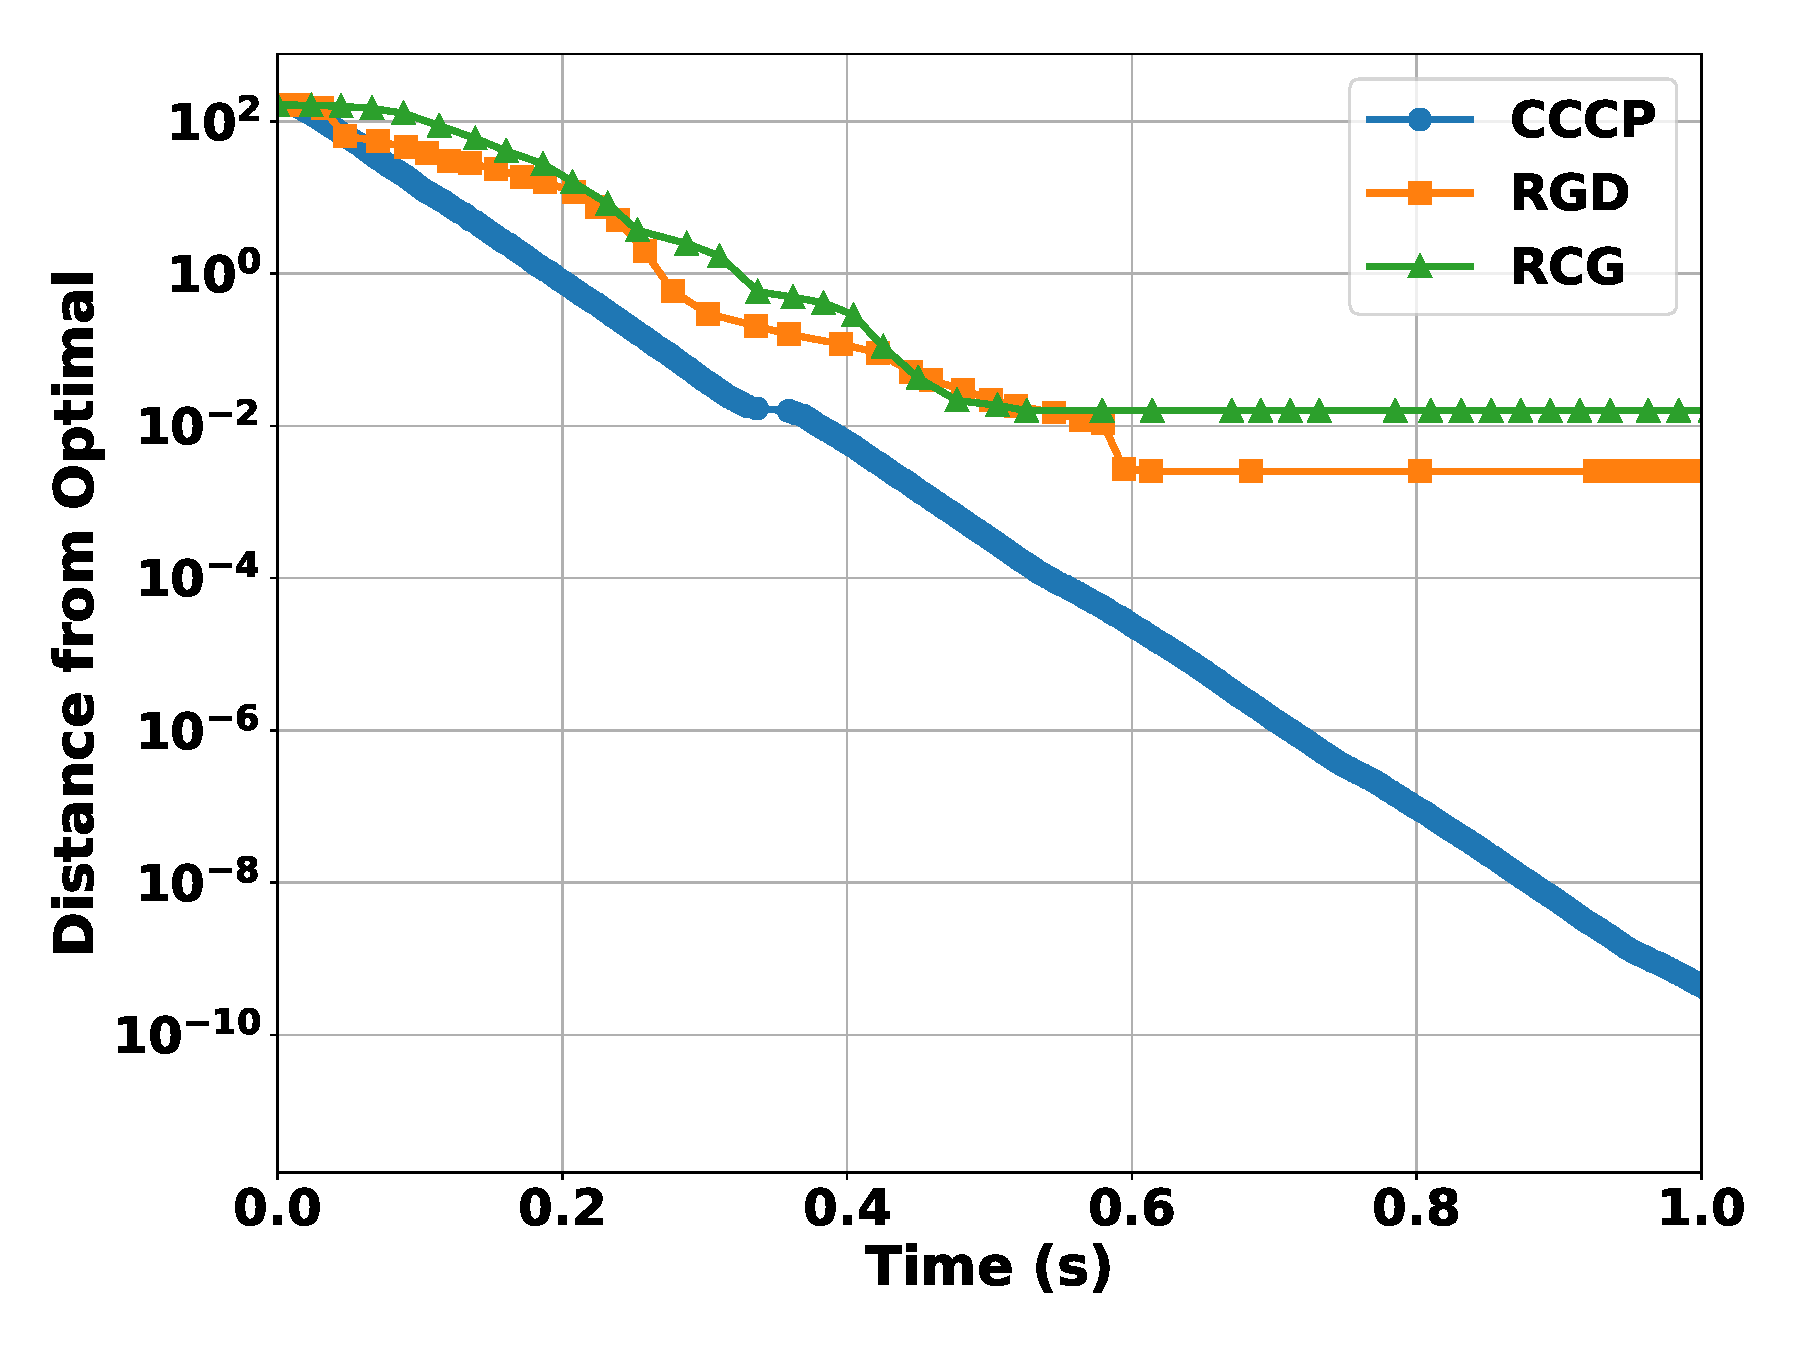
\includegraphics[width=\textwidth]{figuresV2/square_root/distance_time_200_medium.pdf}
  \end{minipage}
  \caption{We apply the fixed-point algorithm (see Proposition~\ref{prop:fp_sqrt}) to the medium conditioned $H \in \real^{200 \times 200}$. We initialized all algorithms at $X_0 = 3 I_d$. Although all three methods are of the same order in terms of per-iteration-complexity, the fixed-point method exhibits superior runtime performance. The stepsizes for RGD and RCG are chosen using backtracking line search. In contrast, the fixed-point algorithm does not need a stepsize. Distance is measured in terms of the Frobenius norm.}
    \label{fig: square_root_exp_medium}
\end{figure}






% \begin{figure}[ht]
%     \centering
%     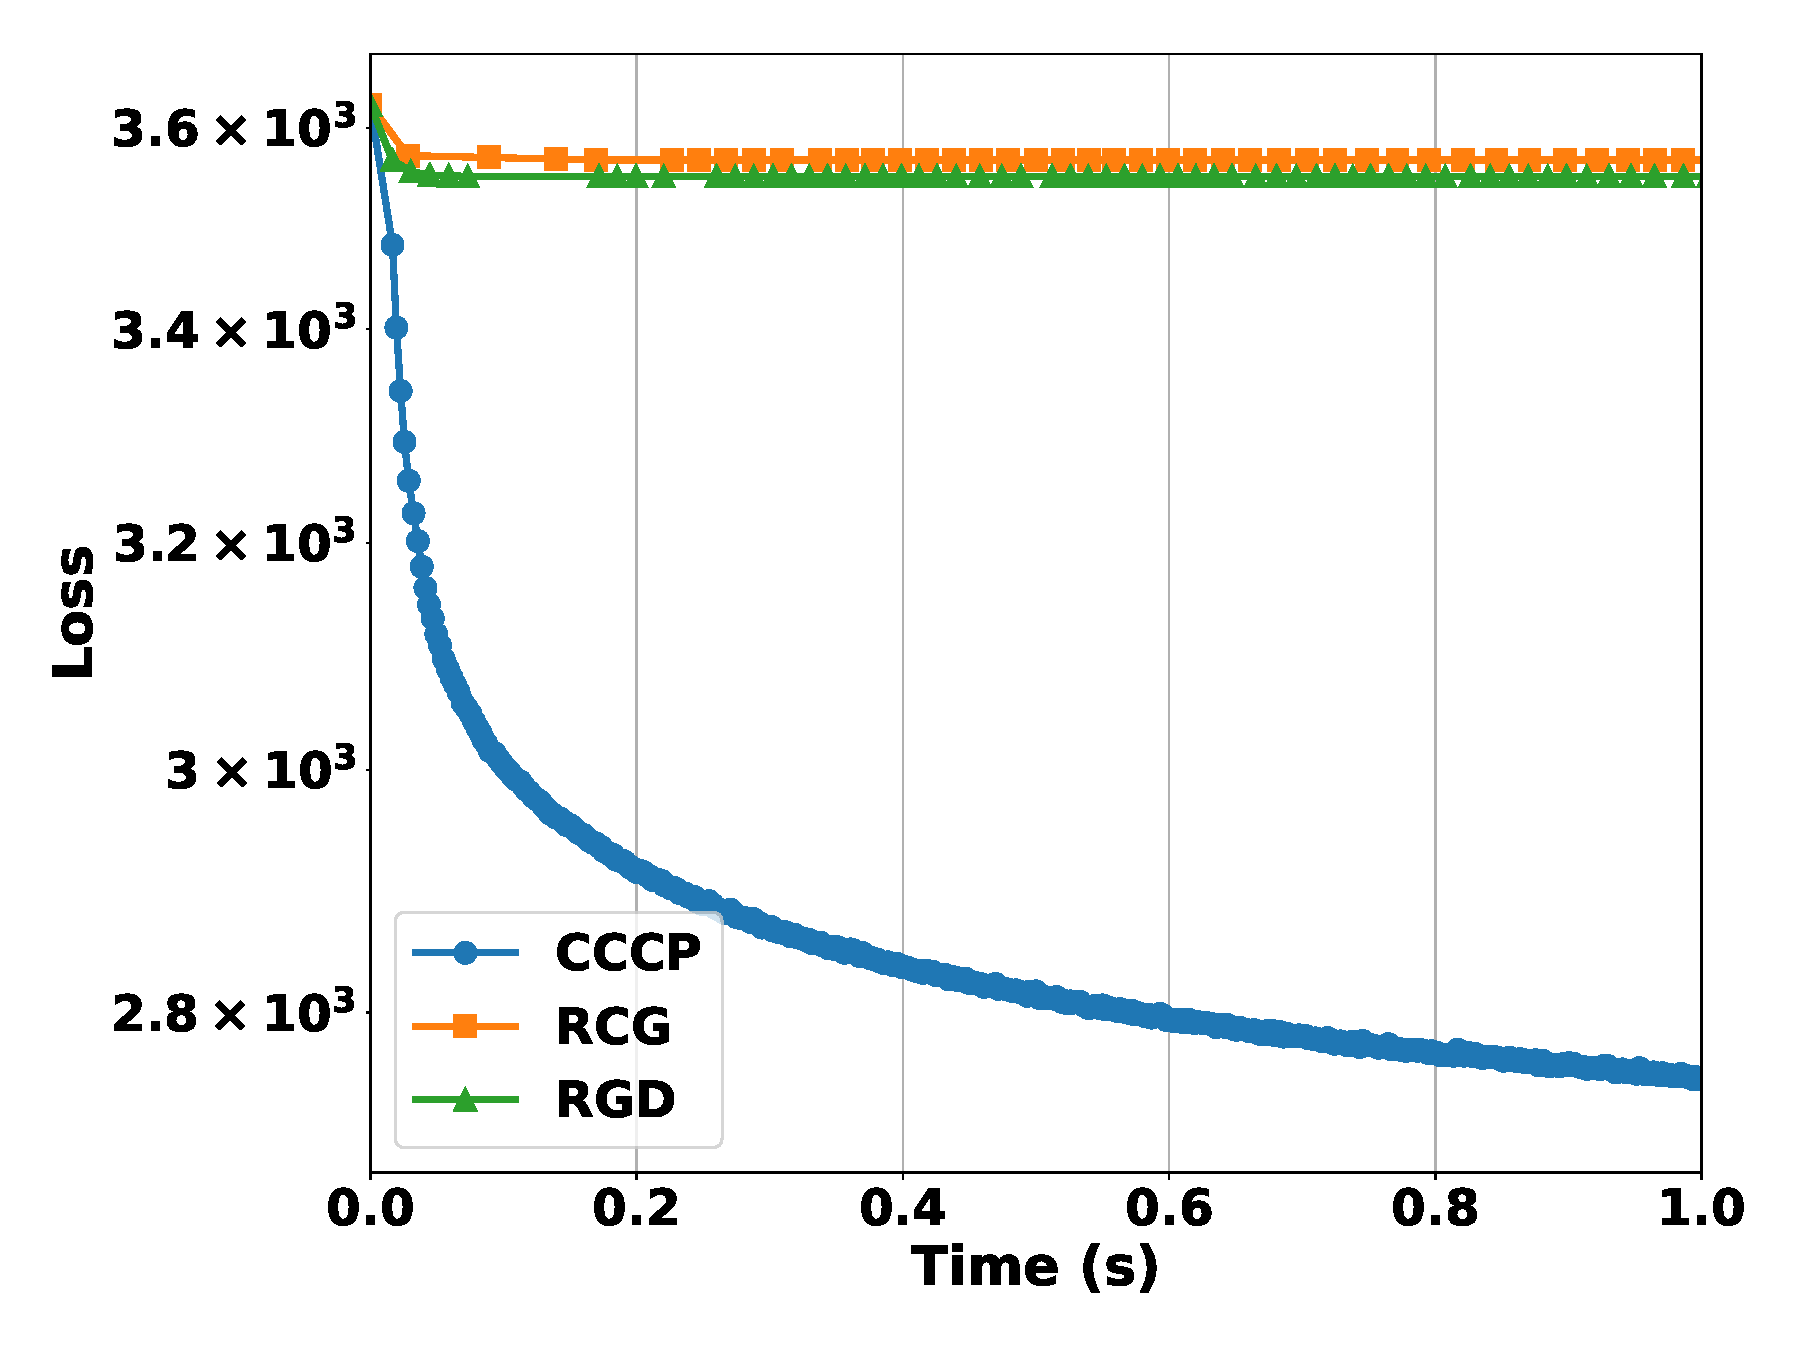
\includegraphics[height=5cm]{figuresV2/square_root/loss_time_200_ill.pdf} 
%     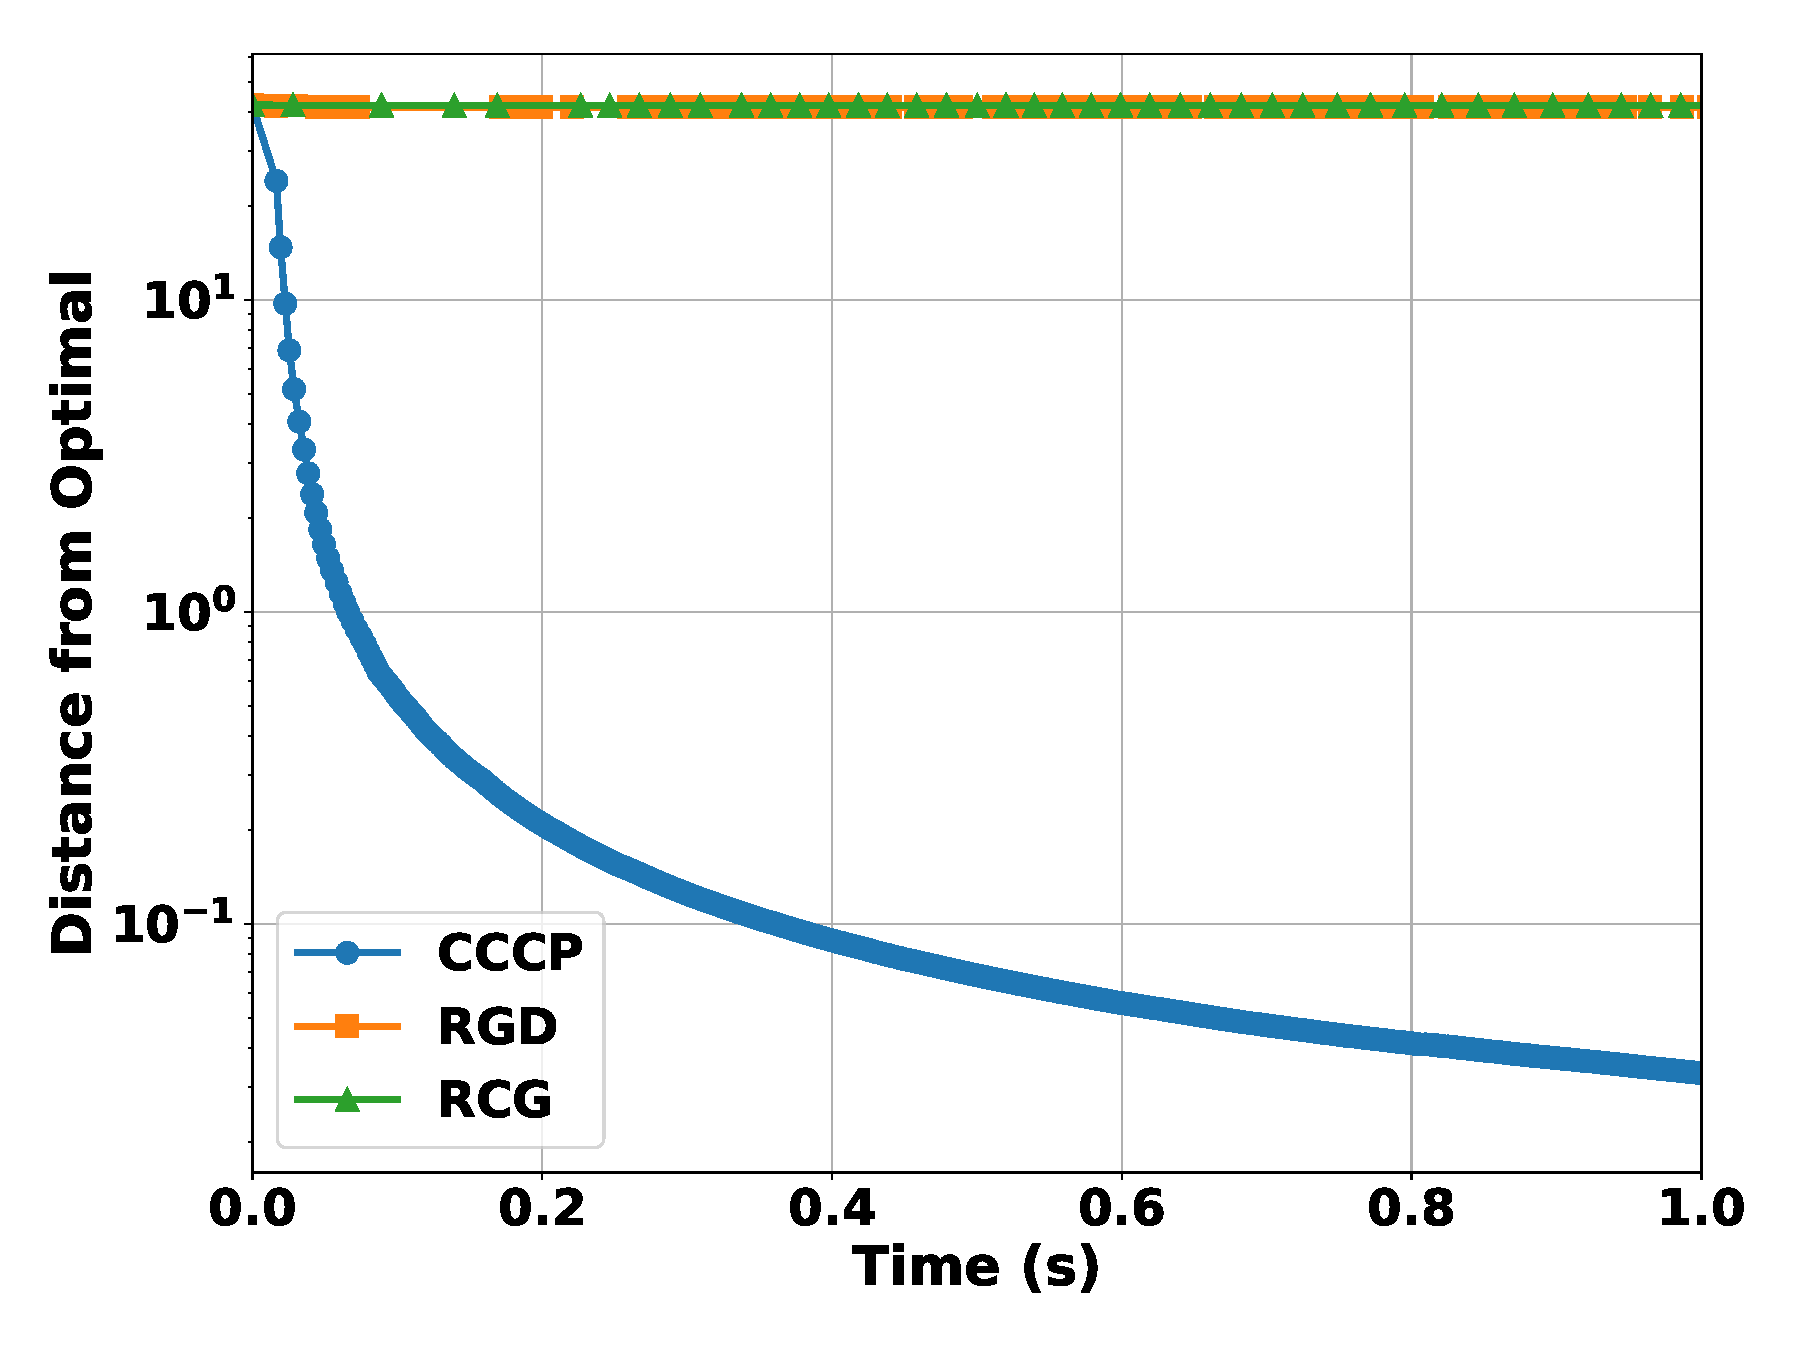
\includegraphics[height=5cm]{figuresV2/square_root/distance_time_200_ill.pdf}\\
%      \caption{We apply the fixed-point algorithm (see Proposition~\ref{prop:fp_sqrt}) to the ill conditioned Hilbert matrix where we took dimension $d=200$. We initialized all algorithms at $X_0 = 3 I_d$. The benchmarks fail to converge whereas. CCCP exhibits robustness to ill conditioning.}
%     \label{fig: square_root_exp}
%     \label{fig:enter-label}
% \end{figure}

\begin{figure}[htbp]
  \centering
  \begin{minipage}[b]{0.45\textwidth}
    \centering
    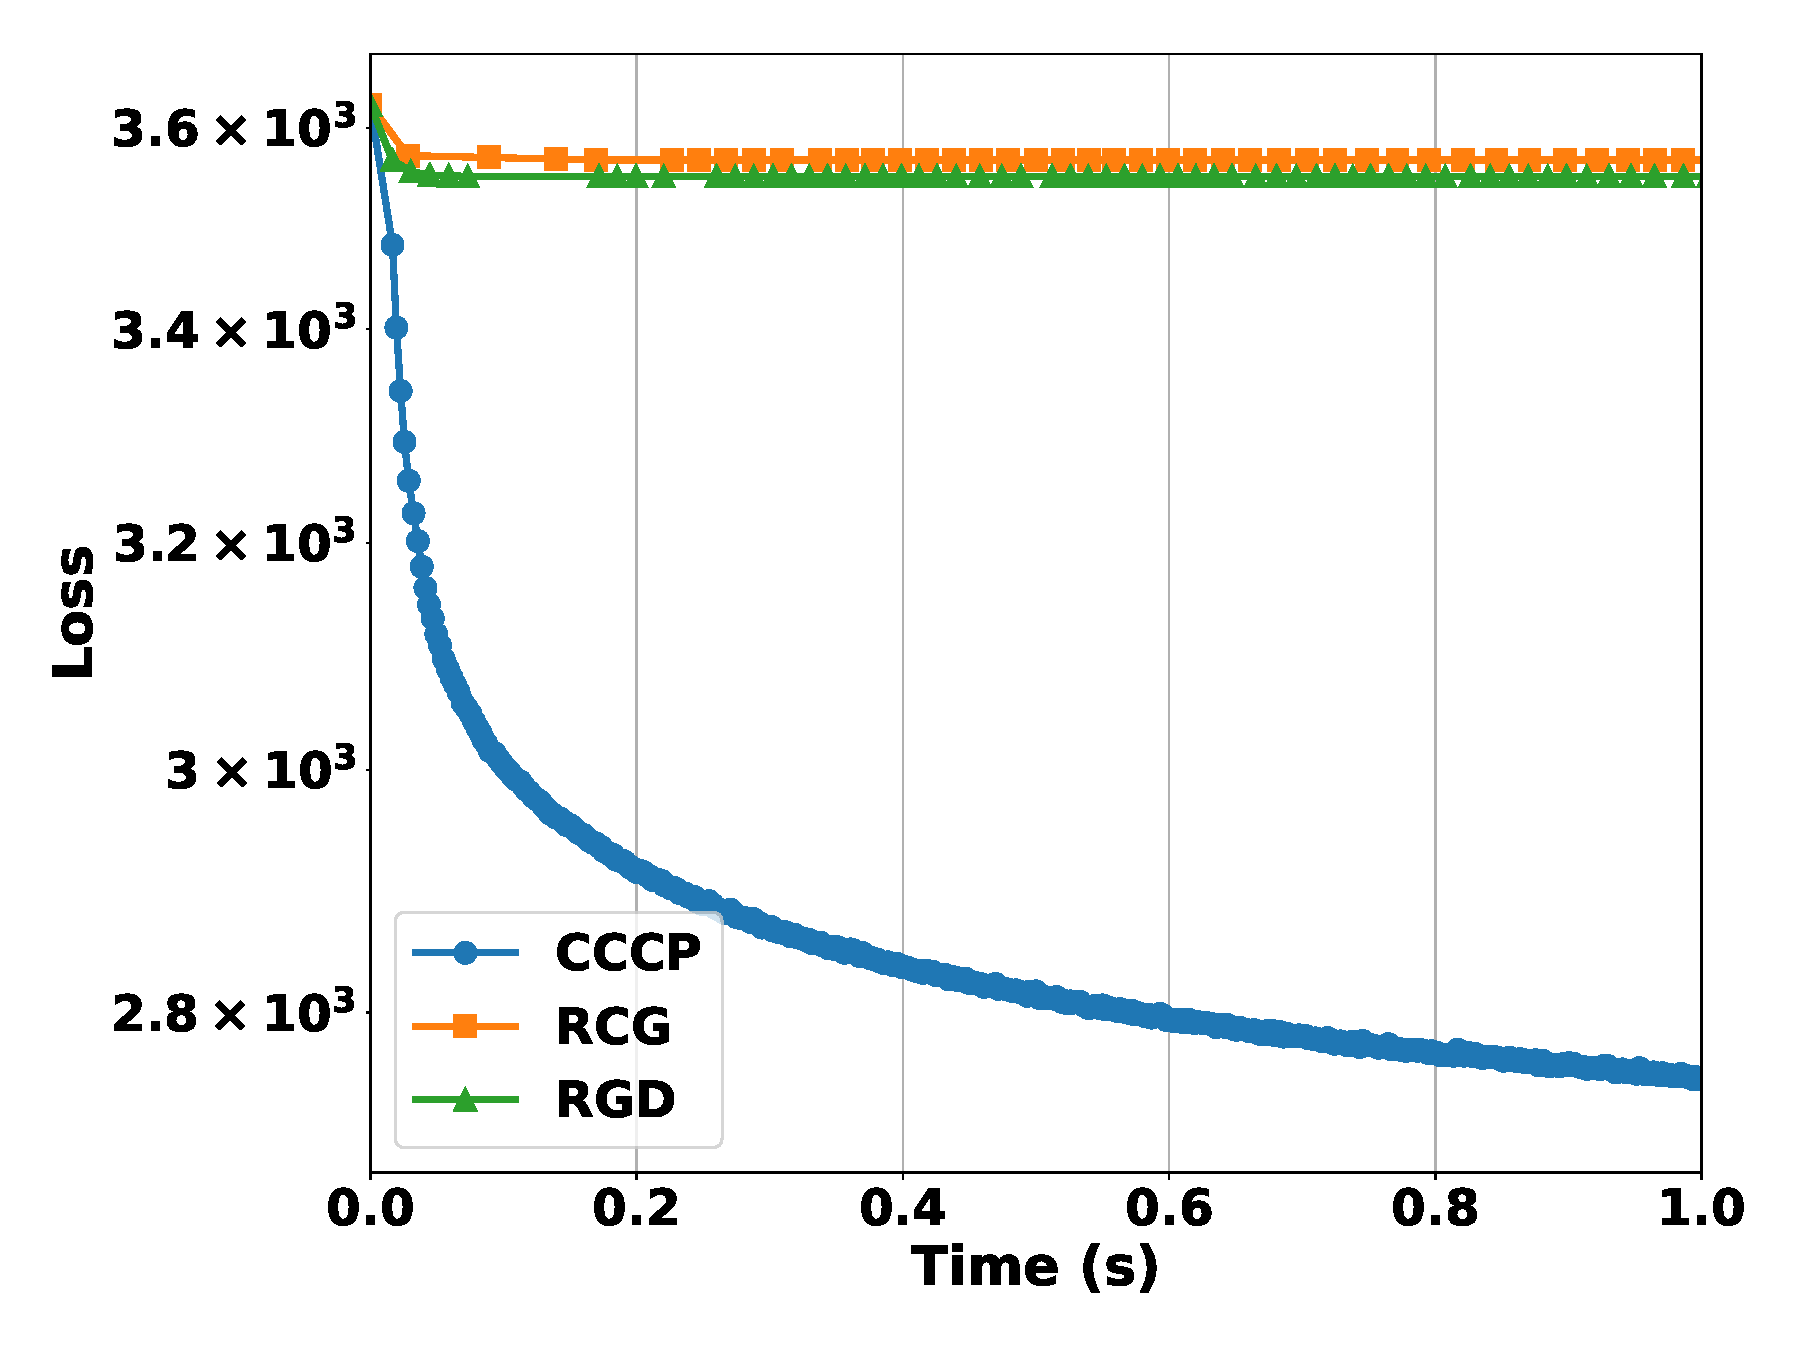
\includegraphics[width=\textwidth]{figuresV2/square_root/loss_time_200_ill.pdf}
  \end{minipage}
  \hfill
  \begin{minipage}[b]{0.45\textwidth}
    \centering
    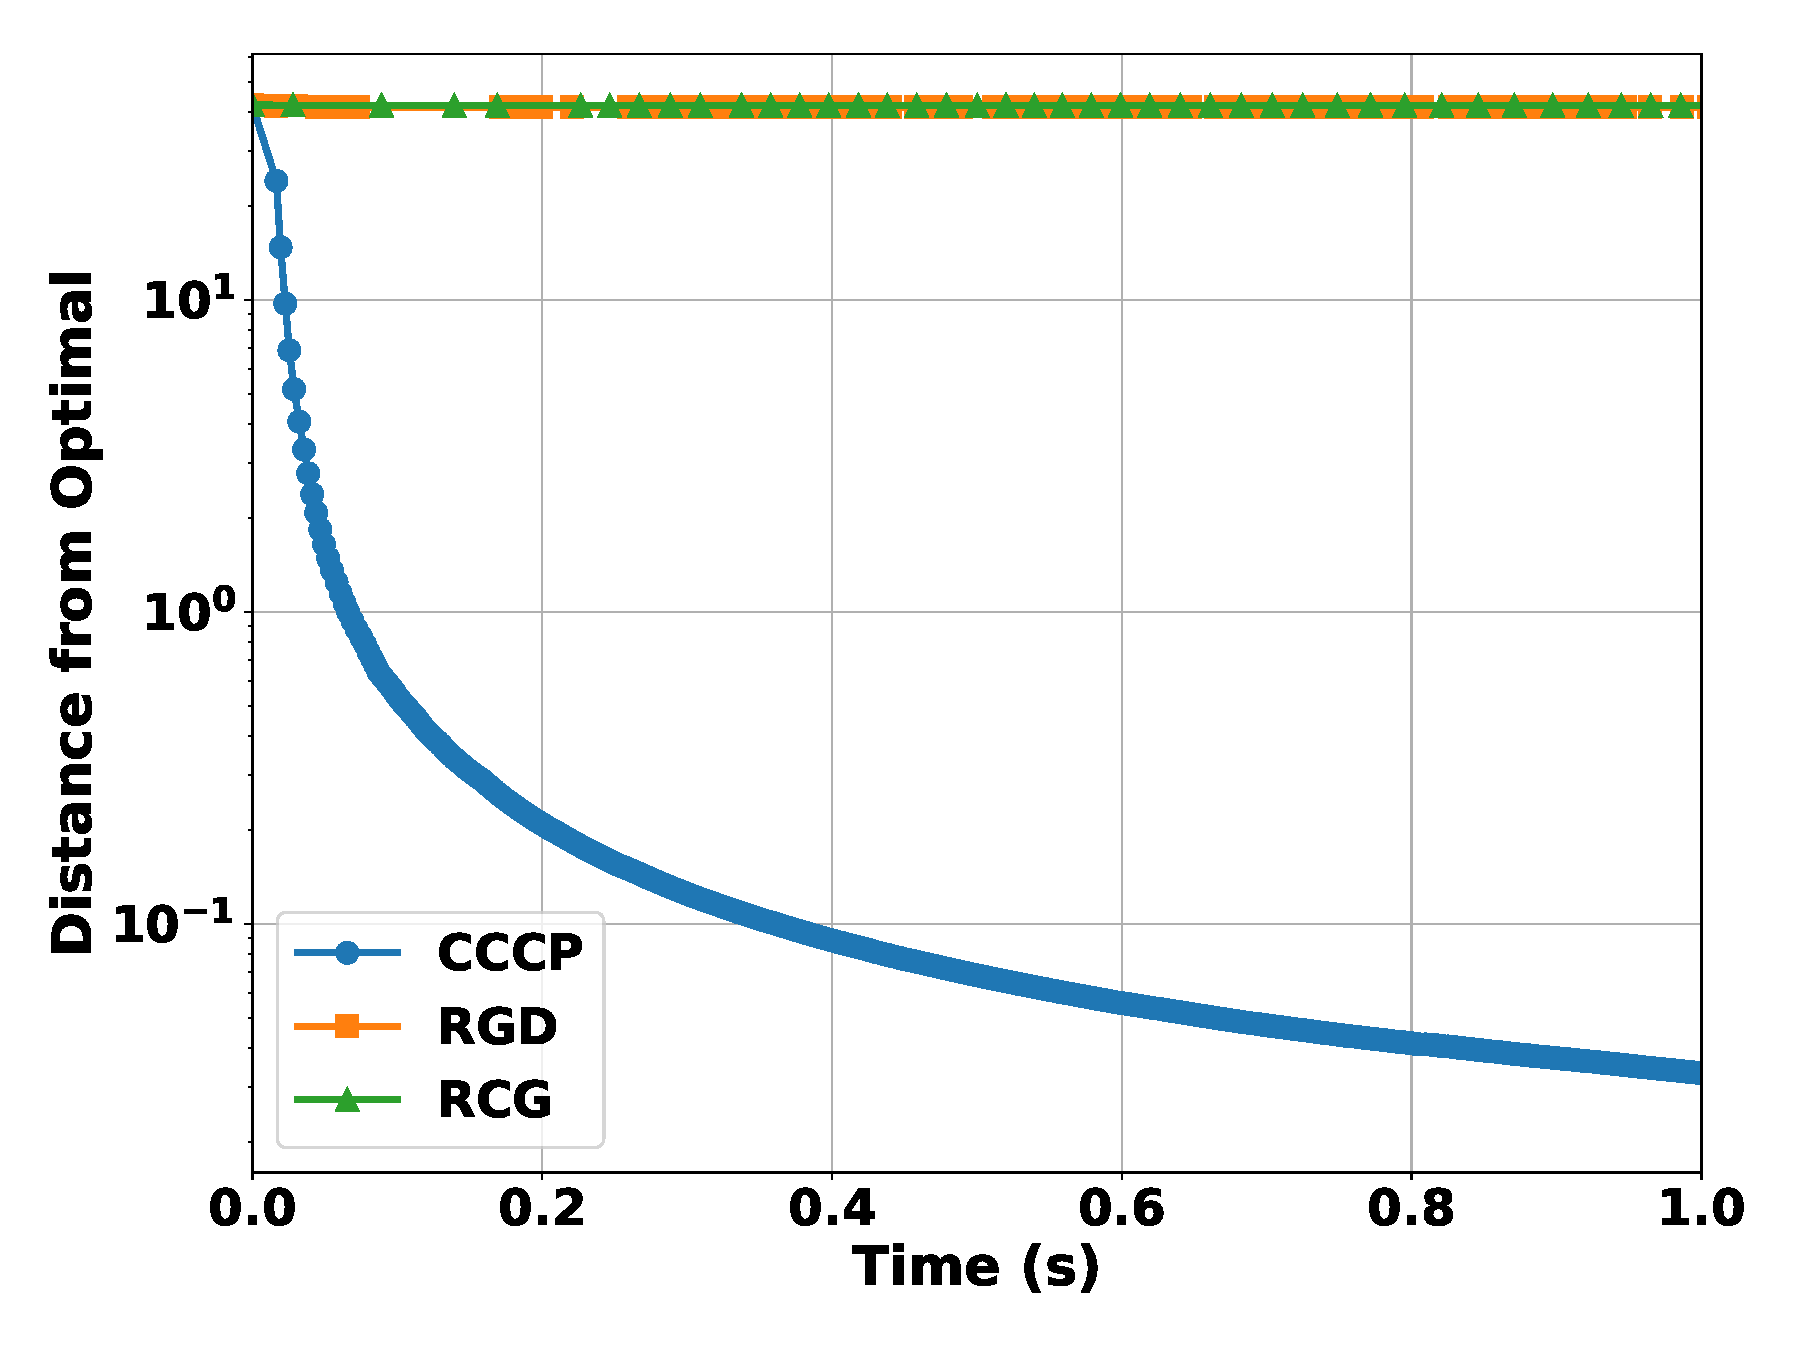
\includegraphics[width=\textwidth]{figuresV2/square_root/distance_time_200_ill.pdf}
  \end{minipage}
  \caption{We apply the fixed-point algorithm (see Proposition~\ref{prop:fp_sqrt}) to the ill-conditioned Hilbert matrix where we took dimension $d=200$. We initialized all algorithms at $X_0 = 3 I_d$. The benchmarks fail to converge whereas CCCP exhibits robustness to ill conditioning.}
  \label{fig: square_root_exp_ill}
\end{figure}





% \begin{figure}[ht]
%     \centering
%     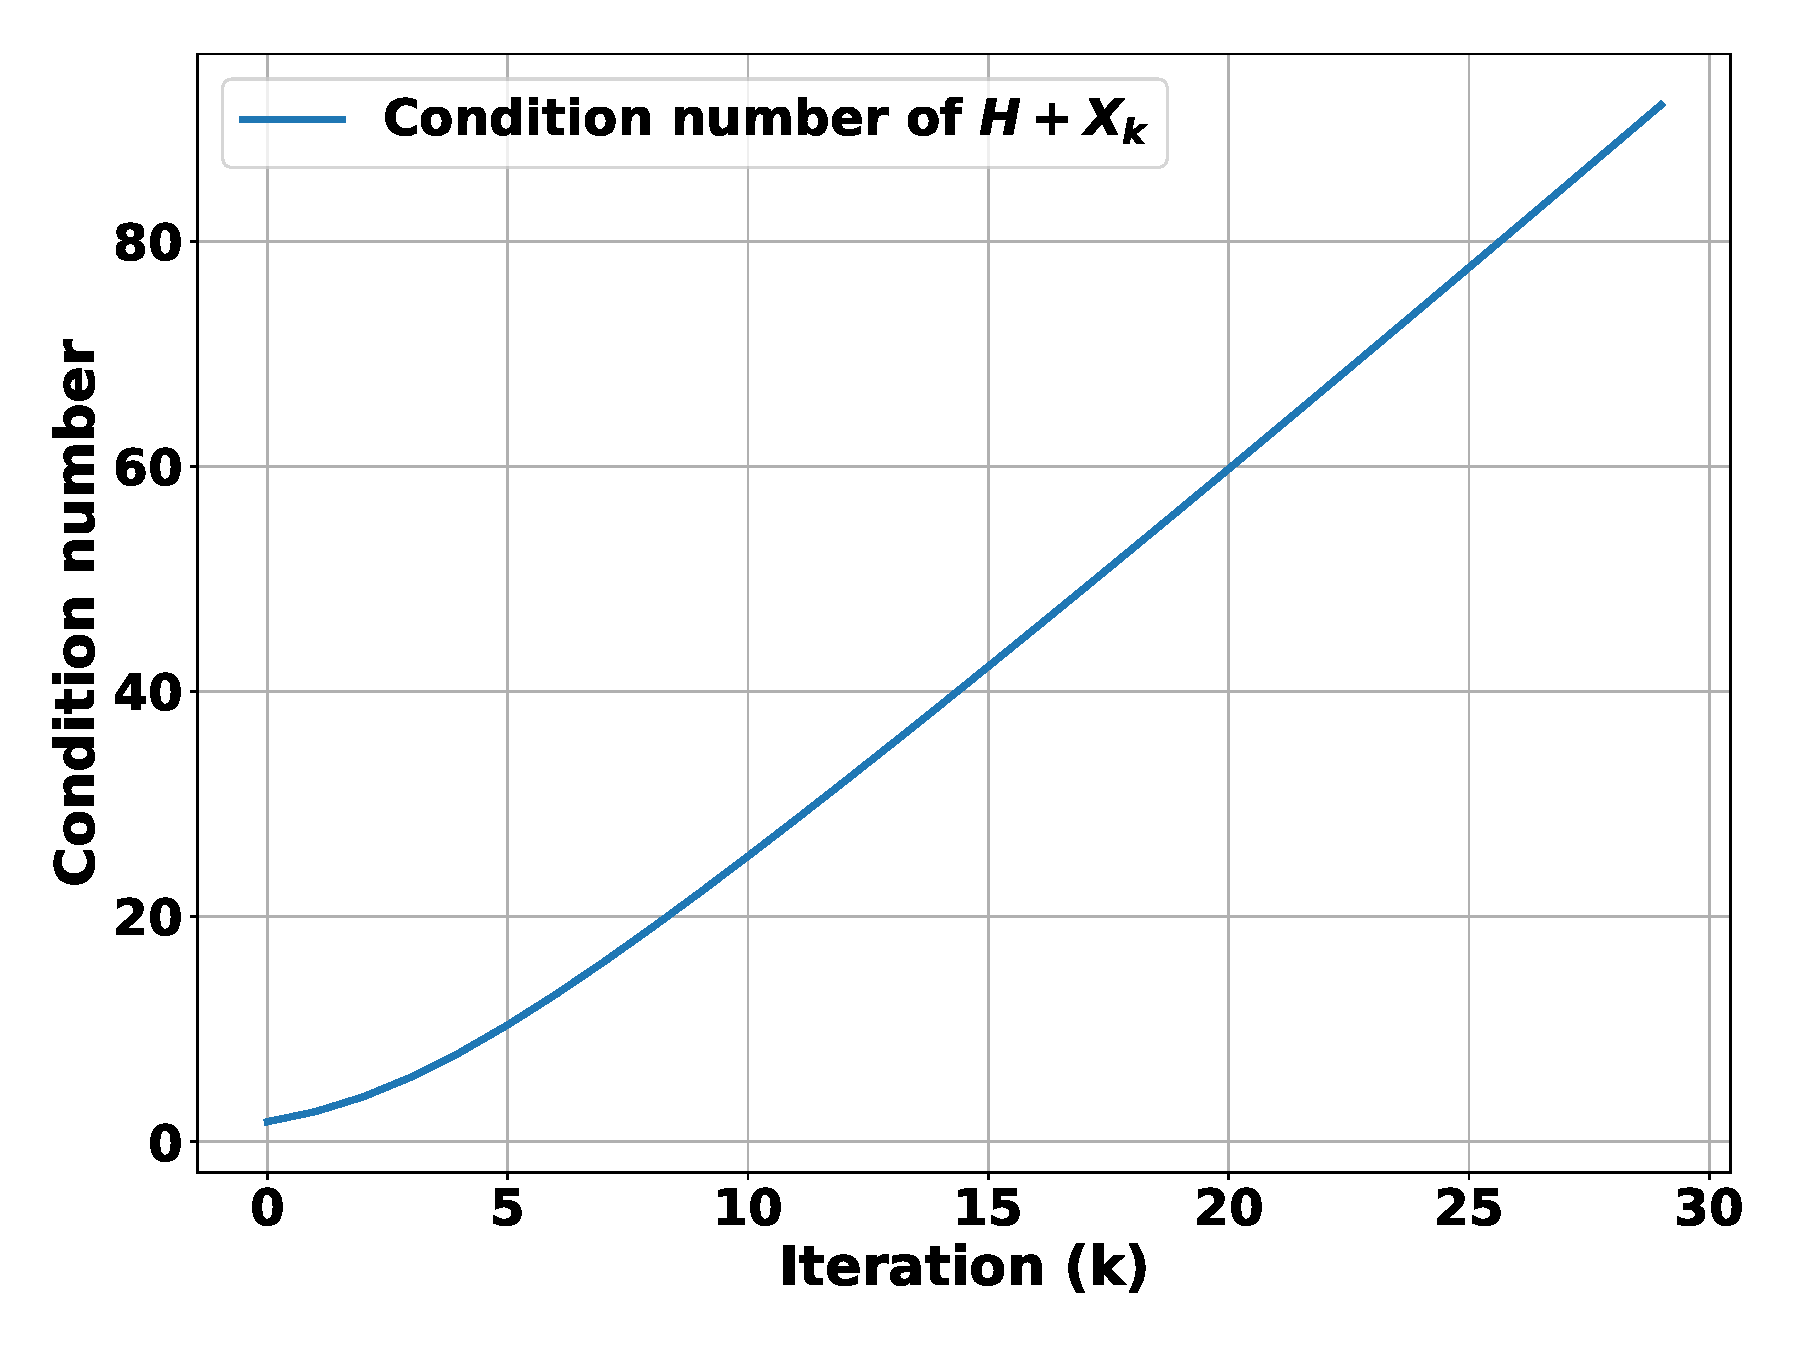
\includegraphics[height=5cm]{figures/A_rankK.pdf}
%     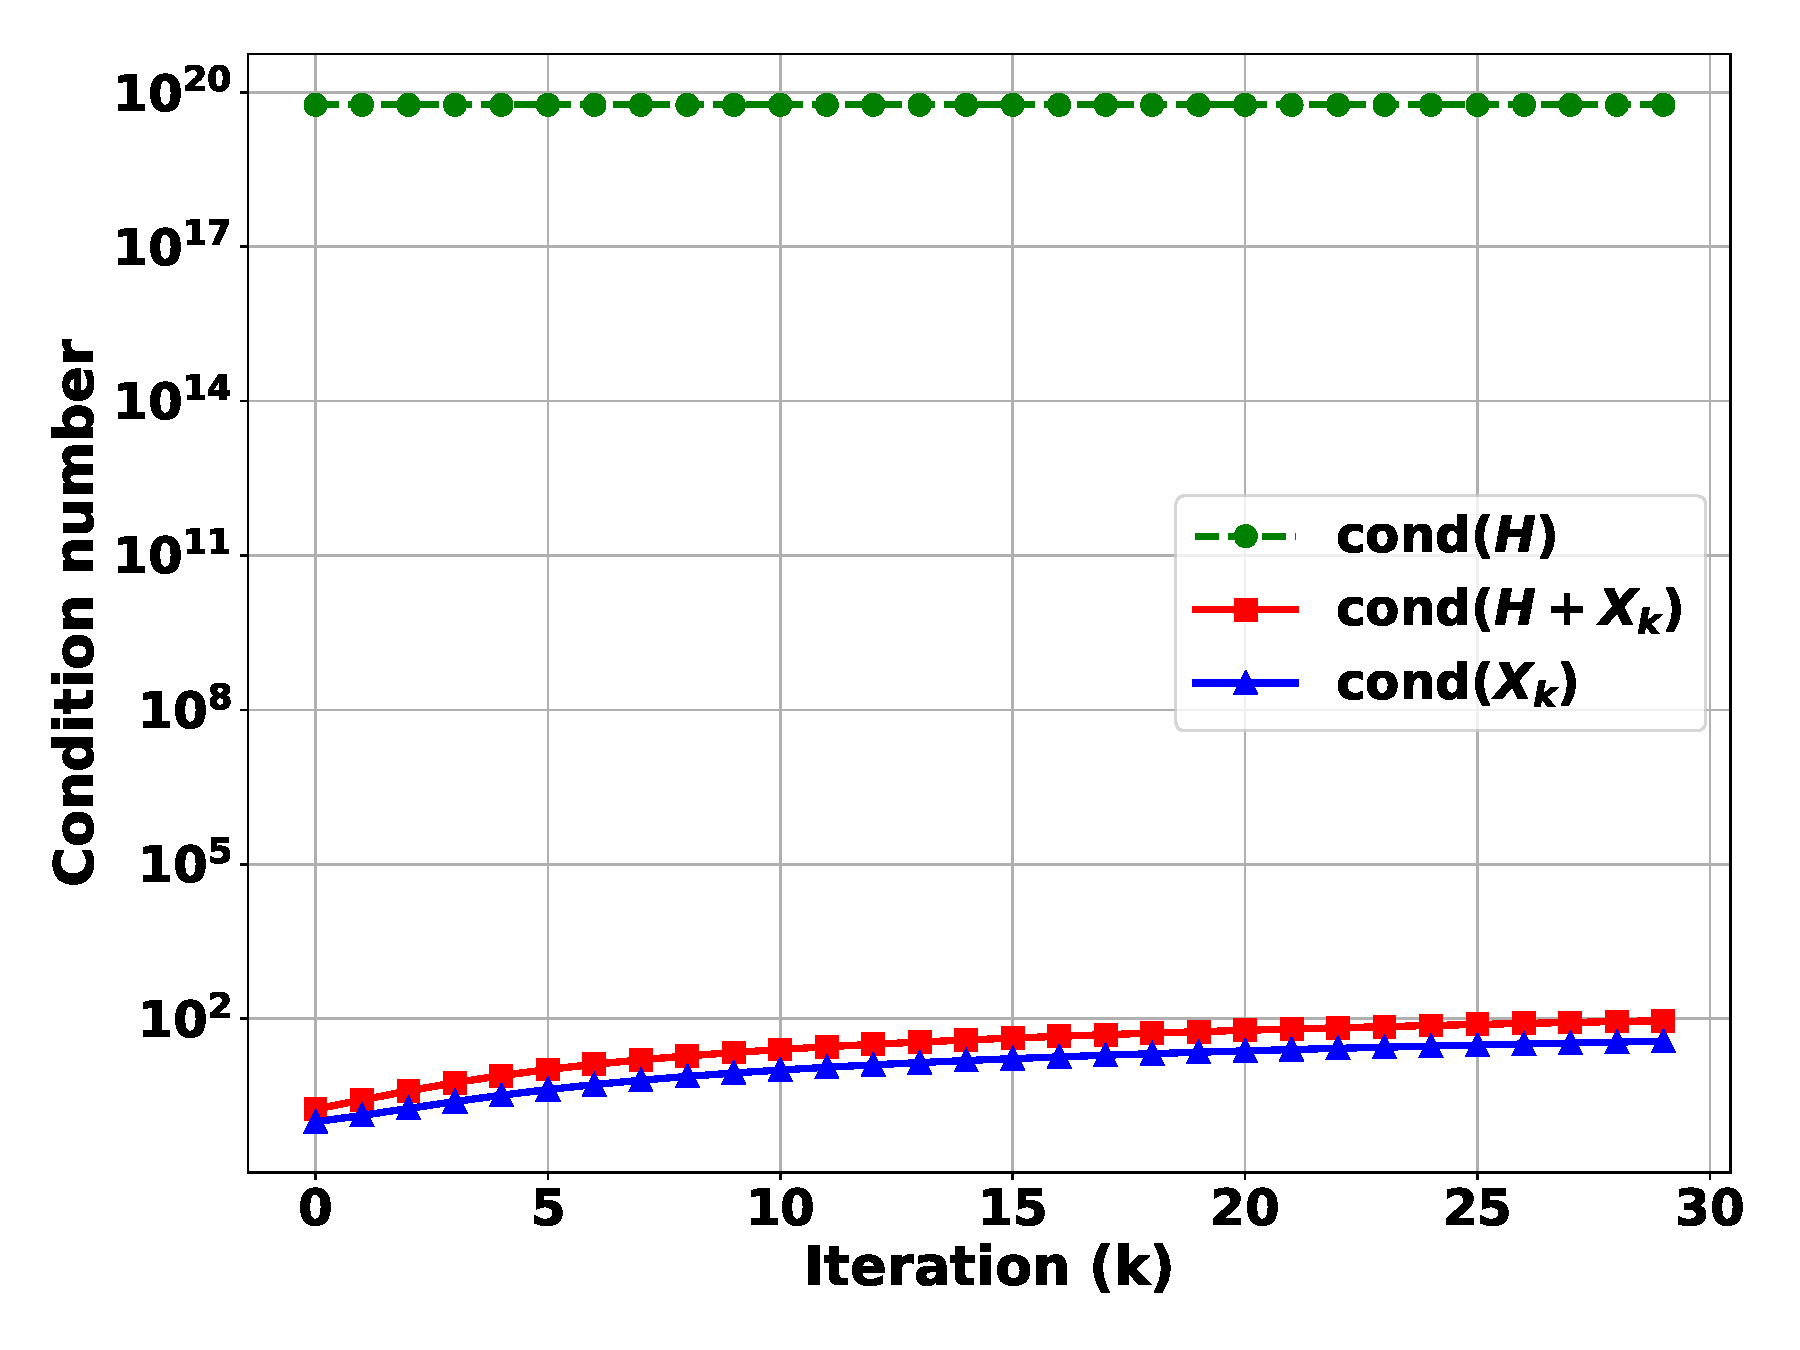
\includegraphics[height=5cm]{figures/A_X_rankK.pdf}
%     \caption{We use the ill-conditioned Hilbert matrix $H \in \real^{200 \times 200}$. We plot the condition number of $H+X_k$ where $X_k$ is the $k$-th iterate of the fixed-point algorithm~\ref{eq:sqrt_fp} and compare this to the condition number of $H$. Clearly, $H+X_k$ is much better conditioned than $H$. This trend also holds for other very ill-conditioned matrices. 
%     }
%     \label{fig:cond_num_sqrt}
% \end{figure}







% \begin{figure}
%     \centering
%     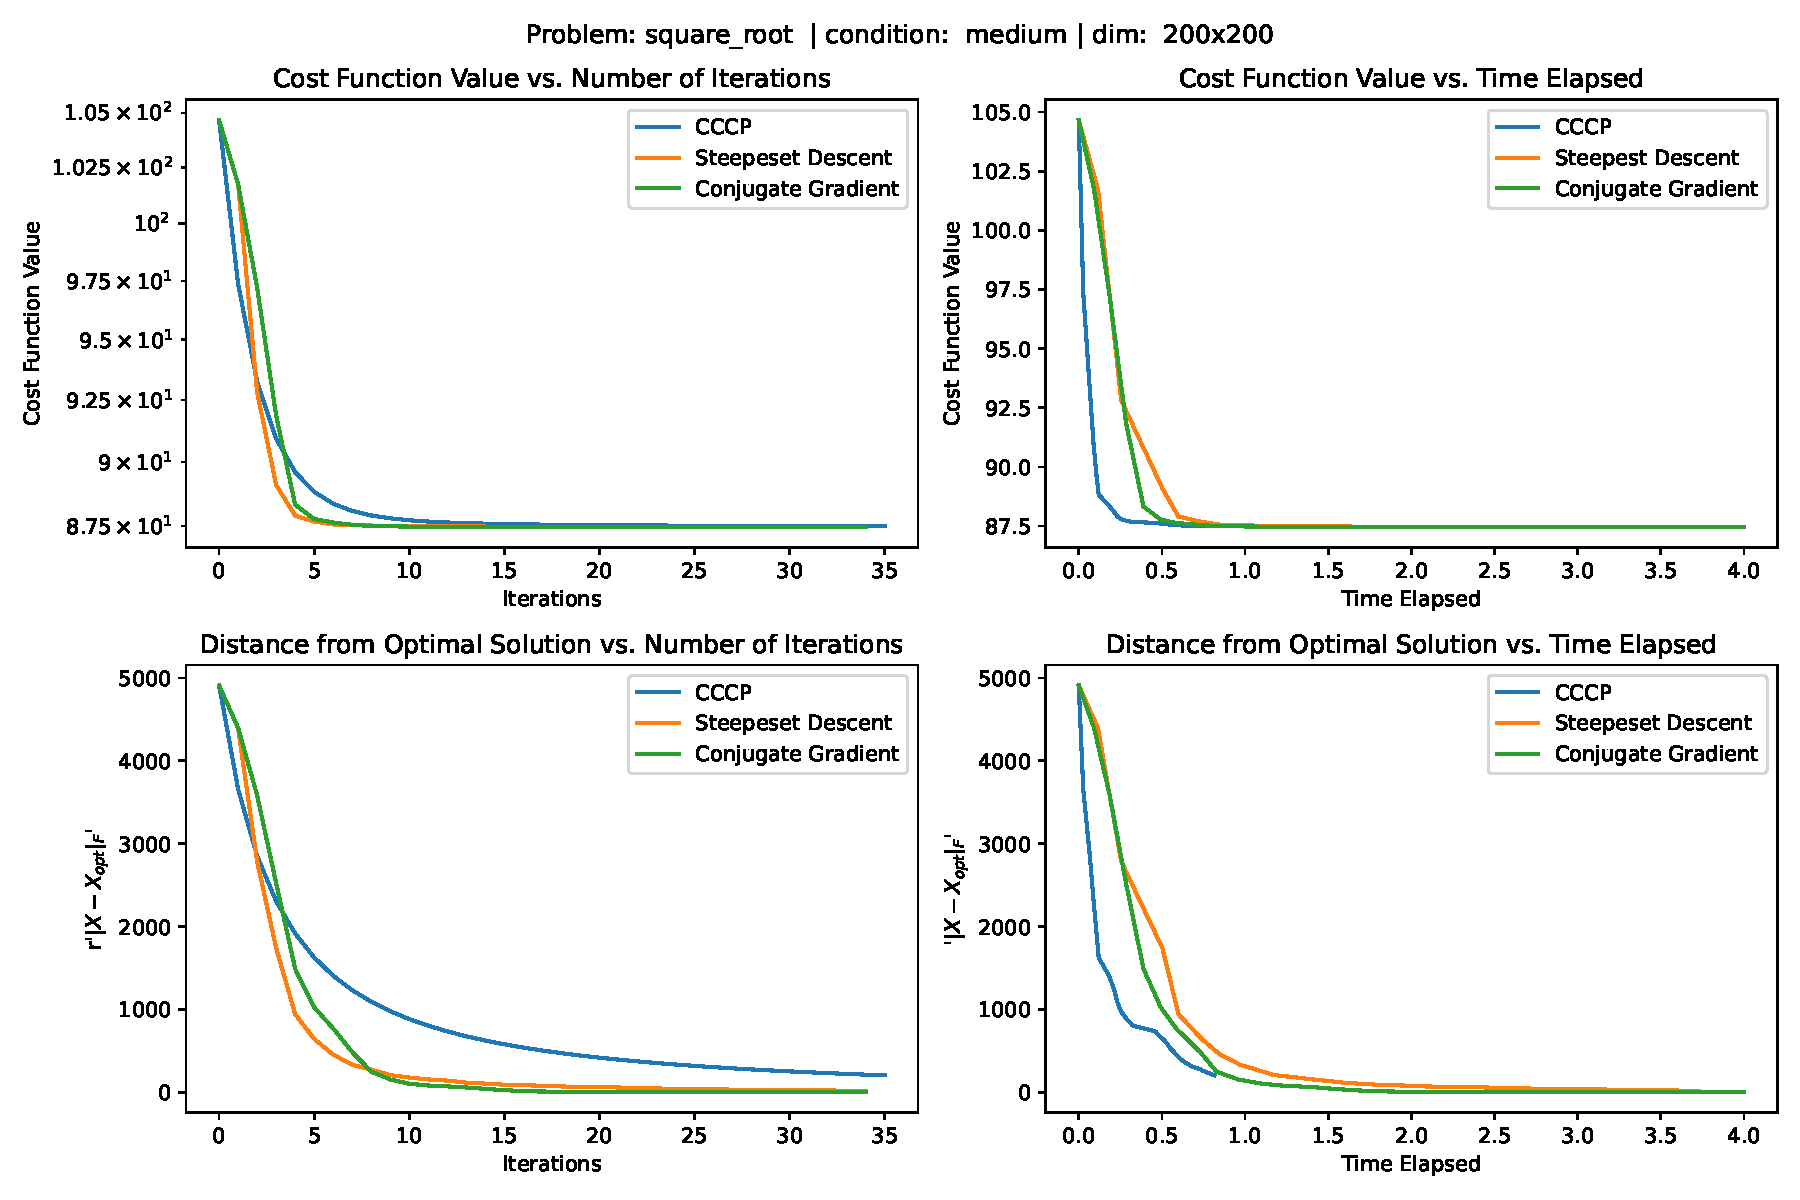
\includegraphics[height=10cm]{figures/square_root_medium_SDRGD_curves.pdf}
% 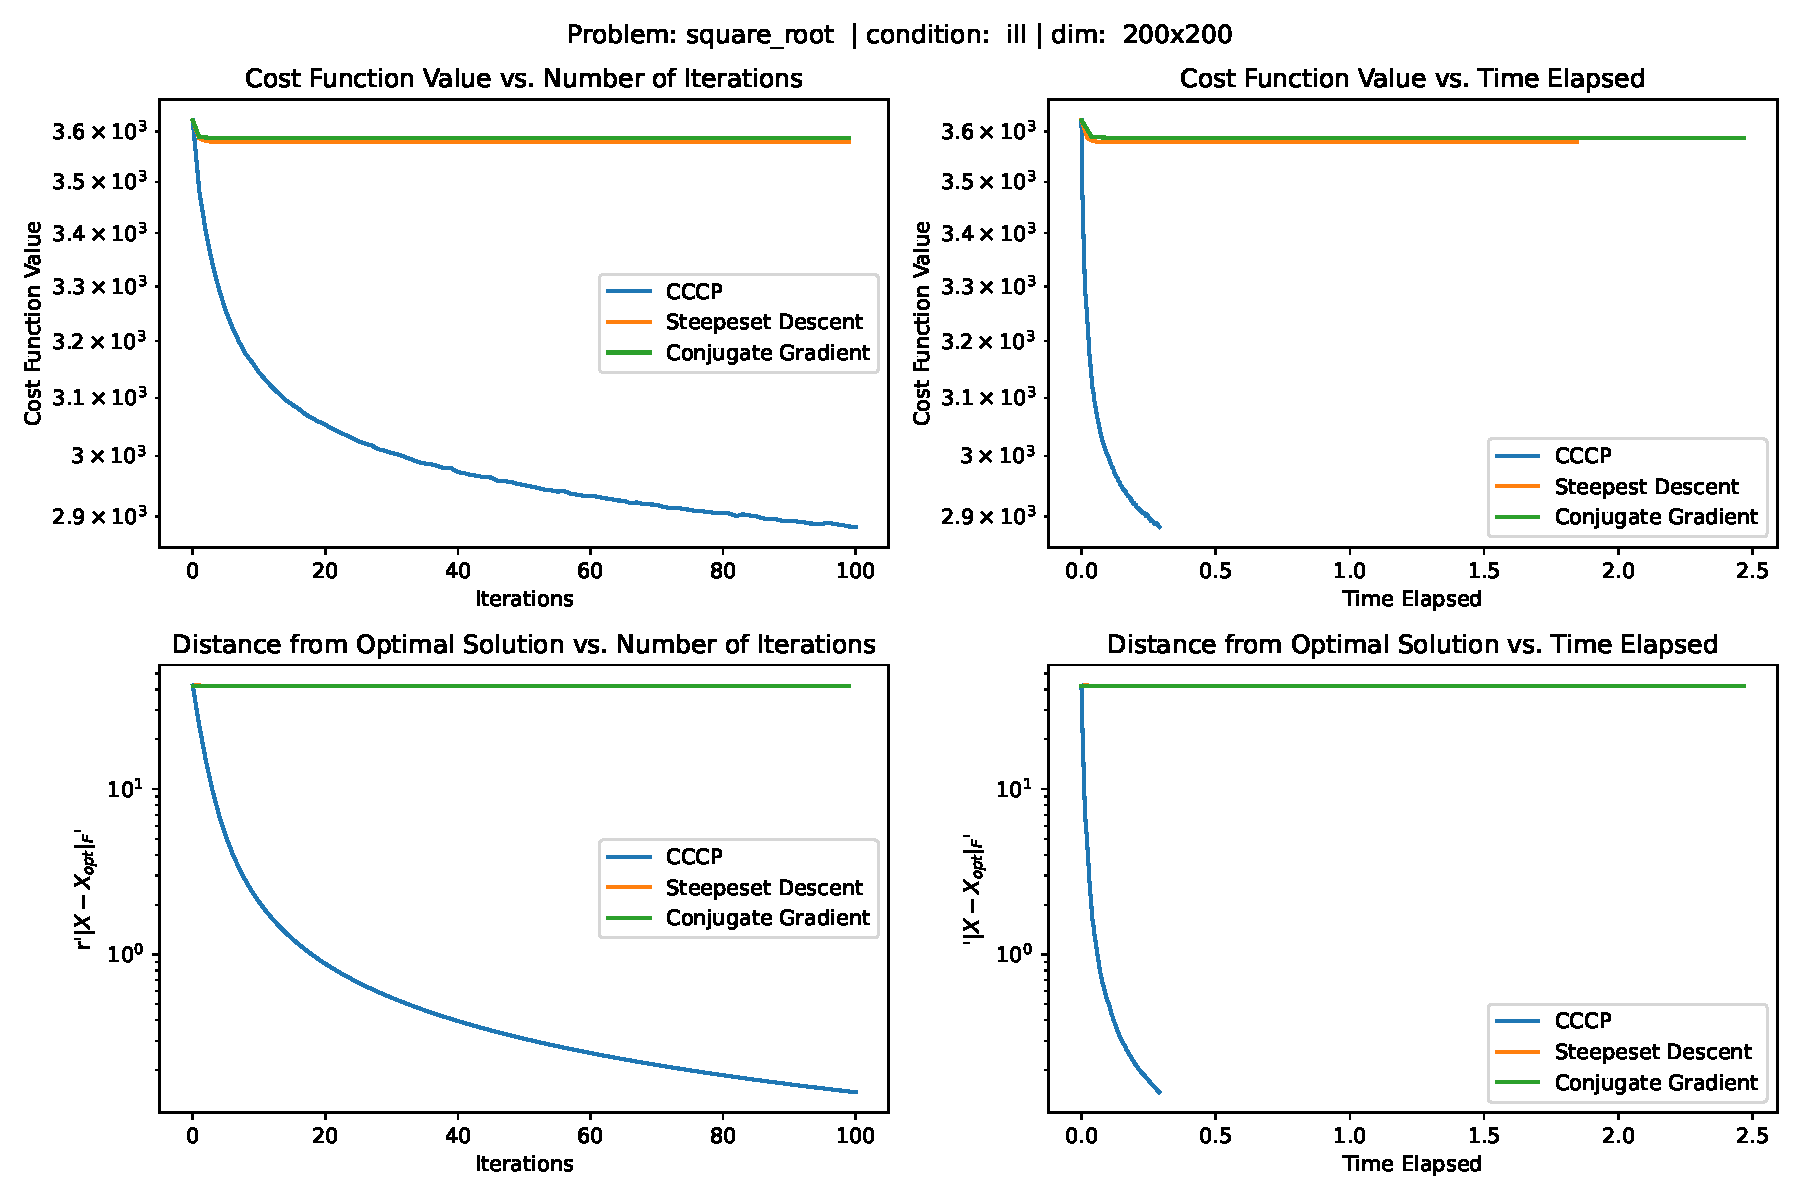
\includegraphics[height=10cm]{figures/square_root_ill_SDRGD_curves.pdf}
%     \caption{We apply the square root fixed-point algorithm (see Proposition~\ref{prop:fp_sqrt}) to the medium and ill-conditioned matrices where we took dimension $d=200$. In all cases, we initialized all algorithms at $X_0 = 3 I_d$. In the medium conditioned case we observe that all three methods perform comparatively in terms of iteration-complexity. The fixed-point method is superior in terms of runtime. Also, we observe that the fixed-point method is more robust to ill-conditioning. All experiments are averaged across 15 runs.}
%     \label{fig: square_root_exp}
% \end{figure}
% \begin{center}
    
% \end{center}



\paragraph{Gradient Steps}
The poor convergence of the Riemannian first-order methods holds across different very ill-conditioned matrices beyond the Hilbert matrix. For example, one can take the ill-conditioned linear low $k$-rank projections of $G G^\top$ with small perturbation $\delta I$ for $\delta \approx 0$. The first-order methods fail to converge for this ill-conditioned matrix as well.
In the following, we discuss this observation and a possible explanation on the example of the Hilbert matrix.
Recall that RGD preforms updates (for some stepsize $\eta > 0$)
\[
X \leftarrow \operatorname{Exp}(-\eta \operatorname{grad}\phi(X)) \; ,
\]
where the exponential map is defined as
\[
\operatorname{Exp}_X(t V)=X^{1 / 2} \exp \left(t X^{-1 / 2} V X^{-1 / 2}\right) X^{1 / 2}.
\]
Inserting this and the Riemannian gradient $\operatorname{grad}\phi(X)$ (see sec.~\ref{sec:background}) above gives
\[
\operatorname{Exp}(-\eta \operatorname{grad}\phi(X)) = X^{1/2} \exp \left(-\eta  X^{1/2} \nabla_X \Bar{\phi}(X) X^{1/2} \right)X^{1/2} 
\]
with
\[
\nabla \bar{\phi}(X) = \frac{1}{2}\left(\frac{X+A}{2}\right)^{-1} + \frac{1}{2}\left(\frac{X+I}{2}\right)^{-1} - X^{-1} \; .
\]
We suspect that computing the inverse of $X^{-1}$, i.e., inverting the Hilbert matrix at each iteration of the first-order methods results in numerical instability leading to the exhibited poor convergence behaviour. 
In contrast, the CCCP approach (Eq.~\ref{eq:sqrt_fp}) is robust to ill-conditioned matrices. Adding the identity $X+I$ improves the condition number of $X$ before taking inverses. Although $X+A$ does not have better conditioning than $A$ in general, we observe that in cases where $A$ is ill-conditioned, the matrix $X+A$ actually becomes well-conditioned in practice. Heuristically, this follows from Weyl's inequality which implies 
    \[
    \kappa(A+B) \leq \frac{\lambda_{\max}(A) + \lambda_{\max}(B)}{\lambda_{\min}(A) + \lambda_{\min}(B)} \qquad \text{for} \qquad A,B \in \pd \; ,
    \]
    where $\kappa(X)$ is the condition number of $X.$ This is demonstrated in Figure~\ref{fig:cond_num_sqrt}.
%
\begin{figure}[ht]
  \centering
  \begin{minipage}[b]{0.45\textwidth}
    \centering
    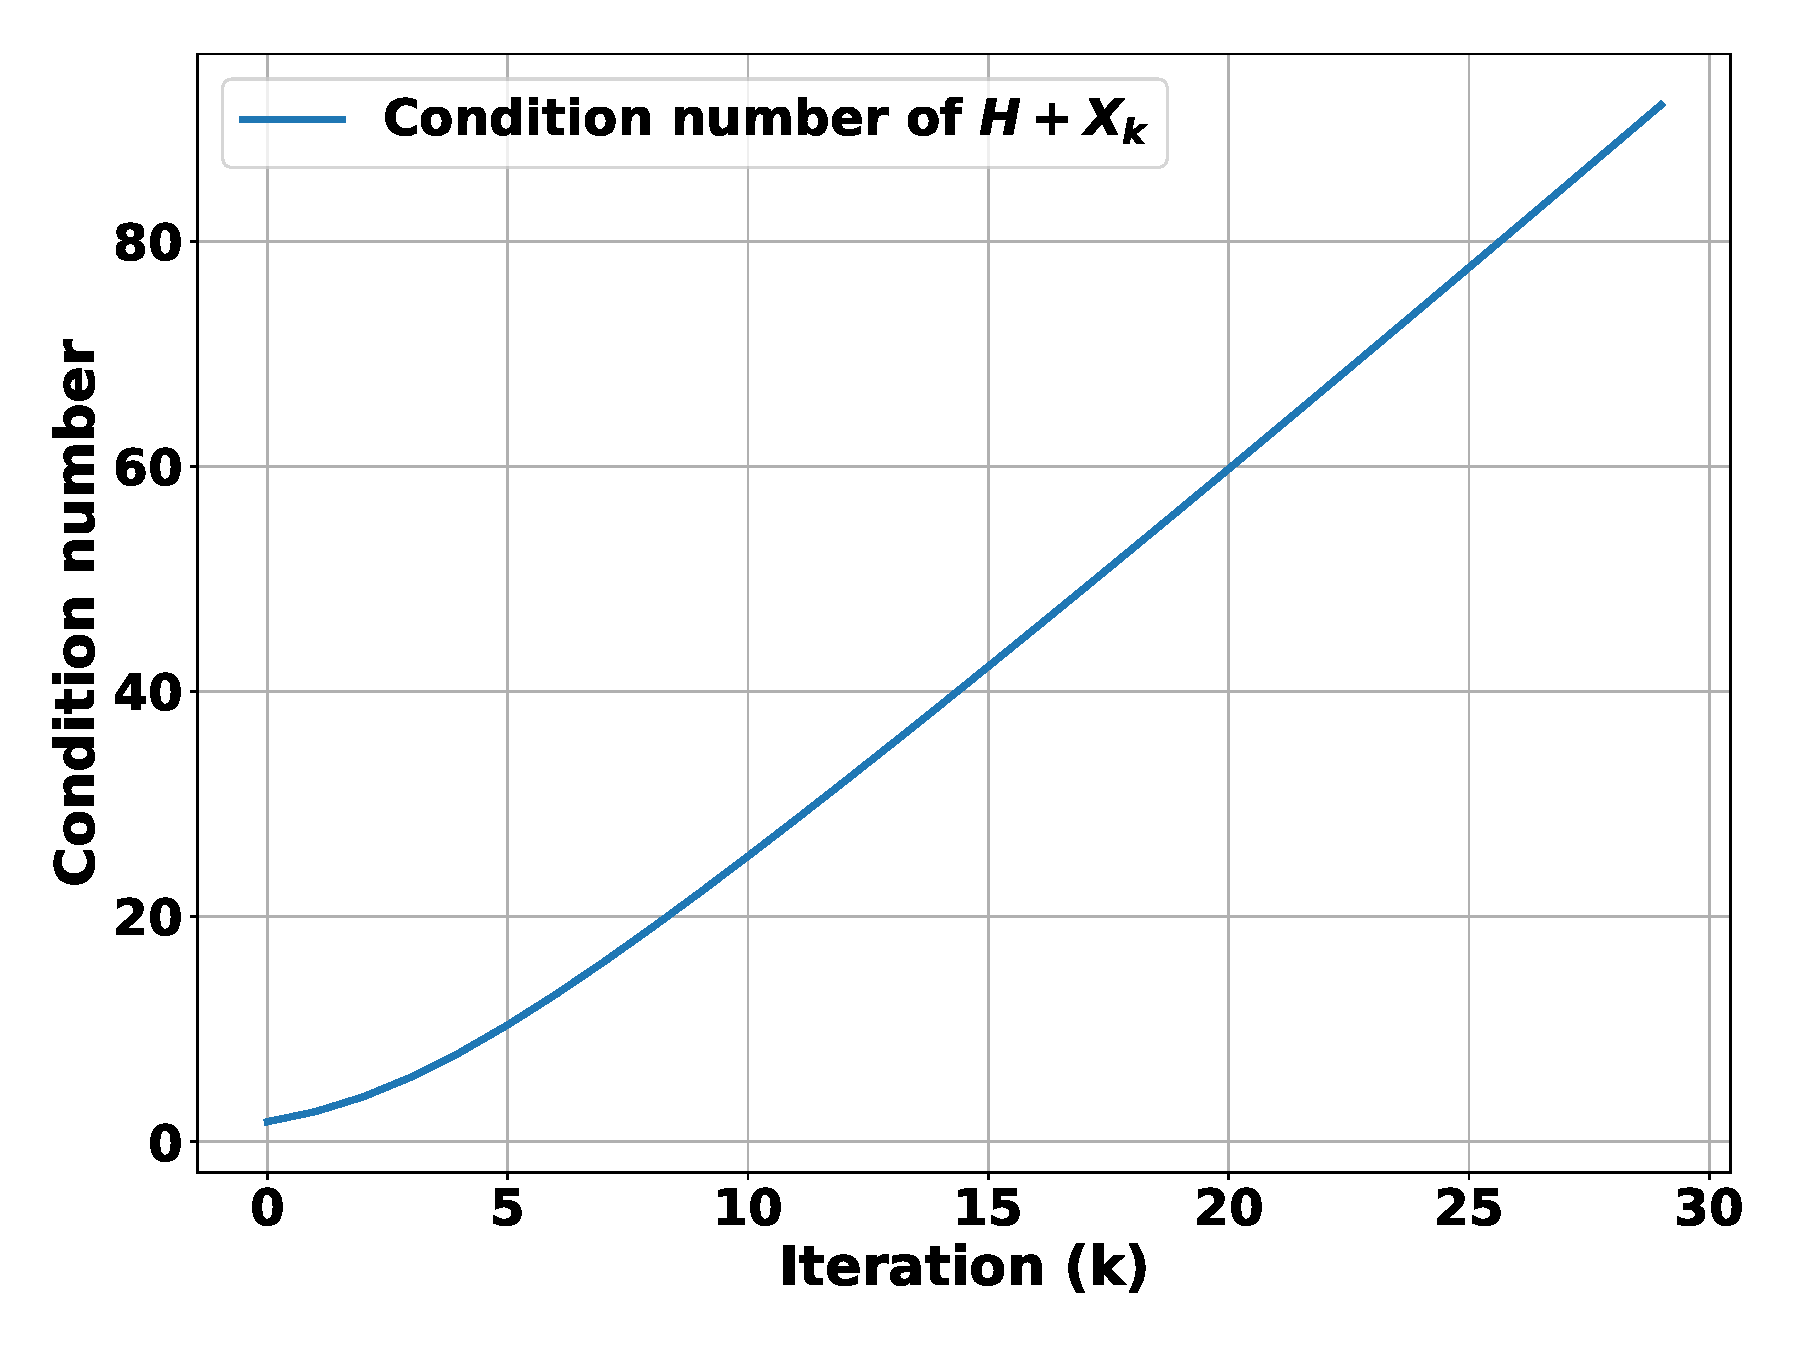
\includegraphics[width=\textwidth]{figures/A_rankK.pdf}
  \end{minipage}
  \hfill
  \begin{minipage}[b]{0.45\textwidth}
    \centering
    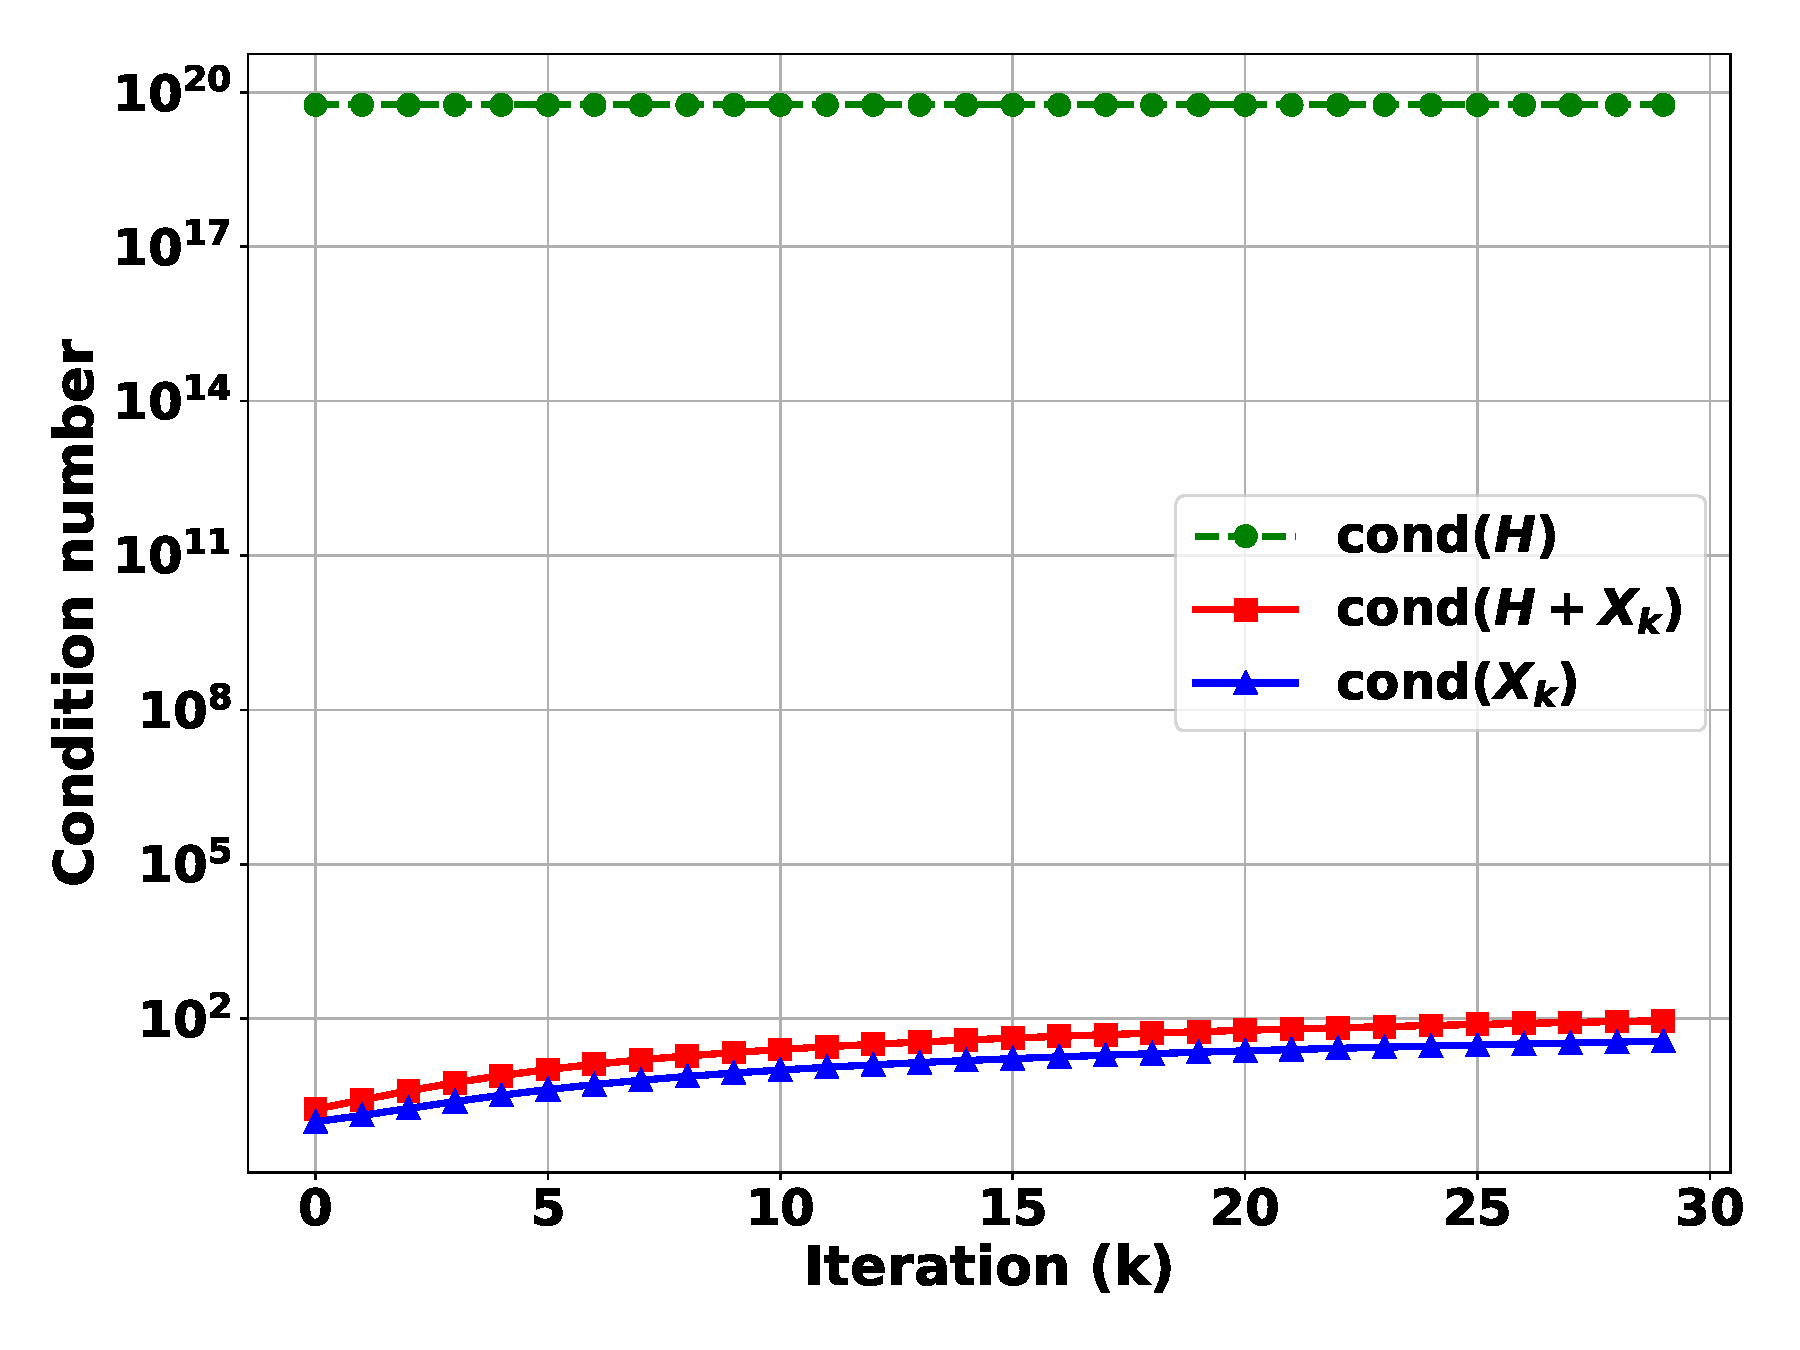
\includegraphics[width=\textwidth]{figures/A_X_rankK.pdf}
  \end{minipage}
  \caption{We generate the Hilbert matrix $H \in \mathbb{R}^{200 \times 200}$. We plot the condition number of $H+X_k$ where $X_k$ is the $k$-th iterate of the fixed-point algorithm~\ref{eq:sqrt_fp} and compare this to the condition number of $H$. Clearly, $H+X_k$ is much better conditioned than $H$. This trend also holds for other very ill-conditioned matrices.}
  \label{fig:cond_num_sqrt}
\end{figure}



\subsection{Karcher Mean}
In this section, we compare the performance of the CCCP approach, i.e., the fixed point approach given by Eq.~\ref{eq:karcher_fp}, to RGD and RCG for the Karcher mean problem (Eq.~\ref{problem:sdiv_karcher_mean}).

% we have three settings: well-conditioned, medium-conditioned, and ill-conditioned. 

\paragraph{Data generation} 
% In the \textit{well-conditioned} case, we construct the data $\{A_k: k \in [m]\}$ as follows. We sample \textit{m} number of $d \times d$ matrices $U^{(k)}$ whose entries are i.i.d distributed as $U^{(k)}_{ij} \in \mathcal{U}(0,1)$. Then we construct $A_k \defas U^{(k)}U^{(k)\top}$.
We focus on the medium-conditioned case, where we sample $G_{1}, \ldots, G_m $ random matrices, each with i.i.d standard Gaussian entries, and construct the data points $A_k \defas G_kG_k^\top$. A proxy for the true optimum is obtained by averaging the last iterate of the three algorithms upon convergence.


\paragraph{Results}
Figures~\ref{fig:karcher_mean_100_100} and~\ref{fig:karche_mean_100_500} show the convergence of all three algorithms.
We see that the CCCP algorithm exhibits superior runtime  compared to the two Riemannian first-order methods. Notably, the gap between CCCP and the two gradient-based approaches only widens as we increase the dimensionality and number of data samples.

\begin{figure}[htbp]
  \centering
  \begin{minipage}[b]{0.45\textwidth}
    \centering
    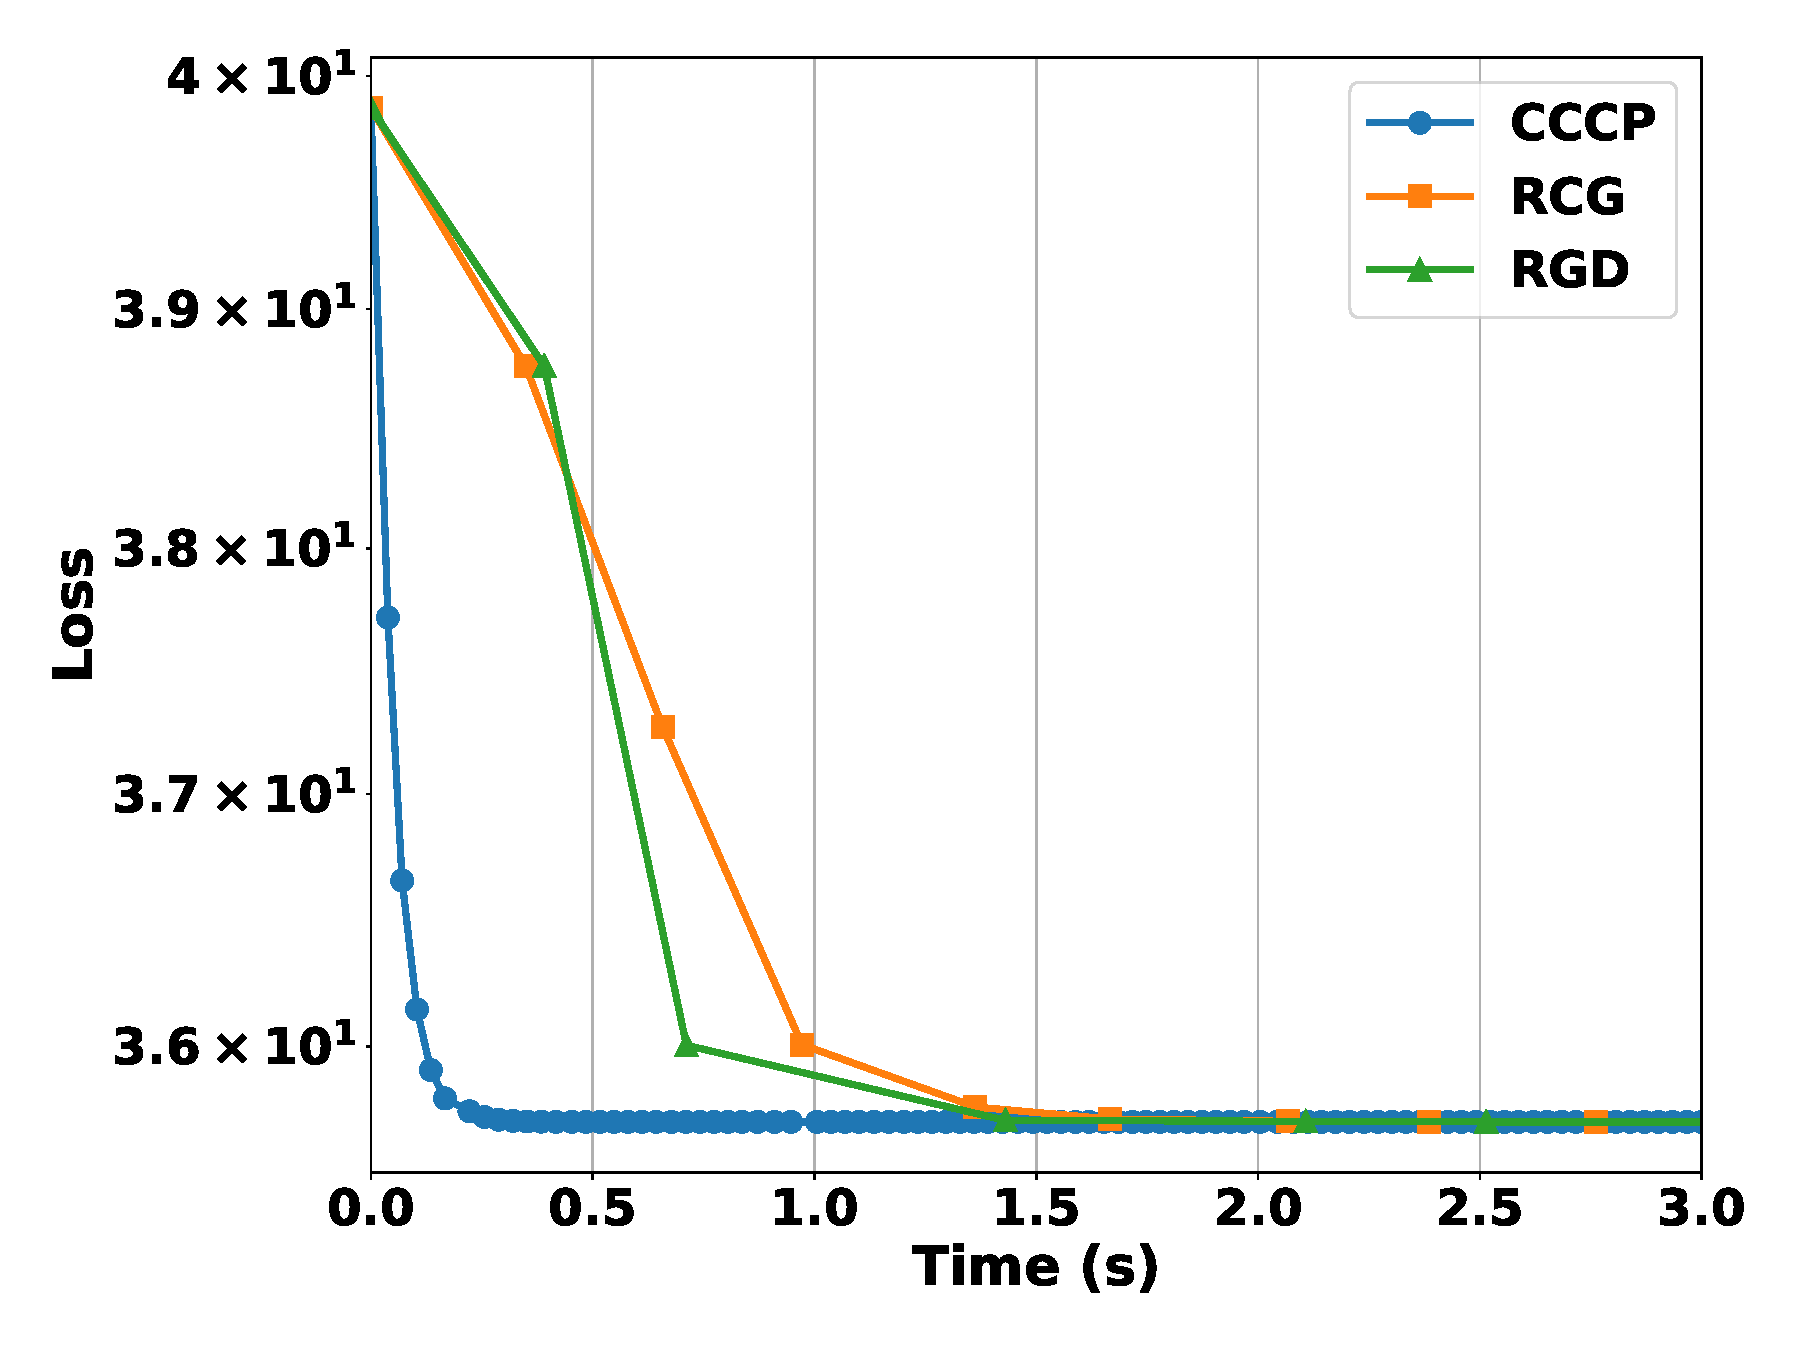
\includegraphics[width=\textwidth]{figuresV2/karcher_mean/loss_time_100_100_medium.pdf}
  \end{minipage}
  \hfill
  \begin{minipage}[b]{0.45\textwidth}
    \centering
    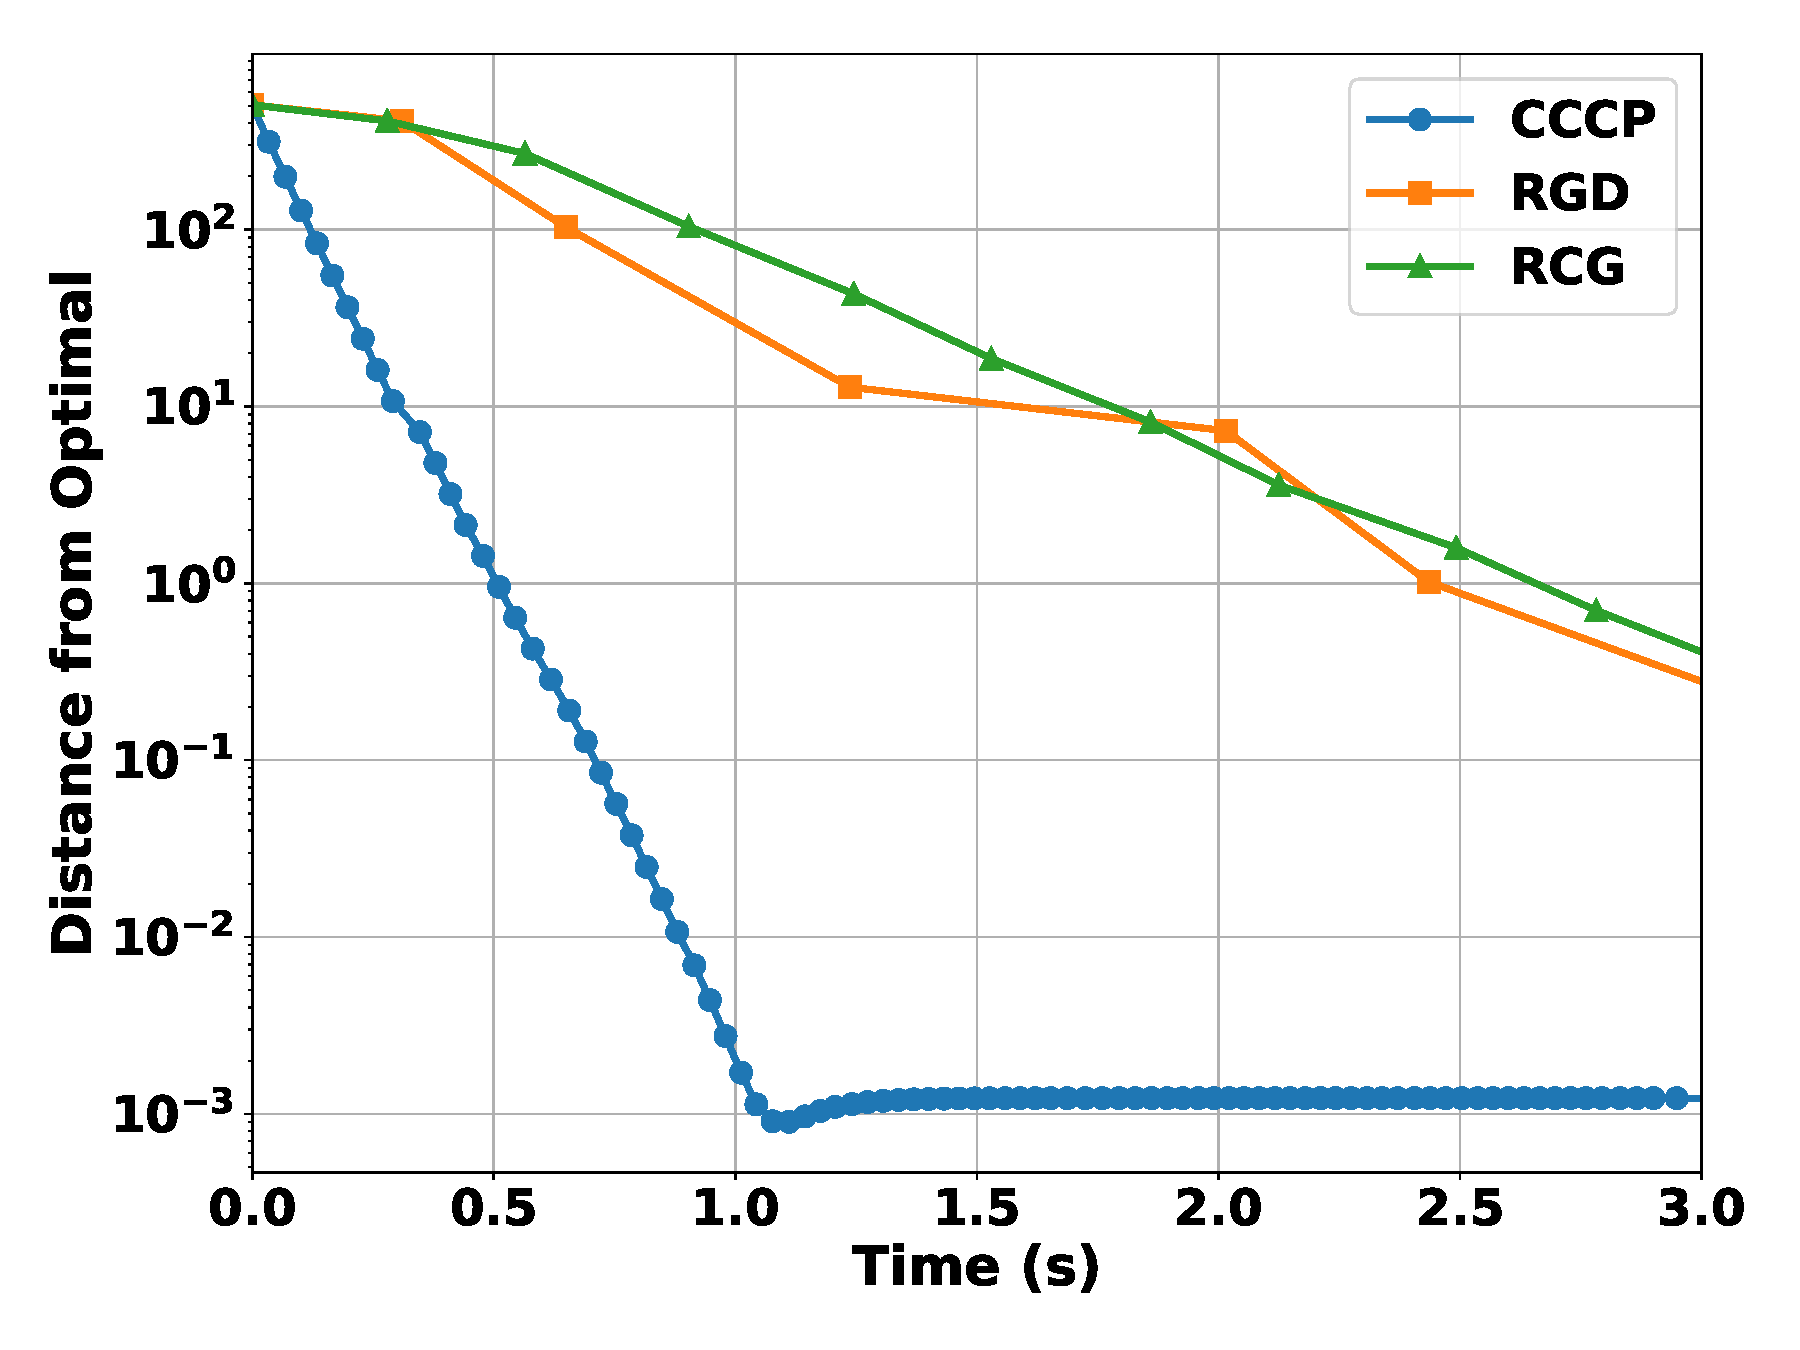
\includegraphics[width=\textwidth]{figuresV2/karcher_mean/distance_time_100_100_medium.pdf}
  \end{minipage}
  \caption{\textbf{Karcher Mean.} $m=100$ and $d=100$. . CCCP demonstrates superior runtime complexity.}
  \label{fig:karcher_mean_100_100}
\end{figure}

\begin{figure}[htbp]
  \centering
  \begin{minipage}[b]{0.45\textwidth}
    \centering
    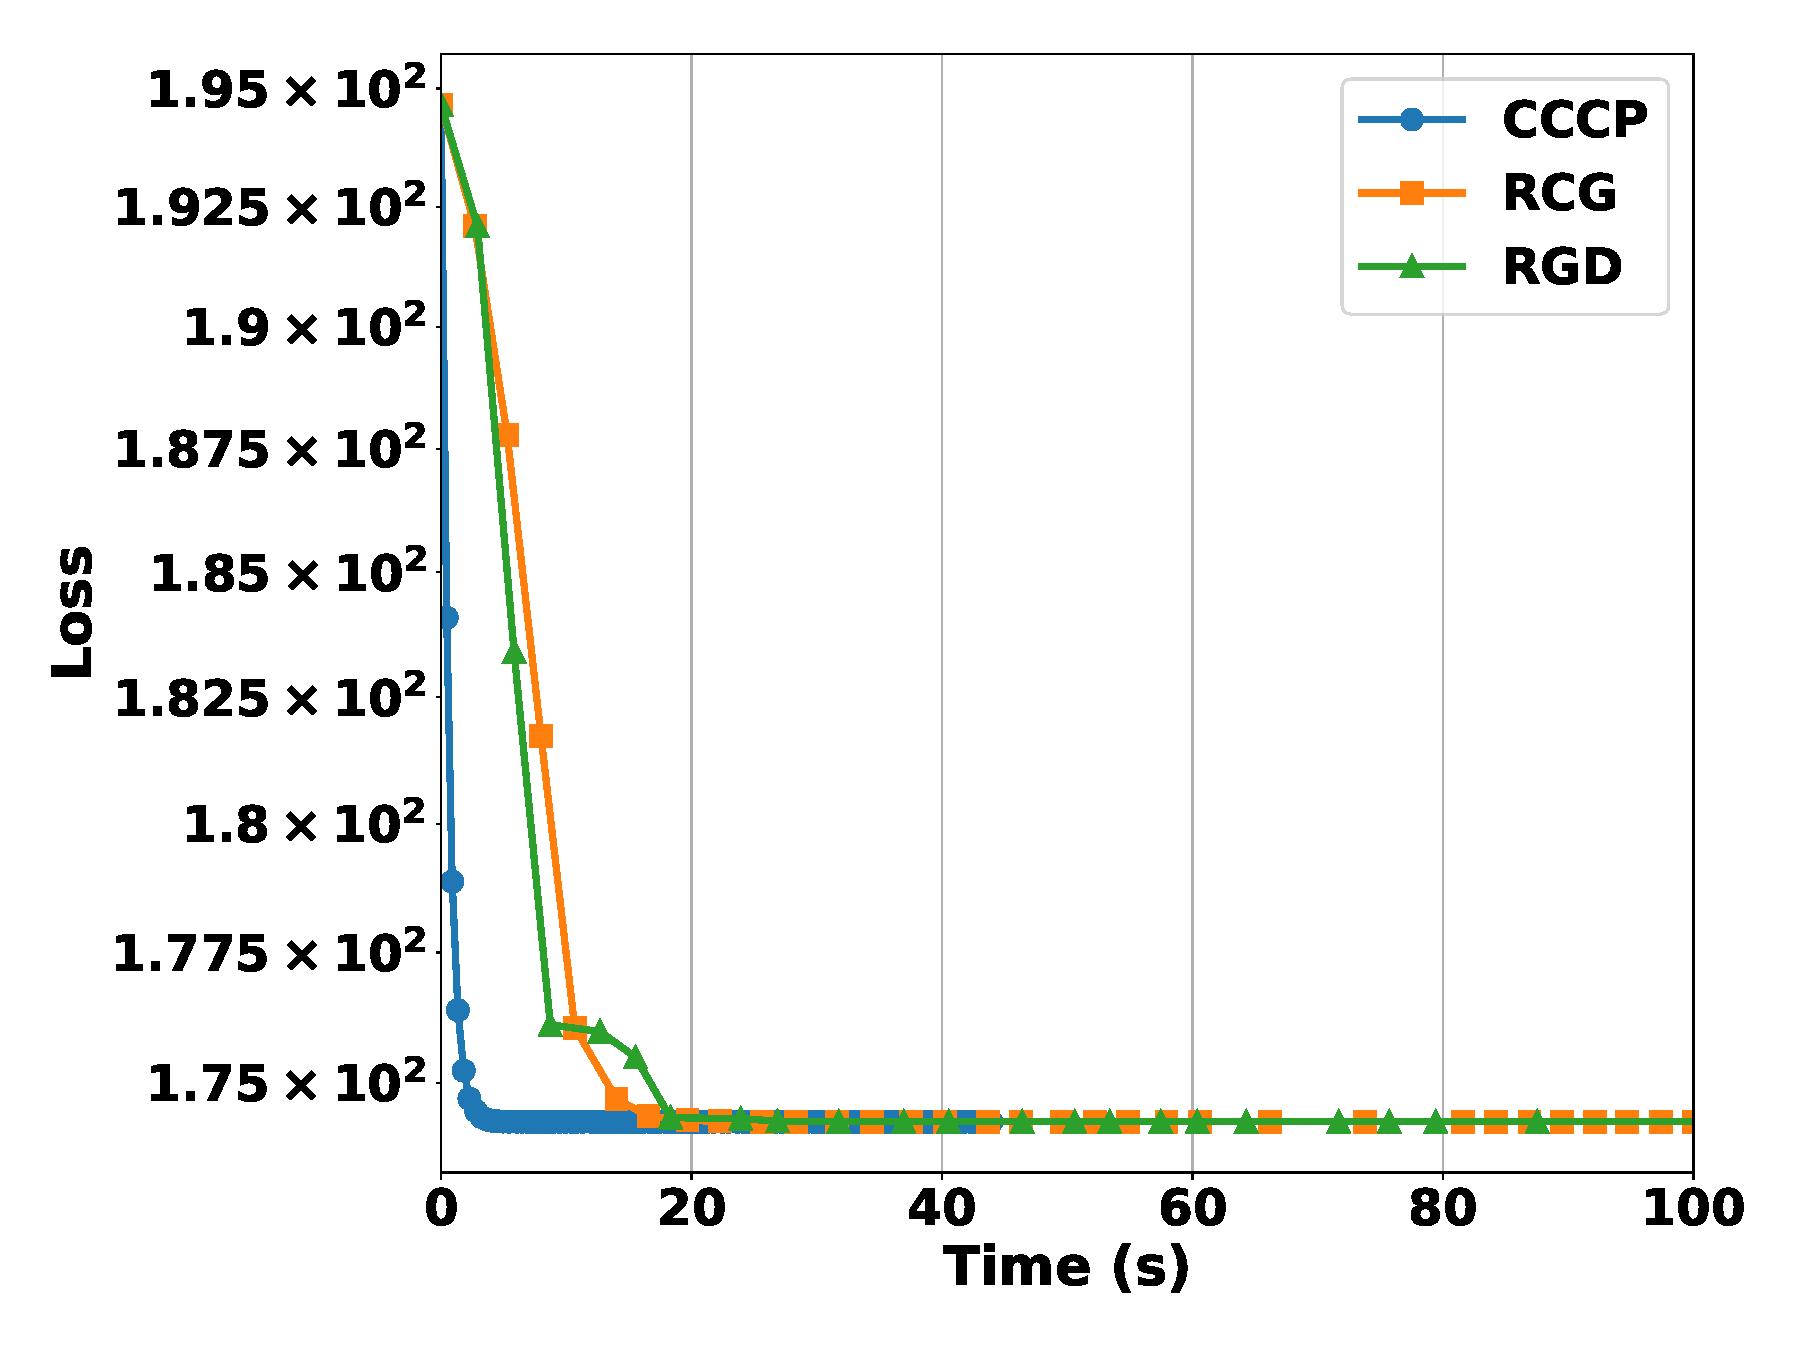
\includegraphics[width=\textwidth]{figuresV2/karcher_mean/loss_time_100_500_medium.pdf}
  \end{minipage}
  \hfill
  \begin{minipage}[b]{0.45\textwidth}
    \centering
    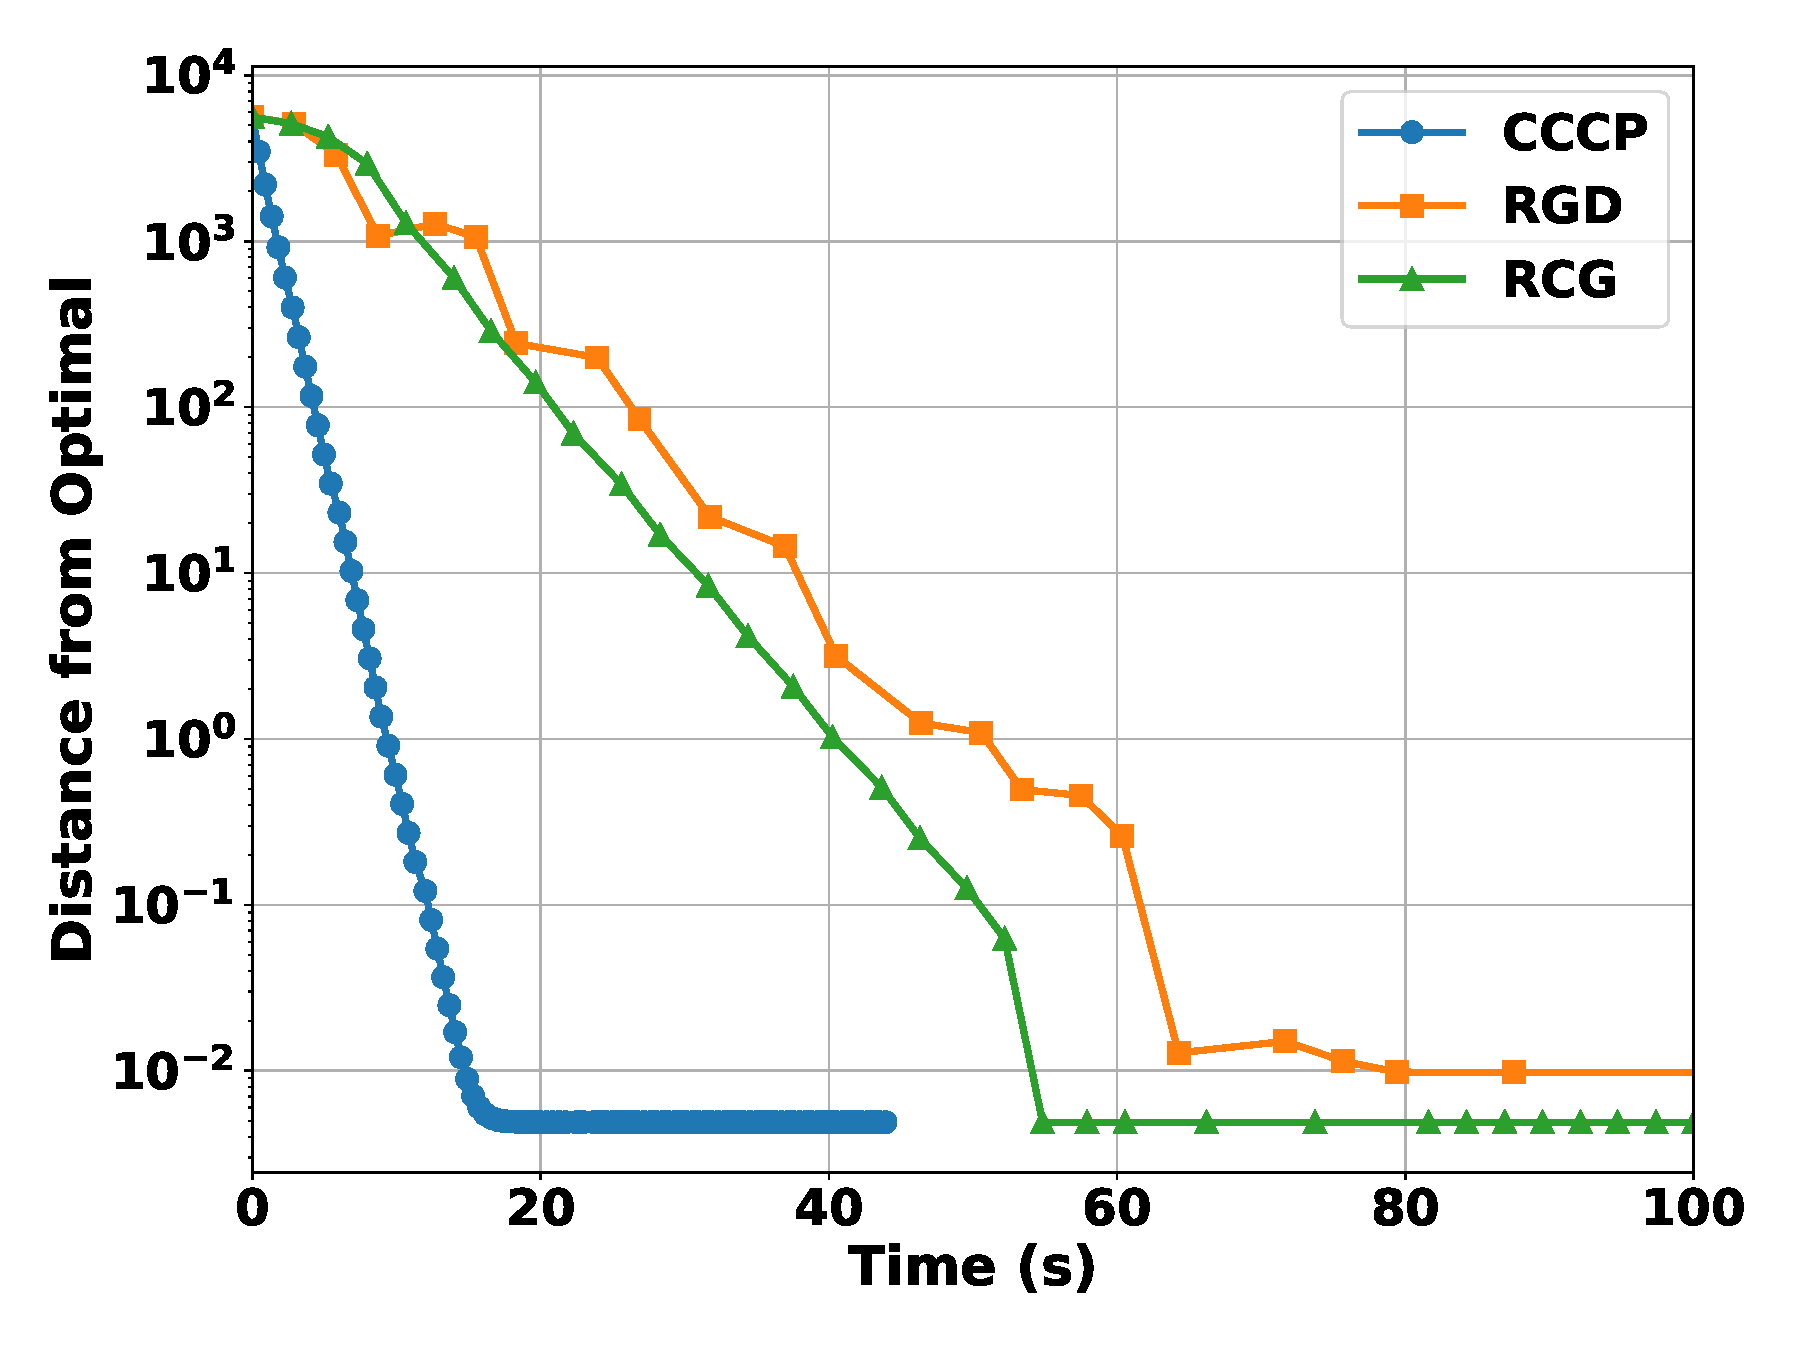
\includegraphics[width=\textwidth]{figuresV2/karcher_mean/distance_time_100_500_medium.pdf}
  \end{minipage}
  \caption{\textbf{Karcher Mean.} $m=100$ and $d=500$. We observe that the gap between the runtime performance between CCCP and the benchmarks widens as we take the dimension $d$ to be larger.}
  \label{fig:karche_mean_100_500}
\end{figure}





% \begin{figure}
%     \centering
%     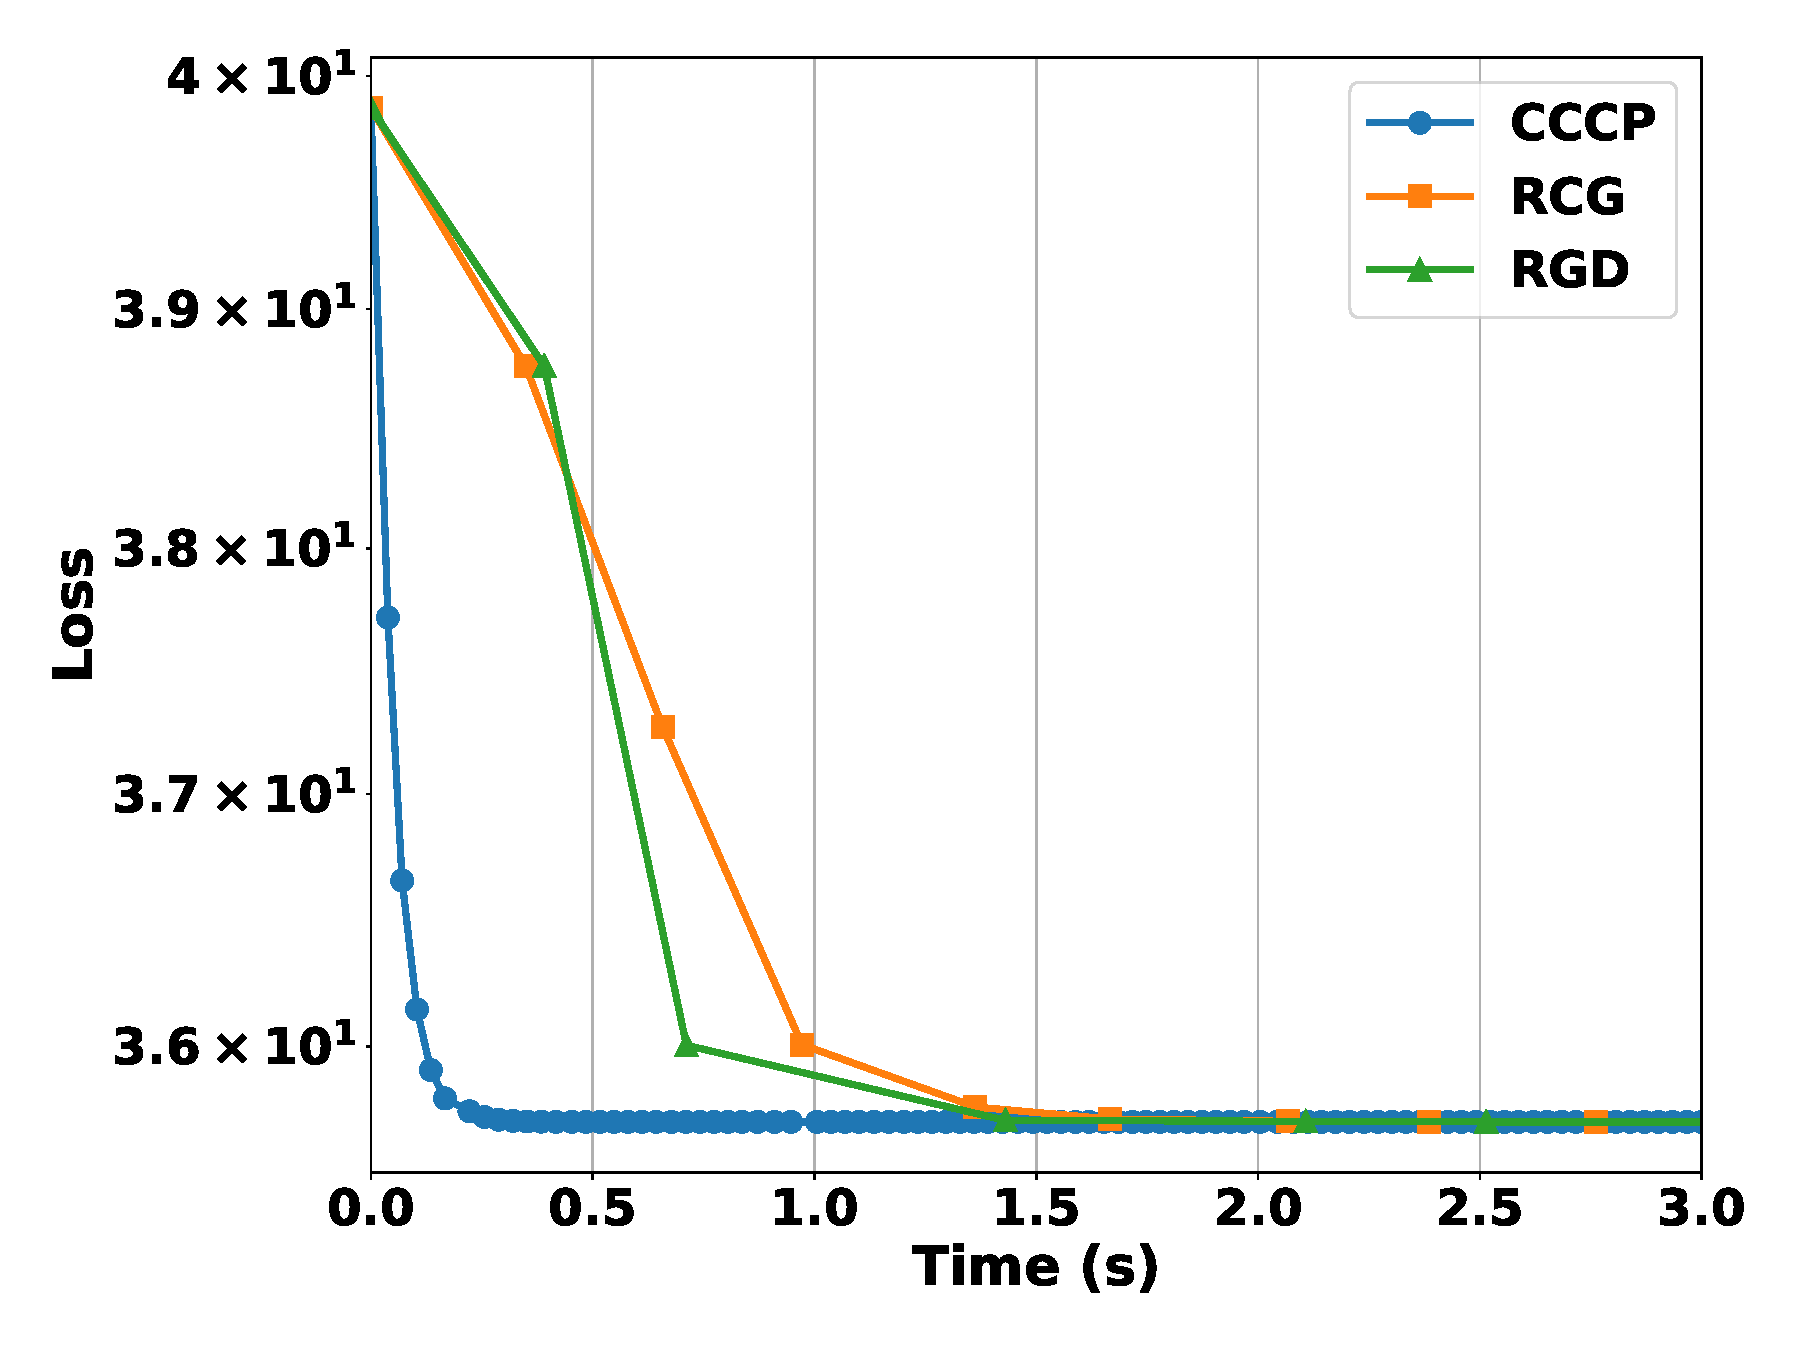
\includegraphics[height=6.1cm]{figuresV2/karcher_mean/loss_time_100_100_medium.pdf}
%     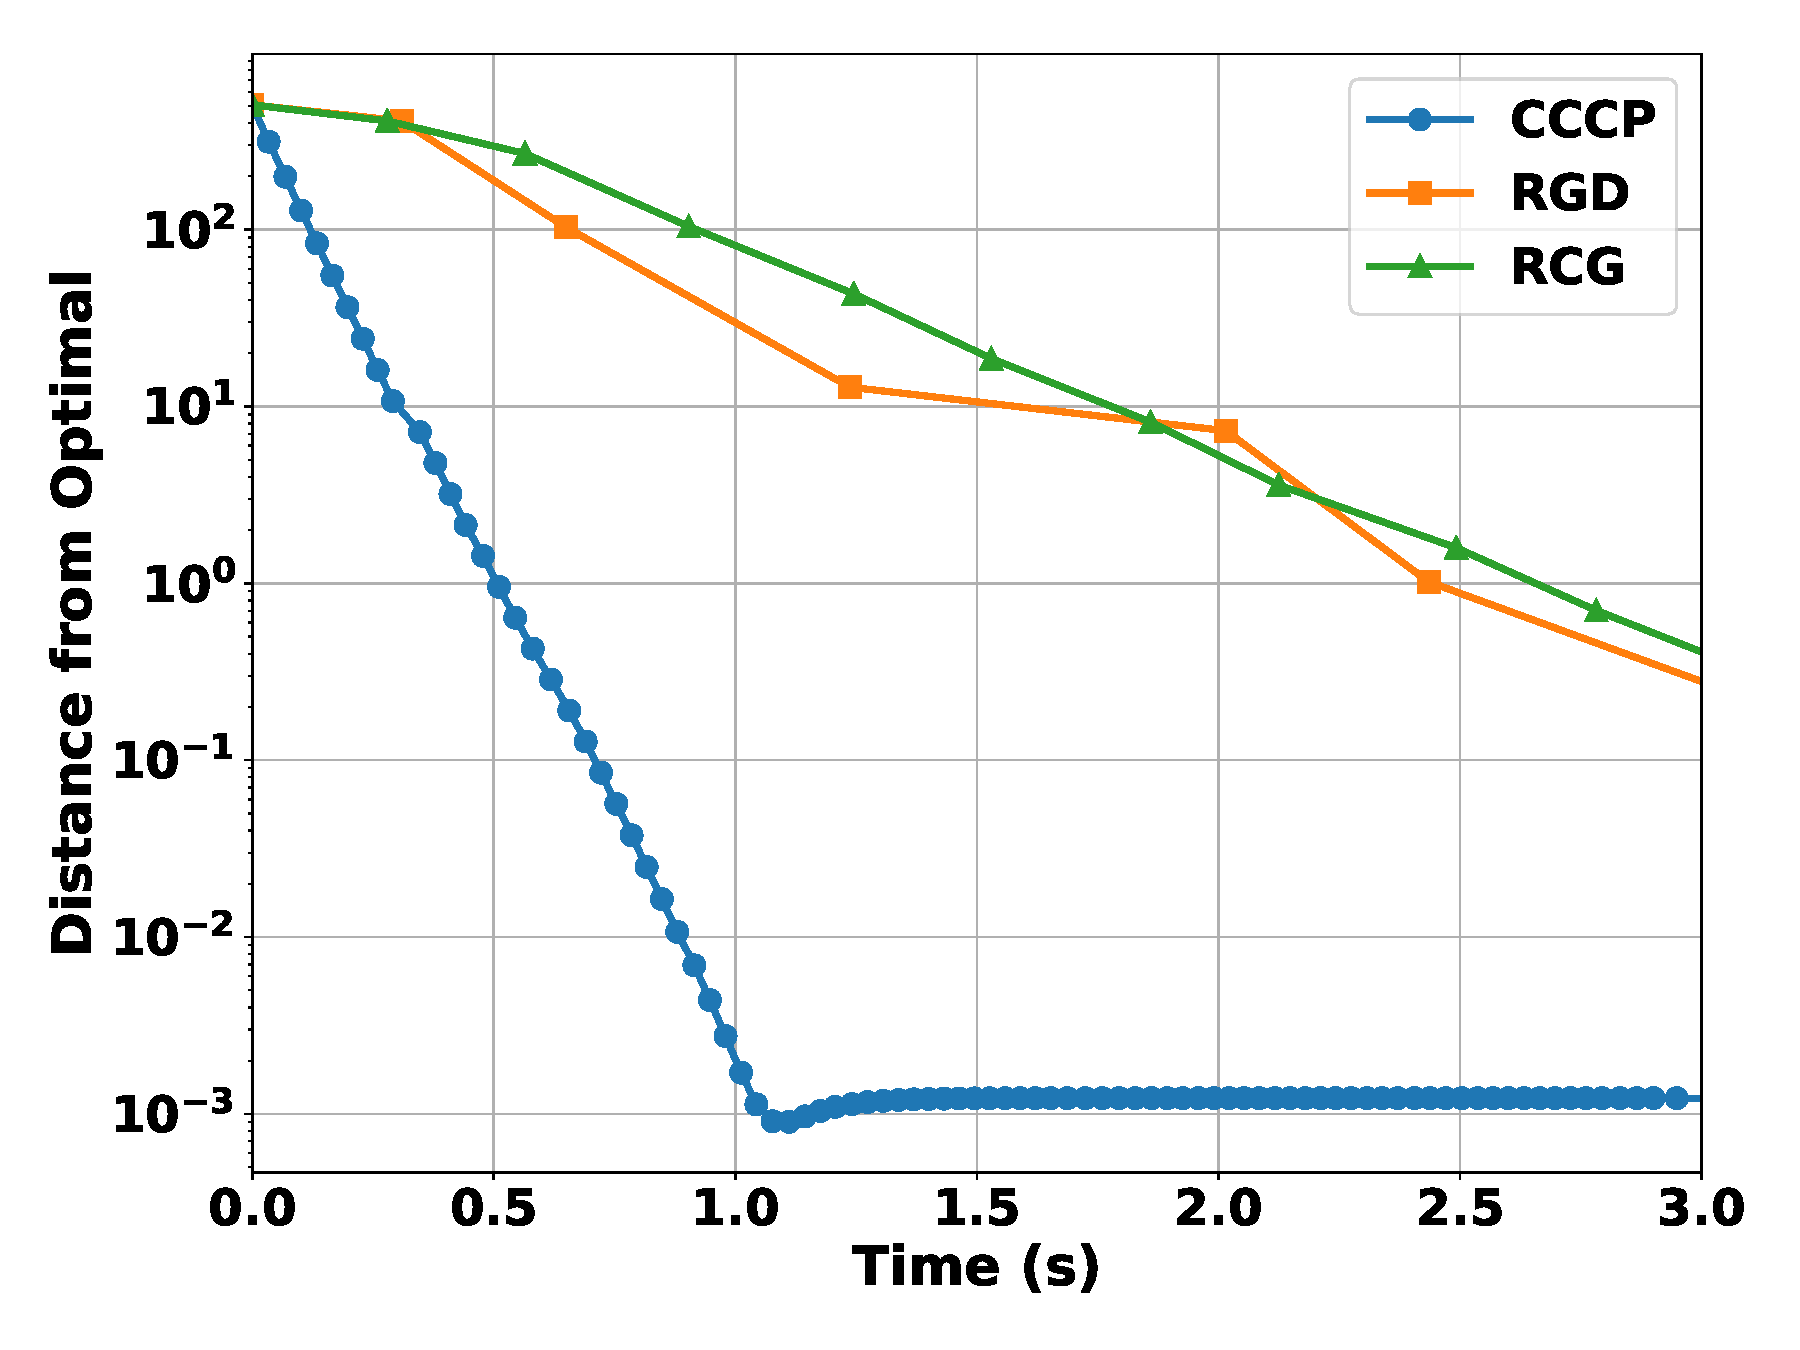
\includegraphics[height=6.1cm]{figuresV2/karcher_mean/distance_time_100_100_medium.pdf}
%     \caption{\textbf{Karcher Mean.} $m=100$ and $100 \times 100$ matrices. We observe that all algorithms exhibit comparative iteration complexity. CCCP demonstrates superior runtime complexity. {\color{red}TODO Andrew: typo "steepest descent" -- please correct}}
%     \label{fig:karcher_mean_100_100}
% \end{figure}

\begin{figure}[htbp]
  \centering
  \begin{minipage}[b]{0.45\textwidth}
    \centering
    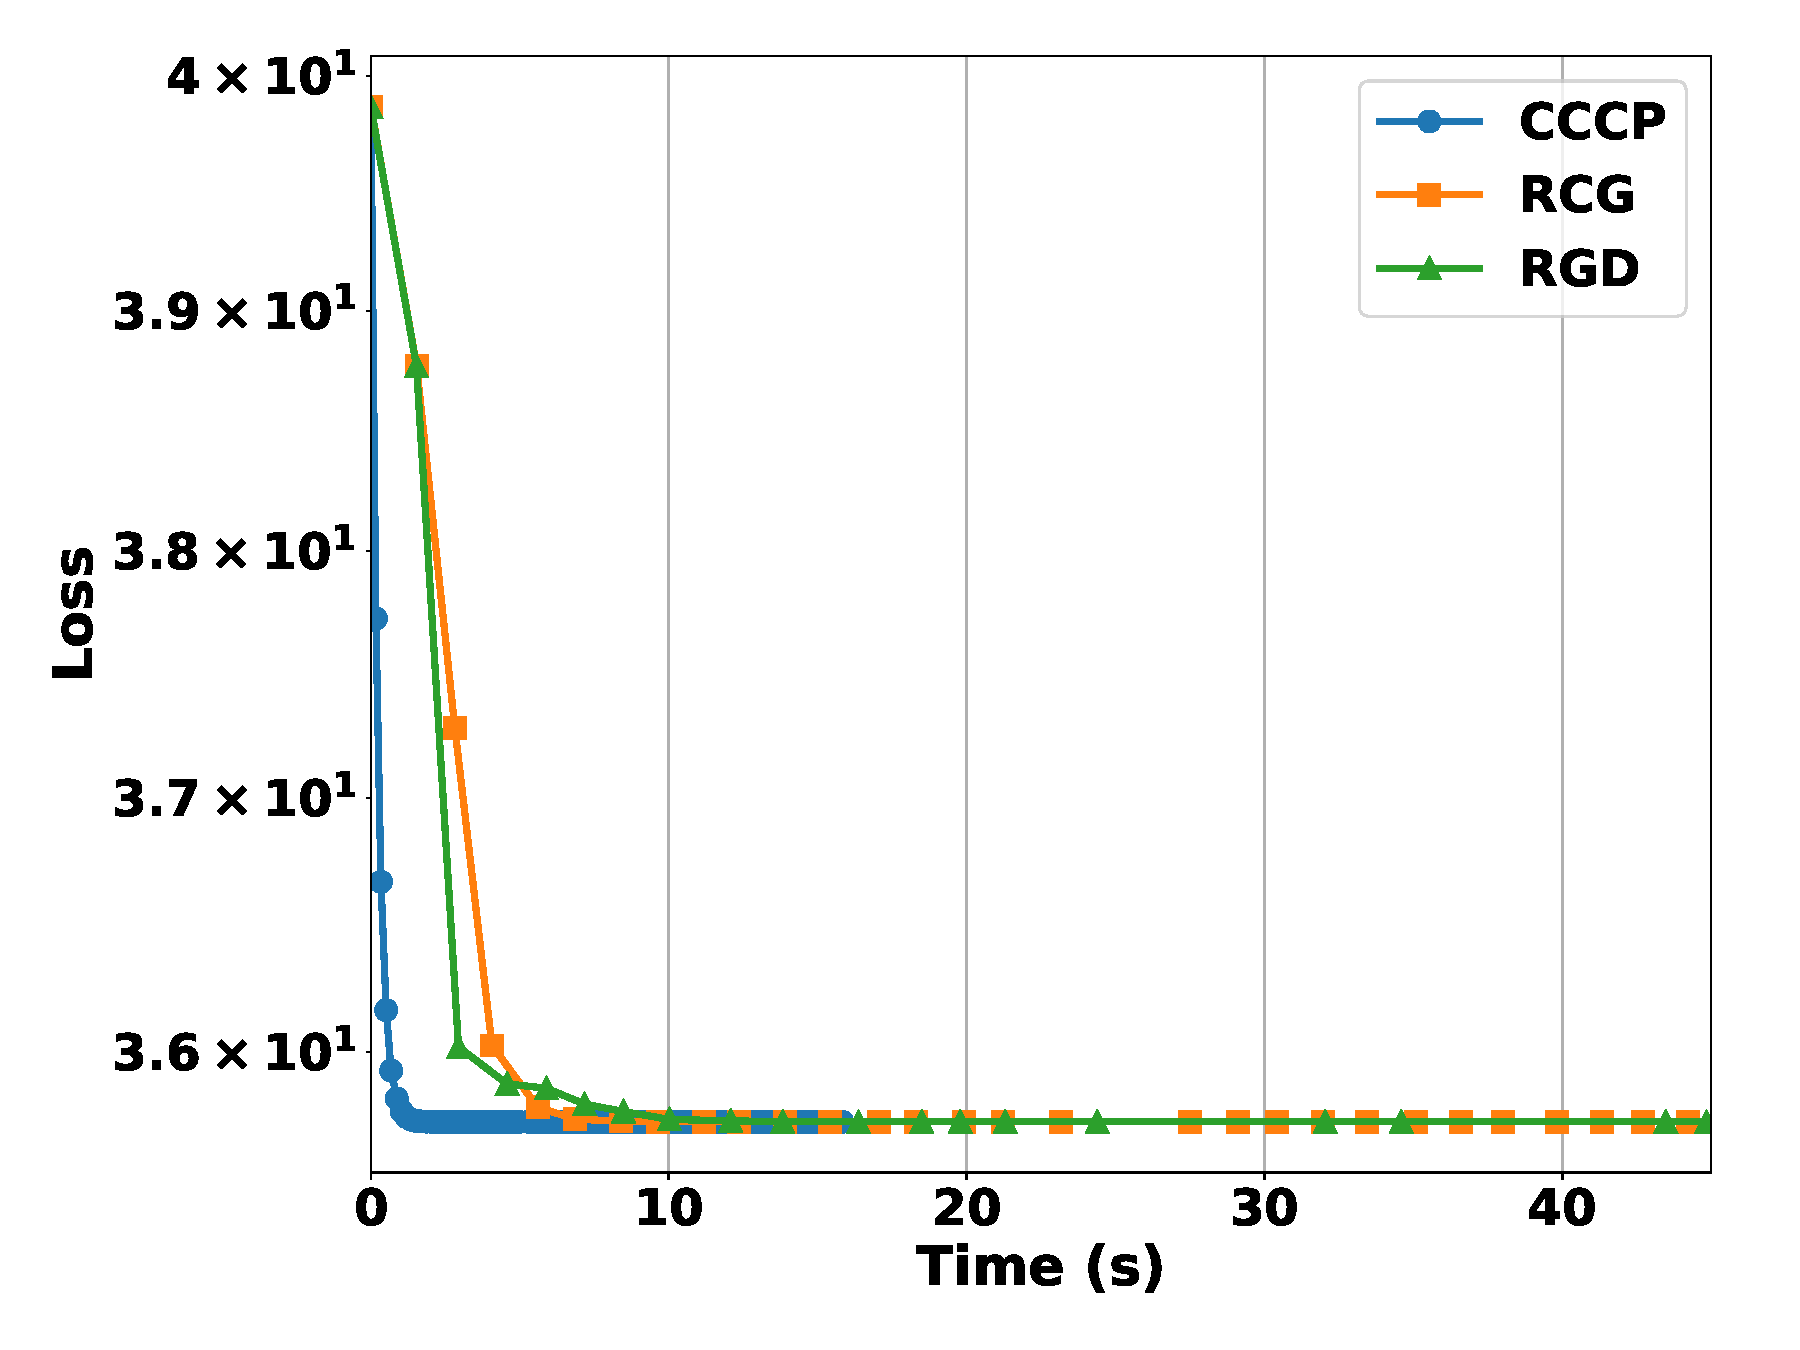
\includegraphics[width=\textwidth]{figuresV2/karcher_mean/loss_time_500_100_medium.pdf}
  \end{minipage}
  \hfill
  \begin{minipage}[b]{0.45\textwidth}
    \centering
    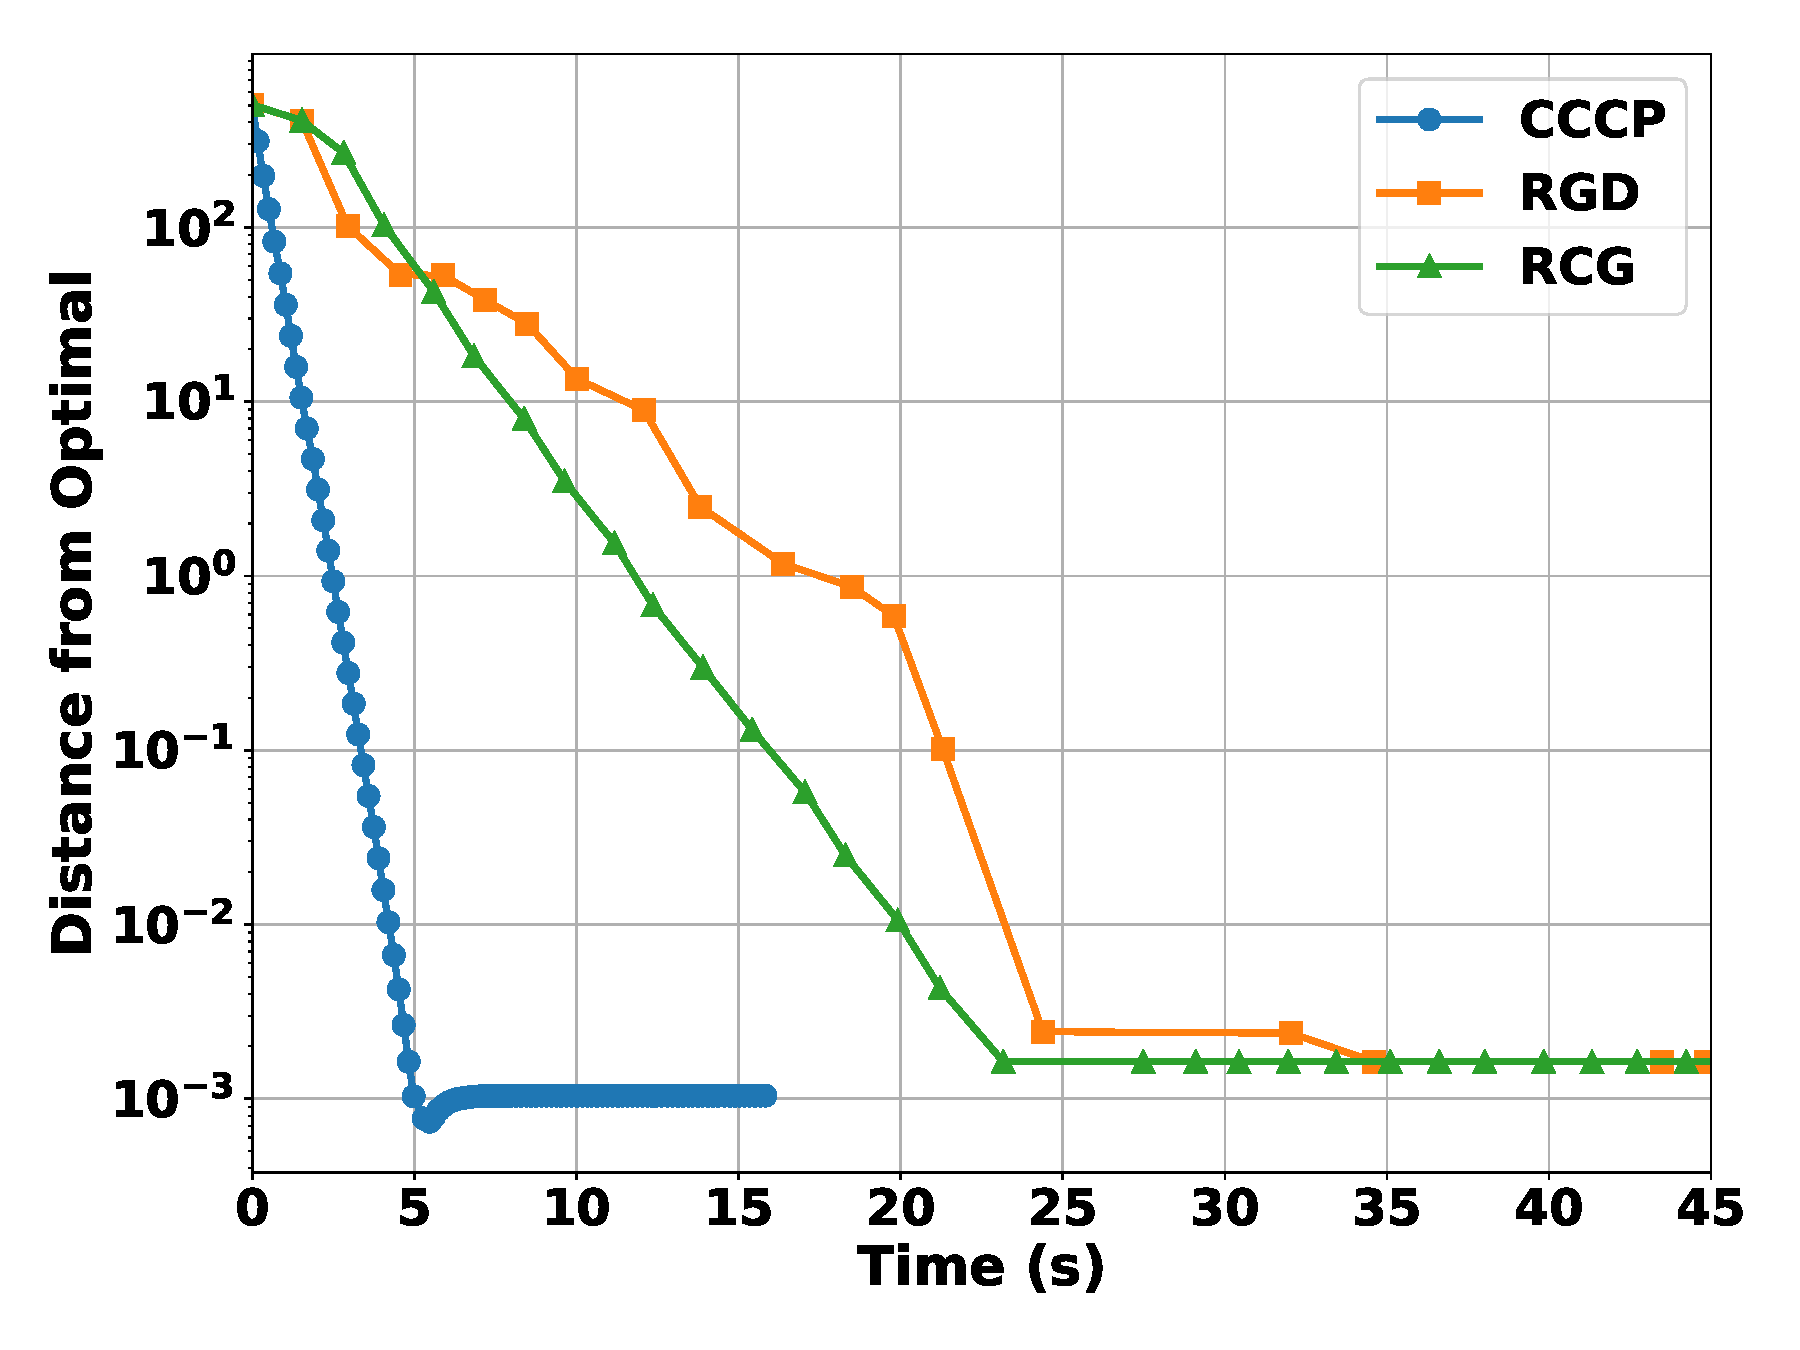
\includegraphics[width=\textwidth]{figuresV2/karcher_mean/distance_time_500_100_medium.pdf}
  \end{minipage}
  \caption{\textbf{Karcher Mean.} $m=500$ and $d=100$. We observe that the gap between the runtime performance between CCCP and the benchmarks widens as we take the number of samples $m$ to be larger.}
  \label{fig:karcher_mean_500_100}
\end{figure}


% \begin{figure}[ht]
%     \centering
%      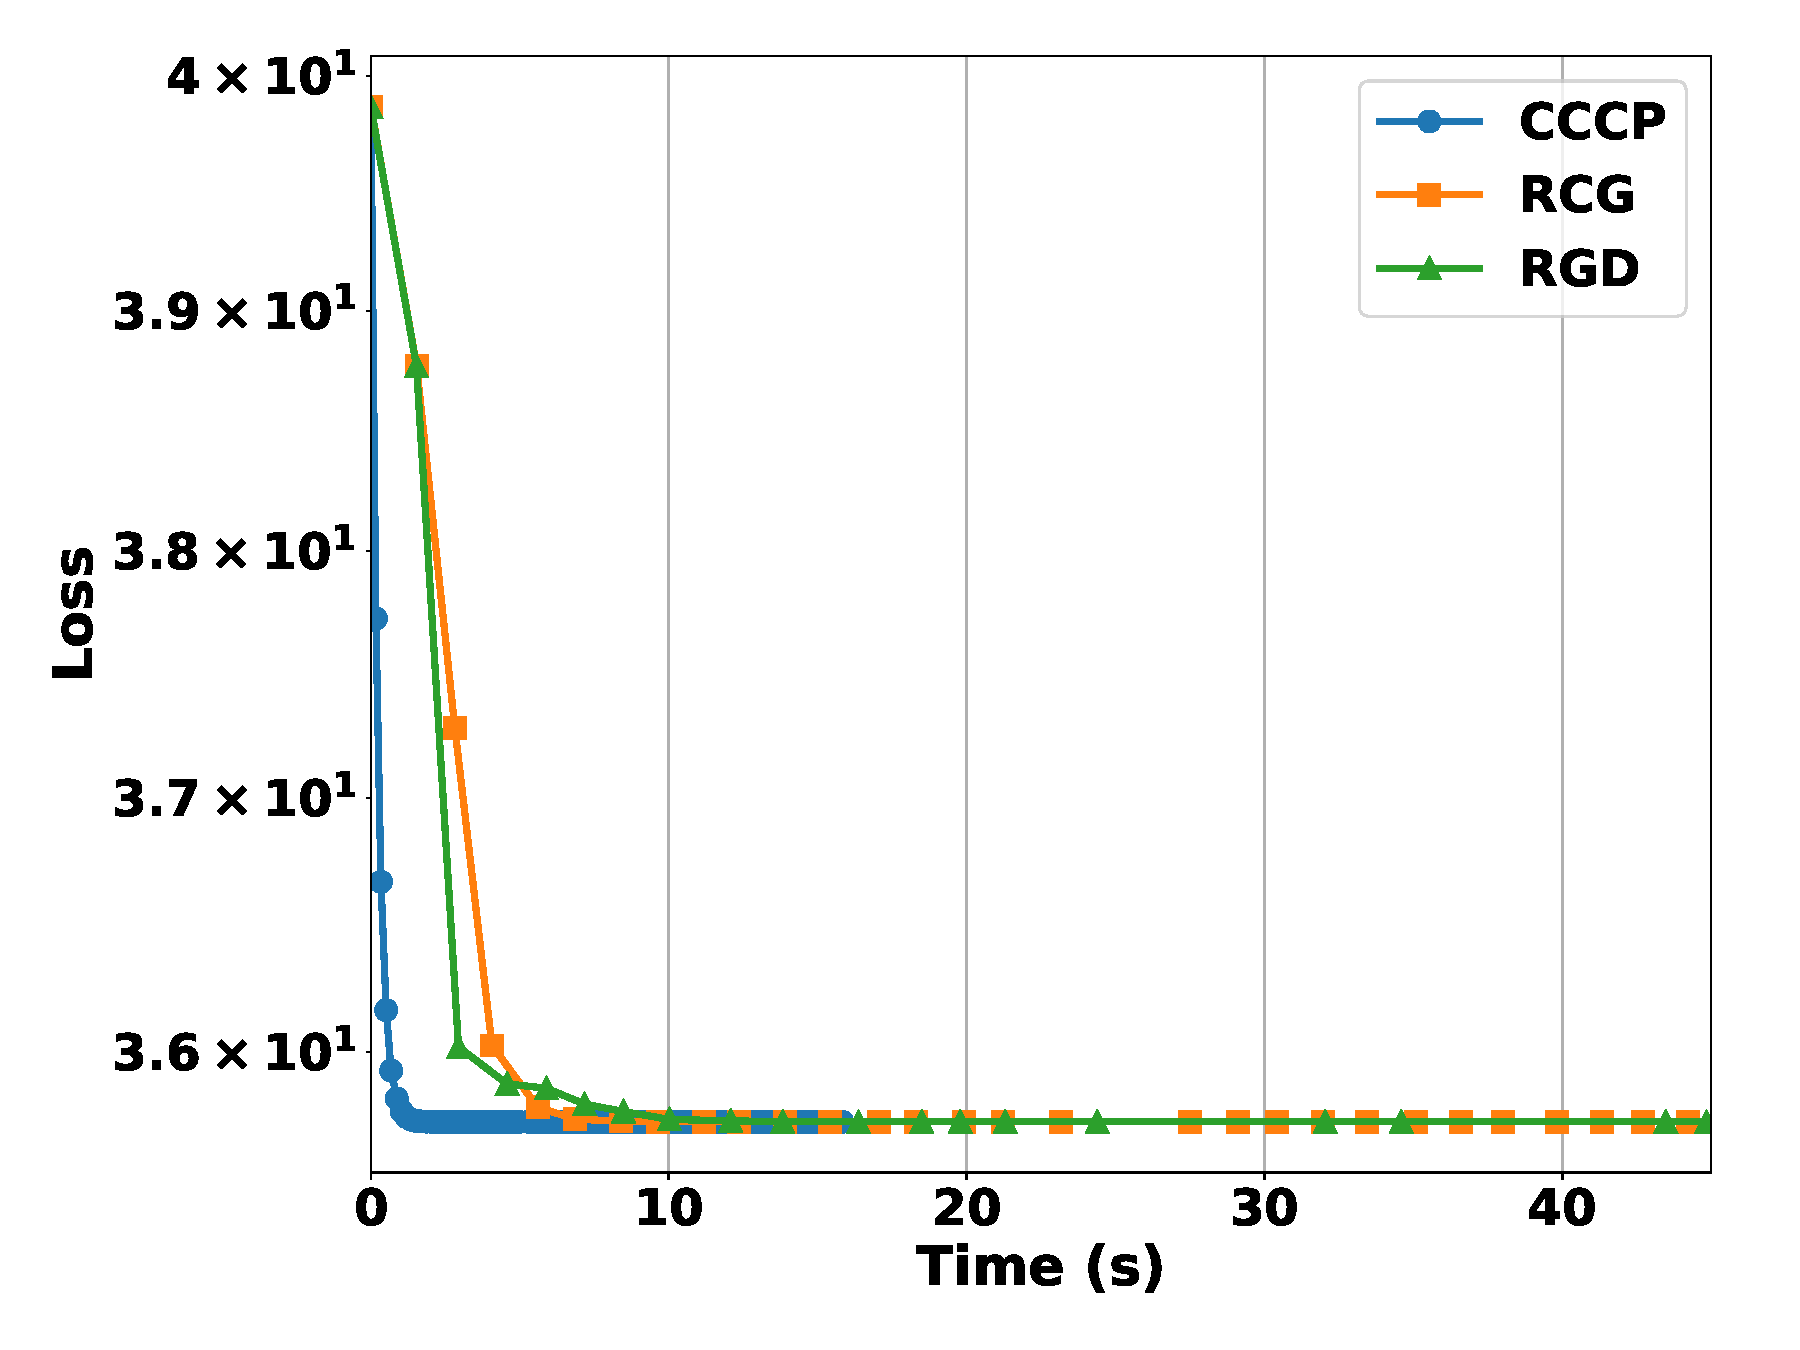
\includegraphics[height=5cm]{figuresV2/karcher_mean/loss_time_500_100_medium.pdf}
%         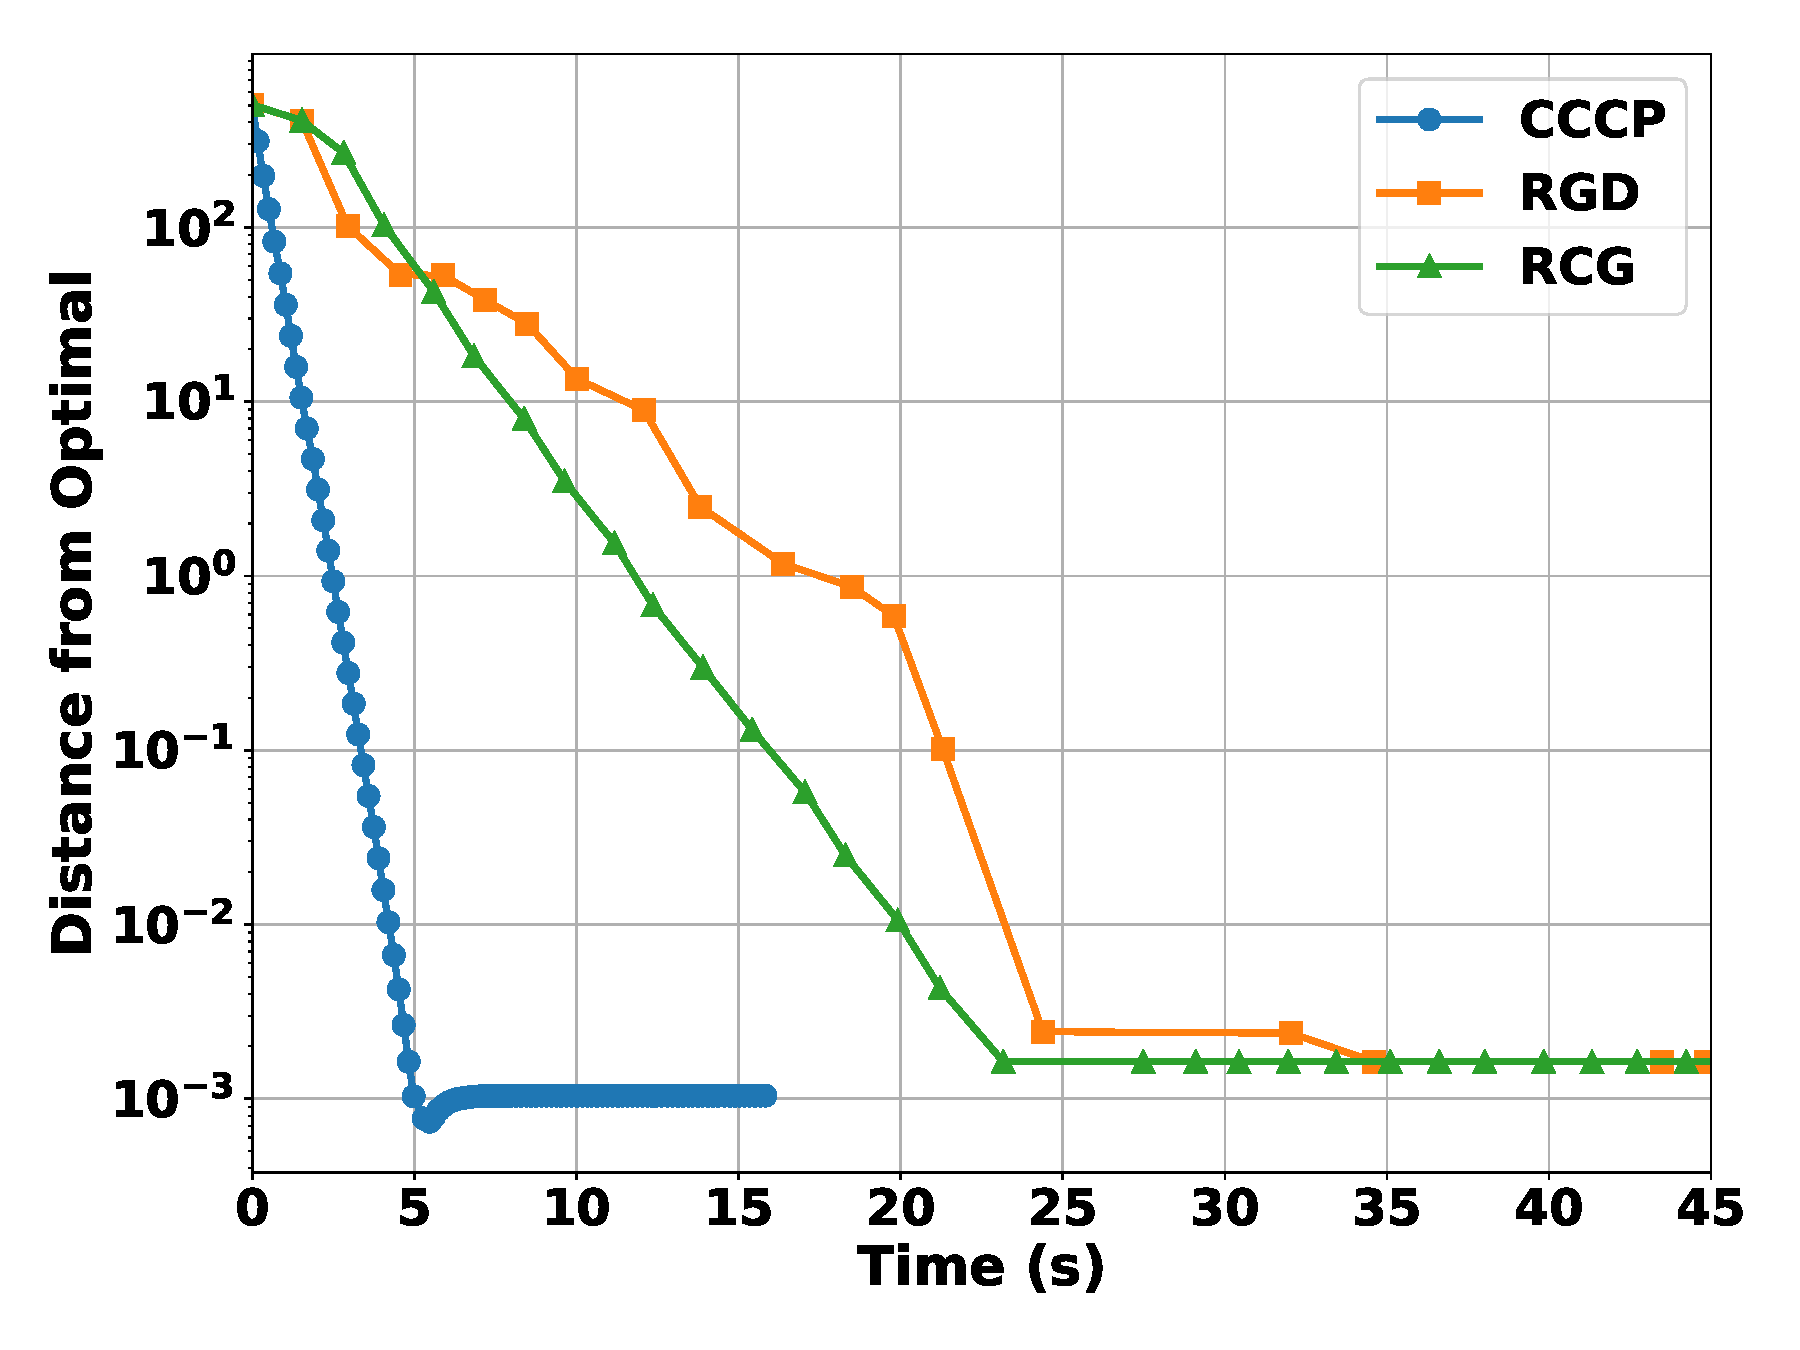
\includegraphics[height=5cm]{figuresV2/karcher_mean/distance_time_500_100_medium.pdf}
%     \caption{\textbf{Karcher Mean.} $m=500$ and $d=100$. We observe that the gap between the runtime performance between CCCP and the benchmarks widens as we take the number of samples $m$ to be larger.}
%     \label{fig:karche_mean_500_100}
% \end{figure}

% \begin{figure}[ht]
%     \centering
%      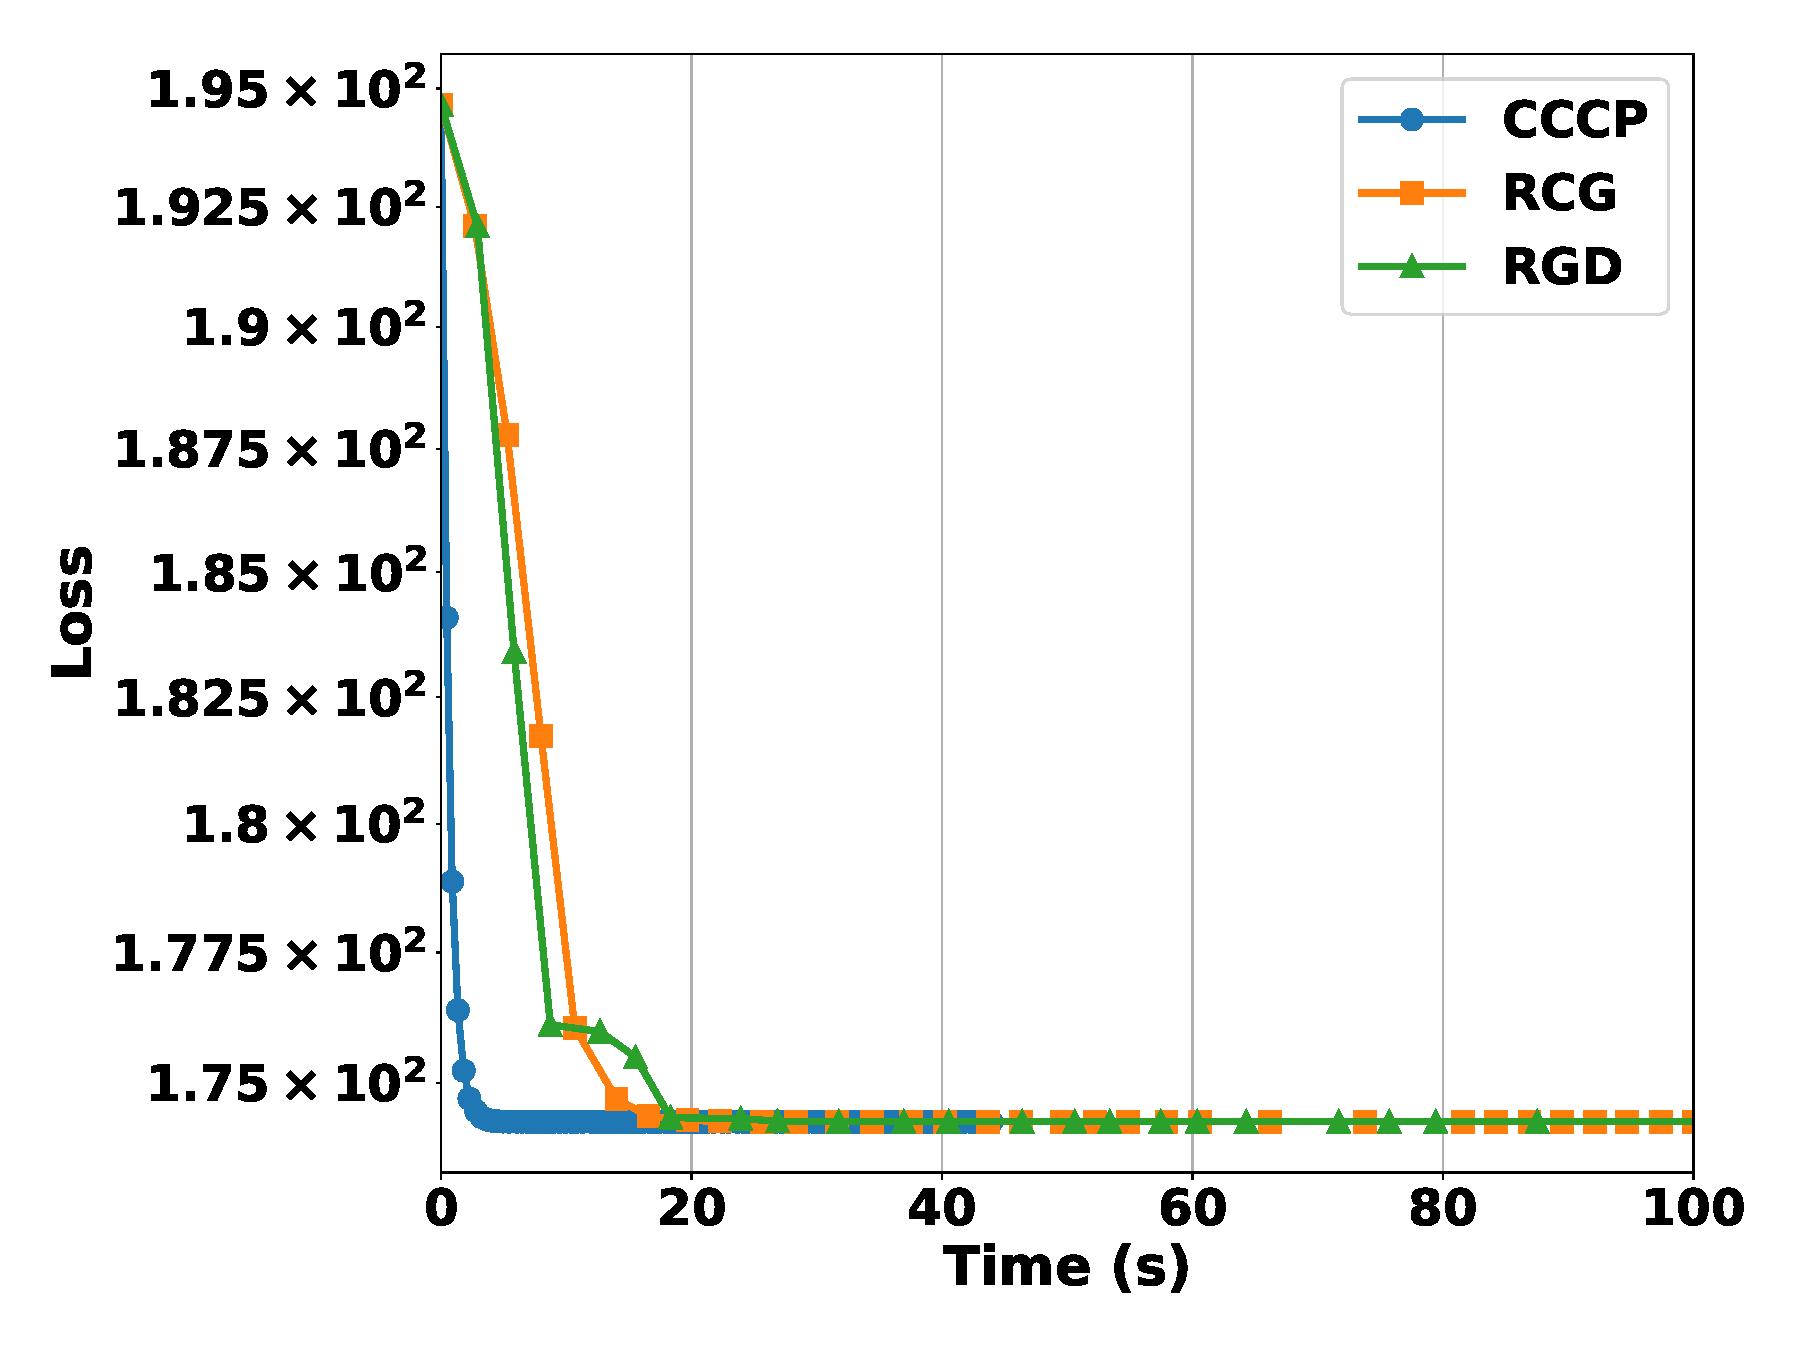
\includegraphics[height=5cm]{figuresV2/karcher_mean/loss_time_100_500_medium.pdf}
%         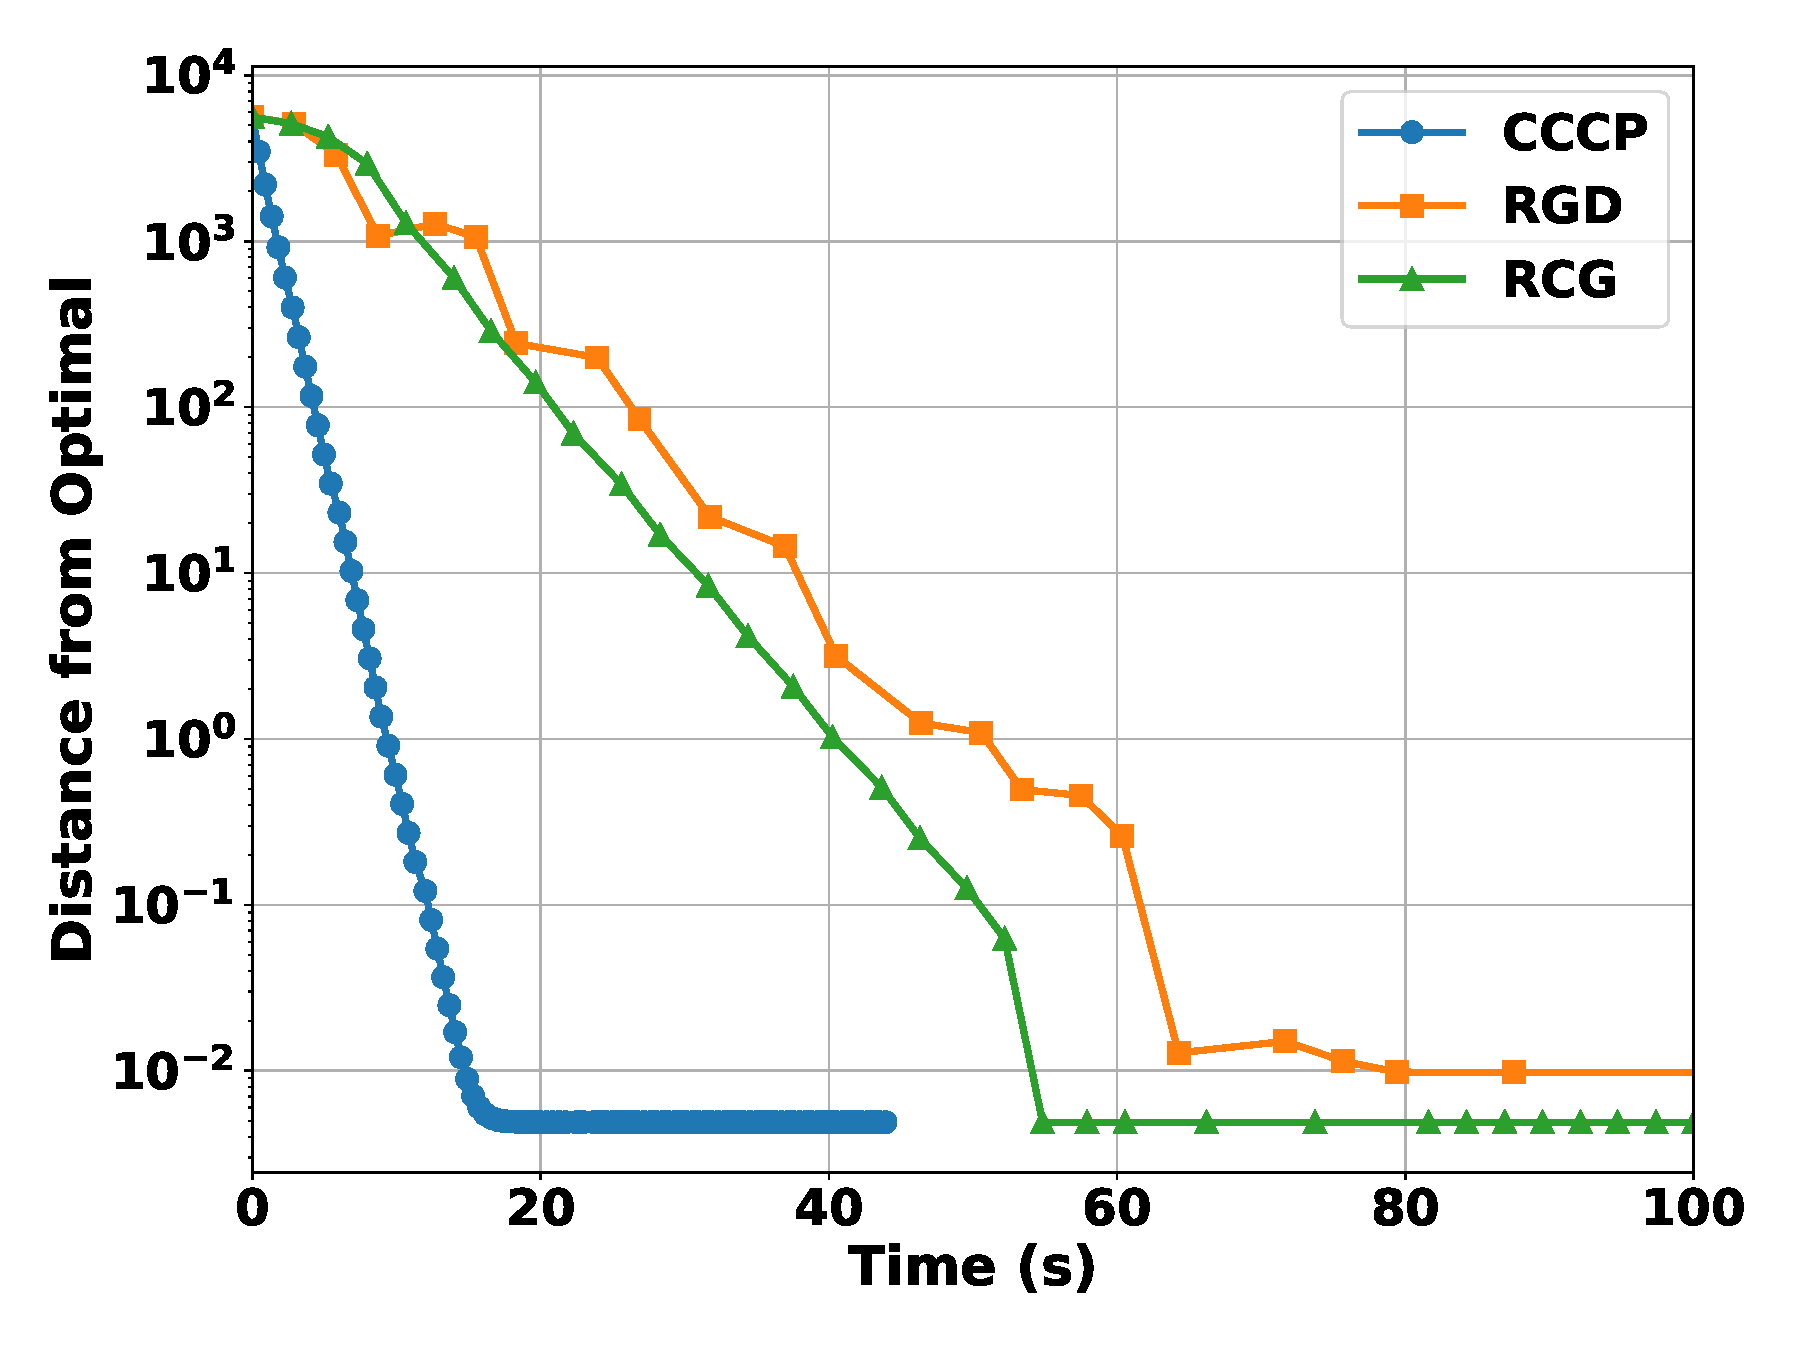
\includegraphics[height=5cm]{figuresV2/karcher_mean/distance_time_100_500_medium.pdf}
%     \caption{\textbf{Karcher Mean} $m=100$ and $d=500$. We observe that the gap between the runtime performance between CCCP and the benchmarks widens as we take the dimension $d$ to be larger.}
%     \label{fig:karche_mean_100_500}
% \end{figure}


% \begin{figure}[htbp]
%   \centering
%   \begin{minipage}[b]{0.45\textwidth}
%     \centering
%     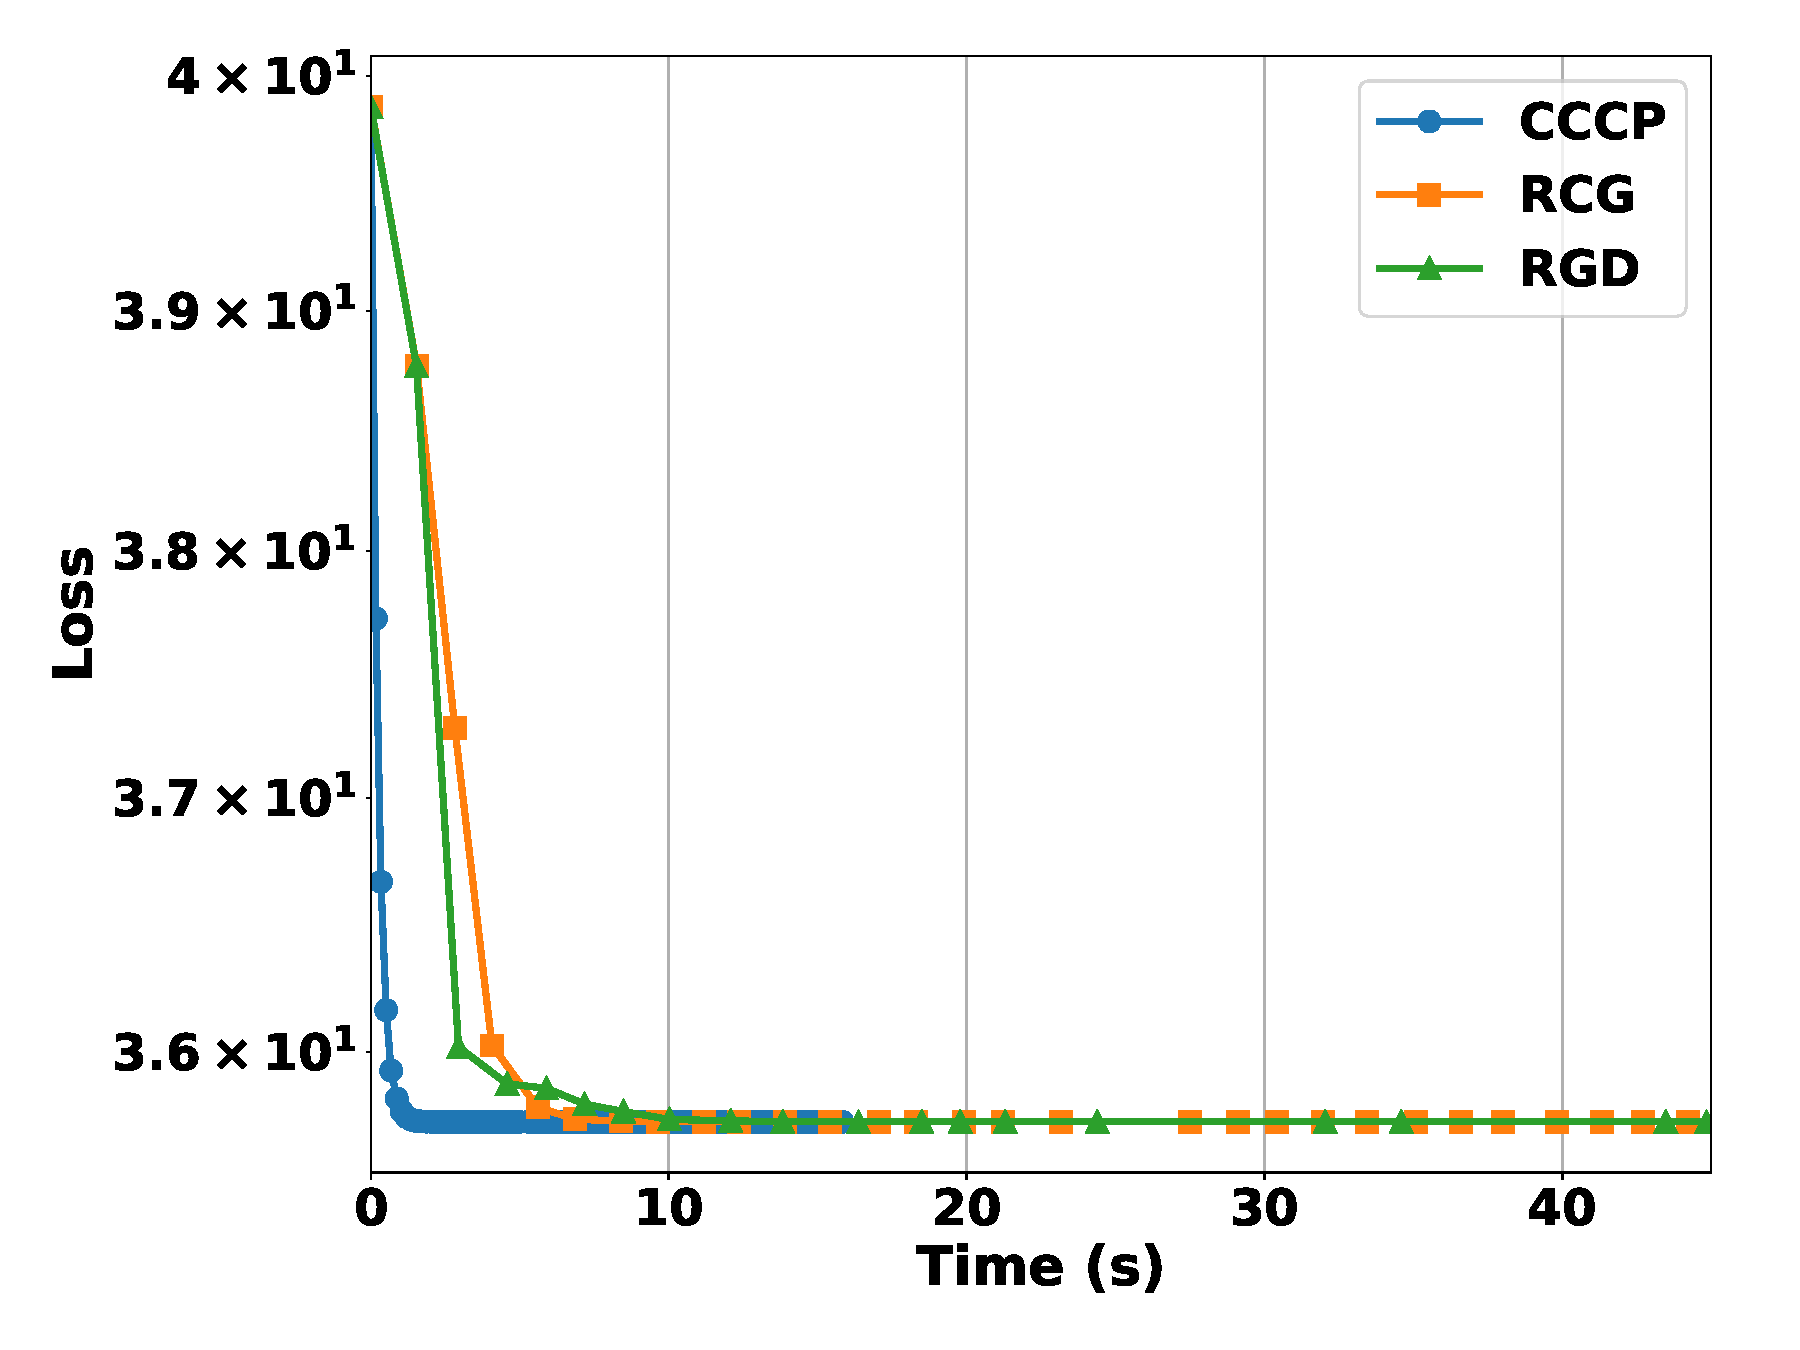
\includegraphics[width=\textwidth]{figuresV2/karcher_mean/loss_time_500_100_medium.pdf}
%   \end{minipage}
%   \hfill
%   \begin{minipage}[b]{0.45\textwidth}
%     \centering
%     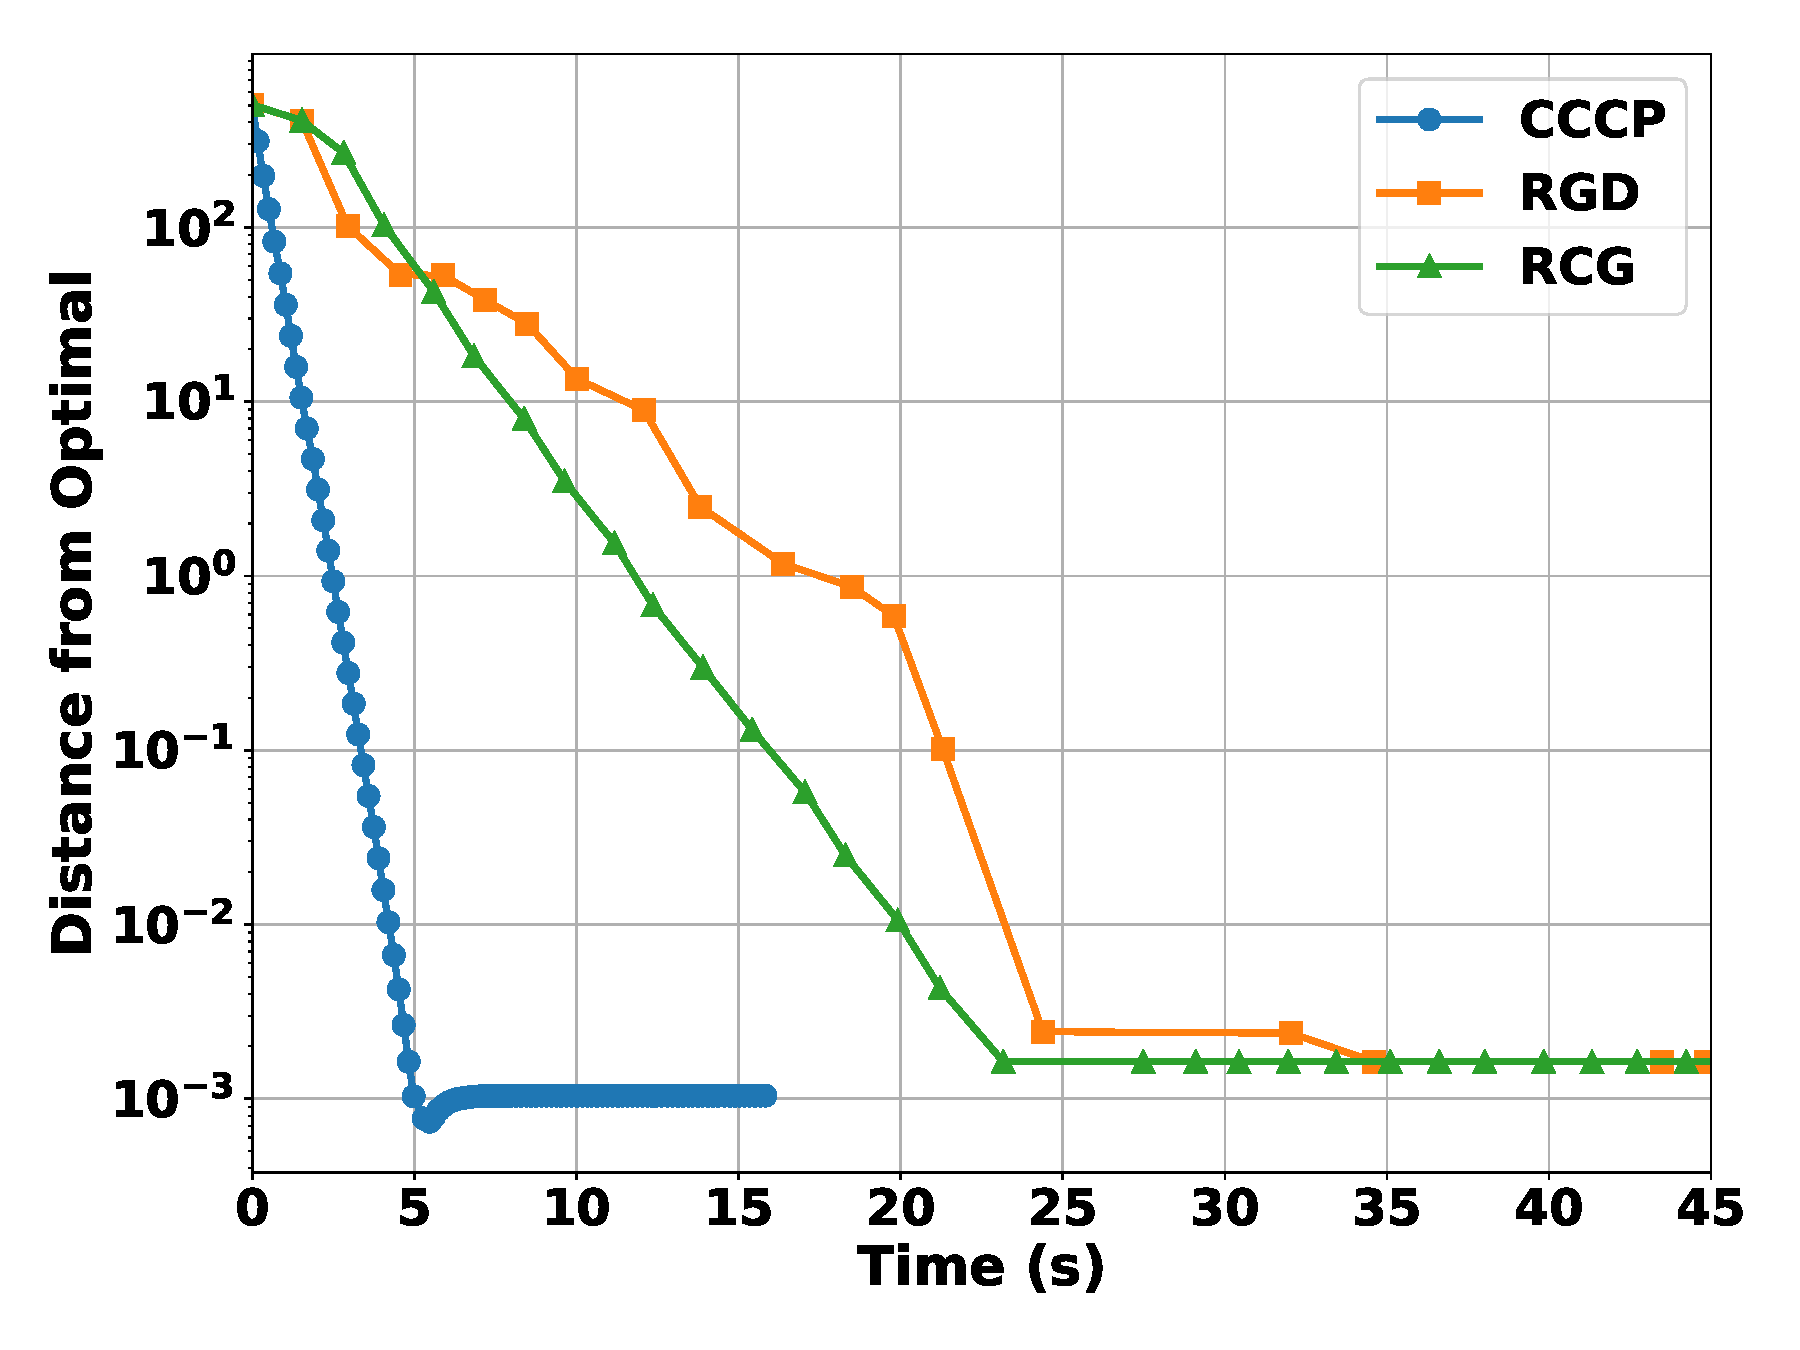
\includegraphics[width=\textwidth]{figuresV2/karcher_mean/distance_time_500_100_medium.pdf}
%   \end{minipage}
%   \caption{\textbf{Karcher Mean.} $m=500$ and $d=100$. We observe that the gap between the runtime performance between CCCP and the benchmarks widens as we take the number of samples $m$ to be larger.}
%   \label{fig:karche_mean_500_100}
% \end{figure}



%\mw{TODO: Adding discussion on complexity of results.}

% In the \textit{ill-conditioned} setting, we sample \textit{m} number of $d \times d$ matrices $U^{(k)}$ whose entries are i.i.d distributed as $U^{(k)}_{ij} \in \mathcal{U}(0,1)$. We project each $U^{(k)}$ onto the closest rank $\ell$ matrix for some $1 \leq \ell < d$, say $\operatorname{Proj}_\ell(U^{(k)})$. Then we construct $A_k = \operatorname{Proj}_\ell(U^{(k)}) \operatorname{Proj}_\ell(U^{(k)})^\top + \delta I_d$ for $k \in [m]$ for some small $\delta > 0$. 




% \begin{figure}
%     \centering
%     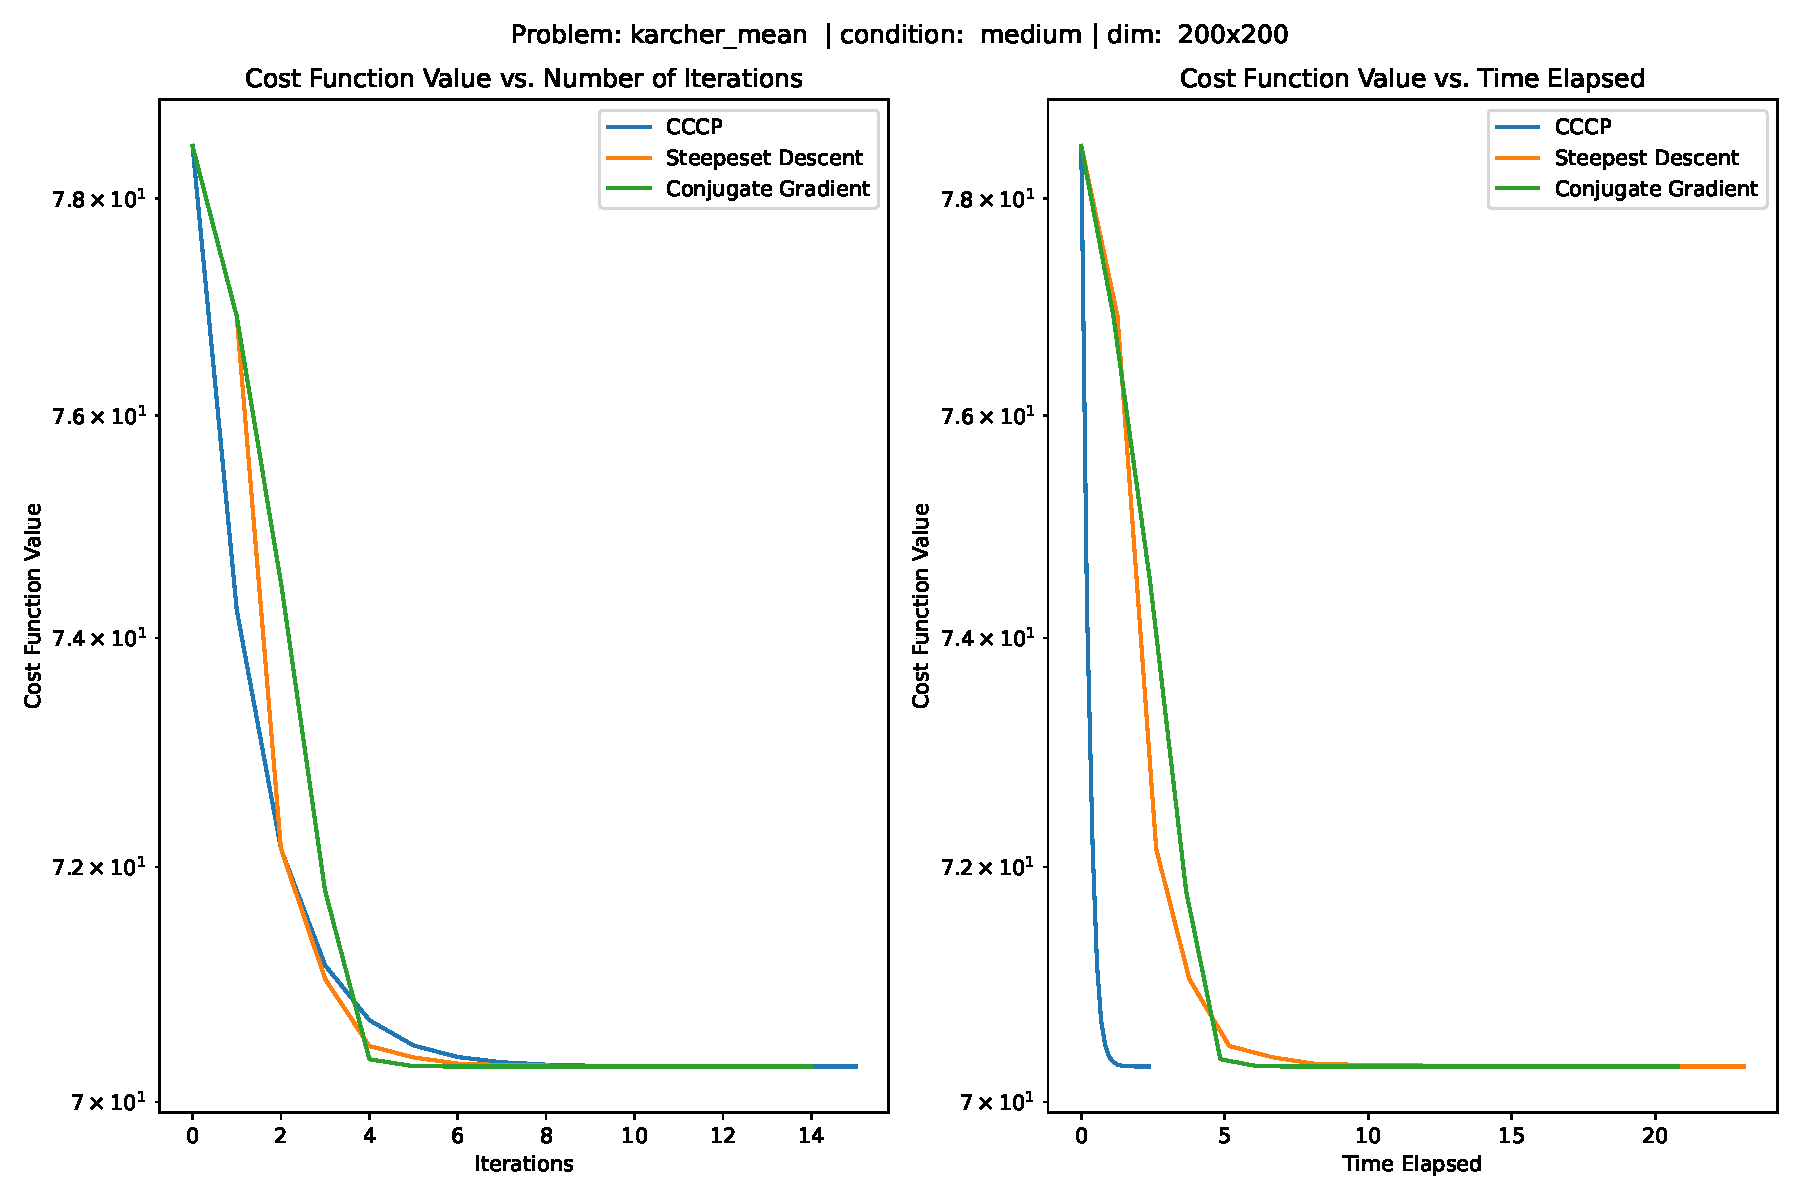
\includegraphics[width=15cm]{figures/karcher_mean_medium_SDRGD_curves.pdf}
%     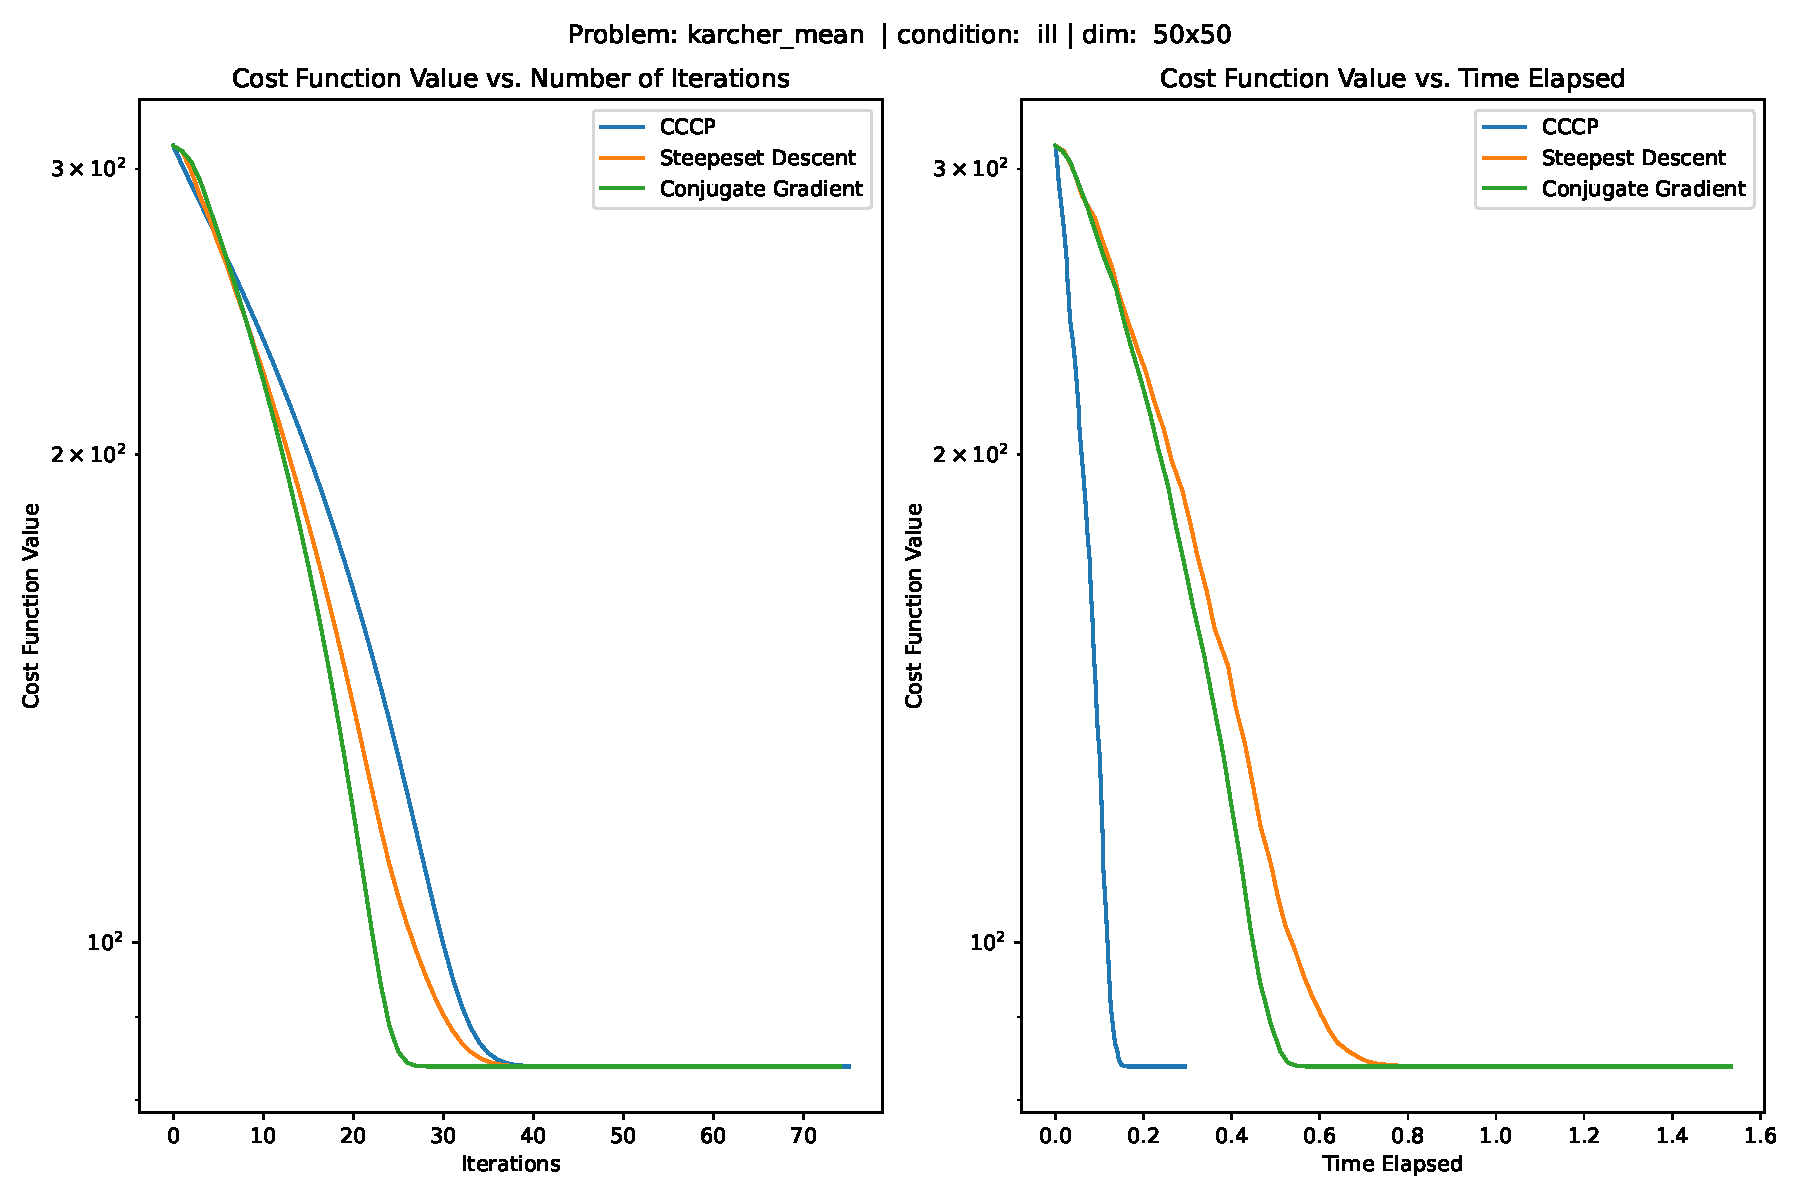
\includegraphics[width=15cm]{figures/karcher_mean_ill_SDRGD_curves.pdf}
%     \caption{\mw{make consistent with landscape format used in the other plots} For each experiment we simulated $m=200$ matrices each with dimension $d=200$. We observe comparable iteration complexity, but the fixed-point algorithm~\eqref{eq:karcher_fp} is superior in runtime performance. In the ill-conditioned case, we project onto the closest rank $50$ matrix $P_i$ and construct our PSD data as $A_i = P_i P_i^\top + 1e-7 I_d$. }
%     \label{fig:karcher_mean}
% \end{figure}




\newpage
\subsection{Optimistic Gaussian Likelihood}\label{section:gaussian_aux_mle}
In this section, we test the performance of CCCP on the problem of computing the optimistic likelihood, introduced in sec.~\ref{sec:GaussianMLE_intro}:

\begin{equation}\label{exp:sdiv_ball_MLE_Problem}
\begin{aligned}
    &\argmin_{\Sigma \in \pd} \left\{ \hat{\phi}(\Sigma) \defas \tr\left(S \Sigma^{-1}\right) + \log \det \Sigma  + \beta \delta_S^2\left(\Sigma, \hat{\Sigma}\right) \right\}. 
\end{aligned}    
\end{equation}


\paragraph{Data Generation}
We follow an experimental setup similar to that of~\cite{Nguyen2019CalculatingOL}. In particular, we generate the true covariance $\Sigma$ and its estimate $\hat{\Sigma} \in \pd$ as follows. First we draw a Gaussian random matrix $A$ with i.i.d. entries $A_{ij} \sim \mathcal{N}(0,1)$. Then we symmetrize and ensure it is positive definite via $\Sigma = \frac{1}{2}\left(A + A^\top\right) + \delta I$. To construct $\hat{\Sigma}$ we conduct the eigenvalue decomposition $\Sigma = Q \Lambda Q^\top$ and replace the eigenvalues in $\Lambda$ with a random diagonal matrix $\hat{D}$ whose diagonal elements are sampled independently and uniformly from $\{1, 2, \ldots, 50\}.$

Our experiments in Figure~\ref{fig:Gaussian_aux_mle_30}
illustrates the output of Algorithm~\ref{alg:CCCP_on_MLE} and its distance from the true covariance $\Sigma$. The trend of the curves matches the intuition that increasing $\beta > 0$ and therefore increasing the confidence in $\hat{\Sigma}$ results in a solution closer to $\hat{\Sigma}$. We also note that higher regularization $\beta > 0$ results in faster convergence as exhibited in Figure~\ref{fig:Gaussian_aux_mle_30}. Moreover, Table~\ref {table:gaussian_aux_norm_master} illustrates the interpolation behaviour of $\hat{\Sigma}_\beta$ between $S$ and $\hat{\Sigma}$ as a function of $\beta$.


\begin{figure}
    \centering
    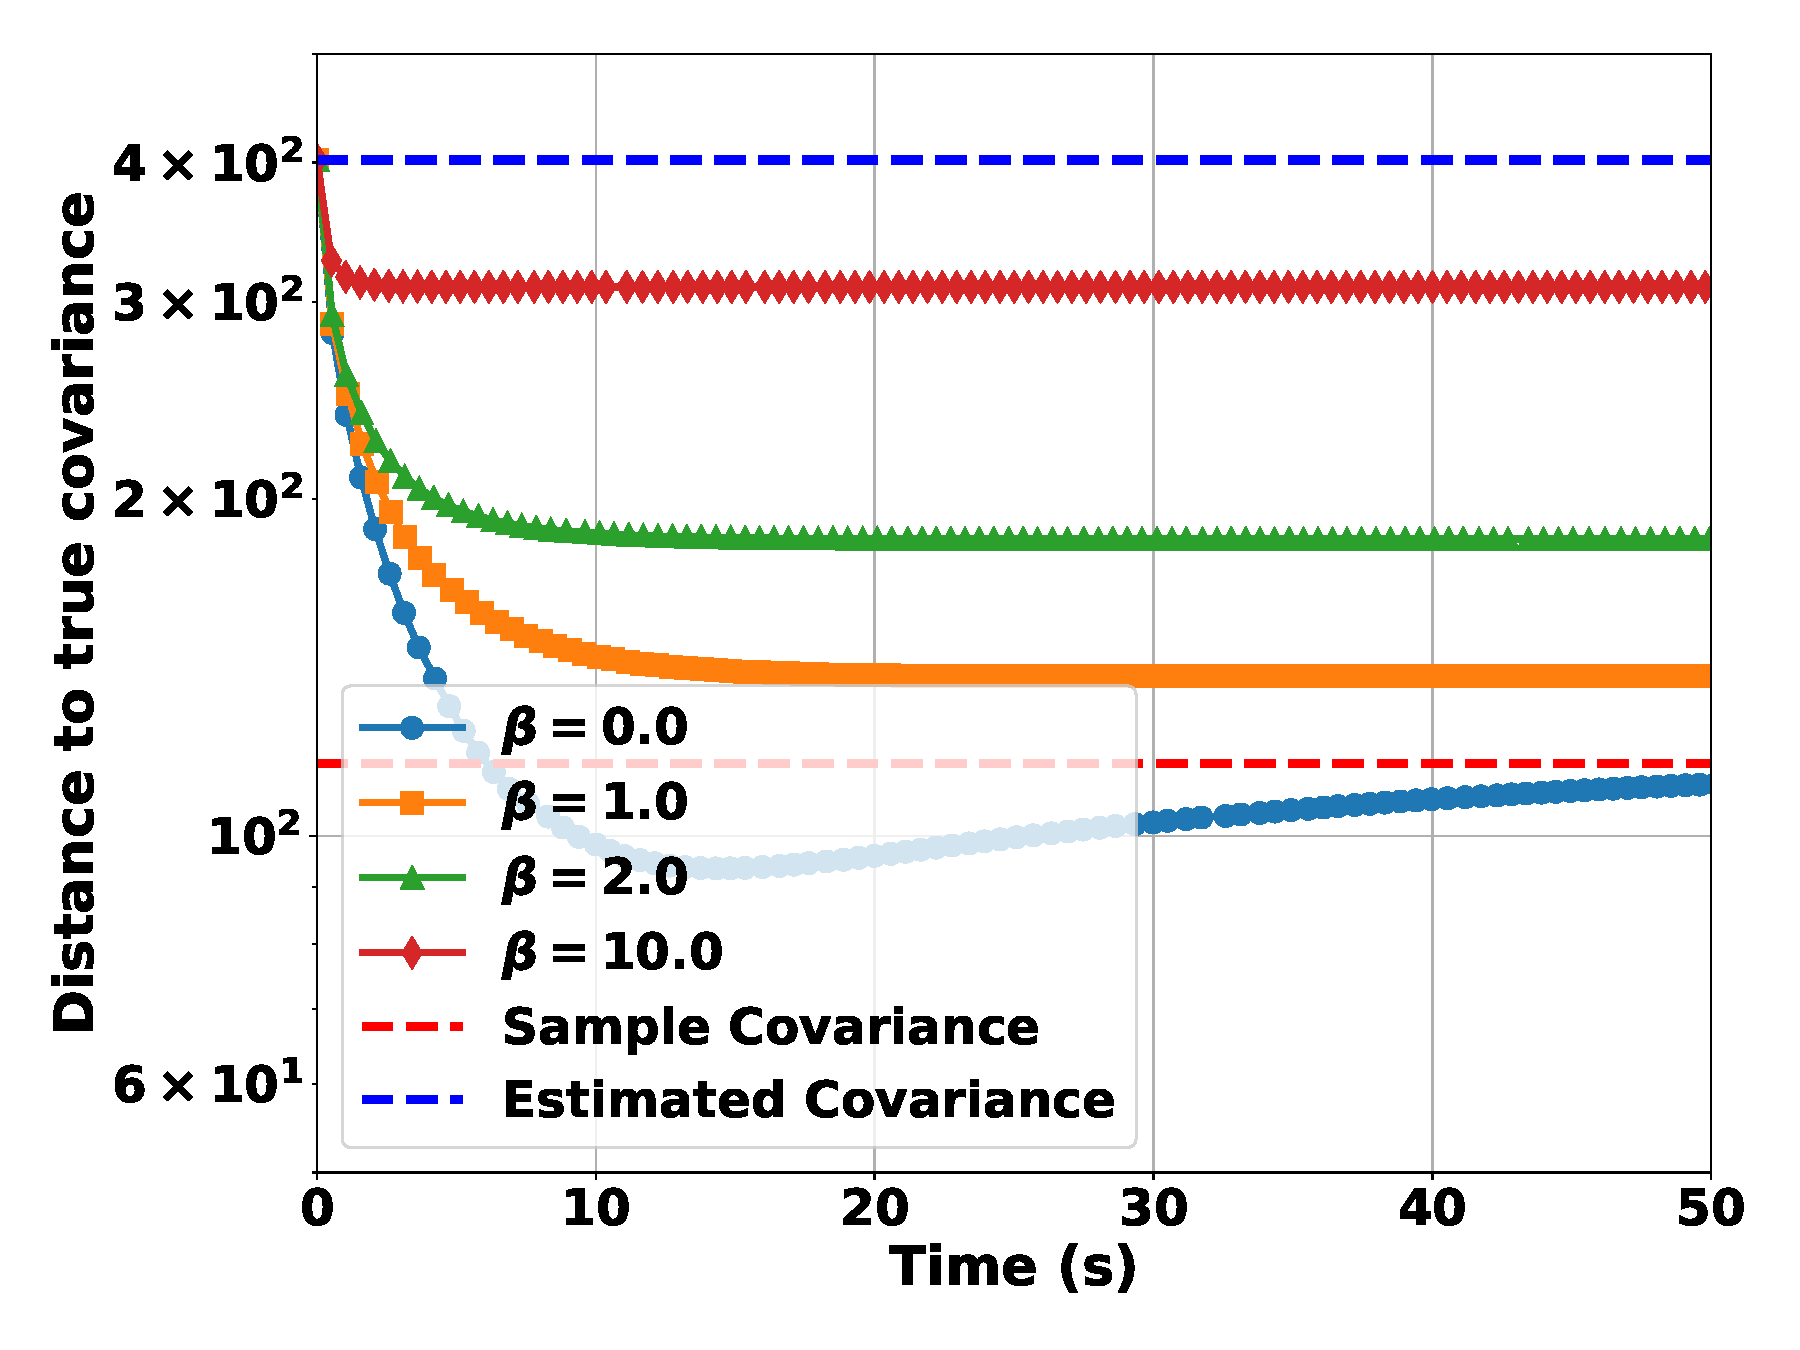
\includegraphics[width=0.43\linewidth]{figuresV2/Gaussian_MLE/cccp_gaussianMLE_30.pdf}
    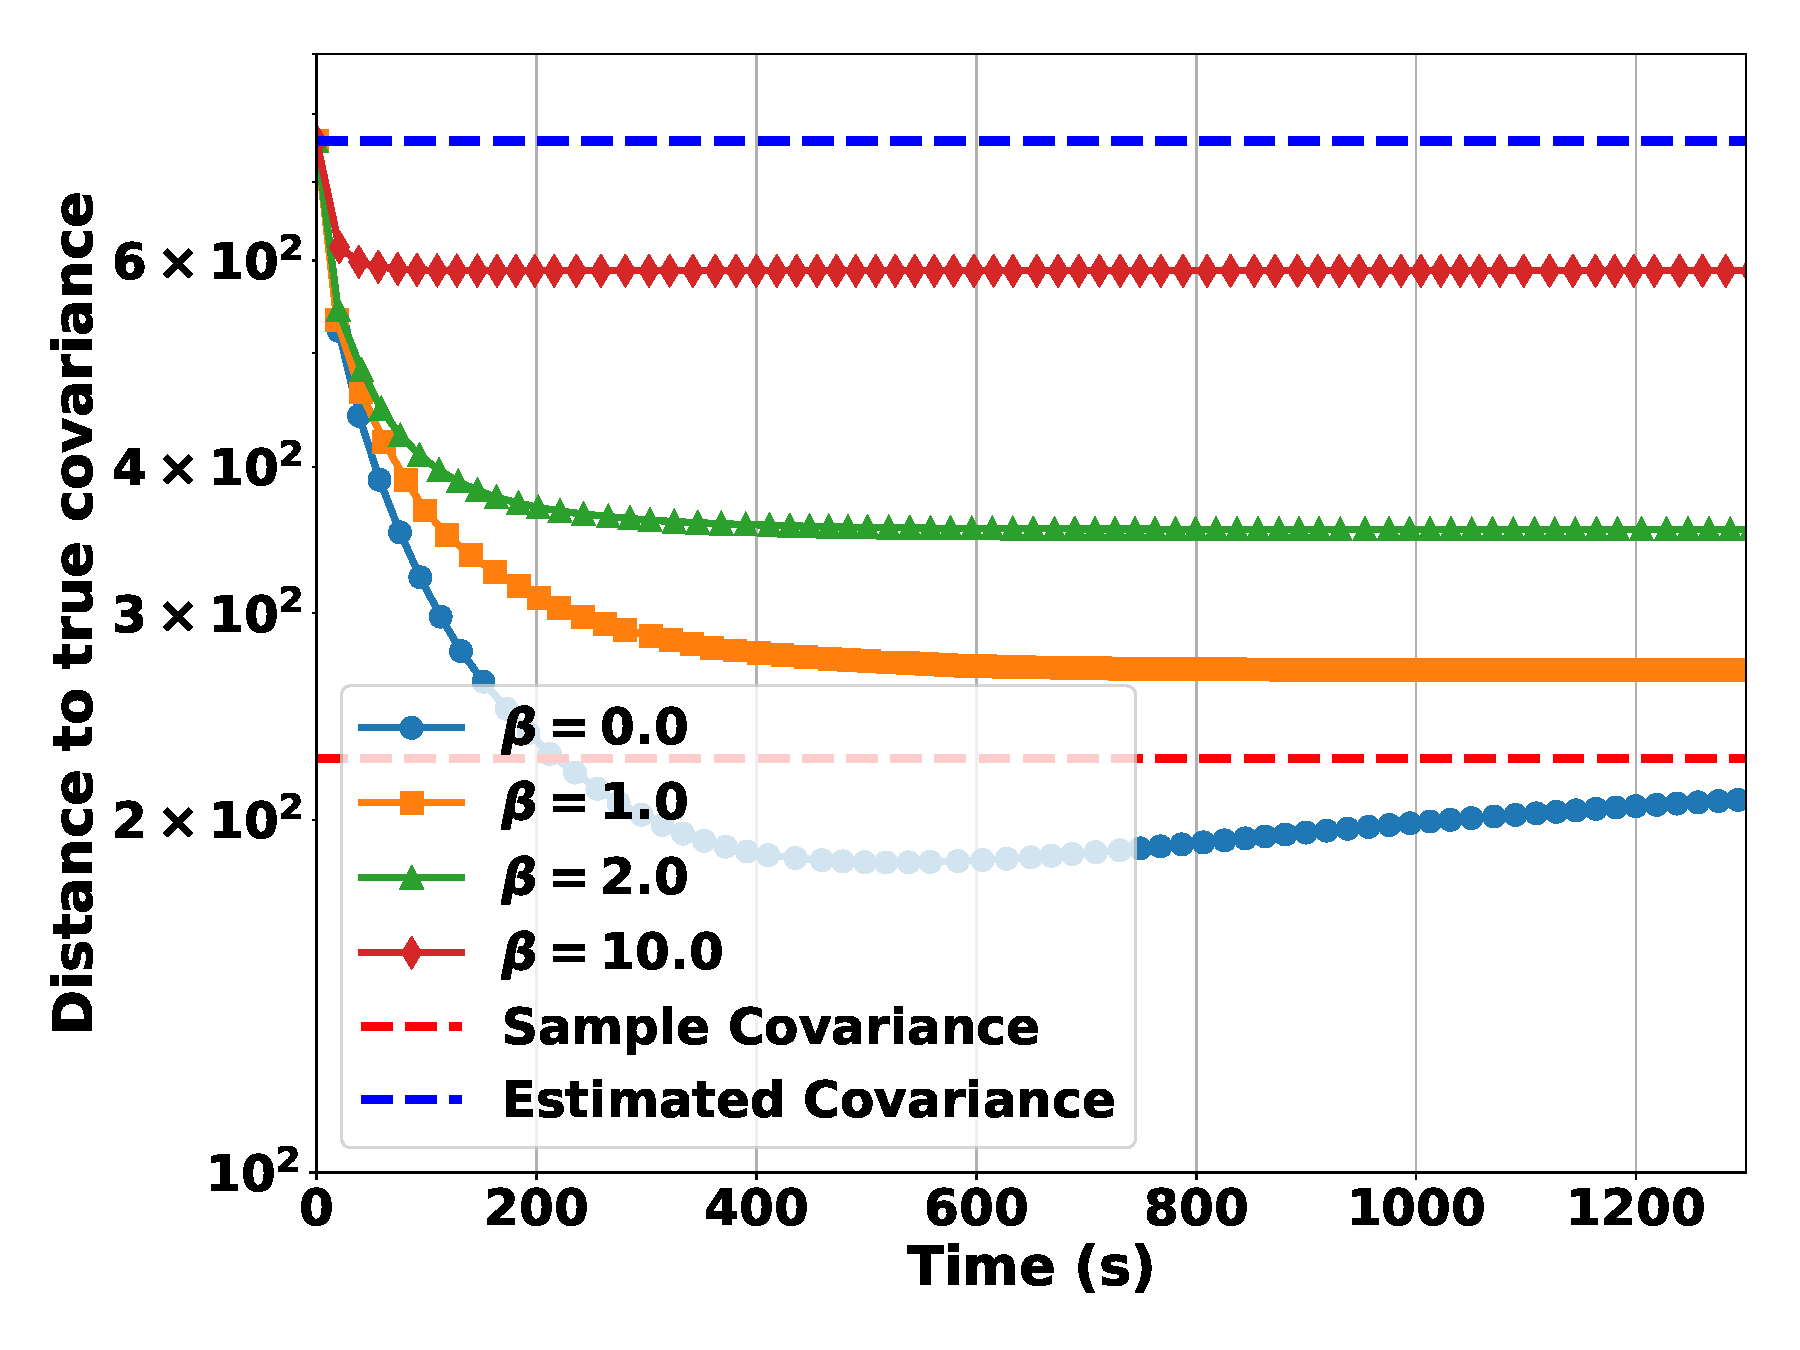
\includegraphics[width=0.43 \linewidth]{figuresV2/Gaussian_MLE/cccp_gaussianMLE_100.pdf}
    \caption{\textbf{Algorithm~\ref{alg:CCCP_on_MLE} on Gaussian Optimistic Likelihood.} We sampled $n=100$ independent Gaussian vectors of dimension $d=30$ for the left plot. Meanwhile, the right plot was generated with $n=1500$ and $d=100$. We initialized our iterate at our estimate $\hat{\Sigma}$.
    As we increase $\beta$, Algorithm~\ref{alg:CCCP_on_MLE} converges to a solution $\hat{\Sigma}_\beta$ closer to $\hat{\Sigma}$. At $\beta = 0$, the algorithm converges to the sample covariance, i.e., $\hat{\Sigma}_\beta = S$. Refer to table~\ref{table:gaussian_aux_norm_master} for the distances between $\|\hat{\Sigma}_\beta  - \Sigma^*\|_F$ and $\|\hat{\Sigma}_\beta - \hat{\Sigma}\|_F$ for varying $\beta$.}
    \label{fig:Gaussian_aux_mle_30}
\end{figure}




% \begin{table}[h!]
% \centering
% \begin{tabular}{|c|c|c|}
% \hline
% $\beta$ & $\|\hat{\Sigma}_\beta - S\|_F$ & $\|\hat{\Sigma}_\beta - \hat{\Sigma}\|_F$ \\ \hline
% 0  & 0.149   & 412.009 \\ \hline
% 1  & 116.545 & 296.022 \\ \hline
% 2  & 178.140 & 234.583 \\ \hline
% 10 & 316.485 & 96.094  \\ \hline
% \end{tabular}
% \begin{tabular}{|c|c|c|}
% \hline
% $\beta$ & $\|\hat{\Sigma}_\beta - S\|_F$ & $\|\hat{\Sigma}_\beta - \hat{\Sigma}\|_F$ \\ \hline
% 0  & 21.741  & 780.233 \\ \hline
% 1  & 231.662 & 566.262 \\ \hline
% 2  & 351.602 & 446.663 \\ \hline
% 10 & 617.255 & 180.798 \\ \hline
% \end{tabular}
% \caption{$\hat{\Sigma}_\beta$ denotes the output of Algorithm~\ref{alg:CCCP_on_MLE} with different $\beta$ values. The left table corresponds to the case $n=100$ and $d =30$. The right table corresponds to $n=1500$ and $d=100$.}
% \label{table:gaussian_aux_norm_master}
% \end{table}

\begin{table}[htbp]
  \centering
  \begin{minipage}{0.45\textwidth}
    \centering
    \begin{tabular}{|c|c|c|}
    \hline
    $\beta$ & $\|\hat{\Sigma}_\beta - S\|_F$ & $\|\hat{\Sigma}_\beta - \hat{\Sigma}\|_F$ \\ \hline
    0  & 0.149   & 412.009 \\ \hline
    1  & 116.545 & 296.022 \\ \hline
    2  & 178.140 & 234.583 \\ \hline
    10 & 316.485 & 96.094  \\ \hline
    \end{tabular}
  \end{minipage}
  \begin{minipage}{0.45\textwidth}
    \centering
    \begin{tabular}{|c|c|c|}
    \hline
    $\beta$ & $\|\hat{\Sigma}_\beta - S\|_F$ & $\|\hat{\Sigma}_\beta - \hat{\Sigma}\|_F$ \\ \hline
    0  & 21.741  & 780.233 \\ \hline
    1  & 231.662 & 566.262 \\ \hline
    2  & 351.602 & 446.663 \\ \hline
    10 & 617.255 & 180.798 \\ \hline
    \end{tabular}
  \end{minipage}
  \caption{$\hat{\Sigma}_\beta$ denotes the output of Algorithm~\ref{alg:CCCP_on_MLE} with different $\beta$ values. The left table corresponds to the case $n=100$ and $d =30$. The right table corresponds to $n=1500$ and $d=100$.}
  \label{table:gaussian_aux_norm_master}
\end{table}


\subsection{Optimistic Multivariate T-Likelihood}
% In this section, we illustrate how one can apply Algorithm~\ref{alg:CCCP_on_Kotz} to a specific elliptically contoured distribution. In this case, we focus on the $d$-dimensional mean zero multivariate $t$-distribution with $\nu >0$ degrees of freedom and parameterized by the scatter matrix $\Sigma \in \pd$. We denote this distribution as $\operatorname{MVT}(\Sigma; \nu)$. It has the density 
% \[
% f_X(x;\nu) = \frac{\Gamma[(\nu+d) / 2]}{\Gamma(\nu / 2) \nu^{d / 2} \pi^{d / 2}|{\Sigma}|^{1 / 2}}\left[1+\frac{1}{\nu}({x}-{\mu})^T {\Sigma}^{-1}({x}-{\mu})\right]^{-(\nu+d) / 2}.
% \]
% Its negative log-likelihood is proportional to $T_\nu(\Sigma)$ given by 
% \[
% T_\nu(\Sigma) = \frac{n}{2}\log \det \Sigma + \frac{\nu + d}{2}\sum_{i=1}^n \log \left( 1 + \frac{1}{\nu}x_i^\top \Sigma^{-1}x_i\right) + \gamma \log \det \left(\frac{\Sigma + \hat{\Sigma}}{2}\right) - \frac{\gamma }{2}\log \det \left(\Sigma \hat{\Sigma}\right)
% \]

% The multivariate $t$-distribution is a generalization of several well-known distributions. For example, we recover the Student's $t$ distribution  by taking $d=1$ and $\Sigma = 1$. Taking $\nu \to +\infty$ recovers the multivariate normal density with mean 0 and covariance $\Sigma$. Taking $\nu = 1$ recovers the $d$-variate Cauchy distribution and taking $\frac{\nu + d}{2}$ to be an integer recovers the $d$-variate Pearson type VII distribution \cite{Kotz2004}. 


% Due to its ability to capture tail events (data involving errors with heavier than Gaussian tails), the multivariate t distribution is often used for robust statistical modelling especially when the assumptions of normality is violated \cite{Lange1989} \cite{Nadarajah2005}. 


% For additional information $\hat{\Sigma}\in \pd$ the corresponding optimistic likelihood problem is 
% \begin{equation}\label{eq:multivariate_t_aux}
%     \Sigma^* = \argmin_{\Sigma \in \pd} \left\{ \hat{\phi}(\Sigma) \defas  T_\nu(\Sigma) + \gamma \delta_S^2 \left(\Sigma, \hat{\Sigma}\right) \right\}
% \end{equation}
% where $\gamma > 0$ is a hyperparameter that denotes our confidence in $\hat{\Sigma}.$ 

% \begin{algorithm}[H]\label{alg:aux_multivar_T}
% \SetAlgoLined
% \textbf{Input:} $\Sigma_0, \hat{\Sigma} \in \pd$, $K, L \in \nat$, $\gamma, \nu > 0$ and $\{\eta_\ell\} \subseteq \real_{++}$\\
%  \For{$k = 0, \ldots, K-1$}{
%  Precompute $\gamma \left(\Sigma_k + \hat{\Sigma}_k\right)^{-1} + \frac{n}{2}\Sigma_k^{-1}$ \\
%  \For{$\ell = 0, \ldots, L-1$}{
%     $\Sigma_{\ell+1} \leftarrow  \Sigma_\ell - \eta_\ell \left(- \frac{\nu + d}{2} \Sigma_\ell^{-1} \left(\sum_{i=1}^n \frac{x_i x_i^\top}{\nu + x_i^\top \Sigma_\ell^{-1} x_i} \right)\Sigma_\ell^{-1}  - \frac{\gamma}{2}\Sigma_\ell^{-1} +  \gamma \left(\Sigma_k + \hat{\Sigma}_k\right)^{-1} + \frac{n}{2}\Sigma^{-1}_k\right) $
%     }
% Update $\Sigma_{k+1} \leftarrow \Sigma_{L}$\\
% }
% \textbf{Output:} $\Sigma_K$
% \caption{CCCP on Multivariate T Optimistic Likelihood}
% \end{algorithm}


% In order to solve the optimization problem \eqref{eq:multivariate_t_aux} we appeal to the CCCP algorithm. In particular, to adapt Algorithm~\ref{alg:CCCP_on_Kotz} to our setting, we can group the convex and concave terms of $\hat{\phi}(\Sigma)$ into the functions $f(\Sigma)$ and $g(\Sigma)$, respectively:

% \[
% \begin{aligned}
%     f(\Sigma) = \frac{\nu + d}{2}\sum_{i=1}^n \log \left(1 + \frac{1}{\nu}x_i^\top \Sigma^{-1}x_i\right) - \frac{\gamma}{2}\log \det \left(\Sigma \hat{\Sigma}\right) \\
%     g(\Sigma) = \frac{n}{2}\log \det \Sigma + \gamma \log \det \left( \frac{\Sigma + \hat{\Sigma}}{2} \right)
% \end{aligned}
% \]

% Their gradients are computed as 
% \[
% \begin{aligned}
% &\nabla f(\Sigma) = - \frac{\nu + d}{2} \Sigma^{-1} \left(\sum_{i=1}^n \frac{x_i x_i^\top}{\nu + x_i^\top \Sigma^{-1} x_i} \right)\Sigma^{-1}  - \frac{\gamma}{2}\Sigma^{-1}
% \\&\nabla g(\Sigma) = \gamma \left(\Sigma + \hat{\Sigma}\right)^{-1} + \frac{n}{2}\Sigma^{-1}
% \end{aligned}
% \]

% The convex CCCP surrogate function can be written as $Q(\Sigma, \Sigma_k) = f(\Sigma) + \langle g(\Sigma_k), \Sigma - \Sigma_k \rangle$ for convex $f$ and concave $g$. Thus to solve for $\argmin_{\Sigma \in \pd} Q(\Sigma, \Sigma_k)$ we can apply the gradient descent steps: 
% \[
% \Sigma_{\ell+1} \leftarrow \Sigma_{\ell} - \eta_\ell \left( \nabla f(\Sigma_\ell) + \nabla g\left(\Sigma_k\right)\right)
% \]
% for a sequence of step-sizes $\{\eta_\ell\}$. All in all, we have algorithm~\ref{alg:aux_multivar_T}.
 We perform an experiment similar to that in the previous section for Algorithm~\ref{alg:aux_multivar_T}.
 We generate $d$-dimensional random vectors $x_1, \ldots, x_n \stackrel{\text{iid}}{\sim} \operatorname{MVT}(\Sigma; \nu)$ and observe the output of Algorithm~\ref{alg:aux_multivar_T} for different values of $\gamma$. We observe that incorporating $\hat{\Sigma}$ improves the distance from optimality. However, we observed that this method requires a high number of data points (See Figure~\ref{fig:multivar_t_aux_high_samples}).
%  \begin{wrapfigure}{R}{0.3\linewidth}
%     \centering
%     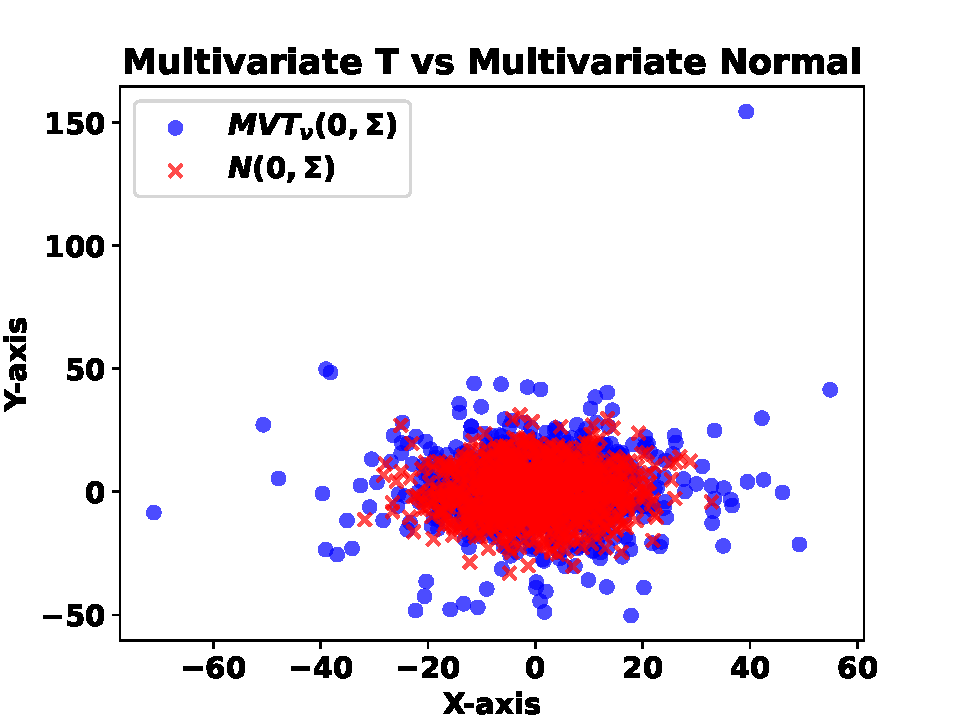
\includegraphics[width=\linewidth]{figuresV2/multivar_t/mvt_vs_normal.pdf}
%     \caption{\textbf{Gaussian vs. Multivariate t Distribution.} Taking $d=2$ and generating $n=1000$ samples from $N(0,\Sigma)$ and $\operatorname{MVT}(\Sigma; \nu=5)$ with $\Sigma$ generated as in Section~\ref{section:gaussian_aux_mle}. The heavier tails of the multivariate t distribution manifests in the outliers relative to the normal distribution.} 
%     \label{fig:enter-label}
% \end{wrapfigure}

\begin{figure}[ht]
    \centering
    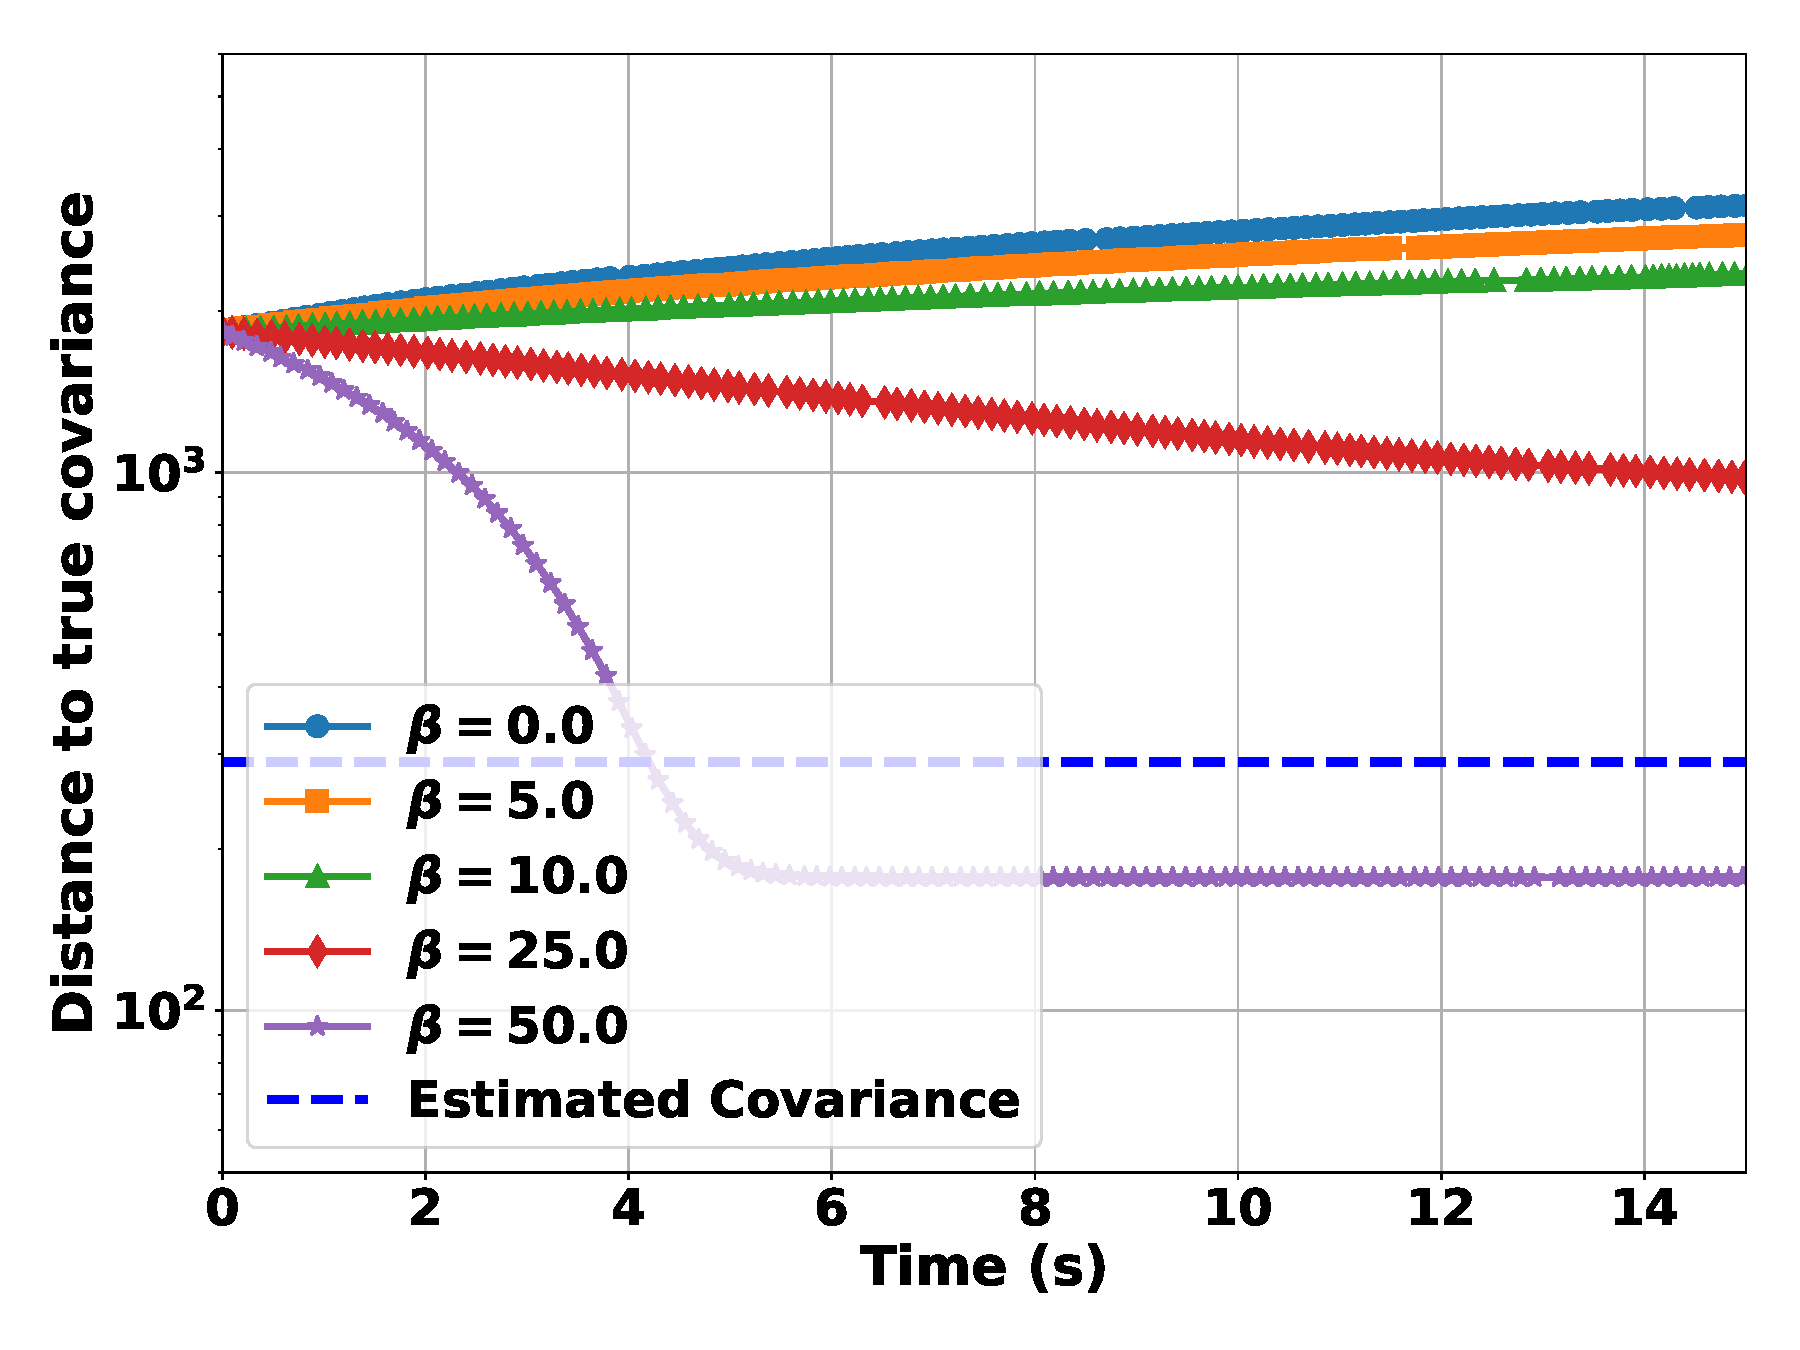
\includegraphics[width=0.43\linewidth]{figuresV2/multivar_t/t_aux_nu5_d15_n1200.pdf}
    \caption{\textbf{Multivariate T-Distribution Optimistic Likelihood.} We sampled $n=1200$ i.i.d. multivariate t vectors of dimension $d=15$. The plot indicates similar behaviour of that to the Gaussian optimistic likelihood problem: higher regularization encourages solution to be nearer $\hat{\Sigma}$ and also exhibits faster convergence.}
    \label{fig:multivar_t_aux_figs}
\end{figure}



\begin{figure}[ht]
    \centering
    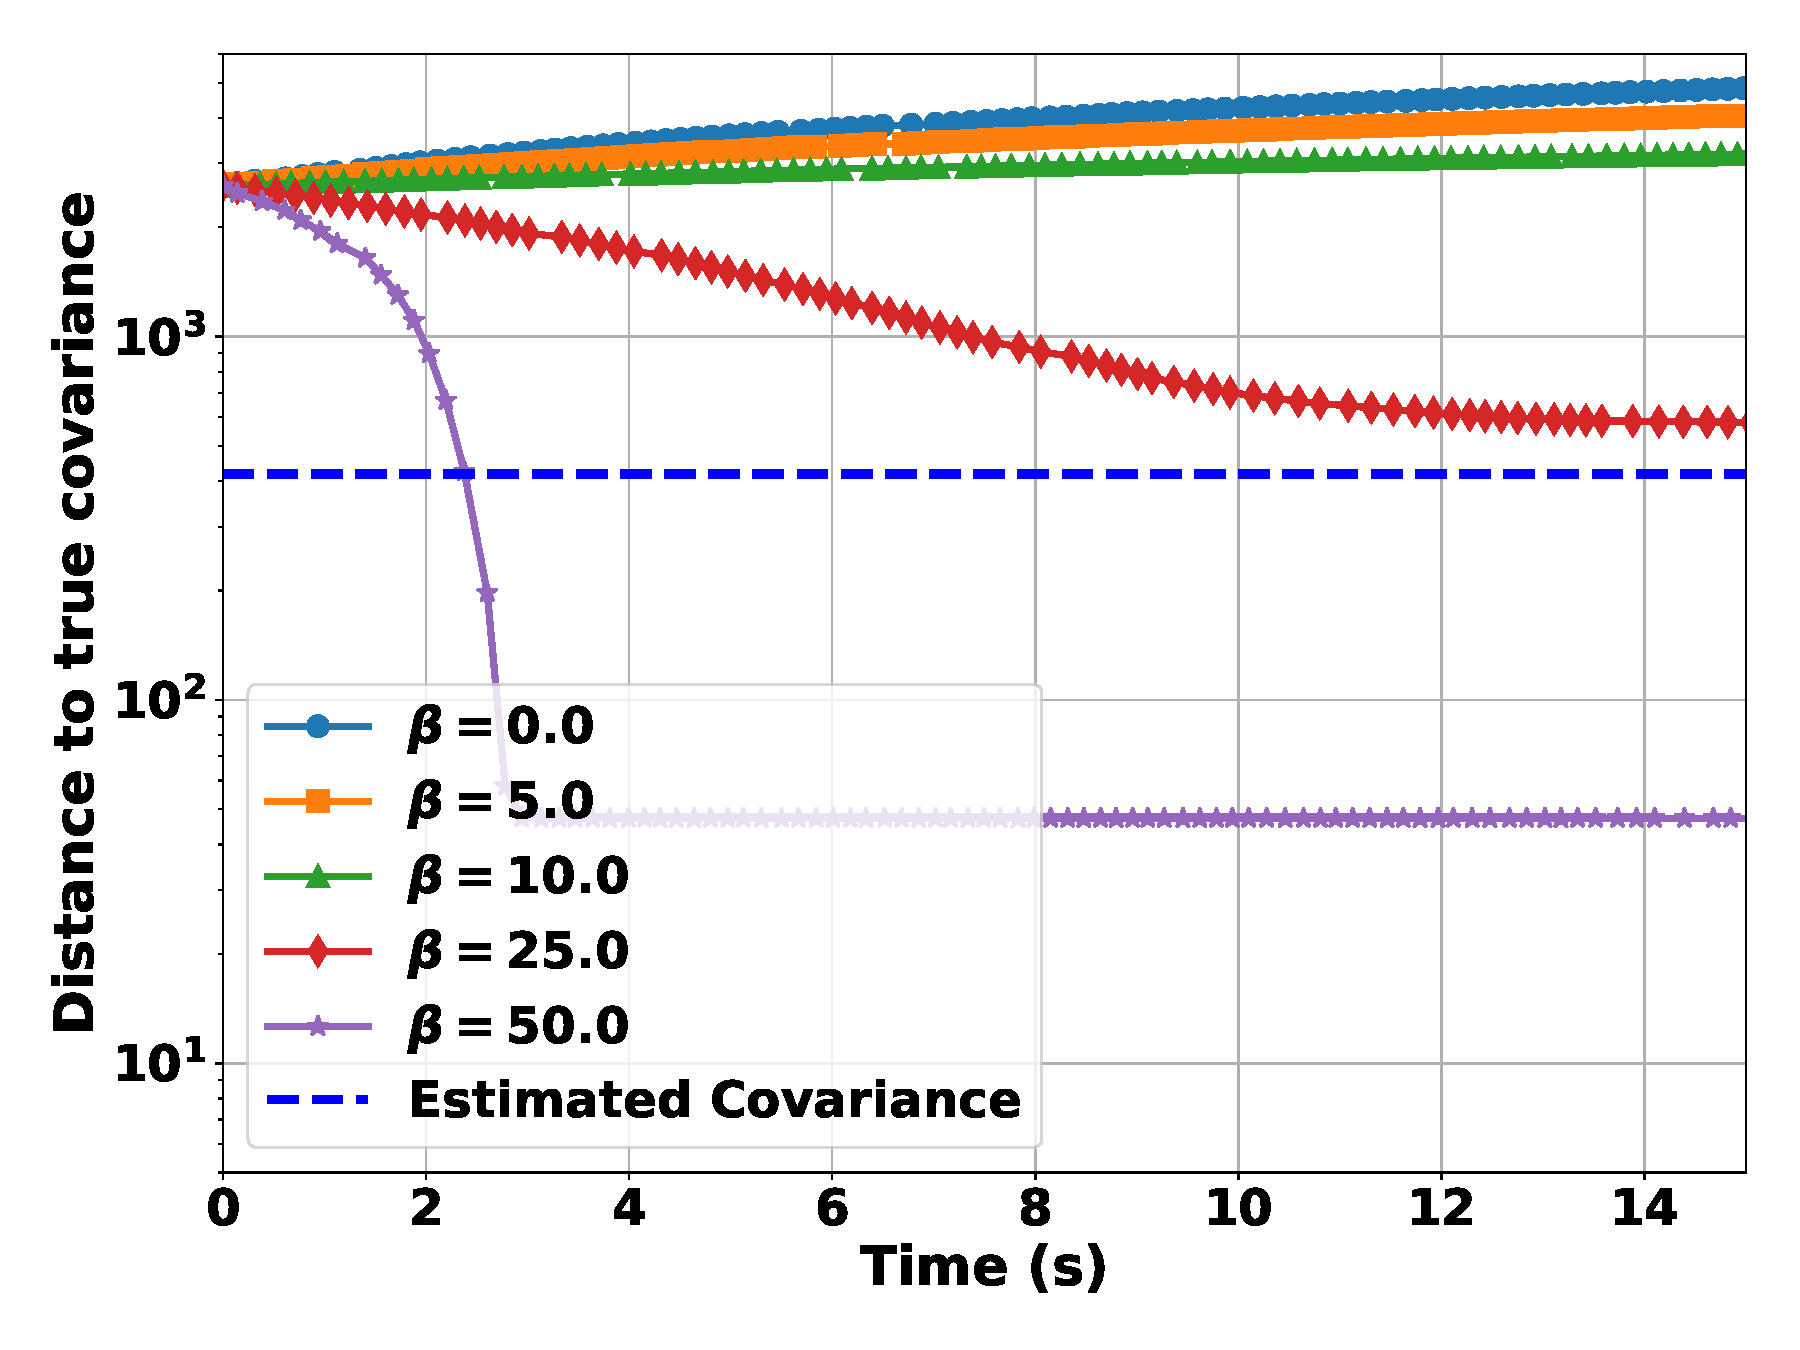
\includegraphics[width=0.43\linewidth]{figuresV2/multivar_t/t_aux_nu5_d30_n1500.pdf}
    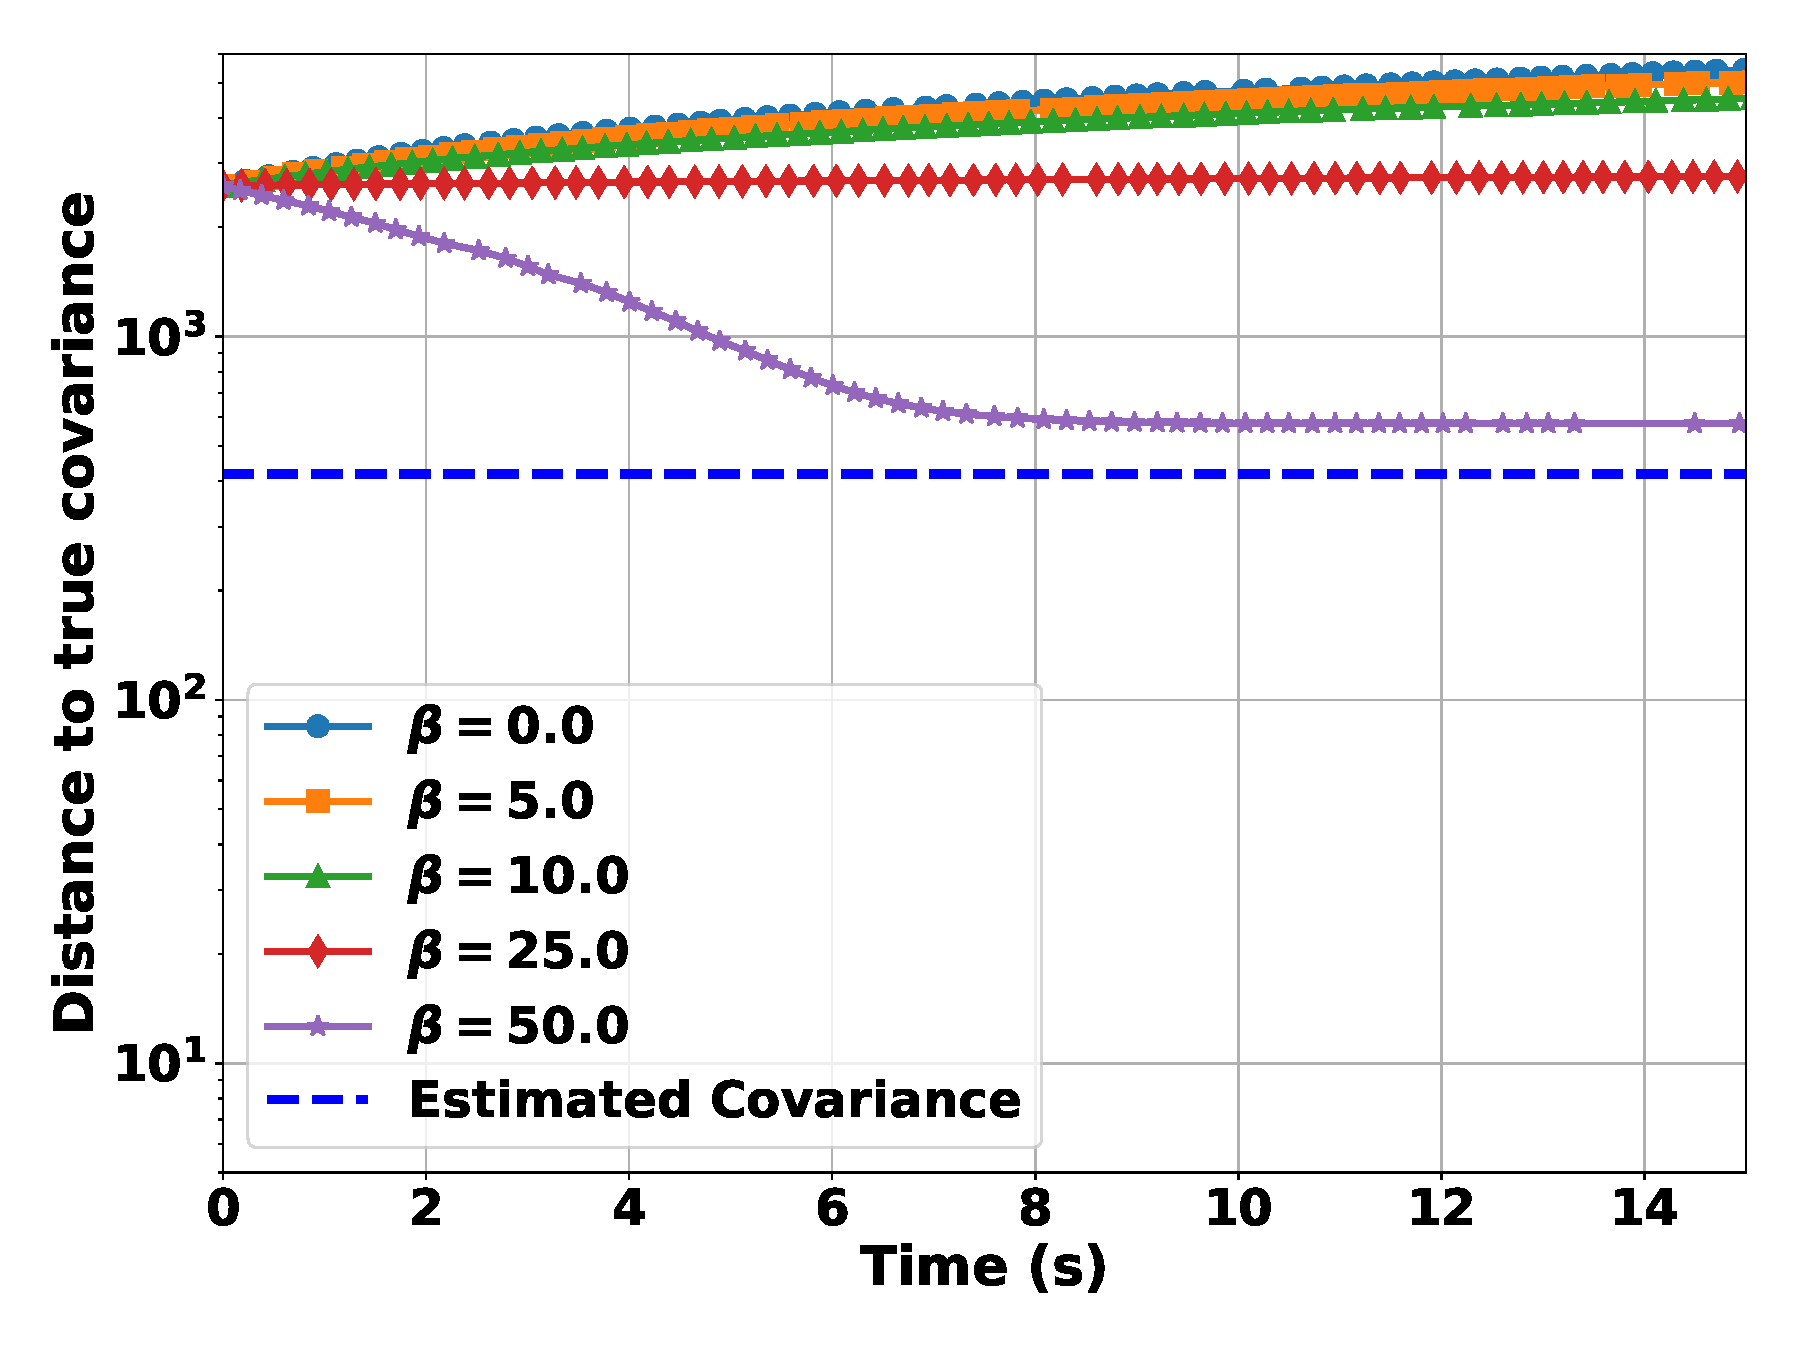
\includegraphics[width=0.43\linewidth]{figuresV2/multivar_t/t_aux_nu5_d30_n3000.pdf}
    \caption{\textbf{Multivariate T-Distribution Optimistic Likelihood.} Both plots are $d=30$ and $\nu = 5$. The left plot is generated with $n=1500$ and the right with $n=3000$. This method requires a high number of samples for it to correspond with the theory. In particular, the right-side plot agreees with the theory: higher regularization corresponds to closer solutions to $\hat{\Sigma}$ in a monotonic fashion. The left-hand side with insufficient data points violates this.}
    \label{fig:multivar_t_aux_high_samples}
\end{figure}







% Also, we will demonstrate the performance of CCCP, i.e., the fixed point algorithm~\ref{eq:inverse_fp} on the following problem 

% \begin{equation}
%     \min_{P \in \pd} \left\{ \hat\phi(P) \defas \tr(P S) - \log \det P + \beta \delta_S^2(P,\hat{P}) \right\}.
% \end{equation}
% This problem was also introduced in Section~\ref{sec:GaussianMLE_intro} can arises after making the variable substitution $P = \Sigma^{-1}$ of Problem~\ref{exp:sdiv_ball_MLE_Problem}.









% \begin{table}[h!]
% \centering
% \begin{tabular}{|c|c|c|}
% \hline
% $\beta$ & $\|\Sigma^* - S\|_F$ & $\|\hat{\Sigma} - \hat{\Sigma}\|_F$ \\ \hline
% 0  & 21.741  & 780.233 \\ \hline
% 1  & 231.662 & 566.262 \\ \hline
% 2  & 351.602 & 446.663 \\ \hline
% 10 & 617.255 & 180.798 \\ \hline
% \end{tabular}
% \caption{$\Sigma^*$ denotes the output of Algorithm~\ref{alg:CCCP_on_MLE} with varying regularization parameter $\beta$ for $n=1500$ and $d=100$.}
% \label{table:gaussian_aux_norm_100}
% \end{table}



% \ac{Todo: Mention that log-normal is also g-cvx + DC and probably a subclass of log elliptically contoured distributions are as well.
% Maybe provide the fixed point algorithm as well.
% }



% \begin{itemize}
%      \item CCCP algorithm: Why DC structure is favourable/exploited algorithmically
%      \item Recipes for solving CCCP routine 
%      \item Structured Relaxation
%      \item modular structure lends itself to our DGP program
% \end{itemize}

% \paragraph{Examples of G-Cvx+DC Problems.}
% \begin{itemize}
%     \item Karcher Mean (and square root)
%     \item Tyler's M-Estimator
%     \item Brascamp-Lieb?
%     \item Optimistic Likelihood Calculation?
% \end{itemize}

% \section{Applications}
% List some other problems that can potentially fall into our setting
% \begin{itemize}
%     \item Pure regularization
%     \item Likelihood estimation: See Section 8.3 of Winter Journal Part I for more intuition of using S-divergence as a regularizer. 
%     \item Each problem have a experiment graph 
% \end{itemize}

%%%%%%%%%%%%%%%%%%%%%%%%%
\section{Discussion}
In this paper we introduced structured regularization approaches for constrained optimization on the SPD manifold. We considered different classes of constraints with a particular focus on sparsity and ball constraints. Our structured regularization approach relies on symmetric gauge functions, whose algebraic properties give rise to a modular framework that allows for designing regularizers that preserve desirable properties of the orginial objective, specifically geodesic convexity and difference of convex structure. We illustrate the utility of our approach on a range of data science and machine learning applications.

We believe that our proposed approach opens up new directions for constrained optimization on Riemannian manifolds that circumvents the potentially costly subroutines of standard constrained Riemannian optimization approaches, such as R-PGD and R-FW. While we focus on two specific classes of constraints for most of the paper, we believe that our approach could be applied much more broadly. Our discussion on disciplined programming with symmetric gauge functions may serve as a starting point for future work in this direction. The introduction of new regularizers for structured constraints could significantly widen the range of applications in machine learning and data science. Furthermore, while this paper only discusses constrained optimization on the SPD manifold, we believe that many of the ideas could be extended to other Cartan-Hadamard manifolds.


%%%%%%%%%%%%%%%%%%%%%%%%
\section*{Acknowledgements}
We thank Bobak Kiani and Vaibhav Dixit for helpful discussions and comments.\\ 

\noindent This work was supported by the Harvard Dean’s Competitive Fund for Promising Scholarship and NSF award 2112085. AC is partially supported by a NSERC Postgraduate Fellowship.

%%%%%%%%%%%%%%%%%%%%%%%%%
%\pagebreak
\bibliography{notes_template/refs}
% \bibliographystyle{plain}
\bibliographystyle{alpha}

%%%%%%%%%%%%%%%%%%%%%%%%
\newpage
%\section{Appendix}






%\section{Figures}
%\subsection{Square Root.}
%The following is $200 \times 200$ matrices in the mediuum-conditioned case \\
%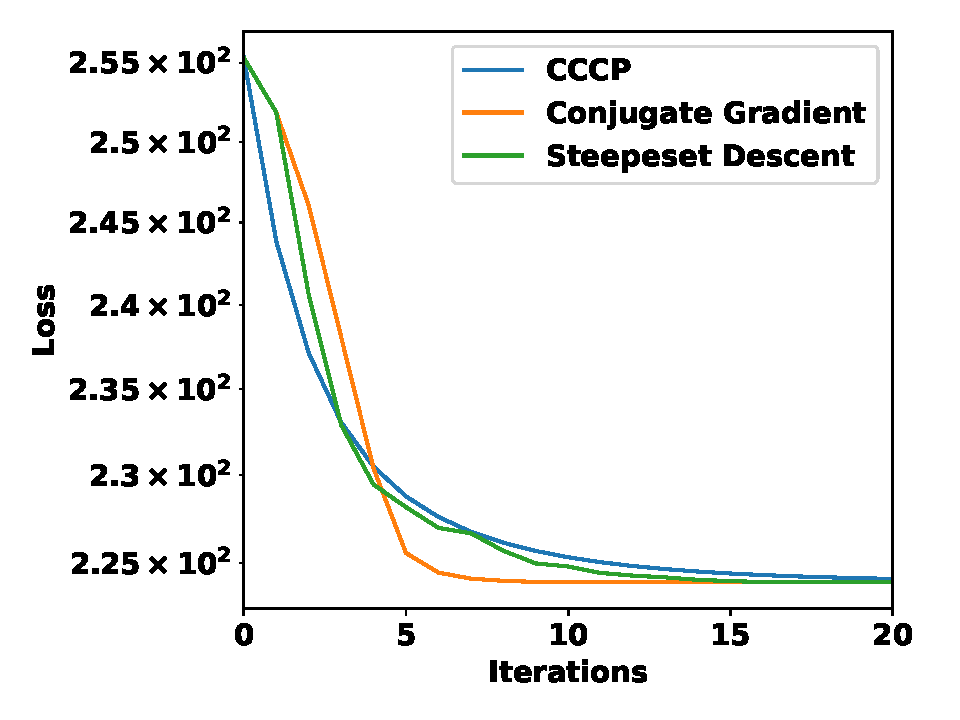
\includegraphics[height=6.3cm]{figuresV2/square_root/loss_iter_200_medium.pdf}
%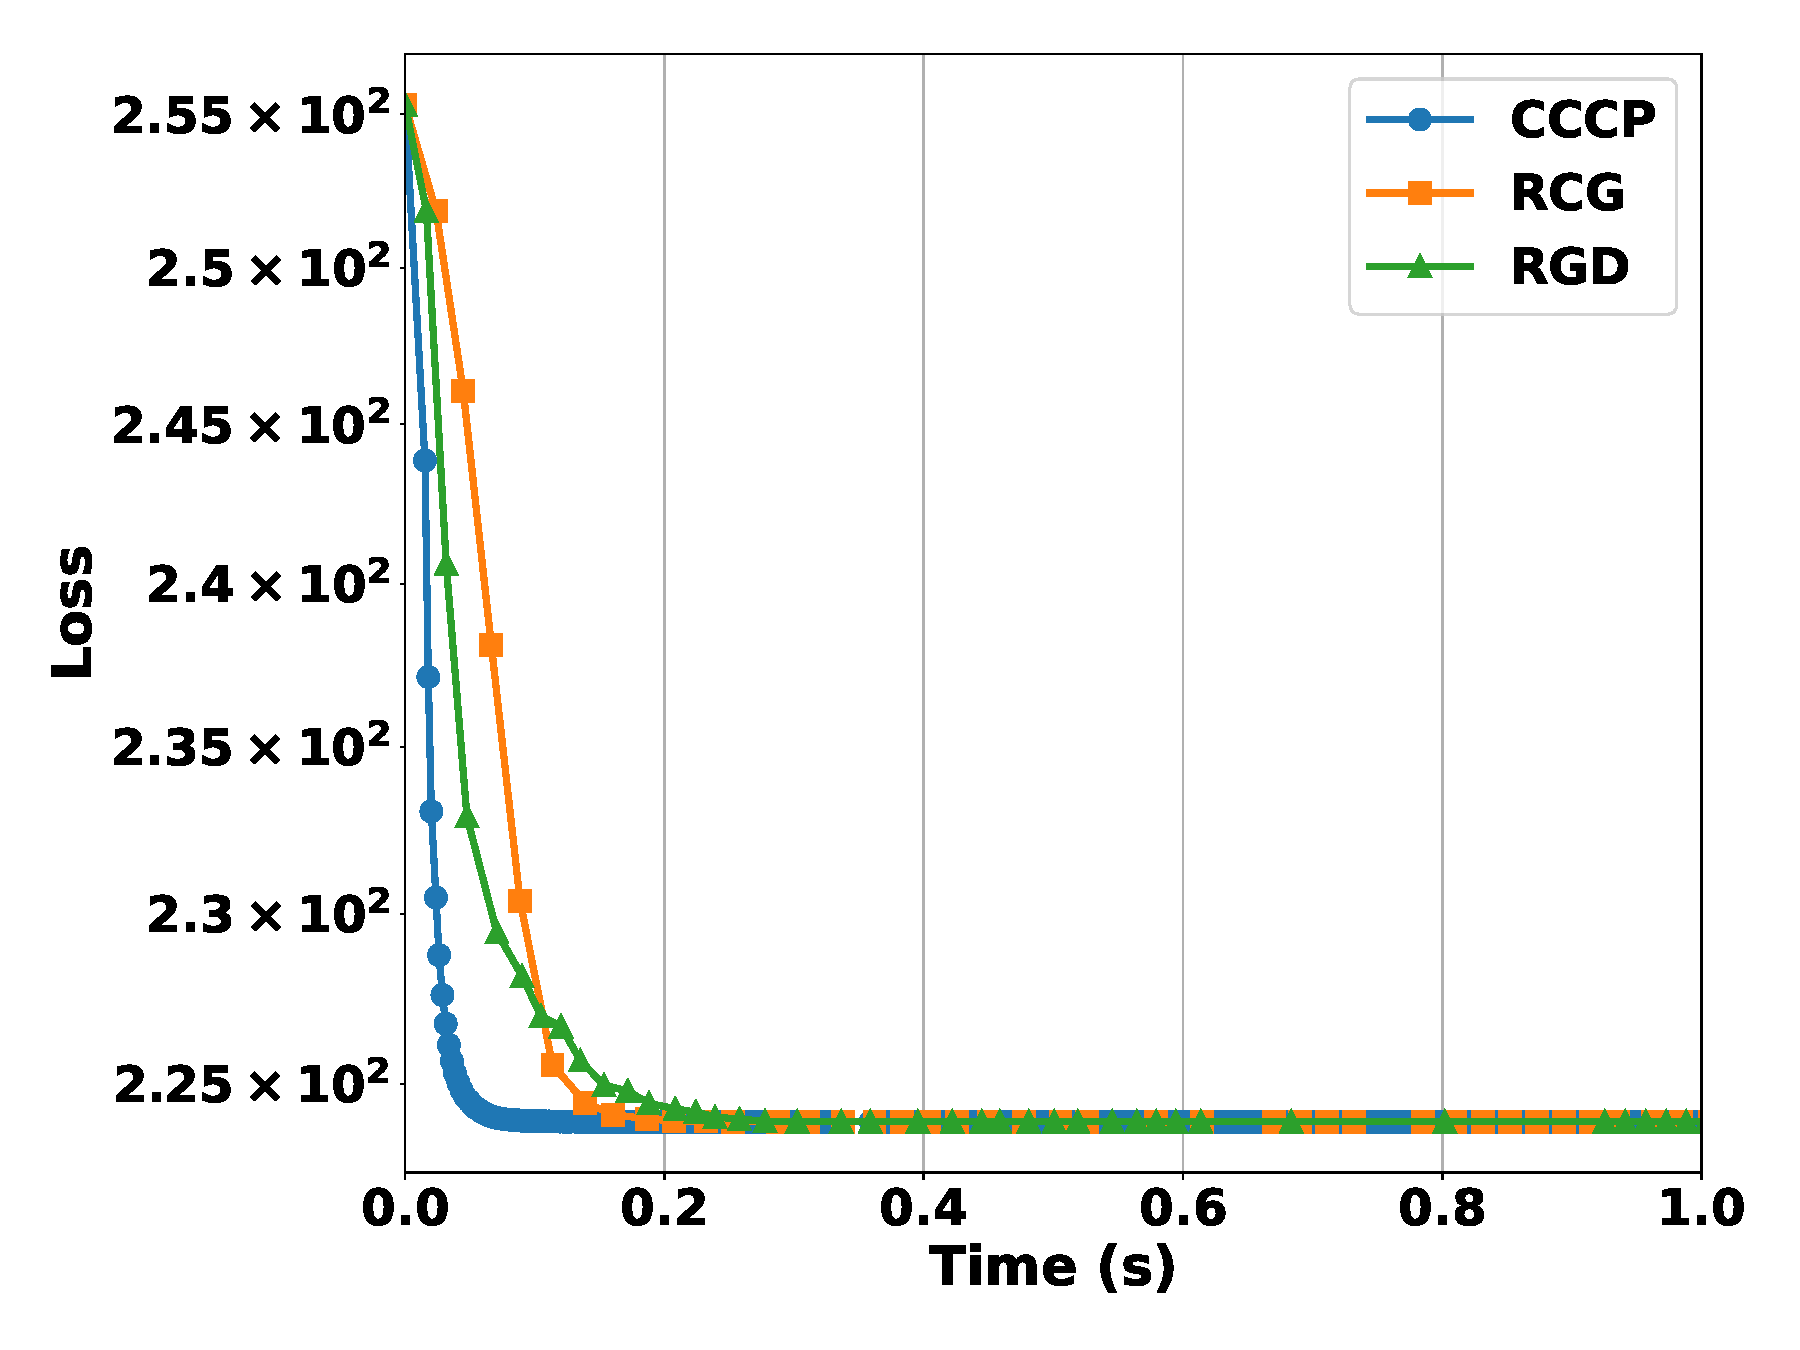
\includegraphics[height=6.3cm]{figuresV2/square_root/loss_time_200_medium.pdf} \\
%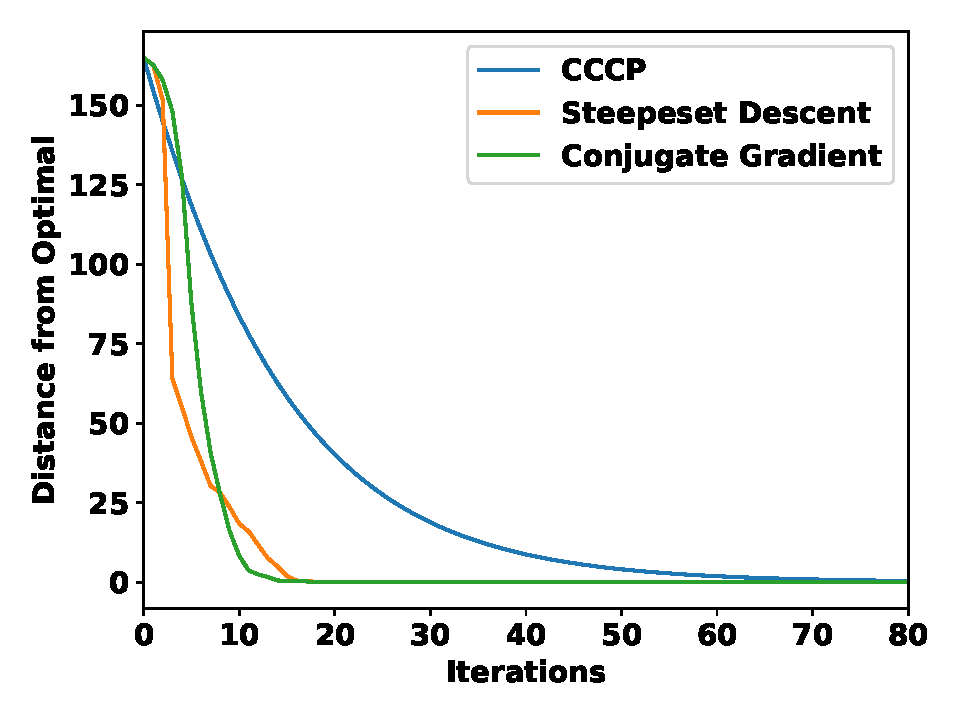
\includegraphics[height=6.3cm]{figuresV2/square_root/distance_iter_200_medium.pdf}
%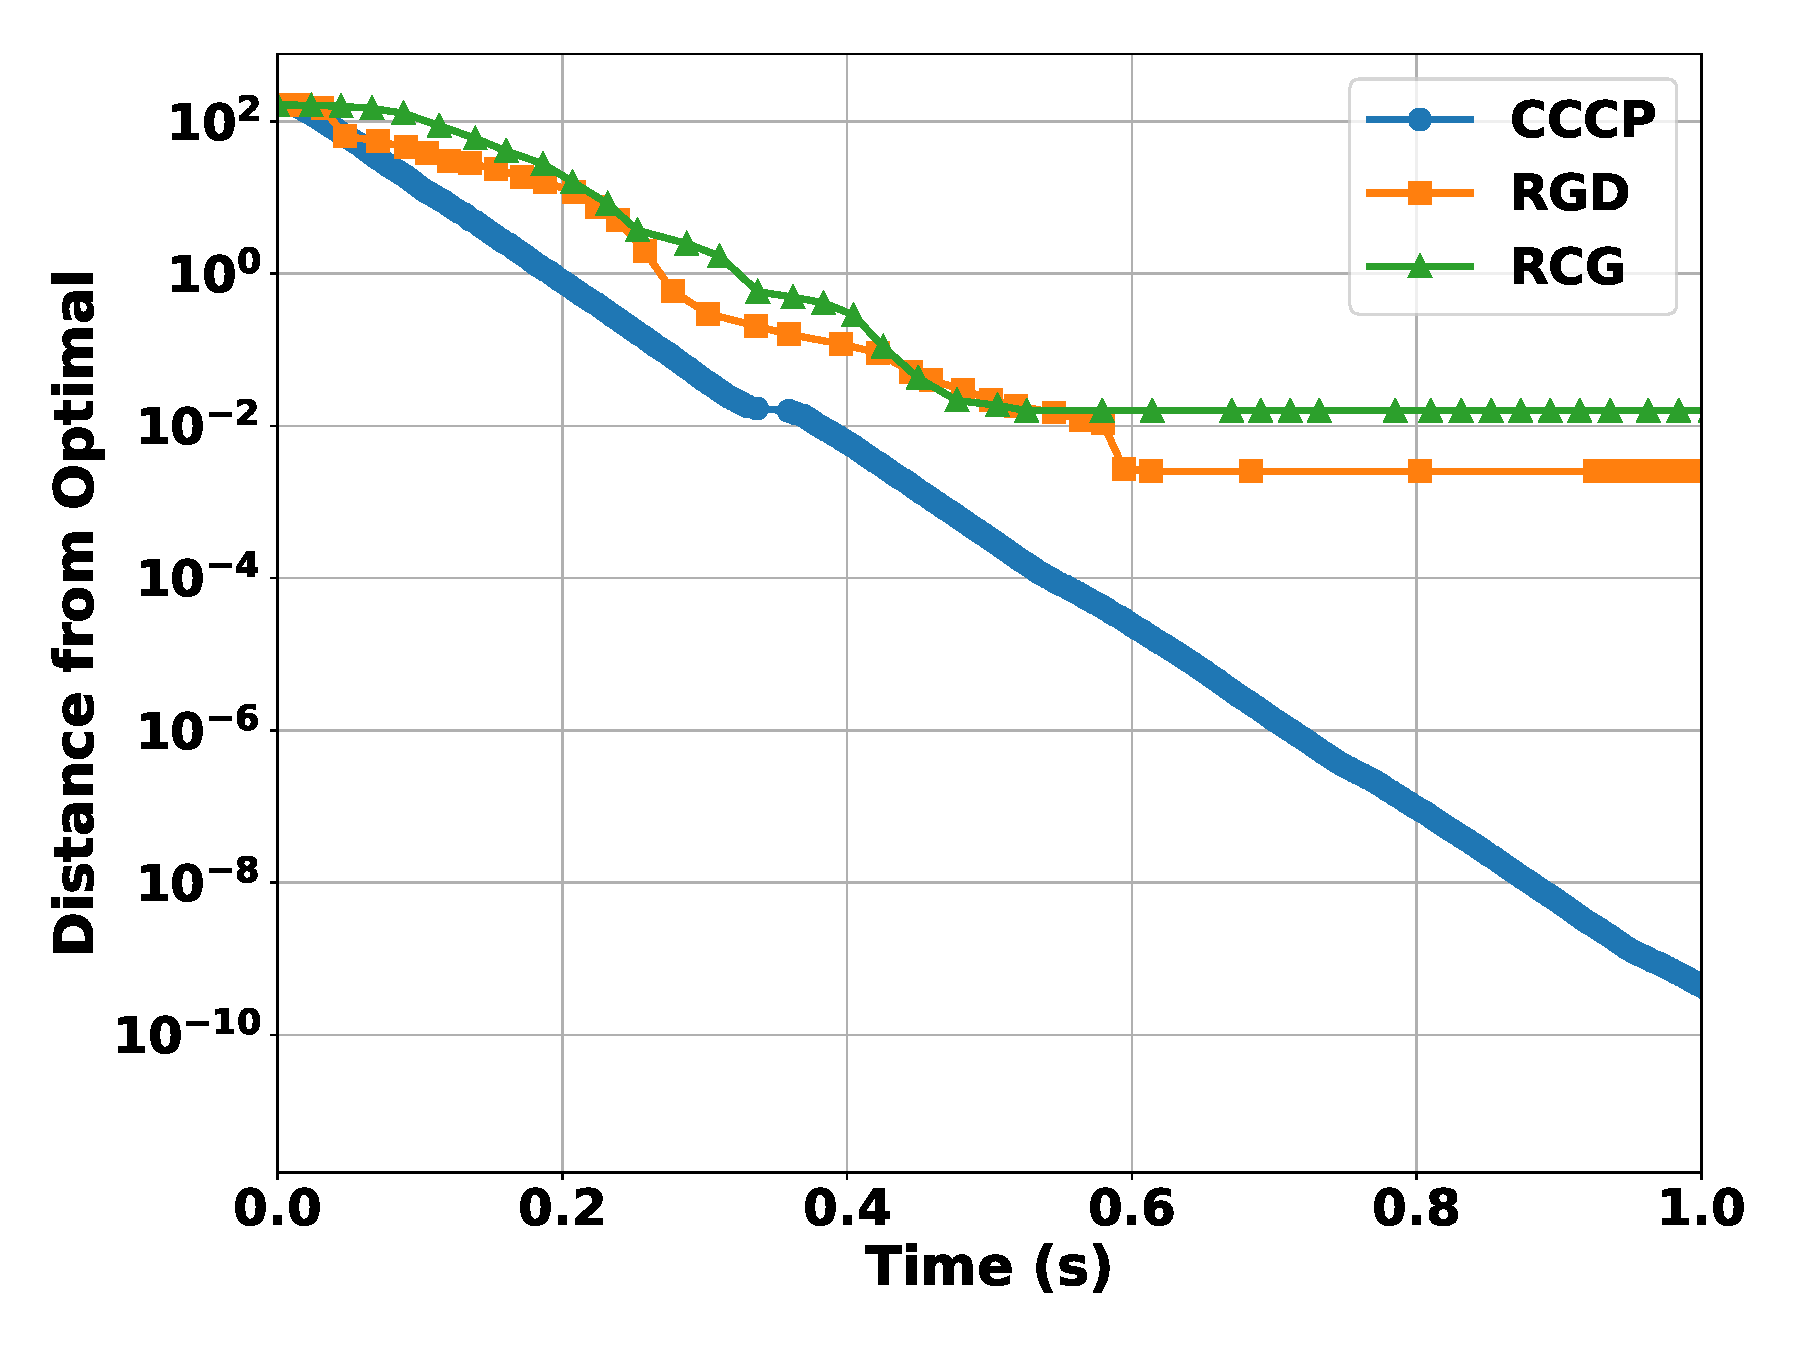
\includegraphics[height=6.3cm]{figuresV2/square_root/distance_time_200_medium.pdf}\\

%\textbf{Ill-Conditioned.} Computing the square root of the $200 \times 200$ Hilbert matrix. 
%\\



%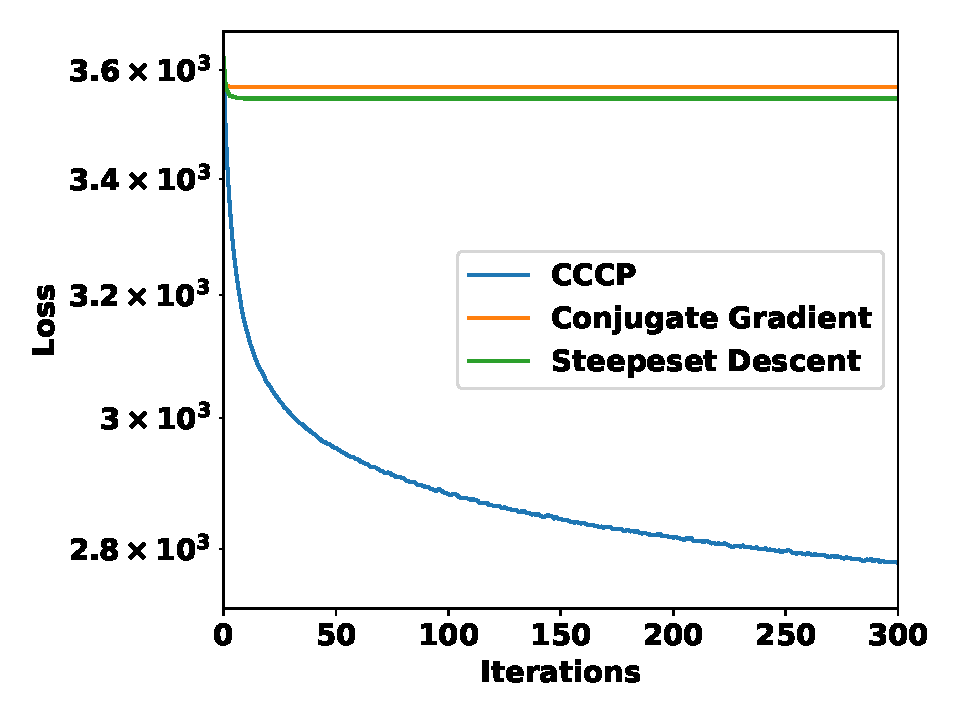
\includegraphics[height=6.3cm]{figuresV2/square_root/loss_iter_200_ill.pdf}
%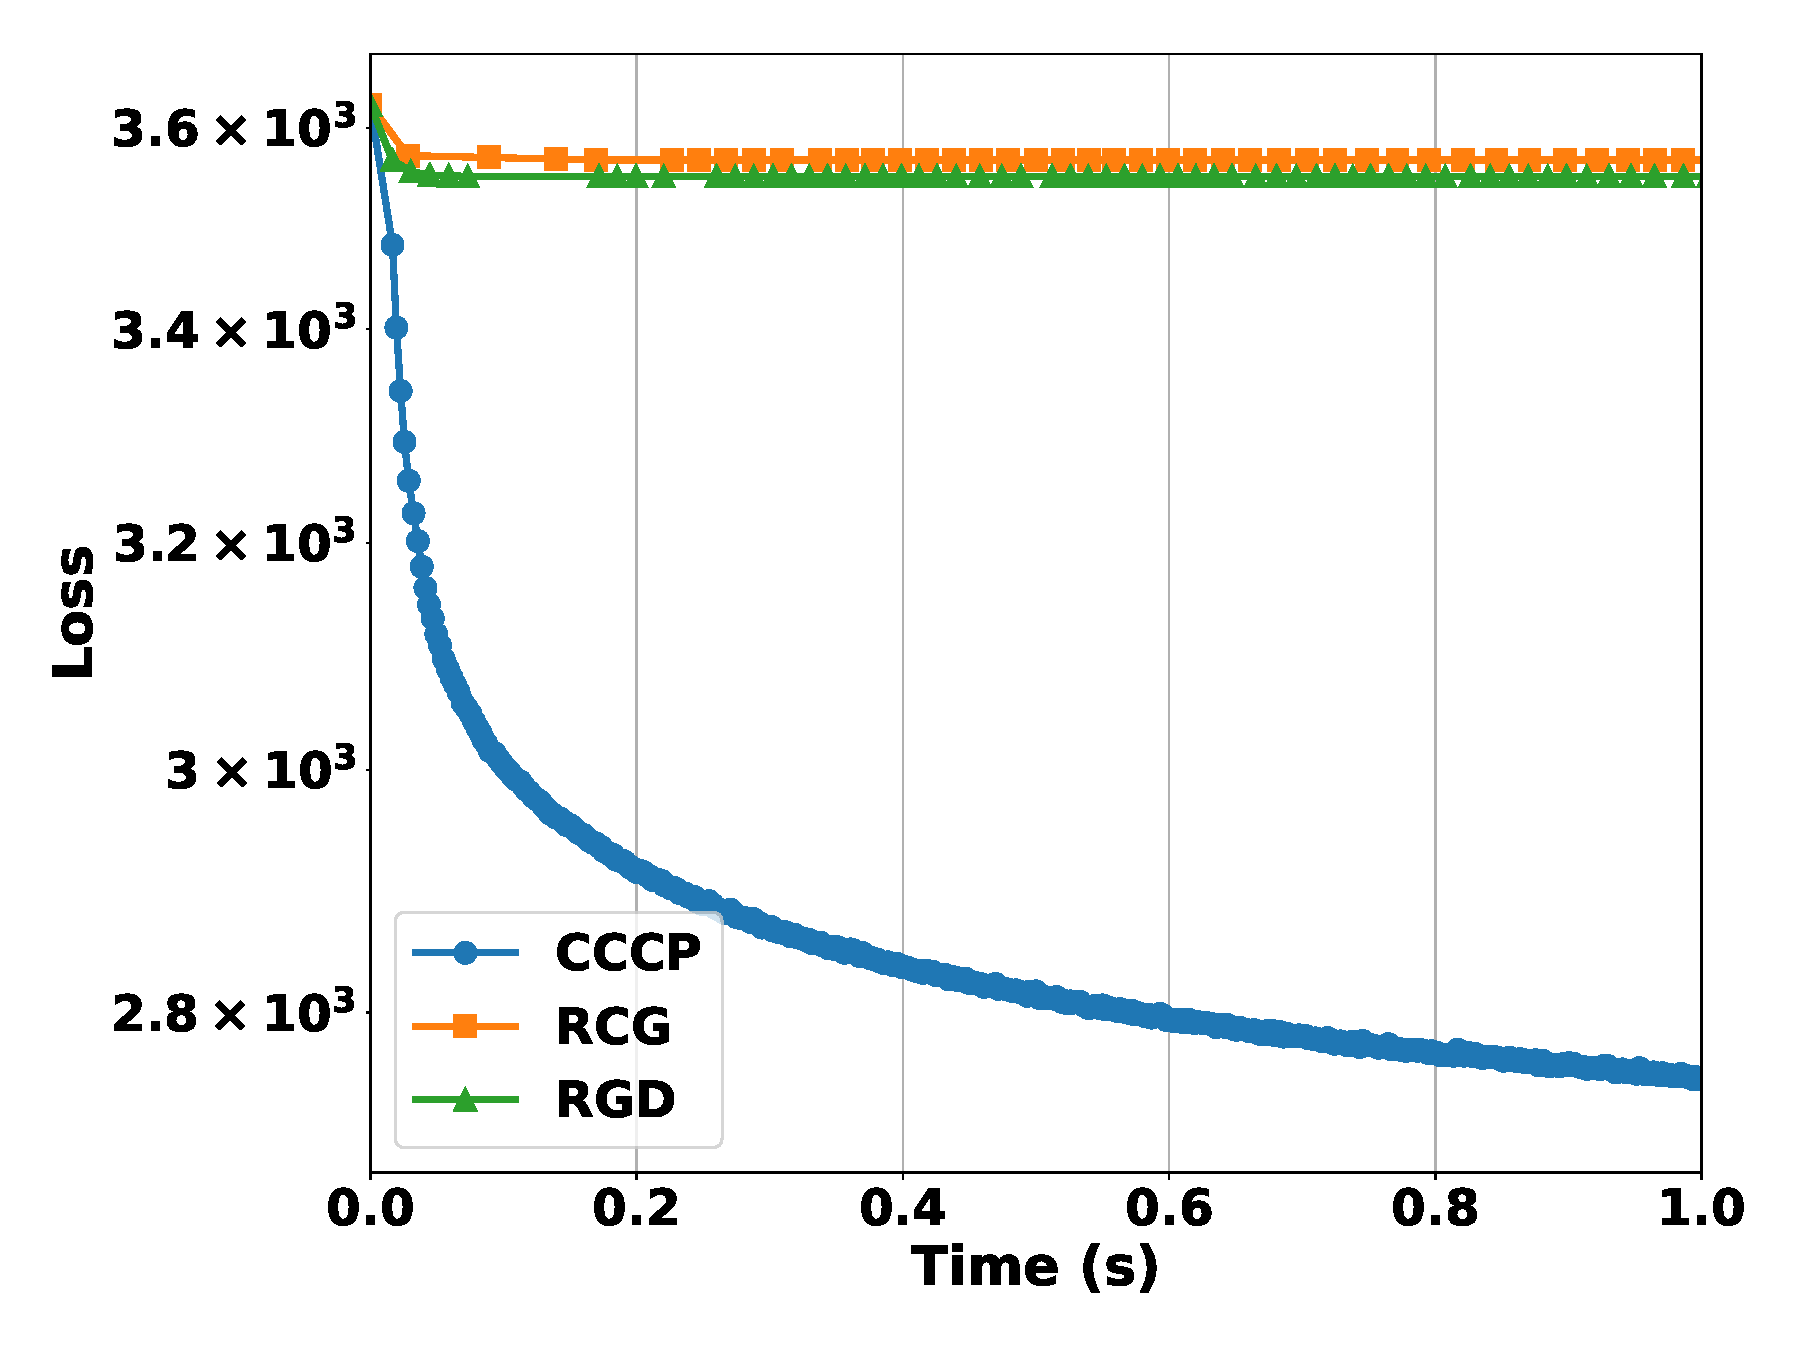
\includegraphics[height=6.3cm]{figuresV2/square_root/loss_time_200_ill.pdf} \\
%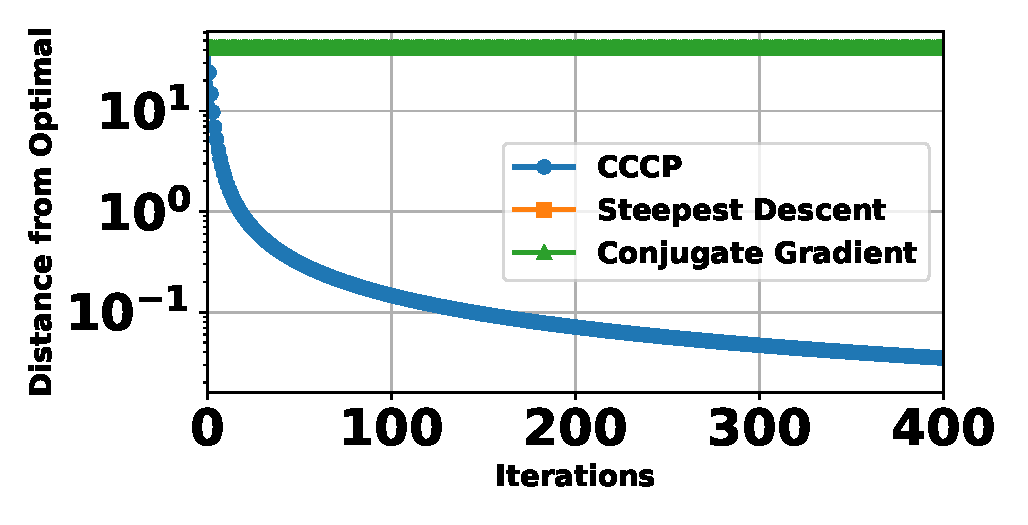
\includegraphics[height=6.3cm]{figuresV2/square_root/distance_iter_200_ill.pdf}
%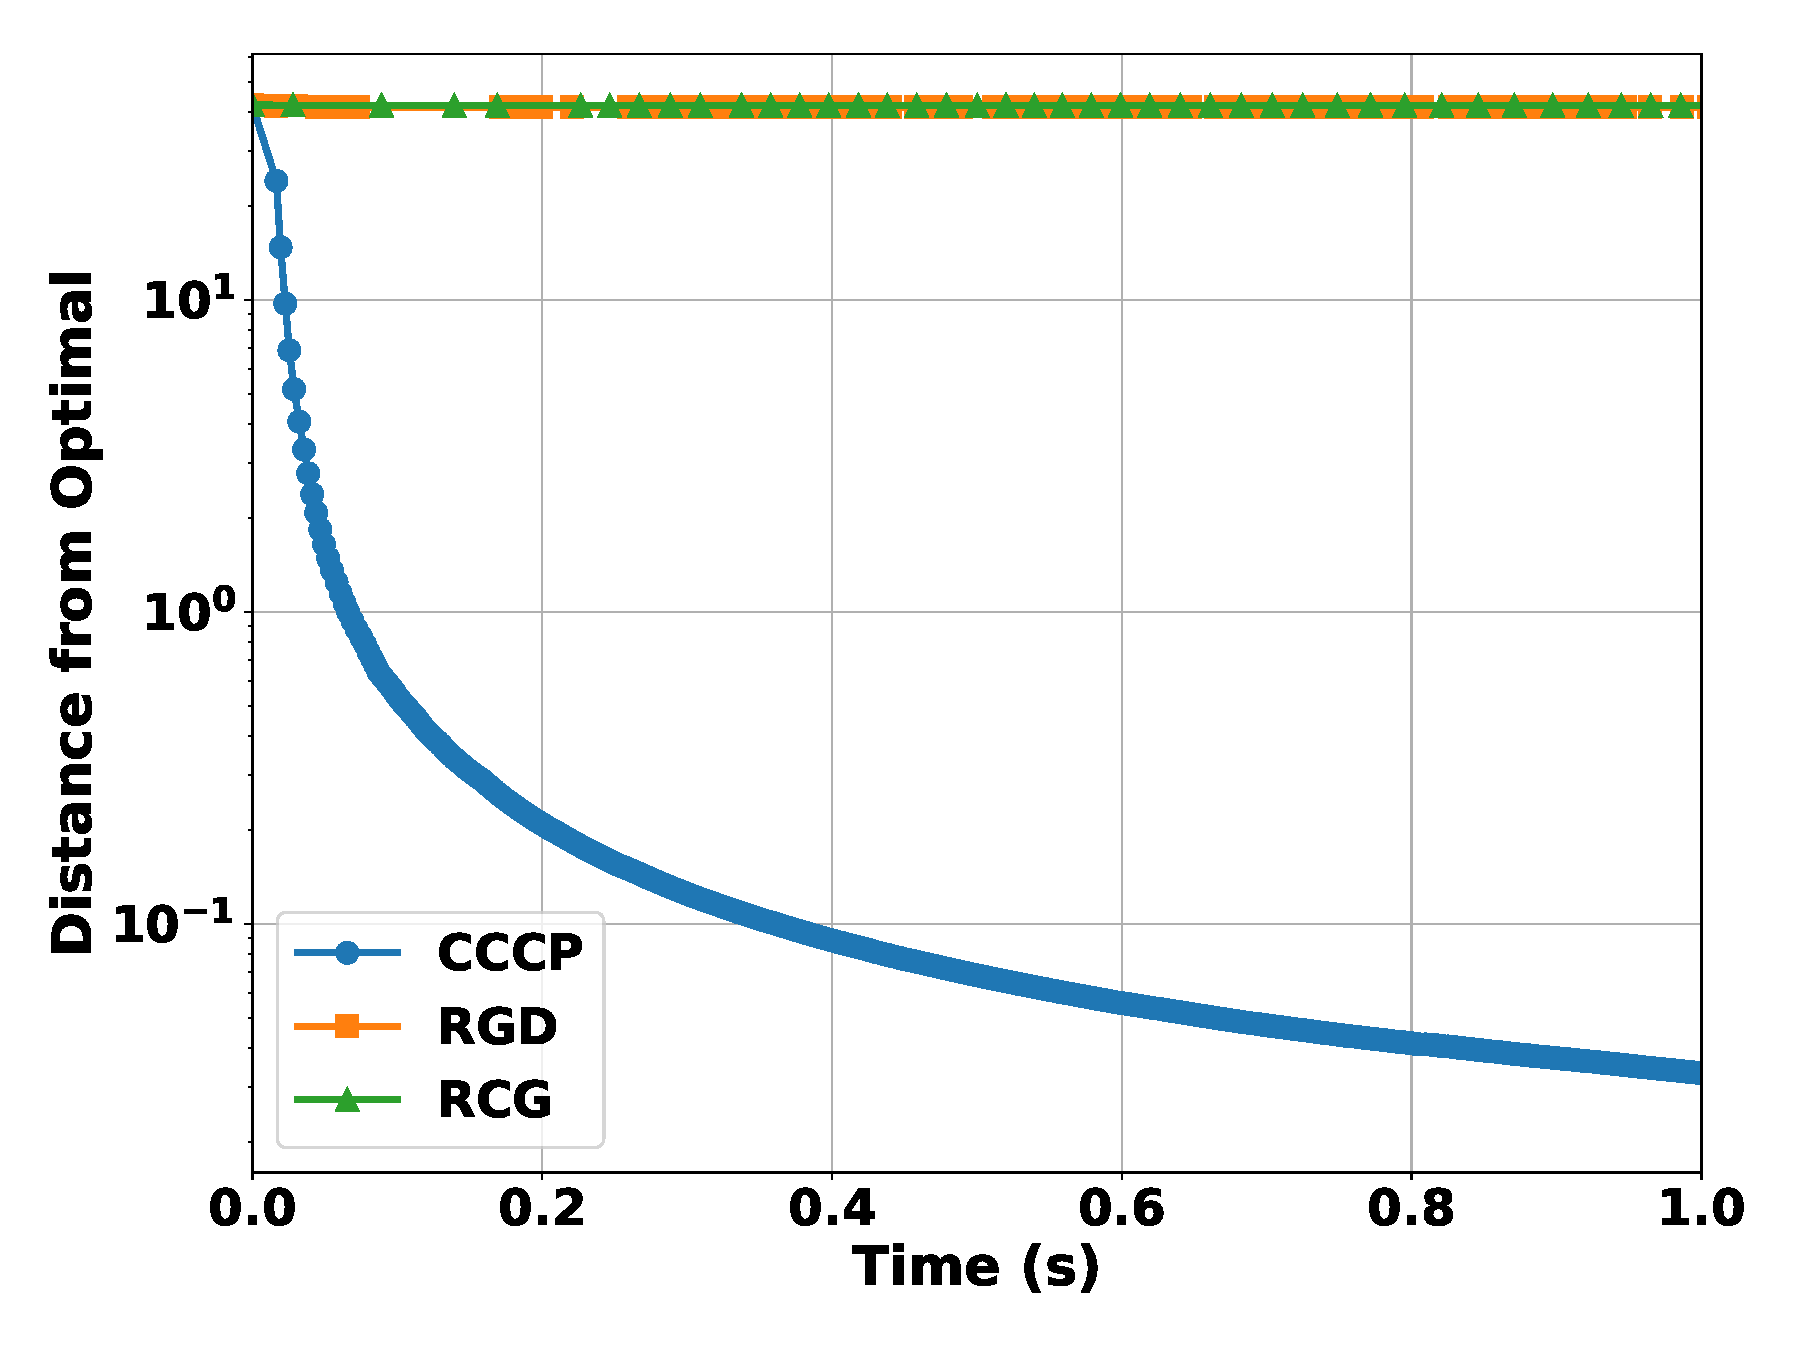
\includegraphics[height=6.3cm]{figuresV2/square_root/distance_time_200_ill.pdf}


%\paragraph{Frobenius distance from last iterate on Hilbert Matrices} 
%We each algorithm for $K=400$ iterations.  Denote the output of each algorithm by $X_{400}$. Denote $\hat{H}_{\operatorname{CCCP}}  = X_{400}^2$ the reconstruction of the $200 \times 200$ Hilbert matrix $H$ using the output of the CCCP algorithm. Also, denote $\hat{H}_{\operatorname{SD}}$ and $\hat{H}_{\operatorname{CG}}$ in the same manner with their corresponding last iterates. We have that 
%\[
%\begin{aligned}
%    &\|H - \hat{H}_{\operatorname{CCCP}}\|_{F} = 8.9 \times 10^{-5}
%    \\&\|H - \hat{H}_{\operatorname{SD}}\|_{F} = 129.791
%    \\&\|H - \hat{H}_{\operatorname{CG}}\|_{F} = 126.335 
%\end{aligned}
%\]
%where $H$ denotes the $200 \times 200$ Hilbert matrix.

%\subsection{Karcher Mean}

%\textbf{Medium Conditioned.} $m =100$ and $100 \times 100$ matrices. The optimal is taken to be the average of the last iterate of the three algorithms upon convergence.

%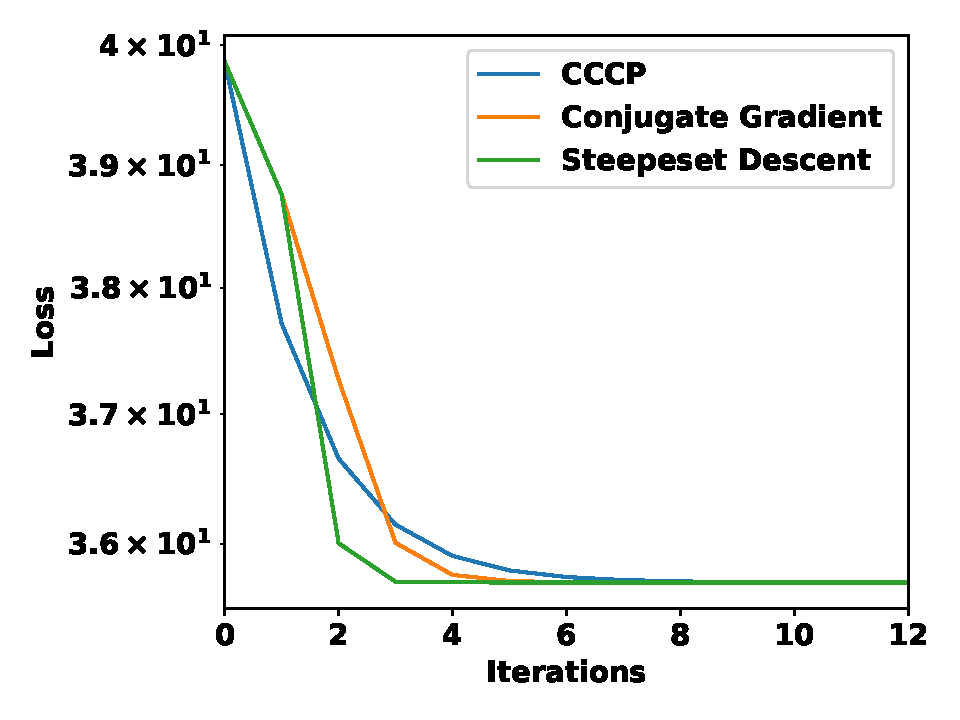
\includegraphics[height=6.3cm]{figuresV2/karcher_mean/loss_iter_100_100_medium.pdf}
%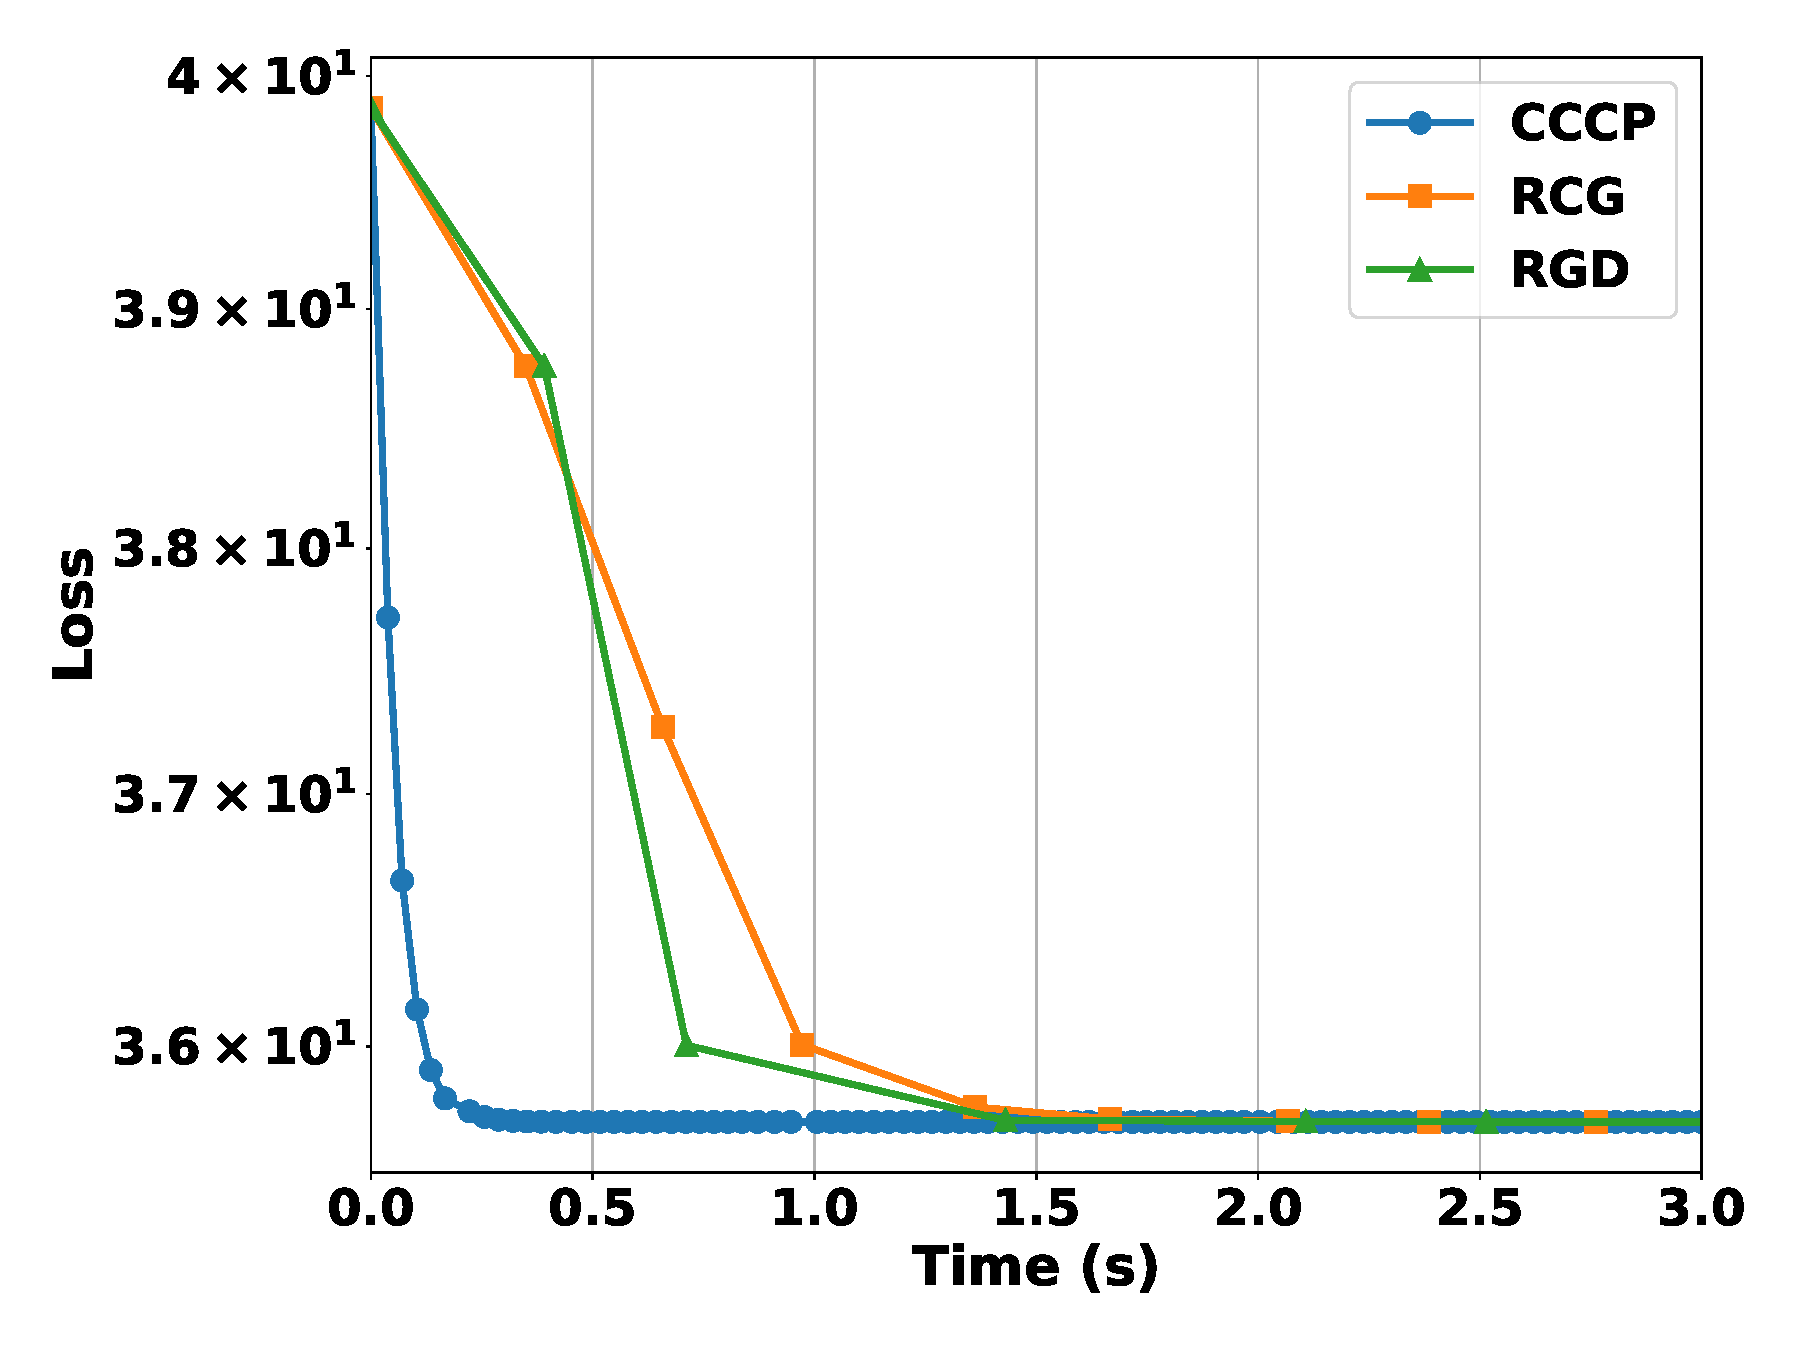
\includegraphics[height=6.3cm]{figuresV2/karcher_mean/loss_time_100_100_medium.pdf}\\
%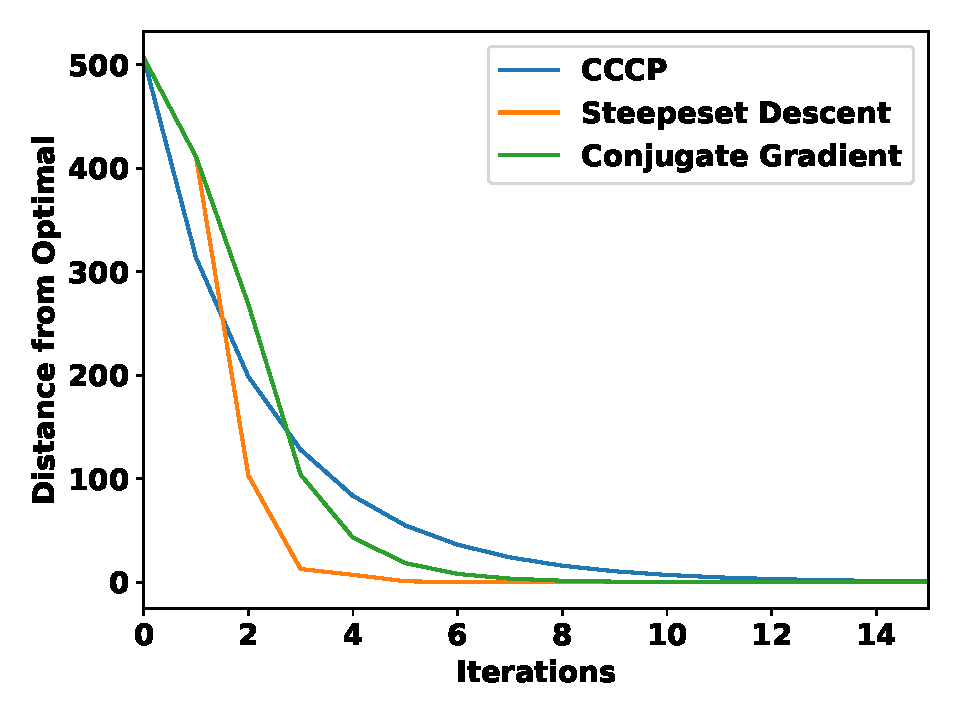
\includegraphics[height=6.3cm]{figuresV2/karcher_mean/distance_iter_100_100_medium.pdf}
%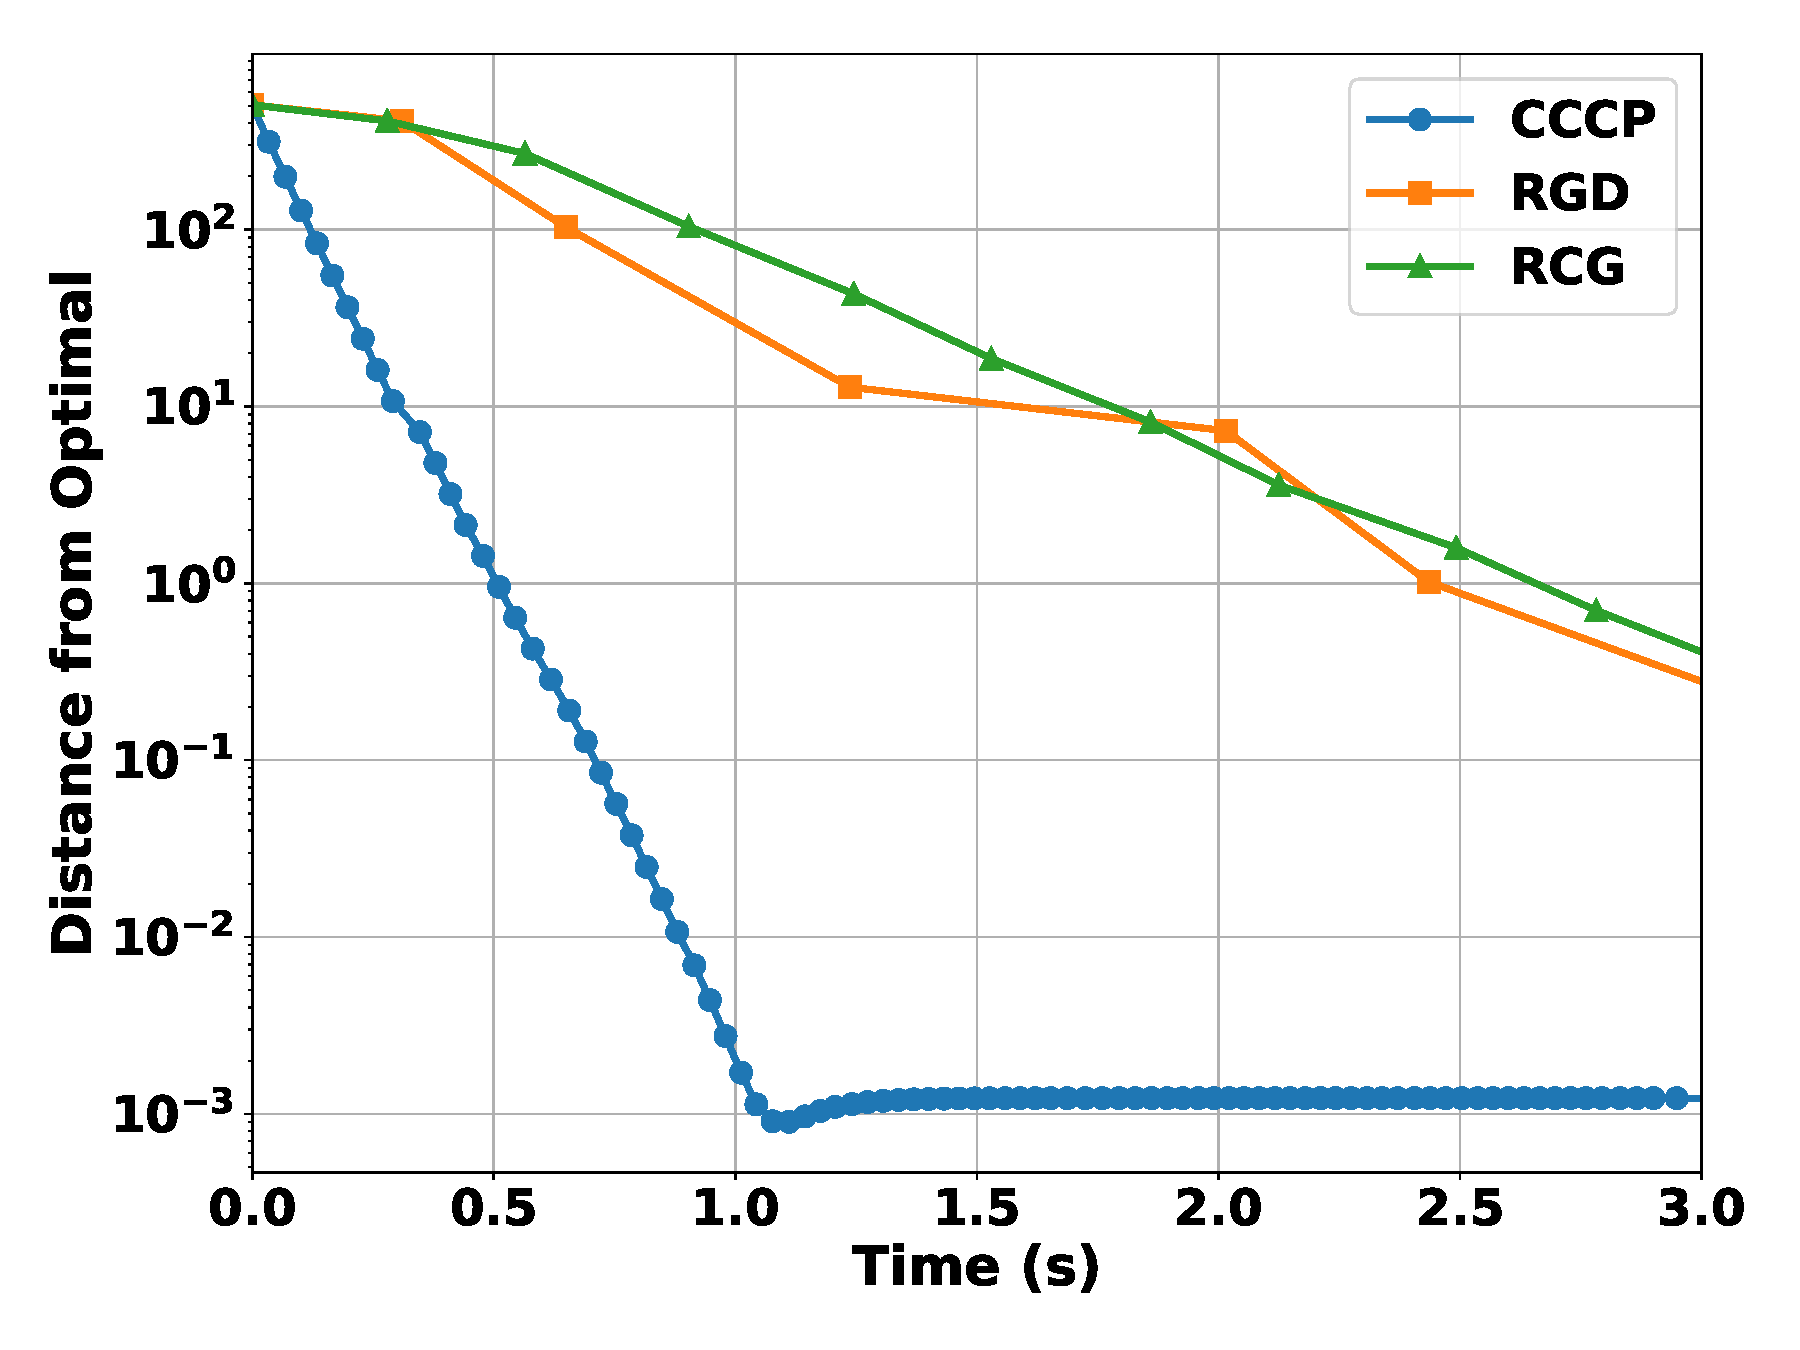
\includegraphics[height=6.3cm]{figuresV2/karcher_mean/distance_time_100_100_medium.pdf}

% Now we take $m=200$ and $100 \times 100$ matrices. 


% 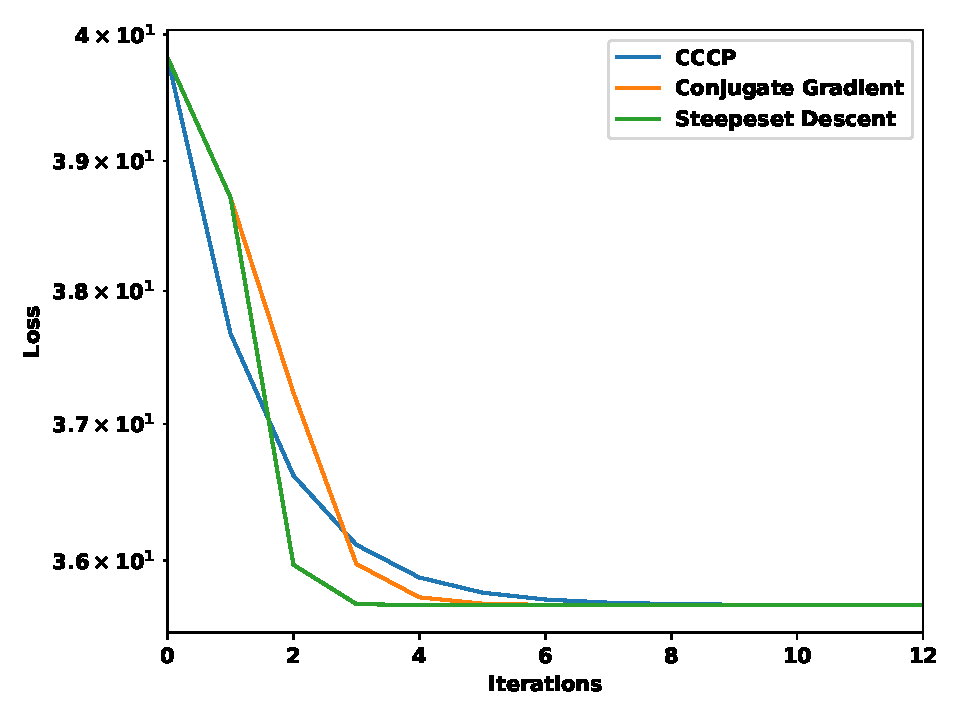
\includegraphics[height=6.3cm]{figuresV2/karcher_mean/loss_iter_200_100_medium.pdf}
% \includegraphics[height=6.3cm]{figuresV2/karcher_mean/loss_time_200_100_medium.pdf}\\
% \includegraphics[height=6.3cm]{figuresV2/karcher_mean/distance_iter_200_100_medium.pdf}
% \includegraphics[height=6.3cm]{figuresV2/karcher_mean/distance_time_200_100_medium.pdf}


%Now we take $m=500$ and $100 \times 100$ matrices. 


%\includegraphics[height=6.3cm]%{figuresV2/karcher_mean/loss_iter_500_100_medium.pdf}
%\includegraphics[height=6.3cm]{figuresV2/karcher_mean/loss_time_500_100_medium.pdf}\\
%\includegraphics[height=6.3cm]{figuresV2/karcher_mean/distance_iter_500_100_medium.pdf}
%\includegraphics[height=6.3cm]{figuresV2/karcher_mean/distance_time_500_100_medium.pdf}

%\subsection{Gaussian MLE}


% \begin{table}[h!]
% \centering
% \begin{tabular}{|c|c|c|}
% \hline
% $\beta$ & $\|\Sigma^* - S\|_F$ & $\|\Sigma^* - \hat{\Sigma}\|_F$ \\ \hline
% 0  & 0.149   & 412.009 \\ \hline
% 1  & 116.545 & 296.022 \\ \hline
% 2  & 178.140 & 234.583 \\ \hline
% 10 & 316.485 & 96.094  \\ \hline
% \end{tabular}
% \caption{$\Sigma^*$ denotes the output of Algorithm~\ref{alg:CCCP_on_MLE} with varying regularization parameter $\beta$ for $n=100$ and $d =30$}
% \label{table:gaussian_aux_norm_30}
% \end{table}



% \begin{table}[h!]
% \centering
% \begin{tabular}{|c|c|c|}
% \hline
% $\beta$ & $\|\Sigma^* - S\|_F$ & $\|\hat{\Sigma} - \hat{\Sigma}\|_F$ \\ \hline
% 0  & 21.741  & 780.233 \\ \hline
% 1  & 231.662 & 566.262 \\ \hline
% 2  & 351.602 & 446.663 \\ \hline
% 10 & 617.255 & 180.798 \\ \hline
% \end{tabular}
% \caption{$\Sigma^*$ denotes the output of Algorithm~\ref{alg:CCCP_on_MLE} with varying regularization parameter $\beta$ for $n=1500$ and $d=100$.}
% \label{table:gaussian_aux_norm_100}
% \end{table}



% \includegraphics[height=6cm]{figuresV2/Gaussian_MLE/cccp_gaussianMLE_100.pdf}

% \[
% \begin{aligned}
%     &\|\hat{\Sigma}_{0} - S \|_F = 21.706120575132054 \\
%     &\|\hat{\Sigma}_{1} - S \|_F = 231.66649127504314 \\
%     &\|\hat{\Sigma}_{2} - S \|_F = 351.60624106643934 \\
%     &\|\hat{\Sigma}_{10} - S \|_F = 617.2565242338849 \\
% \end{aligned}
% \]

% \[
% \begin{aligned}
%     &\|\hat{\Sigma}_{0} - \hat{\Sigma} \|_F = 780.2332561880564\\
%     &\|\hat{\Sigma}_{1} - \hat{\Sigma} \|_F = 566.2625281295786 \\
%     &\|\hat{\Sigma}_{2} - \hat{\Sigma} \|_F = 446.66284393546135 \\
%     &\|\hat{\Sigma}_{10} - \hat{\Sigma} \|_F = 180.79832430792698\\
% \end{aligned}
% \]


%\subsection{Faster Fixed Point Algorithm}

%Same experiments as the Gaussian MLE with $d=30$
%\includegraphics[height=6cm]{figuresV2/Gaussian_MLE/fixed_point_gaussianMLE_iter_30.pdf}

%\includegraphics[height=6cm]{figuresV2/Gaussian_MLE/fixed_point_gaussianMLE_time_30.pdf}


%\[
%\begin{aligned}
%    &\|\hat{\Sigma}_{0} - S \|_F = 1.3e-13 \\
%    &\|\hat{\Sigma}_{1} - S \|_F = 119.98064766126555 \\\\
%    &\|\hat{\Sigma}_{2} - S \|_F = 183.19823677510854 \\
%    &\|\hat{\Sigma}_{1000} - S \|_F = 420.07423309984 \\
%\end{aligned}
%\]

%\[
%\begin{aligned}
%    &\|\hat{\Sigma}_{0} - \hat{\Sigma} \|_F = 421.73373826127647\\
%    &\|\hat{\Sigma}_{1} - \hat{\Sigma} \|_F = 302.2208475615606\\
%    &\|\hat{\Sigma}_{2} - \hat{\Sigma} \|_F = 239.16040719179716 \\
%    &\|\hat{\Sigma}_{1000} - \hat{\Sigma} \|_F = 1.6596383191745643\\
%\end{aligned}
%\]




%\subsection{CCCP Algorithm}\label{appendix:CCCP_Algo}


%\subsection{Deferred Proofs}\label{appendix:proofs}
 

\end{document}




% \begin{prop}
%     Define the mapping $\mathcal{G}:\pd \to \pd$ by 
% \[
% \mathcal{G}(P) \defas \left(1+\frac{\beta}{2}\right)\left(S+\beta\left(P+\hat{P}\right)^{-1}\right)^{-1}
% \]
% where $S$ is the sample covariance and $P, \hat{P} \in \pd$. Then $\mathcal{G}$ is strictly contractive, i.e.,
% there exists a constant $0 < C < 1$ such that 
% \[
% \delta_H(\mathcal{G}(X), \mathcal{G}(Y)) \leq  C \delta_H(X, Y), \qquad \forall X, Y \in \pd
% \]
% where $\delta_H$ is the Hilbert projective metric~\cite{sra2013sdivergence}. The explicit formulation of the constant $C$ is given in the proof deferred to Appendix~\ref{}.
% \end{prop}


% To prove Proposition~\ref{week11prop:mlegaussian_sdivergence_contraction} we introduce the following notions. Hilbert's projection metric on $\pd$ is defined by
% $$
% \delta_H(X, Y)\defas\log \left(\frac{\lambda_M(X, Y)}{\lambda_m(X, Y)}\right)
% $$
% where $\lambda_M\left(\lambda_m\right)$ denotes the largest (smallest) generalized eigenvalue of $(X, Y)$. We note a few key properties of $\delta_H$.

% \begin{prop}[Prop 6.1~\cite{sra2013sdivergence}]\label{week11:hilbert_metric_properties}
%         The Hilbert projective metric $\delta_H$ satisfies the following:
%         \begin{enumerate}[label=(\roman*)]
%             \item $\delta_H\left(X^{-1}, Y^{-1}\right)=\delta_H(X, Y)$
%             \item $\delta_H(\alpha X, \beta Y)=\delta_H(X, Y)$ for all $\alpha, \beta>0$ and $X, Y>0$.
%             \item $\delta_H\left(\sum_{i=1}^m a_i X_i, \sum_{i=1}^m b_i Y_i\right) \leq \max _{1 \leq i \leq m} \delta_H\left(X_i, Y_i\right)$, for $a_i, b_i>0$ and $X_i, Y_i>0$.
%             \item  Let {$A \succeq 0$ and $X, Y \in \pd$} then $\delta_H(A+X, A+Y) \leq \frac{\alpha}{\alpha+\gamma} \delta_H(X, Y)$, where $\alpha=\max (\|X\|,\|Y\|)$ and $\gamma=\lambda_{\min }(A)$.
%         \end{enumerate}
%     \end{prop}


% % We recall Proposition~\ref{week11prop:mlegaussian_sdivergence_contraction} below.

% %     Define the mapping $\mathcal{G}:\pd \to \pd$ by 
% % \[
% % \mathcal{G}(P) \defas \left(1+\frac{\beta}{2}\right)\left(S+\beta\left(P+\hat{P}\right)^{-1}\right)^{-1}
% % \]
% % where $S$ is the sample covariance and $P, \hat{P} \in \pd$. Then $\mathcal{G}$ is strictly contractive, i.e.,
% % there exists a constant $0 < C < 1$ such that 
% % \[
% % \delta_H(\mathcal{G}(X), \mathcal{G}(Y)) \leq  C \delta_H(X, Y), \qquad \forall X, Y \in \pd
% % \]
% % where $\delta_H$ is the Hilbert projective metric~\cite{sra2013sdivergence}.


% \begin{proof}\label{proof:fixed_point_graphical}[Proposition~\ref{week11prop:mlegaussian_sdivergence_contraction}]
% We repeatedly apply Proposition~\ref{week11:hilbert_metric_properties} to get 
%     \begin{equation}
%         \begin{aligned}
%             &\delta_H\left(\mathcal{G}(X), \mathcal{G}(Y)\right) = \delta_H \left(\left(1+\frac{\beta}{2}\right)\left(S+\beta \left(X+\hat{P}\right)^{-1}\right)^{-1}, \left(1+\frac{\beta}{2}\right)\left(S+\beta \left(Y+\hat{P}\right)^{-1}\right)^{-1} \right)
%             \\& = \delta_H \left(\left(S+\beta\left(X+\hat{P}\right)^{-1}\right)^{-1}, \left(S+\beta \left(Y+\hat{P}\right)^{-1}\right)^{-1} \right) \qquad (\text{Apply Prop~\ref{week11:hilbert_metric_properties} (ii))}
%             \\& = \delta_H \left(S+\beta\left(X+\hat{P}\right)^{-1}, S+\beta \left(Y+\hat{P}\right)^{-1} \right) \qquad (\text{Apply Prop~\ref{week11:hilbert_metric_properties} (i))}
%             \\&\leq  \frac{\alpha_1}{({\alpha_1} + \beta_1)} \delta_H \left((X+\hat{P}, Y+\hat{P} \right) \qquad (\text{Apply Prop~\ref{week11:hilbert_metric_properties} (iv) {+ (i)})}
%             \\&\leq  \left(\frac{{\alpha_1}}{{\alpha_1} + \beta_1}\right)\left(\frac{\alpha_2}{\alpha_2 + \beta_2}\right) \delta_H \left((X, Y \right) \qquad (\text{Apply Prop~\ref{week11:hilbert_metric_properties} (iv))}
%         \end{aligned}
%     \end{equation}
%     where {$\alpha_1=\beta \max\{\|(X+\hat{\Sigma})^{-1}\|, \|(Y+\hat{P})^{-1}\|\}$}, $\alpha_2 = \max\{\|X\|, \|Y\|\}$ and $\beta_1 = \lambda_{\min}(S)$, $\beta_2 = \lambda_{\min}(\hat{\Sigma}^{-1})$. 

% \[
% C = \frac{\beta \max\{\|(X+\hat{\Sigma})^{-1}\|, \|(Y+\hat{P})^{-1}\|\} \max\{\|X\|, \|Y\|\}}{\left(\lambda_{\operatorname{min}}\left(S\right) \lambda_{\min}\left(\hat{\Sigma}^{-1} \right) \right) }
% \]
% \end{proof}
% Observe that since $\lambda_{\min}(S)$ appears in the proof above, this fixed-point algorithm can be used in the underparametrized setting, i.e. $n > d$ with noisy samples or by adding a perturbation $S + \delta I$ to ensure $\lambda_{\min(S)} > 0$.



% \end{document}
% % 







\section{Results}\label{sec2}

Sample body text. Sample body text. Sample body text. Sample body text. Sample body text. Sample body text. Sample body text. Sample body text.

\section{This is an example for first level head---section head}\label{sec3}

\subsection{This is an example for second level head---subsection head}\label{subsec2}

\subsubsection{This is an example for third level head---subsubsection head}\label{subsubsec2}

Sample body text. Sample body text. Sample body text. Sample body text. Sample body text. Sample body text. Sample body text. Sample body text. 

\section{Equations}\label{sec4}

Equations in \LaTeX\ can either be inline or on-a-line by itself (``display equations''). For
inline equations use the \verb+$...$+ commands. E.g.: The equation
$H\psi = E \psi$ is written via the command \verb+$H \psi = E \psi$+.

For display equations (with auto generated equation numbers)
one can use the equation or align environments:
\begin{equation}
\|\tilde{X}(k)\|^2 \leq\frac{\sum\limits_{i=1}^{p}\left\|\tilde{Y}_i(k)\right\|^2+\sum\limits_{j=1}^{q}\left\|\tilde{Z}_j(k)\right\|^2 }{p+q}.\label{eq1}
\end{equation}
where,
\begin{align}
D_\mu &=  \partial_\mu - ig \frac{\lambda^a}{2} A^a_\mu \nonumber \\
F^a_{\mu\nu} &= \partial_\mu A^a_\nu - \partial_\nu A^a_\mu + g f^{abc} A^b_\mu A^a_\nu \label{eq2}
\end{align}
Notice the use of \verb+\nonumber+ in the align environment at the end
of each line, except the last, so as not to produce equation numbers on
lines where no equation numbers are required. The \verb+\label{}+ command
should only be used at the last line of an align environment where
\verb+\nonumber+ is not used.
\begin{equation}
Y_\infty = \left( \frac{m}{\textrm{GeV}} \right)^{-3}
    \left[ 1 + \frac{3 \ln(m/\textrm{GeV})}{15}
    + \frac{\ln(c_2/5)}{15} \right]
\end{equation}
The class file also supports the use of \verb+\mathbb{}+, \verb+\mathscr{}+ and
\verb+\mathcal{}+ commands. As such \verb+\mathbb{R}+, \verb+\mathscr{R}+
and \verb+\mathcal{R}+ produces $\mathbb{R}$, $\mathscr{R}$ and $\mathcal{R}$
respectively (refer Subsubsection~\ref{subsubsec2}).

\section{Tables}\label{sec5}

Tables can be inserted via the normal table and tabular environment. To put
footnotes inside tables you should use \verb+\footnotetext[]{...}+ tag.
The footnote appears just below the table itself (refer Tables~\ref{tab1} and \ref{tab2}). 
For the corresponding footnotemark use \verb+\footnotemark[...]+

\begin{table}[h]
\caption{Caption text}\label{tab1}%
\begin{tabular}{@{}llll@{}}
\toprule
Column 1 & Column 2  & Column 3 & Column 4\\
\midrule
row 1    & data 1   & data 2  & data 3  \\
row 2    & data 4   & data 5\footnotemark[1]  & data 6  \\
row 3    & data 7   & data 8  & data 9\footnotemark[2]  \\
\bot\rule
\end{tabular}
\footnotetext{Source: This is an example of table footnote. This is an example of table footnote.}
\footnotetext[1]{Example for a first table footnote. This is an example of table footnote.}
\footnotetext[2]{Example for a second table footnote. This is an example of table footnote.}
\end{table}

\noindent
The input format for the above table is as follows:

%%=============================================%%
%% For presentation purpose, we have included  %%
%% \bigskip command. Please ignore this.       %%
%%=============================================%%
\bigskip
\begin{verbatim}
\begin{table}[<placement-specifier>]
\caption{<table-caption>}\label{<table-label>}%
\begin{tabular}{@{}llll@{}}
\toprule
Column 1 & Column 2 & Column 3 & Column 4\\
\midrule
row 1 & data 1 & data 2	 & data 3 \\
row 2 & data 4 & data 5\footnotemark[1] & data 6 \\
row 3 & data 7 & data 8	 & data 9\footnotemark[2]\\
\botrule
\end{tabular}
\footnotetext{Source: This is an example of table footnote. 
This is an example of table footnote.}
\footnotetext[1]{Example for a first table footnote.
This is an example of table footnote.}
\footnotetext[2]{Example for a second table footnote. 
This is an example of table footnote.}
\end{table}
\end{verbatim}
\bigskip
%%=============================================%%
%% For presentation purpose, we have included  %%
%% \bigskip command. Please ignore this.       %%
%%=============================================%%

\begin{table}[h]
\caption{Example of a lengthy table which is set to full textwidth}\label{tab2}
\begin{tabular*}{\textwidth}{@{\extracolsep\fill}lcccccc}
\toprule%
& \multicolumn{3}{@{}c@{}}{Element 1\footnotemark[1]} & \multicolumn{3}{@{}c@{}}{Element 2\footnotemark[2]} \\\cmidrule{2-4}\cmidrule{5-7}%
Project & Energy & $\sigma_{calc}$ & $\sigma_{expt}$ & Energy & $\sigma_{calc}$ & $\sigma_{expt}$ \\
\midrule
Element 3  & 990 A & 1168 & $1547\pm12$ & 780 A & 1166 & $1239\pm100$\\
Element 4  & 500 A & 961  & $922\pm10$  & 900 A & 1268 & $1092\pm40$\\
\botrule
\end{tabular*}
\footnotetext{Note: This is an example of table footnote. This is an example of table footnote this is an example of table footnote this is an example of~table footnote this is an example of table footnote.}
\footnotetext[1]{Example for a first table footnote.}
\footnotetext[2]{Example for a second table footnote.}
\end{table}

In case of double column layout, tables which do not fit in single column width should be set to full text width. For this, you need to use \verb+\begin{table*}+ \verb+...+ \verb+\end{table*}+ instead of \verb+\begin{table}+ \verb+...+ \verb+\end{table}+ environment. Lengthy tables which do not fit in textwidth should be set as rotated table. For this, you need to use \verb+\begin{sidewaystable}+ \verb+...+ \verb+\end{sidewaystable}+ instead of \verb+\begin{table*}+ \verb+...+ \verb+\end{table*}+ environment. This environment puts tables rotated to single column width. For tables rotated to double column width, use \verb+\begin{sidewaystable*}+ \verb+...+ \verb+\end{sidewaystable*}+.

\begin{sidewaystable}
\caption{Tables which are too long to fit, should be written using the ``sidewaystable'' environment as shown here}\label{tab3}
\begin{tabular*}{\textheight}{@{\extracolsep\fill}lcccccc}
\toprule%
& \multicolumn{3}{@{}c@{}}{Element 1\footnotemark[1]}& \multicolumn{3}{@{}c@{}}{Element\footnotemark[2]} \\\cmidrule{2-4}\cmidrule{5-7}%
Projectile & Energy	& $\sigma_{calc}$ & $\sigma_{expt}$ & Energy & $\sigma_{calc}$ & $\sigma_{expt}$ \\
\midrule
Element 3 & 990 A & 1168 & $1547\pm12$ & 780 A & 1166 & $1239\pm100$ \\
Element 4 & 500 A & 961  & $922\pm10$  & 900 A & 1268 & $1092\pm40$ \\
Element 5 & 990 A & 1168 & $1547\pm12$ & 780 A & 1166 & $1239\pm100$ \\
Element 6 & 500 A & 961  & $922\pm10$  & 900 A & 1268 & $1092\pm40$ \\
\botrule
\end{tabular*}
\footnotetext{Note: This is an example of table footnote this is an example of table footnote this is an example of table footnote this is an example of~table footnote this is an example of table footnote.}
\footnotetext[1]{This is an example of table footnote.}
\end{sidewaystable}

\section{Figures}\label{sec6}

As per the \LaTeX\ standards you need to use eps images for \LaTeX\ compilation and \verb+pdf/jpg/png+ images for \verb+PDFLaTeX+ compilation. This is one of the major difference between \LaTeX\ and \verb+PDFLaTeX+. Each image should be from a single input .eps/vector image file. Avoid using subfigures. The command for inserting images for \LaTeX\ and \verb+PDFLaTeX+ can be generalized. The package used to insert images in \verb+LaTeX/PDFLaTeX+ is the graphicx package. Figures can be inserted via the normal figure environment as shown in the below example:

%%=============================================%%
%% For presentation purpose, we have included  %%
%% \bigskip command. Please ignore this.       %%
%%=============================================%%
\bigskip
\begin{verbatim}
\begin{figure}[<placement-specifier>]
\centering
\includegraphics{<eps-file>}
\caption{<figure-caption>}\label{<figure-label>}
\end{figure}
\end{verbatim}
\bigskip
%%=============================================%%
%% For presentation purpose, we have included  %%
%% \bigskip command. Please ignore this.       %%
%%=============================================%%

\begin{figure}[h]
\centering
\includegraphics[width=0.9\textwidth]{fig.eps}
\caption{This is a widefig. This is an example of long caption this is an example of long caption  this is an example of long caption this is an example of long caption}\label{fig1}
\end{figure}

In case of double column layout, the above format puts figure captions/images to single column width. To get spanned images, we need to provide \verb+\begin{figure*}+ \verb+...+ \verb+\end{figure*}+.

For sample purpose, we have included the width of images in the optional argument of \verb+\includegraphics+ tag. Please ignore this. 

\section{Algorithms, Program codes and Listings}\label{sec7}

Packages \verb+algorithm+, \verb+algorithmicx+ and \verb+algpseudocode+ are used for setting algorithms in \LaTeX\ using the format:

%%=============================================%%
%% For presentation purpose, we have included  %%
%% \bigskip command. Please ignore this.       %%
%%=============================================%%
\bigskip
\begin{verbatim}
\begin{algorithm}
\caption{<alg-caption>}\label{<alg-label>}
\begin{algorithmic}[1]
. . .
\end{algorithmic}
\end{algorithm}
\end{verbatim}
\bigskip
%%=============================================%%
%% For presentation purpose, we have included  %%
%% \bigskip command. Please ignore this.       %%
%%=============================================%%

You may refer above listed package documentations for more details before setting \verb+algorithm+ environment. For program codes, the ``verbatim'' package is required and the command to be used is \verb+\begin{verbatim}+ \verb+...+ \verb+\end{verbatim}+. 

Similarly, for \verb+listings+, use the \verb+listings+ package. \verb+\begin{lstlisting}+ \verb+...+ \verb+\end{lstlisting}+ is used to set environments similar to \verb+verbatim+ environment. Refer to the \verb+lstlisting+ package documentation for more details.

A fast exponentiation procedure:

\lstset{texcl=true,basicstyle=\small\sf,commentstyle=\small\rm,mathescape=true,escapeinside={(*}{*)}}
\begin{lstlisting}
begin
  for $i\defas1$ to $10$ step $1$ do
      expt($2,i$);  
      newline() od                (*\textrm{Comments will be set flush to the right margin}*)
where
proc expt($x,n$) $\equiv$
  $z\defas1$;
  do if $n=0$ then exit fi;
     do if odd($n$) then exit fi;                 
        comment: (*\textrm{This is a comment statement;}*)
        $n\defasn/2$; $x\defasx*x$ od;
     { $n>0$ };
     $n\defasn-1$; $z\defasz*x$ od;
  print($z$). 
end
\end{lstlisting}

\begin{algorithm}
\caption{Calculate $y = x^n$}\label{algo1}
\begin{algorithmic}[1]
\Require $n \geq 0 \vee x \neq 0$
\Ensure $y = x^n$ 
\State $y \Leftarrow 1$
\If{$n < 0$}\label{algln2}
        \State $X \Leftarrow 1 / x$
        \State $N \Leftarrow -n$
\Else
        \State $X \Leftarrow x$
        \State $N \Leftarrow n$
\EndIf
\While{$N \neq 0$}
        \If{$N$ is even}
            \State $X \Leftarrow X \times X$
            \State $N \Leftarrow N / 2$
        \Else[$N$ is odd]
            \State $y \Leftarrow y \times X$
            \State $N \Leftarrow N - 1$
        \EndIf
\EndWhile
\end{algorithmic}
\end{algorithm}

%%=============================================%%
%% For presentation purpose, we have included  %%
%% \bigskip command. Please ignore this.       %%
%%=============================================%%
\bigskip
\begin{minipage}{\hsize}%
\lstset{frame=single,framexleftmargin=-1pt,framexrightmargin=-17pt,framesep=12pt,linewidth=0.98\textwidth,language=pascal}% Set your language (you can change the language for each code-block optionally)
%%% Start your code-block
\begin{lstlisting}
for i\defasmaxint to 0 do
begin
{ do nothing }
end;
Write('Case insensitive ');
Write('Pascal keywords.');
\end{lstlisting}
\end{minipage}

\section{Cross referencing}\label{sec8}

Environments such as figure, table, equation and align can have a label
declared via the \verb+\label{#label}+ command. For figures and table
environments use the \verb+\label{}+ command inside or just
below the \verb+\caption{}+ command. You can then use the
\verb+\ref{#label}+ command to cross-reference them. As an example, consider
the label declared for Figure~\ref{fig1} which is
\verb+\label{fig1}+. To cross-reference it, use the command 
\verb+Figure \ref{fig1}+, for which it comes up as
``Figure~\ref{fig1}''. 

To reference line numbers in an algorithm, consider the label declared for the line number 2 of Algorithm~\ref{algo1} is \verb+\label{algln2}+. To cross-reference it, use the command \verb+\ref{algln2}+ for which it comes up as line~\ref{algln2} of Algorithm~\ref{algo1}.

\subsection{Details on reference citations}\label{subsec7}

Standard \LaTeX\ permits only numerical citations. To support both numerical and author-year citations this template uses \verb+natbib+ \LaTeX\ package. For style guidance please refer to the template user manual.

Here is an example for \verb+\cite{...}+: \cite{bib1}. Another example for \verb+\citep{...}+: \citep{bib2}. For author-year citation mode, \verb+\cite{...}+ prints Jones et al. (1990) and \verb+\citep{...}+ prints (Jones et al., 1990).

All cited bib entries are printed at the end of this article: \cite{bib3}, \cite{bib4}, \cite{bib5}, \cite{bib6}, \cite{bib7}, \cite{bib8}, \cite{bib9}, \cite{bib10}, \cite{bib11}, \cite{bib12} and \cite{bib13}.


\section{Examples for theorem like environments}\label{sec10}

For theorem like environments, we require \verb+amsthm+ package. There are three types of predefined theorem styles exists---\verb+thmstyleone+, \verb+thmstyletwo+ and \verb+thmstylethree+ 

%%=============================================%%
%% For presentation purpose, we have included  %%
%% \bigskip command. Please ignore this.       %%
%%=============================================%%
\bigskip
\begin{tabular}{|l|p{19pc}|}
\hline
\verb+thmstyleone+ & Numbered, theorem head in bold font and theorem text in italic style \\\hline
\verb+thmstyletwo+ & Numbered, theorem head in roman font and theorem text in italic style \\\hline
\verb+thmstylethree+ & Numbered, theorem head in bold font and theorem text in roman style \\\hline
\end{tabular}
\bigskip
%%=============================================%%
%% For presentation purpose, we have included  %%
%% \bigskip command. Please ignore this.       %%
%%=============================================%%

For mathematics journals, theorem styles can be included as shown in the following examples:

\begin{theorem}[Theorem subhead]\label{thm1}
Example theorem text. Example theorem text. Example theorem text. Example theorem text. Example theorem text. 
Example theorem text. Example theorem text. Example theorem text. Example theorem text. Example theorem text. 
Example theorem text. 
\end{theorem}

Sample body text. Sample body text. Sample body text. Sample body text. Sample body text. Sample body text. Sample body text. Sample body text.

\begin{proposition}
Example proposition text. Example proposition text. Example proposition text. Example proposition text. Example proposition text. 
Example proposition text. Example proposition text. Example proposition text. Example proposition text. Example proposition text. 
\end{proposition}

Sample body text. Sample body text. Sample body text. Sample body text. Sample body text. Sample body text. Sample body text. Sample body text.

\begin{example}
Phasellus adipiscing semper elit. Proin fermentum massa
ac quam. Sed diam turpis, molestie vitae, placerat a, molestie nec, leo. Maecenas lacinia. Nam ipsum ligula, eleifend
at, accumsan nec, suscipit a, ipsum. Morbi blandit ligula feugiat magna. Nunc eleifend consequat lorem. 
\end{example}

Sample body text. Sample body text. Sample body text. Sample body text. Sample body text. Sample body text. Sample body text. Sample body text.

\begin{remark}
Phasellus adipiscing semper elit. Proin fermentum massa
ac quam. Sed diam turpis, molestie vitae, placerat a, molestie nec, leo. Maecenas lacinia. Nam ipsum ligula, eleifend
at, accumsan nec, suscipit a, ipsum. Morbi blandit ligula feugiat magna. Nunc eleifend consequat lorem. 
\end{remark}

Sample body text. Sample body text. Sample body text. Sample body text. Sample body text. Sample body text. Sample body text. Sample body text.

\begin{definition}[Definition sub head]
Example definition text. Example definition text. Example definition text. Example definition text. Example definition text. Example definition text. Example definition text. Example definition text. 
\end{definition}

Additionally a predefined ``proof'' environment is available: \verb+\begin{proof}+ \verb+...+ \verb+\end{proof}+. This prints a ``Proof'' head in italic font style and the ``body text'' in roman font style with an open square at the end of each proof environment. 

\begin{proof}
Example for proof text. Example for proof text. Example for proof text. Example for proof text. Example for proof text. Example for proof text. Example for proof text. Example for proof text. Example for proof text. Example for proof text. 
\end{proof}

Sample body text. Sample body text. Sample body text. Sample body text. Sample body text. Sample body text. Sample body text. Sample body text.

\begin{proof}[Proof of Theorem~{\upshape\ref{thm1}}]
Example for proof text. Example for proof text. Example for proof text. Example for proof text. Example for proof text. Example for proof text. Example for proof text. Example for proof text. Example for proof text. Example for proof text. 
\end{proof}

\noindent
For a quote environment, use \verb+\begin{quote}...\end{quote}+
\begin{quote}
Quoted text example. Aliquam porttitor quam a lacus. Praesent vel arcu ut tortor cursus volutpat. In vitae pede quis diam bibendum placerat. Fusce elementum
convallis neque. Sed dolor orci, scelerisque ac, dapibus nec, ultricies ut, mi. Duis nec dui quis leo sagittis commodo.
\end{quote}

Sample body text. Sample body text. Sample body text. Sample body text. Sample body text (refer Figure~\ref{fig1}). Sample body text. Sample body text. Sample body text (refer Table~\ref{tab3}). 

\section{Methods}\label{sec11}

Topical subheadings are allowed. Authors must ensure that their Methods section includes adequate experimental and characterization data necessary for others in the field to reproduce their work. Authors are encouraged to include RIIDs where appropriate. 

\textbf{Ethical approval declarations} (only required where applicable) Any article reporting experiment/s carried out on (i)~live vertebrate (or higher invertebrates), (ii)~humans or (iii)~human samples must include an unambiguous statement within the methods section that meets the following requirements: 

\begin{enumerate}[1.]
\item Approval: a statement which confirms that all experimental protocols were approved by a named institutional and/or licensing committee. Please identify the approving body in the methods section

\item Accordance: a statement explicitly saying that the methods were carried out in accordance with the relevant guidelines and regulations

\item Informed consent (for experiments involving humans or human tissue samples): include a statement confirming that informed consent was obtained from all participants and/or their legal guardian/s
\end{enumerate}

If your manuscript includes potentially identifying patient/participant information, or if it describes human transplantation research, or if it reports results of a clinical trial then  additional information will be required. Please visit (\url{https://www.nature.com/nature-research/editorial-policies}) for Nature Portfolio journals, (\url{https://www.springer.com/gp/authors-editors/journal-author/journal-author-helpdesk/publishing-ethics/14214}) for Springer Nature journals, or (\url{https://www.biomedcentral.com/getpublished/editorial-policies\#ethics+and+consent}) for BMC.

\section{Discussion}\label{sec12}

Discussions should be brief and focused. In some disciplines use of Discussion or `Conclusion' is interchangeable. It is not mandatory to use both. Some journals prefer a section `Results and Discussion' followed by a section `Conclusion'. Please refer to Journal-level guidance for any specific requirements. 

\section{Conclusion}\label{sec13}

Conclusions may be used to restate your hypothesis or research question, restate your major findings, explain the relevance and the added value of your work, highlight any limitations of your study, describe future directions for research and recommendations. 

In some disciplines use of Discussion or 'Conclusion' is interchangeable. It is not mandatory to use both. Please refer to Journal-level guidance for any specific requirements. 

\backmatter

\bmhead{Supplementary information}

If your article has accompanying supplementary file/s please state so here. 

Authors reporting data from electrophoretic gels and blots should supply the full unprocessed scans for key as part of their Supplementary information. This may be requested by the editorial team/s if it is missing.

Please refer to Journal-level guidance for any specific requirements.

\bmhead{Acknowledgements}

Acknowledgements are not compulsory. Where included they should be brief. Grant or contribution numbers may be acknowledged.

Please refer to Journal-level guidance for any specific requirements.

\section*{Declarations}

Some journals require declarations to be submitted in a standardised format. Please check the Instructions for Authors of the journal to which you are submitting to see if you need to complete this section. If yes, your manuscript must contain the following sections under the heading `Declarations':

\begin{itemize}
\item Funding
\item Conflict of interest/Competing interests (check journal-specific guidelines for which heading to use)
\item Ethics approval and consent to participate
\item Consent for publication
\item Data availability 
\item Materials availability
\item Code availability 
\item Author contribution
\end{itemize}

\noindent
If any of the sections are not relevant to your manuscript, please include the heading and write `Not applicable' for that section. 

%%===================================================%%
%% For presentation purpose, we have included        %%
%% \bigskip command. Please ignore this.             %%
%%===================================================%%
\bigskip
\begin{flushleft}%
Editorial Policies for:

\bigskip\noindent
Springer journals and proceedings: \url{https://www.springer.com/gp/editorial-policies}

\bigskip\noindent
Nature Portfolio journals: \url{https://www.nature.com/nature-research/editorial-policies}

\bigskip\noindent
\textit{Scientific Reports}: \url{https://www.nature.com/srep/journal-policies/editorial-policies}

\bigskip\noindent
BMC journals: \url{https://www.biomedcentral.com/getpublished/editorial-policies}
\end{flushleft}

\begin{appendices}

\section{Section title of first appendix}\label{secA1}

An appendix contains supplementary information that is not an essential part of the text itself but which may be helpful in providing a more comprehensive understanding of the research problem or it is information that is too cumbersome to be included in the body of the paper.

%%=============================================%%
%% For submissions to Nature Portfolio Journals %%
%% please use the heading ``Extended Data''.   %%
%%=============================================%%

%%=============================================================%%
%% Sample for another appendix section			       %%
%%=============================================================%%

%% \section{Example of another appendix section}\label{secA2}%
%% Appendices may be used for helpful, supporting or essential material that would otherwise 
%% clutter, break up or be distracting to the text. Appendices can consist of sections, figures, 
%% tables and equations etc.

\end{appendices}

%%===========================================================================================%%
%% If you are submitting to one of the Nature Portfolio journals, using the eJP submission   %%
%% system, please include the references within the manuscript file itself. You may do this  %%
%% by copying the reference list from your .bbl file, paste it into the main manuscript .tex %%
%% file, and delete the associated \verb+\bibliography+ commands.                            %%
%%===========================================================================================%%

\bibliography{sn-bibliography}% common bib file
%% if required, the content of .bbl file can be included here once bbl is generated
%%\input sn-article.bbl


\end{document}
